\documentclass[../thesis.tex]{subfiles}
% \documentclass{article}
% \csname remappendix\endcsname

% if you need to pass options to natbib, use, e.g.:
%     \PassOptionsToPackage{numbers, compress}{natbib}
% before loading neurips_2022


% ready for submission
% \usepackage{neurips_2022}


% to compile a preprint version, e.g., for submission to arXiv, add add the
% [preprint] option:
%     \usepackage[preprint]{neurips_2022}


% to compile a camera-ready version, add the [final] option, e.g.:
%     \usepackage[final]{neurips_2022}


% to avoid loading the natbib package, add option nonatbib:
%    \usepackage[nonatbib]{neurips_2022}


% \usepackage[utf8]{inputenc} % allow utf-8 input
% \usepackage[T1]{fontenc}    % use 8-bit T1 fonts
% \usepackage{hyperref}       % hyperlinks
% \usepackage{url}            % simple URL typesetting
% \usepackage{booktabs}       % professional-quality tables
% \usepackage{amsfonts}       % blackboard math symbols
% \usepackage{nicefrac}       % compact symbols for 1/2, etc.
% \usepackage{microtype}      % microtypography
% \usepackage{xcolor}         % colors
% \usepackage{longtable}
% \usepackage{wrapfig}
% \usepackage{array}
% \usepackage{enumerate}
% \usepackage{enumitem}
% \usepackage{hhline}
% \usepackage{multirow}

% \usepackage{amsmath}
% \usepackage{amsthm}
% \newtheorem{theorem}{Theorem}
% \newtheorem{proposition}{Proposition}
% \newtheorem{lemma}[theorem]{Lemma}
% \theoremstyle{definition}
% \newtheorem{definition}{Definition}
% \newtheorem{example}{Example}
% \usepackage{todonotes}
% \title{Static Analysis of Tail Behaviour with a \\ Generalized Gamma Algebra}

% \newcommand{\feynman}[1]{\todo{(Feynman): #1}}
% \newcommand{\dd}{\mathrm{d}}
% \usepackage{tikz}
% \usetikzlibrary{bayesnet}
% \usepackage{cleveref}
% \usepackage{listings}
% \usepackage{multirow}
% \usepackage{siunitx}
% \usepackage{etoolbox}
% \robustify\bfseries
% \usepackage[ruled]{algorithm2e}
% \usepackage{float}

% \newcolumntype{P}[1]{>{\centering\arraybackslash}p{#1}}
% \newcolumntype{M}[1]{>{\centering\arraybackslash}m{#1}}

% The \author macro works with any number of authors. There are two commands
% used to separate the names and addresses of multiple authors: \And and \AND.
%
% Using \And between authors leaves it to LaTeX to determine where to break the
% lines. Using \AND forces a line break at that point. So, if LaTeX puts 3 of 4
% authors names on the first line, and the last on the second line, try using
% \AND instead of \And before the third author name.


% \author{%
%   David S.~Hippocampus\thanks{Use footnote for providing further information
%     about author (webpage, alternative address)---\emph{not} for acknowledging
%     funding agencies.} \\
%   Department of Computer Science\\
%   Cranberry-Lemon University\\
%   Pittsburgh, PA 15213 \\
%   \texttt{hippo@cs.cranberry-lemon.edu} \\
%   % examples of more authors
%   % \And
%   % Coauthor \\
%   % Affiliation \\
%   % Address \\
%   % \texttt{email} \\
%   % \AND
%   % Coauthor \\
%   % Affiliation \\
%   % Address \\
%   % \texttt{email} \\
%   % \And
%   % Coauthor \\
%   % Affiliation \\
%   % Address \\
%   % \texttt{email} \\
%   % \And
%   % Coauthor \\
%   % Affiliation \\
%   % Address \\
%   % \texttt{email} \\
% }


% \sisetup{detect-all = true}

\begin{document}

\chapter{The generalized gamma tail algebra}
\label{ch:hta}

% \maketitle

% \begin{abstract}
Whereas previous chapters considered adaptive methods which learn an
approximation's bulk (\cref{ch:lic}) and tail (\cref{ch:ftvi}) from
samples, in this chapter we develop a
systematic approach for analyzing the tails of random variables during the
static analysis (before drawing samples) pass of a probabilistic programming
language (PPL) compiler. To characterize how the tails change under
algebraic operations, we develop an algebra acting on a three-parameter
family of tail asymptotics based on the generalized Gamma distribution. Our
algebraic operations are closed under addition and multiplication, capable
of distinguishing sub-Gaussians with differing scales, and handle ratios
sufficiently well to reproduce the tails of most important statistical
distributions directly from their definitions. Our experiments confirm that
inference algorithms leveraging generalized Gamma algebra metadata attain
superior performance across a number of density modeling and variational
inference tasks. Parts of this chapter have been submitted for peer review
as \fullcite{gga}.
% \end{abstract}

\section{Introduction}

To facilitate efficient probabilistic modelling and inference, modern probabilistic programming languages (PPLs) draw upon recent developments in functional programming \citep{tolpin2016design},
programming languages \citep{bernstein2019static},
and deep variational inference \citep{bingham2019pyro}.
Despite their broadening appeal, common pitfalls such as mismatched
distribution supports \citep{lee2019towards} and non-integrable expectations
\citep{wang2018variational,vehtari2015pareto,yao2018yes} remain uncomfortably
commonplace and challenging to debug.
Recent innovations aiming to improve PPLs have automated verification of
distribution constraints \citep{lee2019towards}, tamed noisy gradient estimates
\citep{eslami2016attend} and unruly density ratios
\citep{vehtari2015pareto,wang2018variational}, and approximated high-dimensional
distributions with non-trivial bulks \citep{papamakarios2021normalizing} and non-Gaussian tails \cite{jaini2020tails}.

Continuing this line of work, here we
we consider how to statically analyze a probabilistic program in order to automate the inference of
tail behavior for any
random variables present. At present, correct inference of tail behaviour for target distributions remains an outstanding issue \citep{yao2018yes,wang2018variational}, which causes challenges for downstream Monte Carlo tasks. For example, importance sampling estimators can exhibit infinite variance if the tail of the approximating density is lighter than the target. Most prominent black-box variational inference methods are incapable of changing their tail behaviour from an initial proposal distribution \citep{jaini2020tails,ftvi}. MCMC algorithms may also lose ergodicity when the tail of the target density falls outside of a particular family \citep{roberts1996exponential}. All of these issues could be avoided if the tail of the target is known before runtime.

To classify tail asymptotics and define calibration, we propose a three-parameter
family based on the generalized Gamma distribution (\cref{eq:GenGammaDensity})
which interpolates between established asymptotics on sub-Gaussian \citep{ledoux2001concentration}
and regularly varying \citep{mikosch} random variables.
Algebraic operations on random variables
can be lifted to computations on the tail parameters resulting in what we call the \emph{generalized Gamma algebra (GGA)}.
Through analyzing operations like $X + Y$, $X^2$, and $X / Y$ at the level of densities (e.g.\ additive convolution $p_X \oplus p_Y$), the tail parameters of a target density can be estimated from the parameters of any input distributions using \Cref{tab:gga_operations}.

Operationalizing the GGA, we propose \emph{tail inferential} static analysis analogous to traditional \emph{type inference} and provide a reference implementation using the \texttt{beanmachine graph} \citep{tehrani2020bean}
PPL compiler.
GGA tail metadata can be used to diagnose and address tail-related problems in downstream tasks, such as
employing Riemannian-manifold methods \citep{girolami2011riemann} to sample heavy tails
or pre-emptively detect unbounded expectations.
Here, we consider density estimation and variational inference where we use the GGA-computed tail of the target density to calibrate our density approximation.
%
%use it to ensure tail calibration and study its impact in density estimation and variational inference.
% Given a target random variable $X$ in a probabilistic program (PP) with density
% $p(x)$, an approximation with density $q(x)$ has calibrated tails if $p(x) \sim c q(x)$ as
% $\lvert x \rvert \to \infty$. Miscalibrated tails lead to pathological behaviors such as
% importance ratios $w(X) = \frac{p(X)}{q(X)}$ with unbounded variances.
%
%While GGA tail metadata may be more broadly useful, our experiments
%
When composed with a learnable Lipschitz pushforward map (\Cref{ssec:repr_dist}),
the resulting combination is a flexible density approximator with provably calibrated tails.
%n a range of elementary statistical computations and
%found that GGA yielded greater gains on targets with heavier tails.

\begin{figure}
  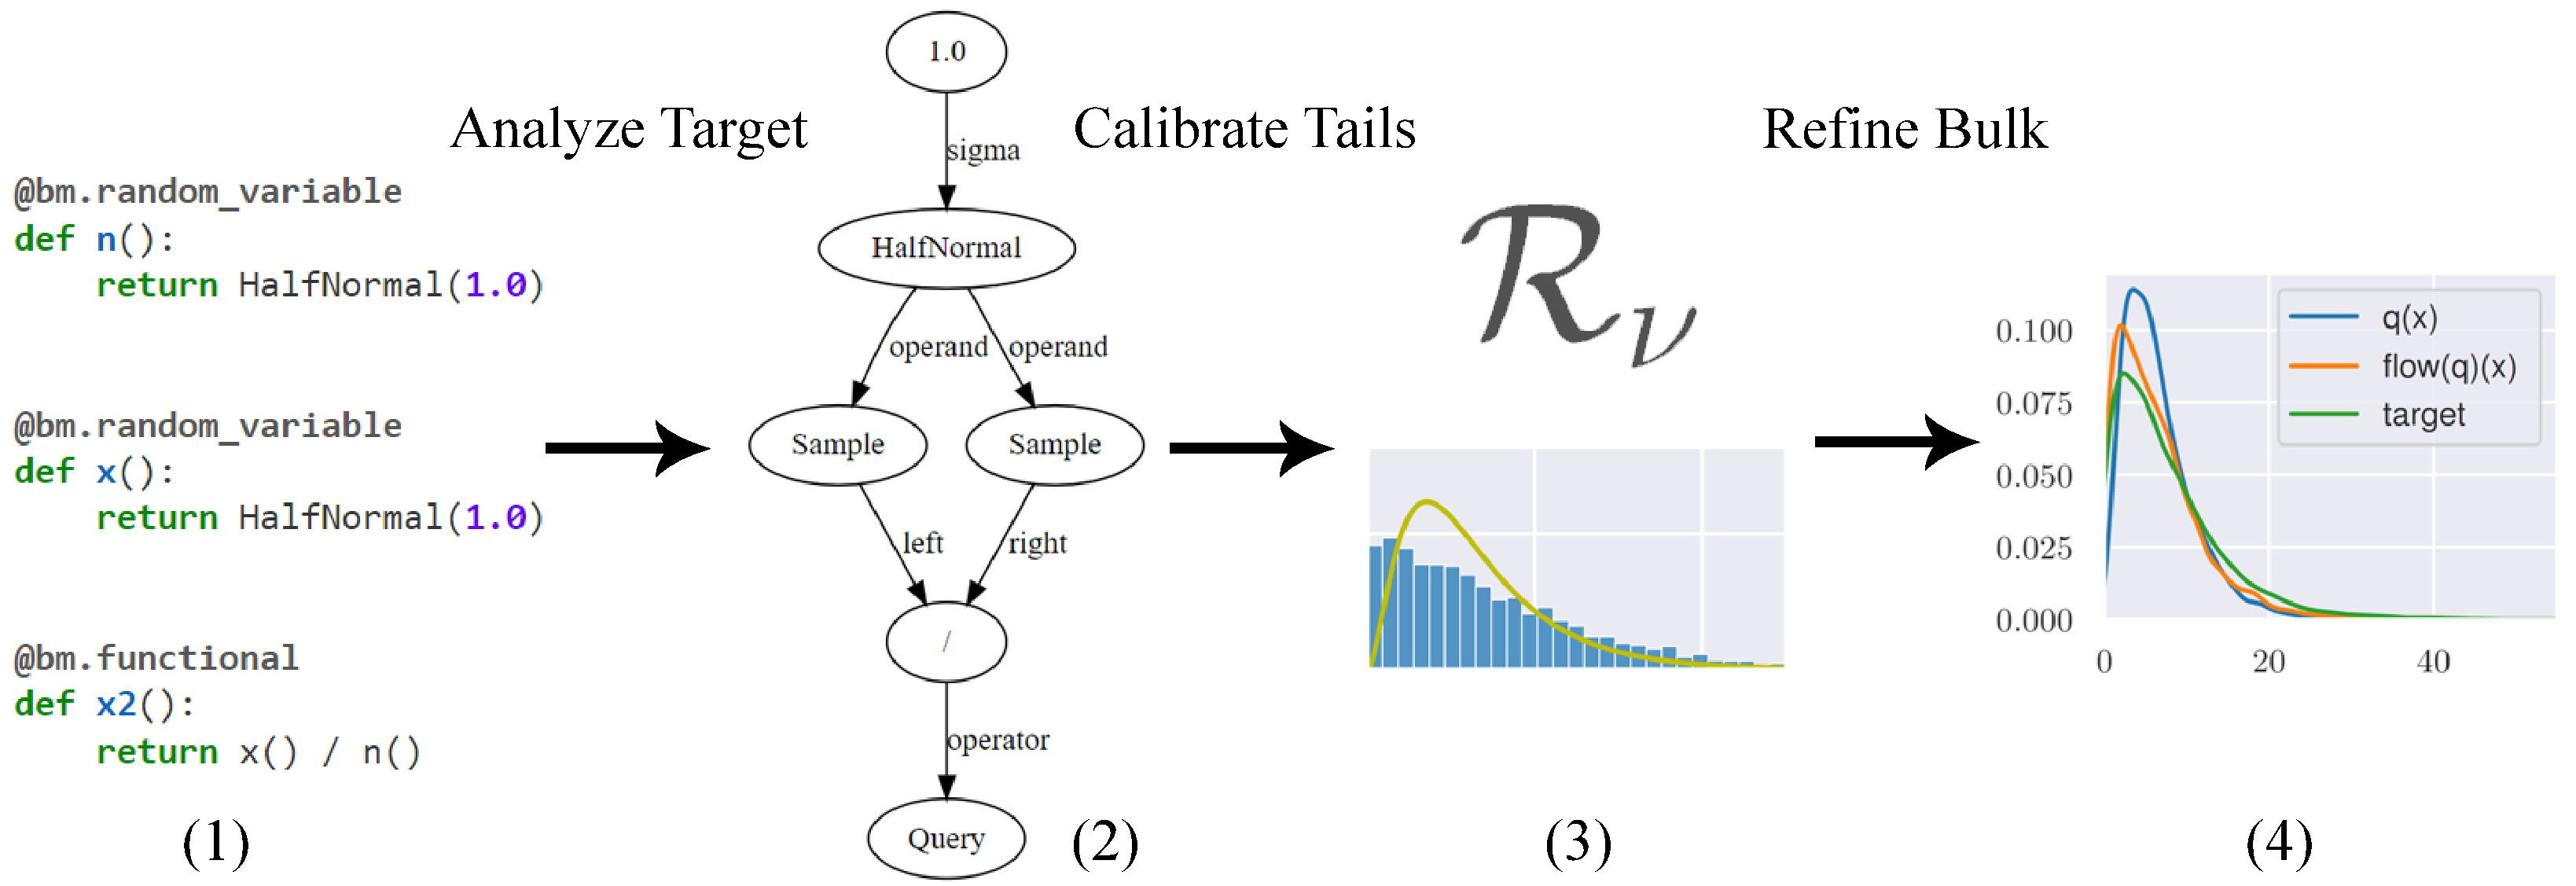
\includegraphics[width=\textwidth]{hta/figures/schematic.pdf}
  \caption{Our overall approach for density approximations with calibrated tails.
    A generative model expressed in a PPL (1) and analyzed using the GGA (2) to
    compute the tail parameters of the target. A representative distribution
    with calibrated tails is chosen for the initial approximation (3) and a learnable
    Lipschitz pushforward (see \Cref{lem:lipschitz}) is optimized (4) to correct the
    bulk approximation.}
\end{figure}



% \begin{wrapfigure}[18]{r}{0.35\textwidth}
% 	\centering
% 	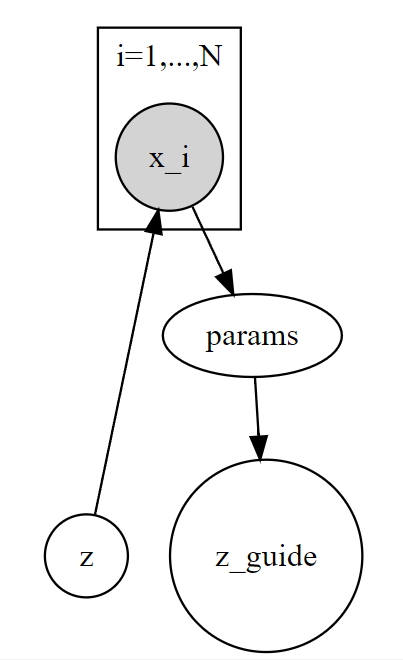
\includegraphics[width=.3\textwidth]{figures/pgm_vi.png}
% 	\caption{Graphical model and PPL API for VI with IID data $x_i$.}
% 	% 	Digraph fig1 {
% 	% rankdir = BT; //order things from left to right

% 	% { rank="same"; z; z_guide; }

% 	% //define alpha and beta as existing
% 	% z [shape=circle];
% 	% z_guide [shape=circle];

% 	% z->x_i; //quite literally z points at w

% 	% subgraph cluster_N
% 	% {
% 	%     label = "i=1,...,N"
% 	%     x_i [shape=circle, style=filled]
% 	% }
% 	% x_i -> params;
% 	% params -> z_guide

% 	% }
% \end{wrapfigure}

\textbf{Contributions}

\begin{itemize}[leftmargin=*]
  \item The GGA is introduced, generalizing prior work on classifying tail asymptotics
        while including both sub-Gaussian / sub-exponentials \citep{ledoux2001concentration} as well as power-law / Pareto-based tail indices \citep{clauset2009power}. Composing operations outlined in \cref{tab:gga_operations}, one can compute the
        GGA tail class for downstream random variables of interest.
  \item The GGA is implemented in the static analysis phase of a PPL compiler.
        This unlocks the ability to leverage GGA metadata in order to
        better tailor the emitted inference algorithm.
  \item Finally, we propose and evaluate a density estimator which combines GGA tails with normalizing flows
        in order to simultaneously achieve good bulk approximation as well as correct tails.
\end{itemize}

\section{Related Work}

\textbf{Heavy tails and probabilistic machine learning}

For studying heavy tails, methods based on subexponential distributions
\citep{goldie1998subexponential} and generalized Pareto distributions (GPD) or
equivalently regularly varying distributions \citep{tajvidi2003confidence}
have received attention historically. \citet{mikosch} presents closure theorems for regularly varying which are special cases of \Cref{prop:gga_add} and \Cref{lem:lipschitz}.
Heavy tails can impact probabilistic machine learning methods in a number of ways.
The observation that density ratios $\frac{p(x)}{q(x)}$ tend to be heavy tailed
has resulted in new methods for smoothing importance sampling \citep{vehtari2015pareto},
adaptively modifying divergences \citep{wang2018variational}, and
diagnosing variational inference through the Pareto $\hat{k}$ diagnostic \citep{yao2018yes}.
These works are complementary to our paper and our reported results include $\hat{k}$
diagnostics for VI and $\hat\alpha$ tail index estimates based on GPD.

Our work considers heavy-tailed targets $p(x)$ which is the same setting as
\citet{jaini2020tails,ftvi}. Whereas those respective works
lump the tail parameter in as another variational parameter and may be more generally applicable, the GGA may be applied before samples are drawn and leads to perfectly calibrated tails when applicable.

\textbf{Probabilistic programming}

PPLs can be characterized by the primary use case optimized for, whether that's
Gibbs sampling over Bayes nets \citep{spiegelhalter1996bugs,de2017programming},
stochastic control flow \citep{goodman2012church,wingate2011lightweight},
deep stochastic variational inference \citep{tran2018simple,bingham2019pyro}, or
Hamiltonian Monte-Carlo \citep{carpenter2017stan,xu2020advancedhmc}. Our implementation target
\texttt{beanmachine} \citep{tehrani2020bean} is a declarative PPL selected
due to availability of a PPL compiler and support for static analysis plugins.
Similar to \citet{bingham2019pyro,siddharth2017learning}, it uses PyTorch \citep{paszke2019pytorch} for GPU tensors and automatic differentiation.
Synthesizing an approximating distribution during PPL compilation (\Cref{sec:impl}) is
also performed in the Stan language by \citet{kucukelbir2017automatic} and normalizing
flow extensions in \citet{webb2019aml}. We compare directly against these related density approximators in \Cref{sec:hta:experiments}.

\textbf{Static analysis}

There is a long history of formal methods and probabilistic programming
\cite{kozen1979semantics,jones1989probabilistic}. While much of the research
\cite{claret2013bayesian}
is concerned with defining formal semantics
and establishing invariants \cite{wang2018pmaf}
See \cite{bernstein2019static} for a recent review.
Static analysis utilizes the abstract syntax tree (AST)
representation of a program in order to compute invariants
(e.g. the return type of a function, the number of classes implementing a trait)
without executing the underlying program.
As dynamic analysis in PPLs is less reliable due to non-determinism, static analysis
methods for PPLs become increasingly important.

Within PPLs, static analysis has traditionally been applied in the context of formalizing
semantics \citep{kozen1979semantics} and has been used to verify probabilistic
programs by ensuring termination, bounding random values values
\citep{sankaranarayanan2013static}. \cite{lee2019towards} proposes a static analyzer for the
Pyro PPL \citep{bingham2019pyro} to verify
distribution supports and avoid $-\texttt{Inf}$ log probabilities.


More relevant to our work are applications of static analysis to improve inference. \citet{nori2014r2} statically analyzes a probabilistic program and computes pre-images of observations in order to better adapt MCMC proposal distributions.
While we also perform static analysis over
abstract syntax tree (AST) representations of a probabilistic program,
applying GGA yields an upper bound on the tails of all random variables
so that calibrated tails can be imposed on distribution estimates.

\section{The Generalized Gamma Algebra}\label{sec:gga}

Here we formulate an algebra of random variables that is closed under most standard elementary operations (addition, multiplication, powers) which forms the foundation for our static analysis.

\begin{definition}\label{def:gg_tail}
  A random variable $X$ is said to have a \emph{generalized Gamma tail} if the Lebesgue density of $|X|$ satisfies
  \begin{equation}
    \label{eq:GenGammaTails}
    p_{|X|}(x) \sim c x^\nu e^{-\sigma x^\rho}, \qquad \text{as } x \to \infty,
  \end{equation}
  for some $c > 0$, $\nu \in \mathbb{R}$, $\sigma > 0$ and $\rho \in \mathbb{R}$. Denote the set of all such random variables by $\mathcal{G}$.
\end{definition}
Consider the following equivalence relation on $\mathcal{G}$: $X \equiv Y$ if and only if $0 < p_{|X|}(x) / p_{|Y|}(x) < +\infty$ for all sufficiently large $x$. The resulting equivalence classes can be represented by their corresponding parameters $\nu, \sigma, \rho$, and hence, we denote the class of random variables $X$ satisfying \cref{eq:GenGammaTails} by $(\nu,\sigma,\rho)$. In the special case where $\rho = 0$, for a fixed $\nu < -1$, each class $(\nu,\sigma,0)$ for $\sigma > 0$ is equivalent, and is denoted by $\mathcal{R}_{|\nu|}$, representing \emph{regularly varying} tails. Our algebra operates on these equivalence classes of $\mathcal{G}$, characterizing the change in tail behaviour under various operations.

\begin{table}[t]
  \centering
  \bgroup
  {\small
    \begin{tabular}{|M{0.15\linewidth} | p{0.75\linewidth}|}
      \hline
      \centering \multirow{2}{*}{\textbf{Ordering}}        &
      $\max\{(\nu_1,\sigma_1,\rho_1),(\nu_2,\sigma_2,\rho_2)\}$                                                                                                                                                                                                                    \\ & $\qquad \equiv \begin{cases}
          (\nu_1,\sigma_1,\rho_1) & \text{ if } \limsup_{x\to\infty} \frac{x^\nu_1 e^{-\sigma_1 x^{\rho_1}}}{x^\nu_2 e^{-\sigma_2 x^{\rho_2}}} < +\infty \\
          (\nu_2,\sigma_2,\rho_2) & \text{ otherwise.}
        \end{cases}$ \\ \hline
      \centering \multirow{2}{*}{\textbf{Addition}}        & $(\nu_{1},\sigma_{1},\rho_{1})\oplus(\nu_{2},\sigma_{2},\rho_{2})$                                                                                                                                                    \\
                                                           & $\equiv \begin{cases}
                                                                         \max\{(\nu_{1},\sigma_{1},\rho_{1}),(\nu_{2},\sigma_{2},\rho_{2})\}                                              & \text{ if }\rho_{1}\neq\rho_{2}\text{ or }\rho_{1},\rho_{2}<1 \\
                                                                         \left(\nu_{1}+\nu_{2}+1,\min\{\sigma_{1},\sigma_{2}\},1\right)                                                   & \text{ if }\rho_{1}=\rho_{2}=1                                \\
                                                                         (\nu_{1}+\nu_{2}+\frac{2-\rho}{2},(\sigma_{1}^{-\frac{1}{\rho-1}}+\sigma_{2}^{-\frac{1}{\rho-1}})^{1-\rho},\rho) & \text{ if }\rho=\rho_{1}=\rho_{2}>1.
                                                                       \end{cases}$
      \\ \hline
      \centering \textbf{Powers}                           & $(\nu,\sigma,\rho)^\beta \equiv (\frac{\nu+1}{\beta} - 1,\sigma,\frac{\rho}{\beta})$ for $\beta > 0$                                                                                                                  \\\hline
      \centering \textbf{Reciprocal*}                      & $(\nu,\sigma,\rho)^{-1} \equiv \begin{cases} (-\nu-2,\sigma,-\rho) & \text{ if } (\nu + 1)/\rho > 0 \text{ and } \rho \neq 0 \\
              \mathcal{R}_2         & \text{ otherwise}
                                                                                              \end{cases}$                                                                                          \\ \hline
      \centering \textbf{Scalar \linebreak Multiplication} & $c(\nu,\sigma,\rho) \equiv (\nu,\sigma/|c|^\rho,\rho)$                                                                                                                                                                \\\hline
      \multirow{3}{*}{\centering \textbf{Multiplication}}  & $(\nu_{1},\sigma_{1},\rho_{1})\otimes(\nu_{2},\sigma_{2},\rho_{2})$                                                                                                                                                   \\
                                                           & $\qquad \equiv\begin{cases}
                                                                               \left(\frac{1}{\mu}\left(\frac{\nu_{1}}{|\rho_{1}|}+\frac{\nu_{2}}{|\rho_{2}|}+\frac{1}{2}\right),\sigma,-\frac{1}{\mu}\right) & \text{ if }\rho_{1},\rho_{2}<0      \\
                                                                               \left(\frac{1}{\mu}\left(\frac{\nu_{1}}{\rho_{1}}+\frac{\nu_{2}}{\rho_{2}}-\frac{1}{2}\right),\sigma,\frac{1}{\mu}\right)      & \text{ if }\rho_{1},\rho_{2}>0      \\
                                                                               \mathcal{R}_{|\nu_1|}                                                                                                          & \mbox{ if }\rho_{1}\leq0,\rho_{2}>0 \\
                                                                               \mathcal{R}_{\min\{|\nu_1|,|\nu_2|\}}                                                                                          & \mbox{ if }\rho_{1}=0,\rho_{2}=0
                                                                             \end{cases}$                                    \\
                                                           & where $\mu=\frac{1}{|\rho_{1}|}+\frac{1}{|\rho_{2}|}=\frac{|\rho_{1}|+|\rho_{2}|}{|\rho_{1}\rho_{2}|}$, $\sigma=\mu(\sigma_{1}|\rho_{1}|)^{\frac{1}{\mu|\rho_{1}|}}(\sigma_{2}|\rho_{2}|)^{\frac{1}{\mu|\rho_{2}|}}$. \\ \hline
      \centering \textbf{Product of Densities}             & $(\nu_1,\sigma_1,\rho_1)\&(\nu_2,\sigma_2,\rho_2)
      \equiv \begin{cases}
                 (\nu_{1}+\nu_{2},\sigma_{1},\rho_{1})        & \text{ if }\rho_{1}<\rho_{2}      \\
                 (\nu_{1}+\nu_{2},\sigma_{1}+\sigma_{2},\rho) & \text{ if }\rho=\rho_{1}=\rho_{2} \\
                 (\nu_{1}+\nu_{2},\sigma_{2},\rho_{2})        & \text{ otherwise.}
               \end{cases}$                                                                                                                                                                                      \\ \hline
      \centering \textbf{Functions ($L$-Lipschitz)}        &
      $f(X_1,\dots,X_n) \equiv L \max\{X_1,\dots,X_n\}$                                                                                                                                                                                                                            \\ \hline
    \end{tabular}
  }
  \vspace{.25cm}
  \caption{\label{tab:gga_operations}Operations on random variables (e.g.$X_1 + X_2$) are
    viewed as actions on density functions
    (e.g. convolution $(\nu_1, \sigma_1, \rho_1)\oplus (\nu_2, \sigma_2, \rho_2)$) and the tail parameters of the result are analyzed and reported.}
  \egroup
\end{table}

The form of \cref{eq:GenGammaTails} and the name of the algebra is derived from the generalized Gamma distribution.
\begin{definition}
  Let $\nu \in \mathbb{R}$, $\sigma > 0$, and $\rho \in \mathbb{R} \backslash \{0\}$ be such that $(\nu+1)/ \rho > 0$.
  A non-negative random variable $X$ is \emph{generalized Gamma distributed} with parameters $\nu,\sigma,\rho$ if it has Lebesgue density
  \begin{equation}
    \label{eq:GenGammaDensity}
    p_{\nu,\sigma,\rho}(x) = c_{\nu,\sigma,\rho} x^\nu e^{-\sigma x^\rho},\qquad x > 0,
  \end{equation}
  where $c_{\nu,\sigma,\rho} = \rho \sigma^{(\nu+1)/\rho} / \Gamma((\nu+1)/\rho)$ is the normalizing constant. %The generalized Gamma density incorporates many other well-known densities, including that of the Gamma distribution ($\rho = 1$), and the Frechet/Weibull distribution ($\nu = \rho - 1$). 
\end{definition}
The importance of the generalized Gamma form arises due to a combination of two factors:
\begin{enumerate}[label={(\roman*)},leftmargin=*]
  \item The majority of interesting continuous univariate distributions with infinite support satisfy \cref{eq:GenGammaTails}, including
        Gaussians ($\nu=0$, $\rho=2$),
        gamma/exponential/chi-squared ($\nu > -1$, $\rho=1$), Weibull/Frechet ($\rho = \nu + 1$), and
        Student $T$/Cauchy/Pareto ($\mathcal{R}_\nu$).
        However, some notable exceptions include the log-normal distributions.
  \item The set $\mathcal{G}$ is known to be closed under additive convolution, positive powers, and Lipschitz functions --- we will show it is closed under multiplicative convolution as well. This covers the majority of elementary operations on independent random variables, with reciprocals, exponentials and logarithms the only exceptions. However, we will introduce a few ``tricks'' to handle these cases as well.
\end{enumerate}
The full list of operations in GGA is compiled in \cref{tab:gga_operations}. All operations in the GGA can be proven to exhibit identical behaviour with their corresponding operations on random variables, with the sole exception of reciprocals (marked by asterisk), where additional assumptions are required.

%To incorporate tails which lie outside of $\mathcal{G}$, we let $\mathcal{R}_1$ incorporate \emph{super-heavy tails}, which denote random variables with tails heavier than any random variable in $\mathcal{G}$. All operations remain consistent with this notation. Likewise, we let $\mathcal{L}$ denote \emph{super-light tails}, which are treated in our algebra as a class where $\rho = +\infty$ (effectively constants).

% \paragraph{Exponential and Logarithm.} Tails of the generalized Gamma form are not closed under exponentiation or logarithms. Indeed, if both $X$ and $\exp X$ have generalized Gamma tails, then $X$ is exponentially distributed (and $\exp X$ has power law tails). As a workaround, we can consider an upper bound on the tail by projecting onto the nearest possible exponentially distributed / power law tail. If $\rho > 1$, then a change of variables shows the density of $\exp X$ satisfies
% \[
% p_{\exp X}(x) \sim \frac{c}{x}(\log x)^{\nu}\exp\left(-\sigma(\log x)^{\rho}\right)\leq\frac{\tilde{c}}{x}\exp\left(-\sigma(\log x)\right)=cx^{-\sigma-1},\,\mbox{ as }x \to \infty.
% \]
% The inverse of this operation sends $\mathcal{R}_{\sigma+1}$ to $(0,\sigma,1)$. With this in mind, we define the exponential and logarithmic operations according to the following: $\exp (\nu, \sigma, \rho) \equiv \mathcal{R}_{\sigma+1}$ if $\rho \geq 1$, otherwise $\mathcal{R}_1$; $\log (\nu, \sigma, \rho) \equiv (0, |\nu|-1, 1)$ if $\nu < -1$ and $\rho \leq 0$, otherwise $\mathcal{L}$.

\subsection{Illustrative examples}\label{sec:addtl_eg}

To further illustrate the GGA through example, in this section we work
out explicit GGA computations using distributions
from \cref{tab:dist_list} and operations in \cref{tab:gga_operations}
and recover some common probability identities.

\begin{example}[Chi-squared random variables]
  Let $X_1,\dots,X_k$ be $k$ independent standard normal random variables. The variable $Z = \sum_{i=1}^k X_i^2$ is \emph{chi-squared distributed} with $k$ degrees of freedom. Using the generalized Gamma algebra, we can accurately determine the tail behaviour of this random variable directly from its construction. Recall that each $X_i \equiv (0,1/2,2)$, and by the power operation, $X_i^2 \equiv (-1/2,1/2,1)$. Applying the addition operation $k$ times reveals that $Z \equiv (k/2-1,1/2,1)$ and implies that the density of $Z$ is asymptotically $c x^{k/2-1} e^{-x / 2}$ as $x \to \infty$. In fact, the density of $Z$ is exactly $p_Z(x) = c_k x^{k/2-1} e^{-x/2}$ where $c_k = 2^{-k/2} / \Gamma(k/2)$.
\end{example}

\begin{example}[Products of random variables]
  To demonstrate the efficacy of the multiplication operation in our algebra, we consider the product of two exponential, Gaussian, and reciprocal Gaussian random variables. In \cref{sec:proofs}, we manually prove the following.
  \begin{lemma}
    \label{lem:Products}
    Let $X_1,X_2 \sim \mbox{Exp}(\lambda)$ and $Z_1,Z_2 \sim \mathcal{N}(0,1)$ be independent. The densities of $X_1 X_2$, $Z_1 Z_2$ and $Z = 1/Z_1 \cdot 1/Z_2$ satisfy as $x \to \infty$,
    \[
      p_{X_1 X_2}(x) \sim \frac{\lambda^{3/2}\sqrt{\pi}}{x^{1/4}} e^{-2\lambda \sqrt{x}},\quad p_{Z_1 Z_2}(x) \sim \frac{1}{\sqrt{2\pi x}} e^{-x},\quad
      p_{Z}(x) \sim \frac{1}{\sqrt{2\pi}|z|^{3/2}}e^{-1/|z|}.
    \]
  \end{lemma}
  With ease, our algebra correctly determines that $X_1 X_2 \equiv (-\frac14,2\lambda,\frac12)$, $Z_1 Z_2 \equiv (-\frac12, 1, 1)$ and $Z \equiv (-\frac32,1,-1)$.
  % Recall that the Bessel $K$-function of zeroth order, denoted $K_0$, is given by the Fourier transform $K_0(x) = \frac12 \int_{-\infty}^{\infty} e^{ixt} (1+t^2)^{-1/2} \dd t$. This function behaves as $x \to \infty$ as $K_{0}(x)\sim\sqrt{\frac{\pi}{2x}}e^{-x}$. Let $X_1,X_2 \sim \mathrm{Exp}(\lambda)$ be two independent exponentially distributed variables. The density of the product $Z = X_1 X_2$ is given by 
  % \[
  % p_Z(x) = 2\lambda^{2}K_{0}(2\lambda\sqrt{z})\sim\lambda^{3/2}\sqrt{\pi}z^{-1/4}e^{-2\lambda\sqrt{z}}.
  % \]
  % This tail behaviour can be obtained using our algebra as follows: 
  % The density of
  % \[
  % p_Z(x) = \frac1\pi K_0(|x|) \sim \frac{1}{\sqrt{2\pi x}} e^{-x},\qquad \mbox{as }x \to \infty.
  % \]
\end{example}


\begin{example}[Reciprocal distributions]
  Perhaps the most significant challenge with a tail algebra is correctly identifying the tail behaviour of reciprocal distributions. Here, we test the efficacy of our formulation with known reciprocal distributions.
  \begin{itemize}
    \item \emph{Reciprocal normal:} $X \sim \mathcal{N}(0,1) \equiv (0,1/2,2)$, and $X^{-1} \equiv (-2,1/2,-2)$.
    \item \emph{Inverse exponential:} $X \sim \text{Exp}(\lambda) \equiv (0,\lambda,1)$, and $X^{-1} \equiv (-2,\lambda,-1)$.
    \item \emph{Inverse $t$-distribution:} $X \equiv \mathcal{R}_\nu$, and $X^{-1} \equiv \mathcal{R}_2$.
    \item \emph{Inverse Cauchy:} $X \equiv \mathcal{R}_2$, it is known $X^{-1}$
          has the same distribution and our theory predicts $X^{-1} \equiv \mathcal{R}_2$.
  \end{itemize}
\end{example}

\begin{example}[Cauchy distribution]
  A simple special case of the Student $T$ distribution is the Cauchy distribution, which arises as the ratio of two standard normal random variables. For $X\sim\mathcal{N}(0,1)$, $X \equiv (0,1/2,2)$ and $X^{-1} \equiv (-2,1/2,-2)$. %The reciprocal of a standard normal random variable $X \equiv (0,1/2,2)$ satisfies $X^{-1} \equiv (-2,1/2,-2)$. 
  Hence, the multiplication operation correctly predicts that the ratio of two standard normal random variables is in $\mathcal{R}_2$.
\end{example}


\begin{example}[Student $T$ distribution]
  Let $X$ be a standard normal random variable, and $V$ a chi-squared random variable with $\nu$ degrees of freedom. The random variable $T = X / \sqrt{V / \nu}$ is \emph{$t$-distributed} with $\nu$ degrees of freedom. Since $V \equiv (\nu/2-1,1/2,1)$, multiplying by the constant $1/\nu$ reveals $V / \nu \equiv (\nu/2-1,1/(2\nu),1)$. Applying the square root operation, $\sqrt{V / \nu} \equiv (\nu-1,1/(2\nu),2)$. To compute the division operation, we first take the reciprocal to find $(V/\nu)^{-1/2} \equiv (-\nu-1,1/(2\nu),-2)$. Finally, since $\rho = -2 < 1$ for this random variable, the multiplication operation with $X \equiv (0,1/2,2)$ yields $T \equiv \mathcal{R}_{\nu+1}$, and so the density of $T$ is asymptotically $c x^{-\nu-1}$ as $x \to \infty$.
  Indeed, the density of $T$ satisfies $p_T(x) = c_\nu (1 + x^2 / \nu)^{-(\nu+1)/2}$ where $c_\nu = \Gamma(\frac{\nu+1}{2})/\Gamma(\frac{\nu}{2}) (\nu\pi)^{-1/2}$, which exhibits the predicted tail behaviour.
\end{example}


\begin{example}{Log-normal distribution}
  Although the log-normal distribution does not lie in $\mathcal{G}$, the existence of log-normal tails arising from the multiplicative central limit theorem is suggested by our algebra. Let $X_1,X_2,\dots$ be independent standard normal random variables and let $Z_k = X_1\cdots X_{2^k}$ for each $k=1,2,\dots$. By the multiplicative central limit theorem, letting $\tau = \exp(\mathbb{E}\log |X_i|) \approx 1.13$, $\left(\frac{X_{1}\cdots X_{n}}{\tau}\right)^{1/\sqrt{n}}$ converges in distribution as $n\to\infty$ to a log-normal random variable $Z$ with density
  \[
    p_Z(x) = \frac{1}{x\sqrt{2\pi}} \exp(-\tfrac12 (\log x)^2).
  \]
  Therefore, the same is true for $V_k = (Z_k / \tau)^{2^{-k/2}}$. Using our algebra, we will attempt to reproduce the tail of this density. Letting $\tilde{Z}_k = X_{2^k} \cdots X_{2^{k+1}}$, we see that $Z_{k+1} = Z_k \tilde{Z}_k$, and $Z_k,\tilde{Z}_k$ are iid. Let $Z_k \equiv (\nu_k, \sigma_k, \rho_k)$, by induction using the multiplication operation, we find that $\nu_{k+1} ~=~\frac{1}{\mu}\left(\frac{2\nu_{k}}{\rho_{k}}-\frac{1}{2}\right)=\nu_{k}-\frac{\rho_{k}}{4}$, $\sigma_{k+1}=\mu\left(\sigma_{k}\rho_{k}\right)^{\frac{2}{\mu\rho_{k}}}=\frac{2}{\rho_{k}}\left(\sigma_{k}\rho_{k}\right)=2\sigma_{k}$, and $\rho_{k+1}=\frac{1}{\mu}=\frac{\rho_{k}}{2}$.
  Since $\rho_0 = 2$, $\sigma_0 = 1/2$, and $\nu_0 = 0$, we find that $\rho_k = 2^{1-k}$ and $\sigma_k = 2^{k-1}$. Furthermore, $\nu_{k+1} = \nu_k - 2^{-k-1}$ and so $\nu_k = -1 + 2^{-k}$. Therefore $Z_k \equiv (-1+2^{-k},2^{k-1},2^{1-k})$, and
  \[
    V_k \equiv (-1+2^{-k/2},2^{k-1}\tau^{-2^{1-k}},2^{1-k/2}),
  \]
  and letting $\epsilon_k = 2^{-k/2}$, the tail behaviour of the density of $V_k$ satisfies
  \begin{align*}
    p_k(x) & \sim c_k x^{-1+\epsilon_{k}}\exp\left(-\frac{\epsilon_{k}^{-2}}{2\tau^{-2\epsilon_{k}^{2}}}x^{2\epsilon_k}\right) \\& \sim c_k x^{-1+\epsilon_{k}}\exp\left(-\frac{1}{2\tau^{-2\epsilon_{k}^{2}}}\left(\frac{x^{\epsilon_{k}}-1}{\epsilon_{k}}\right)^{2}\right) \approx c_k x^{-1}\exp\left(-\frac{1}{2}(\log x)^2\right),
  \end{align*}
  as $x \to \infty$, where the approximation improves as $k$ gets larger. The quality of this approximation is shown in \cref{fig:lognormal}.
\end{example}

\begin{figure}[h]
  \centering
  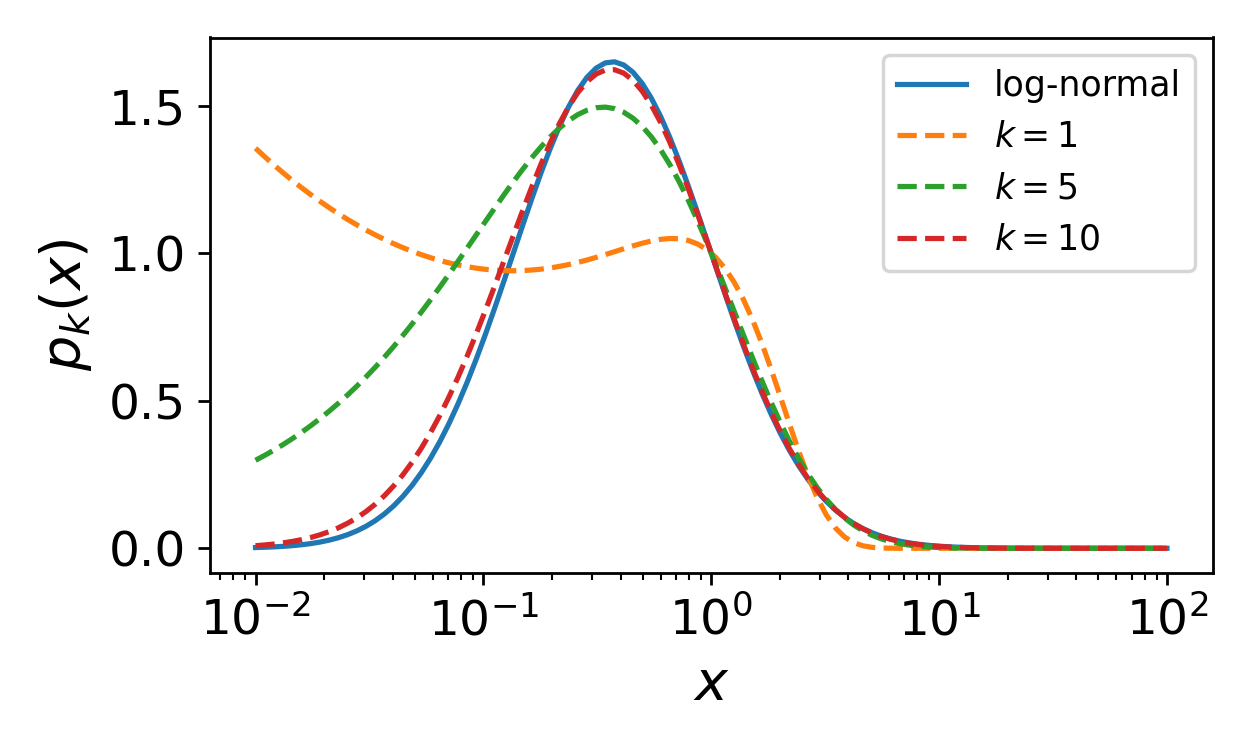
\includegraphics[width=0.4\textwidth]{figures/LogNormal_Bulk.png}
  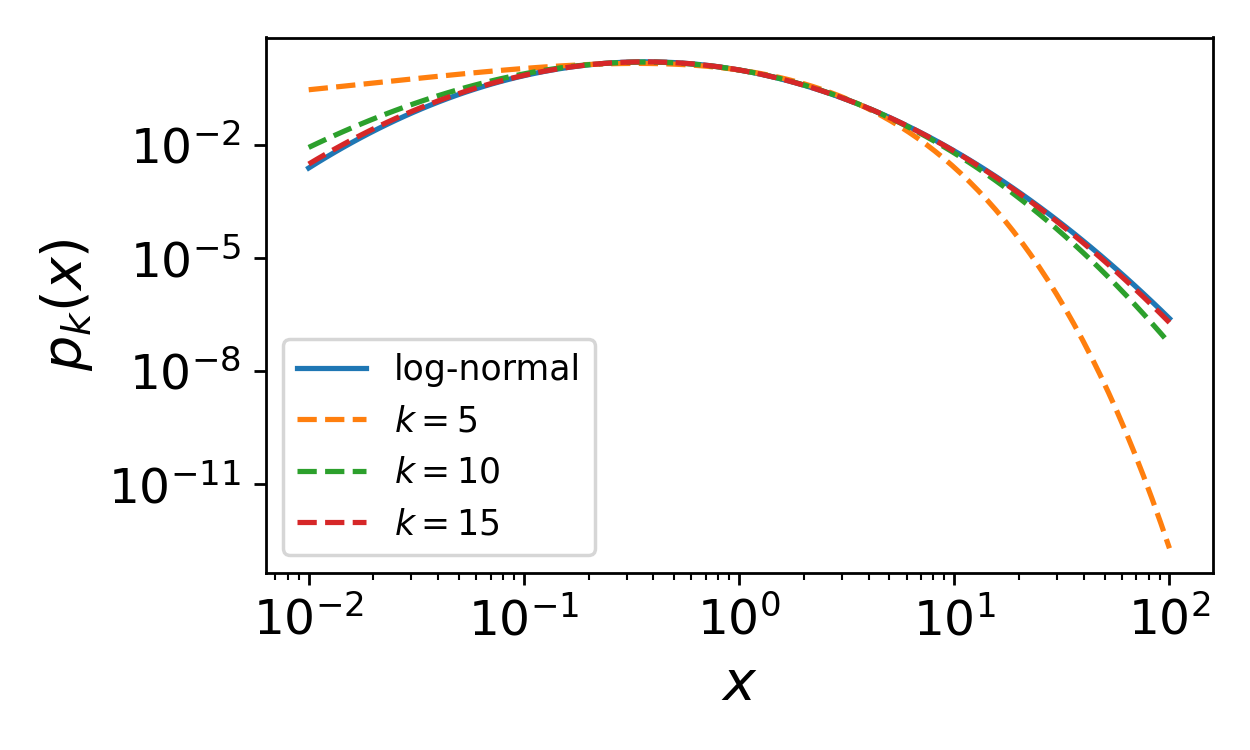
\includegraphics[width=0.4\textwidth]{figures/LogNormal_Tail.png}
  \caption{Estimation of the log-normal density by tail algebra applied to $V_k$.}
  \label{fig:lognormal}
\end{figure}

\subsection{Operations in the Generalized Gamma Algebra}

Whereas \cref{tab:gga_operations} provides a summary of our theory useful
for referencing, in this section we provide additional explanation and references
for how operations on random variables affect their GGA tails.

\paragraph{Ordering.} A total ordering is imposed on the equivalence classes of $\mathcal{G}$ according to the heaviness of tails. In particular, we say that $(\nu_1,\sigma_1,\rho_1) \leq (\nu_2,\sigma_2,\rho_2)$ if $(x^{\nu_1} e^{-\sigma_1 x^{\rho_1}}) / (x^{\nu_2} e^{-\sigma_2 x^{\rho_2}})$ is bounded as $x \to \infty$. As usual, we say $(\nu_1,\sigma_1,\rho_1) < (\nu_2,\sigma_2,\rho_2)$ if $(\nu_1,\sigma_1,\rho_1) \leq (\nu_2,\sigma_2,\rho_2)$ but $(\nu_1,\sigma_1,\rho_1) \not\equiv (\nu_2,\sigma_2,\rho_2)$.

%\paragraph{Multiplication by a Constant.} 

\paragraph{Addition.} Tails of this form are  closed under addition. Combining subexponentiality for $\rho < 1$
%Any random variable $X$ in $(\nu,\sigma,\rho)$ for $\rho < 1$ is subexponential 
\cite[Chapter X.1]{asmussen2010ruin},
%that is, any sum of iid copies of $X$ asymptotically saturates the union bound: $\mathbb{P}\left(\sum_{i=1}^{n}X_{i}>x\right)\sim\sum_{i=1}^{n}\mathbb{P}(X_{i}>x)$ as $x \to \infty$. Combining this
with \cite[Thm 3.1 \& eqn. (8.3)]{asmussen2017tail},
\begin{proposition}
  \label{prop:gga_add}
  Denoting the addition of random variables (additive convolution of densities) by $\oplus$,
  \begin{multline}
    (\nu_{1},\sigma_{1},\rho_{1})\oplus(\nu_{2},\sigma_{2},\rho_{2})
    \\\equiv \begin{cases}
      \max\{(\nu_{1},\sigma_{1},\rho_{1}),(\nu_{2},\sigma_{2},\rho_{2})\}                                              & \text{ if }\rho_{1}\neq\rho_{2}\text{ or }\rho_{1},\rho_{2}<1 \\
      \left(\nu_{1}+\nu_{2}+1,\min\{\sigma_{1},\sigma_{2}\},1\right)                                                   & \text{ if }\rho_{1}=\rho_{2}=1                                \\
      (\nu_{1}+\nu_{2}+1-\frac{\rho}{2},(\sigma_{1}^{-\frac{1}{\rho-1}}+\sigma_{2}^{-\frac{1}{\rho-1}})^{1-\rho},\rho) & \text{ if }\rho=\rho_{1}=\rho_{2}>1.
    \end{cases}
  \end{multline}
\end{proposition}

\paragraph{Powers.} For all exponents $\beta > 0$, by invoking a change of variables $x \mapsto x^\beta$, it is easy to show that
%\begin{equation}
%\label{eq:PowerEqn}
$(\nu, \sigma, \rho)^\beta \equiv  \left(\frac{\nu+1}{\beta}-1, \sigma, \frac{\rho}\beta\right).$
%\end{equation}
%\paragraph{Reciprocals.}
We \emph{define} negative powers and reciprocals equivalently to positive powers in the case $\beta < 0$. This equivalence cannot be proven to hold in general since we cannot determine tail asymptotics of the reciprocal without knowledge of its behaviour around zero. Therefore, we implicitly assume that the behaviour around zero mimics the tail behaviour, that is, \cref{eq:GenGammaTails} holds as $x \to 0^+$. However, this can only hold provided $(\nu + 1)/\rho > 0$ and $\rho \neq 0$. In all other cases, including $\mathcal{R}_\nu$, we assume that the density of $X$ approaches a nonzero value near zero, and define the reciprocal to be $\mathcal{R}_{2}$. %By assuming $p_X(x) \to \tilde{c} x^\nu e^{-\sigma x^\rho}$ as $x \to 0^+$, then \cref{eq:PowerEqn} also holds for $\beta < 0$.

\paragraph{Multiplication.}
For any $c \in \mathbb{R} \backslash \{0\}$, it can be readily seen from a change of variables $x \mapsto c x$ that $c (\nu, \sigma, \rho) = (\nu, \sigma / |c|^\rho, \rho)$. The class $\mathcal{G}$ is also closed under multiplication (assuming independence of random variables), as we show in the following result --- the proof is delayed to Appendix C.
\begin{proposition}
  \label{prop:Mult}
  Denoting the multiplication of independent random variables (multiplicative convolution) by $\otimes$,
  \[
    (\nu_{1},\sigma_{1},\rho_{1})\otimes(\nu_{2},\sigma_{2},\rho_{2})
    \equiv\begin{cases}
      \left(\frac{1}{\mu}\left(\frac{\nu_{1}}{|\rho_{1}|}+\frac{\nu_{2}}{|\rho_{2}|}+\frac{1}{2}\right),\sigma,-\frac{1}{\mu}\right) & \text{ if }\rho_{1},\rho_{2}<0      \\
      \left(\frac{1}{\mu}\left(\frac{\nu_{1}}{\rho_{1}}+\frac{\nu_{2}}{\rho_{2}}-\frac{1}{2}\right),\sigma,\frac{1}{\mu}\right)      & \text{ if }\rho_{1},\rho_{2}>0      \\
      \mathcal{R}_{|\nu_1|}                                                                                                          & \mbox{ if }\rho_{1}\leq0,\rho_{2}>0 \\
      \mathcal{R}_{\min\{|\nu_1|,|\nu_2|\}}                                                                                          & \mbox{ if }\rho_{1}=0,\rho_{2}=0
    \end{cases}
  \]
  where $\mu=\frac{1}{|\rho_{1}|}+\frac{1}{|\rho_{2}|}=\frac{|\rho_{1}|+|\rho_{2}|}{|\rho_{1}\rho_{2}|}$ and $\sigma=\mu(\sigma_{1}|\rho_{1}|)^{\frac{1}{\mu|\rho_{1}|}}(\sigma_{2}|\rho_{2}|)^{\frac{1}{\mu|\rho_{2}|}}$.
\end{proposition}
% \begin{proof}
% Appendix C.
% \end{proof}

%\feynman{I added this back; we need it for the StudentT example but this result currently doesn't give what we need}
%The next binary operation of interest is \emph{multiplication}. Using Cauchy's inequality, we can adopt the naive
%\[
%X \cdot Y \equiv \max\{X^2, Y^2\}.
%\]
%In the case where $X,Y \in \mathcal{E}$, this turns out to be reasonable. However, for any other use case, Breiman's lemma suggests that $X \cdot Y \equiv \max\{X, Y\}$. \todo{Perform Tauberian analysis to determine sharpness of these operations}.


\paragraph{Product of Densities.}

We can also consider a product of densities operation acting on two random variables $X,Y$, denoted $X \& Y$, by
$p_{X \& Y}(x) = c p_X(x) p_Y(x)$,
where $c > 0$ is an appropriate normalizing constant and $p_X,p_Y,p_{X\& Y}$ are the densities of $X$, $Y$, and $X \& Y$, respectively. In terms of the equivalence classes:
\[
  (\nu_1,\sigma_1,\rho_1)\&(\nu_2,\sigma_2,\rho_2)
  \equiv \begin{cases}
    (\nu_{1}+\nu_{2},\sigma_{1},\rho_{1})        & \text{ if }\rho_{1}<\rho_{2}      \\
    (\nu_{1}+\nu_{2},\sigma_{1}+\sigma_{2},\rho) & \text{ if }\rho=\rho_{1}=\rho_{2} \\
    (\nu_{1}+\nu_{2},\sigma_{2},\rho_{2})        & \text{ otherwise.}
  \end{cases}
\]
Note that this particular operation does not require either $p_X$ or $p_Y$ to be normalized --- only the tail behaviour is needed. We may also use this to work out the tail behaviour of a posterior density, provided the tail behaviour of the likelihood in the parameters is known.

\paragraph{Lipschitz Functions.}

There are many multivariate functions that cannot be readily represented in terms of the operations covered thus far. For these, it is important to specify the tail behaviour of pushforward measures under Lipschitz-continuous functions. Fortunately, this is covered by \cref{lem:lipschitz} below, presented in \cite[Proposition 1.3]{ledoux2001concentration}.
H\"{o}lder-continuous functions can also be represented as a composition of a power operation and a Lipschitz-continuous function.
\begin{lemma}\label{lem:lipschitz}
  For any Lipschitz continuous function $f:\mathbb{R}^d \to \mathbb{R}$ satisfying $\|f(x)-f(y)\|\leq L\|x -y\|$ for $x,y \in \mathbb{R}^d$, there is $f(X_1,\dots,X_d) \equiv L \max\{X_1,\dots,X_d\}.$
\end{lemma}

\paragraph{Power Law Approximation.} Note that as $x \to \infty$, $p_{|X|}(x) \sim c x^\nu e^{-\sigma x^\rho} = \tilde{c}x^\nu e^{-\sigma\rho\frac{x^\rho - 1}{\rho}} \approx \tilde{c} x^\nu e^{-\sigma\rho \log x}$
\[
  p_{|X|}(x) \sim c x^\nu e^{-\sigma x^\rho} = \tilde{c} x^\nu e^{-\sigma(x^\rho - 0)} = \tilde{c} x^\nu e^{-\sigma\rho\frac{x^\rho - 1}{\rho}} \approx \tilde{c} x^\nu e^{-\sigma\rho \log x} = \tilde{c} x^{\nu-\sigma \rho},
\]
where we have used the approximation $\log x = \rho^{-2}(x^\rho - 1) + \mathcal{O}(\rho^2)$. Consequently, we can represent tails of this form by the Student $t$ distribution with $|\nu-\sigma\rho|-1$ degrees of freedom. In practice, we find this approximation tends to \emph{overestimate} the heaviness of the tail. Alternatively, the generalized Gamma density (\ref{eq:GenGammaDensity}) satisfies $\mathbb{E}X^r = \sigma^{-r/\rho} \Gamma(\frac{\nu+1+r}{\rho})/\Gamma(\frac{\nu+1}{\rho})$ for $r > 0$. Let $\alpha > 0$ be such that $\mathbb{E}X^\alpha = 2$. By Markov's inequality, the tail of $X$ satisfies $\mathbb{P}(X>x)\leq 2 x^{-\alpha}$. Therefore, we can represent tails of this form by the Student $t$ distribution with $\alpha+1$ degrees of freedom (generate $X \sim t_{\alpha}$). In practice, we find this approximation to be more accurate, and is hence used in Section 4.1.

\subsection{List of univariate distributions}

Here we provide an enumeration of common parametric distributions and their
corresponding GGA parameterizations.

  {\small
    \bgroup
    \def\arraystretch{2}
    \begin{longtable}{|c|c|c|c|}
      \caption{List of univariate distributions}\label{tab:dist_list}                                                                                                                                                                                                                                                                         \\
      \hline
      Name                                                                  & Support                                                 & Density $p(x)$                                                                                                                  & Class\tabularnewline
      \hline
      \hline
      Benktander Type II                                                    & $(0,\infty)$                                            & $e^{\frac{a}{b}(1-x^{b})}x^{b-2}(ax^{b}-b+1)$                                                                                   & $(2b-2,\frac{a}{b},b)$\tabularnewline
      \hline
      Beta prime distribution                                               & $(0,\infty)$                                            & $\frac{\Gamma(\alpha+\beta)}{\Gamma(\alpha)\Gamma(\beta)}x^{\alpha-1}(1+x)^{-\alpha-\beta}$                                     & $\mathcal{R}_{\beta+1}$\tabularnewline
      \hline
      Burr distribution                                                     & $(0,\infty)$                                            & $ckx^{c-1} (1+x^{c})^{-k-1}$                                                                                                    & $\mathcal{R}_{ck+1}$\tabularnewline
      \hline
      Cauchy distribution                                                   & $(-\infty,\infty)$                                      & $(\pi\gamma)^{-1}\left[1+\left(\frac{x-x_{0}}{\gamma}\right)^{2}\right]^{-1}$                                                   & $\mathcal{R}_{2}$\tabularnewline
      \hline
      Chi distribution                                                      & $(0,\infty)$                                            & $\frac{1}{2^{k/2-1}\Gamma(k/2)}x^{k-1}e^{-x^{2}/2}$                                                                             & $(k-1,\frac{1}{2},2)$\tabularnewline
      \hline
      Chi-squared distribution                                              & $(0,\infty)$                                            & $\frac{1}{2^{k/2}\Gamma(k/2)}x^{\frac{k}{2}-1}e^{-x/2}$                                                                         & $(\frac{k}{2}-1,\frac{1}{2},1)$\tabularnewline
      \hline
      Dagum distribution                                                    & $(0,\infty)$                                            & $\frac{ap}{x}\left(\frac{x}{b}\right)^{ap}\left(\left(\frac{x}{b}\right)^{a}+1\right)^{-p-1}$                                   & $\mathcal{R}_{a+1}$\tabularnewline
      \hline
      Davis distribution                                                    & $(0,\infty)$                                            & $\propto(x-\mu)^{-1-n}/\left(e^{\frac{b}{x-\mu}}-1\right)$                                                                      & $(-1-n,b,-1)$\tabularnewline
      \hline
      Exponential distribution                                              & $(0,\infty)$                                            & $\lambda e^{-\lambda x}$                                                                                                        & $(0,\lambda,1)$\tabularnewline
      \hline
      $F$ distribution                                                      & $(0,\infty)$                                            & $\propto x^{d_{1}/2-1}(d_{1}x+d_{2})^{-(d_{1}+d_{2})/2}$                                                                        & $\mathcal{R}_{d_{2}/2+1}$\tabularnewline
      \hline
      Fisher $z$-distribution                                               & $(-\infty,\infty)$                                      & $\propto\frac{e^{d_{1}x}}{(d_{1}e^{2x}+d_{2})^{(d_{1}+d_{2})/2}}$                                                               & $(0,d_{2},1)$\tabularnewline
      \hline
      Frechet distribution                                                  & $(0,\infty)$                                            & $\frac{\alpha}{\lambda}\left(\frac{x-m}{\lambda}\right)^{-1-\alpha}e^{-\left(\frac{x-m}{\lambda}\right)^{-\alpha}}$             & $(-1-\alpha,\lambda^{\alpha},-\alpha)$\tabularnewline
      \hline
      Gamma distribution                                                    & $(0,\infty)$                                            & $\frac{\beta^{\alpha}}{\Gamma(\alpha)}x^{\alpha-1}e^{-\beta x}$                                                                 & $(\alpha-1,\beta,1)$\tabularnewline
      \hline
      Gamma/Gompertz distribution                                           & $(0,\infty)$                                            & $bse^{bx}\beta^{s}/(\beta-1+e^{bx})^{s+1}$                                                                                      & $(0,bs,1)$\tabularnewline
      \hline
      Gen. hyperbolic distribution                                          & $(-\infty,\infty)$                                      & $\propto e^{\beta(x-\mu)}\frac{K_{\lambda-1/2}(\alpha\sqrt{\delta^{2}+(x-\mu)^{2}})}{(\delta^{2}+(x-\mu)^{2})^{1/4-\lambda/2}}$ & $(\lambda-1,\alpha-\beta,1)$\tabularnewline
      \hline
      Gen. Normal distribution                                              & $(-\infty,\infty)$                                      & $\frac{\beta}{2\alpha\Gamma(1/\beta)}\exp\left(-\left(\frac{|x-\mu|}{\alpha}\right)^{\beta}\right)$                             & $(0,\alpha^{-\beta},\beta)$\tabularnewline
      \hline
      Geometric stable distribution                                         & $(-\infty,\infty)$                                      & no closed form                                                                                                                  & $\mathcal{R}_{\alpha+1}$\tabularnewline
      \hline
      Gompertz distribution                                                 & $(0,\infty)$                                            & $\sigma \eta \exp(\eta + \sigma x - \eta e^{\sigma x})$                                                                         & $\mathcal{L}$\tabularnewline
      \hline
      Gumbel distribution                                                   & $(0,\infty)$                                            & $\beta^{-1} e^{-(\beta^{-1}(x-\mu)+e^{-\beta^{-1}(x-\mu)})}$                                                                    & $(0,\frac{1}{\beta},1)$\tabularnewline
      \hline
      Gumbel Type II distribution                                           & $(0,\infty)$                                            & $\alpha\beta x^{-\alpha-1}e^{-\beta x^{-\alpha}}$                                                                               & $(-\alpha-1,\beta,-\alpha)$\tabularnewline
      \hline
      Holtsmark distribution                                                & $(-\infty,\infty)$                                      & no closed form                                                                                                                  & $\mathcal{R}_{5/2}$\tabularnewline
      \hline
      Hyperbolic secant distribution                                        & $(-\infty,\infty)$                                      & $\frac{1}{2}\text{sech}\left(\frac{\pi x}{2}\right)$                                                                            & $(0,\frac{\pi}{2},1)$\tabularnewline
      \hline
      Inv. chi-squared distribution                                         & $(0,\infty)$                                            & $\frac{2^{-k/2}}{\Gamma(k/2)}x^{-k/2-1}e^{-1/(2x)}$                                                                             & $(-\frac{k}{2}-1,\frac{1}{2},-1)$\tabularnewline
      \hline
      Inv. gamma distribution                                               & $(0,\infty)$                                            & $\frac{\beta^{\alpha}}{\Gamma(\alpha)}x^{-\alpha-1}e^{-\beta/x}$                                                                & $(-\alpha-1,\beta,-1)$\tabularnewline
      \hline
      Levy distribution                                                     & $(0,\infty)$                                            & $\sqrt{\frac{c}{2\pi}}(x-\mu)^{-3/2}e^{-\frac{c}{2(x-\mu)}}$                                                                    & $(-\frac{3}{2},\frac{c}{2},-1)$\tabularnewline
      \hline
      Laplace distribution                                                  & $(-\infty,\infty)$                                      & $\frac{1}{2\lambda}\exp\left(-\frac{|x-\mu|}{\lambda}\right)$                                                                   & $(0,\frac{1}{\lambda},1)$\tabularnewline
      \hline
      Logistic distribution                                                 & $(-\infty,\infty)$                                      & $\frac{e^{-(x-\mu)/\lambda}}{\lambda(1+e^{-(x-\mu)/\lambda})^{2}}$                                                              & $(0,\frac{1}{\lambda},1)$\tabularnewline
      \hline
      Log-Cauchy distribution                                               &
      $(0,\infty)$                                                          & $\frac{\sigma}{x\pi}((\log x - \mu)^2 + \sigma^2)^{-1}$ & $\mathcal{R}_1$\tabularnewline
      \hline
      Log-Laplace distribution                                              & $(0,\infty)$                                            & $\frac{1}{2\lambda x}\exp\left(-\frac{\left|\log x-\mu\right|}{\lambda}\right)$                                                 & $\mathcal{R}_{1/\lambda+1}$\tabularnewline
      \hline
      Log-logistic distribution                                             & $(0,\infty)$                                            & $\frac{\beta}{\alpha}\left(\frac{x}{\alpha}\right)^{\beta-1}\left(1+\left(\frac{x}{\alpha}\right)^{\beta}\right)^{-2}$          & $\mathcal{R}_{\beta+1}$\tabularnewline
      \hline
      Log-$t$ distribution                                                  &
      $(0,\infty)$                                                          &
      $\propto x^{-1} (1 + \frac1{\nu}(\log x - \mu)^2)^{-\frac{\nu+1}{2}}$ & $\mathcal{R}_1$\tabularnewline
      \hline
      Lomax distribution                                                    & $(0,\infty)$                                            & $\frac{\alpha}{\lambda}\left(1+\frac{x}{\lambda}\right)^{-\alpha-1}$                                                            & $\mathcal{R}_{\alpha+1}$\tabularnewline
      \hline
      Maxwell-Boltzmann distribution                                        & $(0,\infty)$                                            & $\sqrt{\frac{2}{\pi}}\frac{x^{2}e^{-x^{2}/(2\sigma^{2})}}{\sigma^{3}}$                                                          & $(2,\frac{1}{2\sigma^{2}},2)$\tabularnewline
      \hline
      Normal distribution                                                   & $(-\infty,\infty)$                                      & $\frac{1}{\sigma\sqrt{2\pi}}e^{-\frac{1}{2}(\frac{x-\mu}{\sigma})^{2}}$                                                         & $(0,\frac{1}{2\sigma^{2}},2$)\tabularnewline
      \hline
      Pareto distribution                                                   & $(x_{0},\infty)$                                        & $\alpha x_{0}^{\alpha}x^{-\alpha-1}$                                                                                            & $\mathcal{R}_{\alpha+1}$\tabularnewline
      \hline
      Rayleigh distribution                                                 & $(0,\infty)$                                            & $\frac{x}{\sigma^{2}}e^{-x^{2}/(2\sigma^{2})}$                                                                                  & $(1,\frac{1}{2\sigma^{2}},2)$\tabularnewline
      \hline
      Rice distribution                                                     & $(0,\infty)$                                            & $\frac{x}{\sigma^{2}}\exp\left(-\frac{(x^{2}+\nu^{2})}{2\sigma^{2}}\right)I_{0}\left(\frac{x\nu}{\sigma^{2}}\right)$            & $(\frac{1}{2},\frac{1}{2\sigma^{2}},2)$\tabularnewline
      \hline
      Skew normal distribution                                              & $(-\infty,\infty)$                                      & no closed form                                                                                                                  & $(0,\frac{1}{2\sigma^{2}},2)$\tabularnewline
      \hline
      Slash distribution                                                    & $(-\infty,\infty)$                                      & $\frac{1-e^{-\frac{1}{2}x^{2}}}{\sqrt{2\pi}x^{2}}$                                                                              & $(-2,\frac{1}{2},2)$\tabularnewline
      \hline
      Stable distribution                                                   & $(-\infty,\infty)$                                      & no closed form                                                                                                                  & $\mathcal{R}_{\alpha+1}$\tabularnewline
      \hline
      Student's $t$-distribution                                            & $(-\infty,\infty)$                                      & $\frac{\Gamma(\frac{\nu+1}{2})}{\sqrt{\nu\pi}\Gamma(\frac{\nu}{2})}\left(1+\frac{x^{2}}{\nu}\right)^{-\frac{\nu+1}{2}}$         & $\mathcal{R}_{\nu+1}$\tabularnewline
      \hline
      Tracy-Widom distribution                                              & $(-\infty,\infty)$                                      & no closed form                                                                                                                  & $(-\frac{3\beta}{4}-1,\frac{2\beta}{3},\frac{3}{2})$\tabularnewline
      \hline
      Voigt distribution                                                    & $(-\infty,\infty)$                                      & no closed form                                                                                                                  & $\mathcal{R}_{2}$\tabularnewline
      \hline
      Weibull distribution                                                  & $(0,\infty)$                                            & $\frac{\rho}{\lambda}\left(\frac{x}{\lambda}\right)^{\rho-1}e^{-(x/\lambda)^{\rho}}$                                            & $(\rho-1,\lambda^{-\rho},\rho)$\tabularnewline
      \hline
    \end{longtable}
    \egroup
  }

The following densities are not supported by our algebra: Benini distribution; Benktander Type I distribution; Johnson's $S_U$-distribution; and the log-normal distribution. All of these densities exhibit log-normal tails.

\subsection{Proofs of new results}
\label{sec:proofs}

\begin{proof}[Proof of Lemma \ref{lem:Products}]
  The proof relies on the following integral definition \cite[pg. 183]{watson1995treatise} and asymptotic relation as $z \to \infty$ \cite[pg. 202]{watson1995treatise} of the modified Bessel function $K_\nu(z)$ for $z > 0$ and $\nu \geq 0$,
  \begin{equation}
    \label{eq:BesselInt}
    K_\nu(z) = \frac12 \left(\frac{z}{2}\right)^\nu \int_0^\infty u^{-\nu-1}\exp\left(-u - \frac{z^2}{4u}\right) \dd u \sim \sqrt{\frac{\pi}{2z}}e^{-z}.
  \end{equation}
  We also make use of the known density for the product of two independent continuous random variables: if $X$ and $Y$ have densities $p_X$ and $p_Y$ respectively, then $Z = XY$ has density
  \[
    p_Z(z) = \int_\mathbb{R} p_X(x) p_Y(z/x) |x|^{-1} \dd x.
  \]
  \paragraph{Exponentials.} Recalling that the density of $X \sim \mathrm{Exp}(\lambda)$ is $p_X(x) = \lambda e^{-\lambda x}$ for $x \geq 0$, for $Z = XY$ where $X \sim \mathrm{Exp}(\lambda_1)$ and $Y \sim \mathrm{Exp}(\lambda_2)$ are independent,
  \[
    p_Z(z) = \int_{0}^{\infty}x^{-1}\lambda_{1}e^{-\lambda_{1}x}\lambda_{2}e^{-\lambda_{2}z/x}\dd x = \lambda_{1}\lambda_{2}\int_{0}^{\infty}x^{-1}e^{-\lambda_{1}x-\lambda_{2}z/x}\dd x.
  \]
  Since $2K_{0}(2\sqrt{z})=\int_{0}^{\infty}u^{-1}\exp(-u-\frac{z}{u})\dd u$, let $u = \lambda_1 v$, so that $\dd u = \lambda_1 \dd v$,
  \[
    2K_{0}(2\sqrt{\lambda_{1}\lambda_{2}z})=\int_{0}^{\infty}u^{-1}\exp\left(-\lambda_{1}v-\lambda_{2}\frac{z}{v}\right)\dd v.
  \]
  Therefore, letting $\lambda = \sqrt{\lambda_1\lambda_2}$,
  \[
    p_Z(z) = 2\lambda^2 K_0(2\lambda\sqrt{z}) \sim \sqrt{\pi} \lambda^{3/2} z^{-1/4} e^{-2\lambda z^{1/2}}.
  \]
  \paragraph{Normals.} Recalling that the density of $X \sim \mathcal{N}(0,1)$ is $p_X(x) = (2\pi)^{-1/2} \exp(-\frac12 x^2)$, for $Z = XY$ where $X,Y \sim \mathcal{N}(0,1)$ are independent,
  \begin{align*}
    p_Z(z) & = \frac{1}{2\pi}\int_{\mathbb{R}}\left|x\right|^{-1}e^{-\frac{1}{2}x^{2}}e^{-\frac{1}{2}z^{2}/x^{2}}\dd x \\
           & =\frac{1}{\pi}\int_{0}^{\infty}x^{-1}e^{-\frac{1}{2}x^{2}-\frac{1}{2}z^{2}/x^{2}}\dd x                    \\
           & =\frac{1}{\pi}\int_{0}^{\infty}x^{-1}e^{-\frac{1}{2}x^{2}-\frac{1}{2}z^{2}/x^{2}}\dd x.
  \end{align*}
  Let $u=\frac{1}{2}x^{2}$ so that $\dd u=x \dd x$ and
  \[
    K_{\nu}(z)=z^{\nu}\int_{0}^{\infty}x^{-2\nu-1}\exp\left(-\frac{1}{2}x^{2}-\frac{z^{2}}{2x^{2}}\right)\dd x.
  \]
  In particular, for any $z \in \mathbb{R}$,
  \begin{equation}
    \label{eq:BesselGauss}
    K_{0}(|z|)=\int_{0}^{\infty}x^{-1}\exp\left(-\frac{1}{2}x^{2}-\frac{z^{2}}{2x^{2}}\right)\dd x,
  \end{equation}
  and so
  \[
    p_Z(z) = \frac{1}{\pi} K_0(|z|) \sim \frac{1}{\sqrt{2\pi|z|}} e^{-|z|}.
  \]
  \paragraph{Reciprocal Normals.} Finally, by a change of variables, we note that the density of $X^{-1}$ where $X \sim \mathcal{N}(0,1)$ is $p_{X^{-1}}(x) = (2\pi)^{-1/2} x^{-2}\exp(-\frac{1}{2x^2})$. Therefore, the density of $Z = 1/(XY)$ where $X,Y \sim \mathcal{N}(0,1)$ are independent is given by
  \begin{align*}
    p_{Z}(z) & =\int_{\mathbb{R}}\frac{1}{\sqrt{2\pi}x^{2}}e^{-\frac{1}{2x^{2}}}\frac{x^{2}}{\sqrt{2\pi}z^{2}}e^{-\frac{x^{2}}{2z^{2}}}\frac{1}{\left|x\right|}\dd x \\
             & =\frac{1}{2\pi z^{2}}\int_{\mathbb{R}}e^{-\frac{1}{2x^{2}}-\frac{x^{2}}{2z^{2}}}\frac{1}{\left|x\right|}\dd x                                         \\
             & =\frac{1}{\pi z^{2}}\int_{0}^{\infty}e^{-\frac{1}{2x^{2}}-\frac{x^{2}}{2z^{2}}}\frac{1}{x}\dd x                                                       \\
             & =\frac{1}{\pi z^{2}}K_{0}(|z|^{-1}) \sim \sqrt{\frac{1}{2\pi}}|z|^{-3/2}e^{-|z|^{-1}},
  \end{align*}
  where we have once again used (\ref{eq:BesselGauss}).
\end{proof}

% \begin{lemma}
% Suppose that $X$ is generalized Gamma distributed with density $p_X(x)$. Then $\int_z^\infty x^{-1} p_X(x) \dd x = o(\bar{p}_X(x))$ as $x \to \infty$.
% \end{lemma}
% \begin{proof}
% Suppose that $X$ is generalized Gamma distributed with parameters $\nu,\sigma,\rho$. Then
% \[
% \int_z^\infty x^{-1} p_X(x) \dd x = \frac{\Gamma(\frac{\nu}{\rho}, \sigma z^\rho)}{\Gamma(\frac{\nu}{\rho})}.
% \]
% where $\Gamma(a,z)$ is the (upper) incomplete Gamma function. From \cite[8.11.2]{NIST:DLMF}, 
% \[
% \frac{\Gamma(\frac{\nu}{\rho}, \sigma z^\rho)}{\Gamma(\frac{\nu}{\rho})} \sim c\sigma^{\frac{\nu}{\rho}-1}z^{\nu-\rho}e^{-\sigma z^{\rho}}=o(\bar{p}_{X}(z)),
% \]
% for an appropriate $c > 0$.
% \end{proof}
% \begin{lemma}
% Let $\bar{X},\bar{Y}$ be independent generalized Gamma random variables with densities $\bar{p}_X$ and $\bar{p}_Y$ respectively. If $X,Y$ are independent random variables with densities $p_X(x) \sim c_X \bar{p}_X(x)$ and $p_Y(x) \sim c_Y \bar{p}_Y(x)$ as $x\to\infty$, then the densities $p_{XY}$ and $\bar{p}_{XY}$ of $XY$ and $\bar{X}\bar{Y}$, respectively, satisfy $p_{XY}(x) \sim \bar{p}_{XY}(x)$ as $x \to \infty$.
% \end{lemma}
% \begin{proof}
% Let $C_{X}=\sup_{x}|p_{X}(x)-\bar{p}_{X}(x)|$ and $C_{Y}=\sup_{y}|p_{Y}(y)-\bar{p}_{Y}(y)|$, and for any $\epsilon > 0$, let $M_\epsilon$ be such that
% \[
% \max_{x\geq M_{\epsilon}}\left\{ \left|\frac{p_{X}(x)}{\bar{p}_{X}(x)}-1\right|,\left|\frac{p_{Y}(x)}{\bar{p}_{Y}(x)}-1\right|\right\} <\epsilon.
% \]
% \end{proof}

Recall that the Mellin transform of a function $f$ on $(0,\infty)$ is given by
\[
  \mathcal{M}_s[f] = \int_0^\infty x^{s-1} f(x) \dd x.
\]
Letting $p_{XY}$ denote the density of the product of independent random variables $X,Y$ with respective densities $p_X$ and $p_Y$, $\mathcal{M}_s[p_{XY}] = \mathcal{M}_s[p_X] \mathcal{M}_s[p_Y]$. There is
\[
  \mathcal{M}_s[c x^\nu e^{-\sigma x^\rho}] = \frac{c \sigma^{-\nu/\rho}}{\rho} \sigma^{-s/\rho} \Gamma\left(\frac{\nu}{\rho} + \frac{s}{\rho}\right).
\]
To facilitate the proof of Proposition \ref{prop:Mult}, we define the Fox $H$-function
\[
  H_{p,q}^{m,n}\left[z\left|\substack{(a_{1},A_{1}),\dots,(a_{p},A_{p})\\
  (b_{1},B_{1}),\dots,(b_{q},B_{q})
  }
  \right.\right]
\]
as the inverse Mellin transform of
\[
  \Theta(s) = z^{-s} \frac{\prod_{j=1}^m \Gamma(b_j + B_j s) \cdots \prod_{j=1}^n \Gamma(1-a_j - A_j s)}{\prod_{j=m+1}^q \Gamma(1-b_j - B_j s) \prod_{j=n+1}^p \Gamma(a_j + A_j s)}.
\]
An important property of the Fox $H$-function is its asymptotic behaviour as $z \to \infty$. From \cite[Theorem 1.3]{mathai2009h},
\[
  H_{p,q}^{q,0}\left[z\left|\substack{(a_{1},A_{1}),\dots,(a_{p},A_{p})\\
  (b_{1},B_{1}),\dots,(b_{q},B_{q})}\right.\right] \sim c x^{(\delta+\frac12)/\mu} \exp(-\mu \beta^{-1/\mu} x^{1/\mu}),\qquad \mbox{as }x\to\infty,
\]
for some constant $c > 0$, where $\beta = \prod_{j=1}^p (A_j)^{-A_j} \prod_{j=1}^q B_j^{B_j}$, $\mu = \sum_{j=1}^q B_j - \sum_{j=1}^p A_j$, and $\delta = \sum_{j=1}^q b_j - \sum_{j=1}^p a_j + \frac{p-q}{2}$.

\begin{proof}[Proof of Proposition \ref{prop:Mult}]
  The $\rho_1 \leq 0, \rho_2 > 0$ and $\rho_1 = \rho_2 = 0$ cases follow from Breiman's lemma \cite[Lemma B.5.1]{buraczewski2016stochastic}. Our argument proceeds similar to \cite{asmussen2017tail}. Assume that $\rho_1,\rho_2 > 0$ and let $0 < \epsilon < 1$ be such that $0 < a_- < a_+ < 1$, where
  \[
    a_+ = \frac{(1+\epsilon)\rho_2}{\rho_1+\rho_2},\qquad a_{-} = 1 - \frac{(1+\epsilon)\rho_1}{\rho_1+\rho_2}.
  \]
  Then for $\rho = \frac{\rho_1\rho_2}{\rho_1 + \rho_2}$, if $X \equiv (\nu_1,\sigma_1,\rho_1)$ and $Y \equiv (\nu_2,\sigma_2,\rho_2)$, then
  \begin{align*}
    \mathbb{P}(XY>x,X\notin[x^{a_{-}},x^{a_{+}}]) & \leq\mathbb{P}(X>x^{a_{+}})+\mathbb{P}(Y>x^{1-a_{-}})                                                                                                 \\
                                                  & \sim c_{1}x^{\nu_{1}a_{+}}e^{-\sigma_{1}x^{\rho_{1}a_{+}}}+c_{2}x^{\nu_{2}(1-a_{-})}e^{-\sigma_{2}x^{\rho_{2}(1-a_{-})}}                              \\
                                                  & \leq\left(c_{1}x^{\nu_{1}a_{+}}+c_{2}x^{\nu_{2}(1-a_{-})}\right)e^{-\min\{\sigma_{1},\sigma_{2}\}x^{(1+\epsilon)\rho}} = o(x^\nu e^{-\sigma x^\rho}),
  \end{align*}
  for any $\nu,\sigma > 0$. Hence, it will suffice to show the claimed tail asymptotics for the generalized Gamma distribution. In this case, since $a_- > 0$ and $a_+ < 1$, the tail of the distribution for the product of $X,Y$ depends only on the tail of the distributions for $X$ and $Y$.

  Therefore, assume without loss of generality that $p_X(x) = c_X x^{\nu_1} e^{-\sigma_1 x^{\rho_1}}$ and $p_Y(x) = c_Y x^{\nu_2} e^{-\sigma_2 x^{\rho_2}}$. Then
  \[
    \mathcal{M}_s[p_{XY}] = c_X c_Y \frac{\sigma_{1}^{-\nu_{1}/\rho_{1}}}{\rho_{1}}\frac{\sigma_{2}^{-\nu_{2}/\rho_{2}}}{\rho_{2}}\left(\sigma_{1}^{1/\rho_{1}}\sigma_{2}^{1/\rho_{2}}\right)^{-s}\Gamma\left(\frac{\nu_{1}}{\rho_{1}}+\frac{s}{\rho_{1}}\right)\Gamma\left(\frac{\nu_{2}}{\rho_{2}}+\frac{s}{\rho_{2}}\right).
  \]
  Consequently,
  \[
    p_{XY}(z) = c_X c_Y \frac{\sigma_{1}^{-\nu_{1}/\rho_{1}}}{\rho_{1}}\frac{\sigma_{2}^{-\nu_{2}/\rho_{2}}}{\rho_{2}}H_{p,q}^{m,n}\left[\sigma_{1}^{1/\rho_{1}}\sigma_{2}^{1/\rho_{2}}z\left|\substack{-\\
      (\frac{\nu_{1}}{\rho_{1}},\frac{1}{\rho_{1}}),(\frac{\nu_{2}}{\rho_{2}},\frac{1}{\rho_{2}})
    }
    \right.\right]
  \]
  Computing the corresponding $\beta,\delta,\mu$ for the asymptotic expansion, we find that
  \[
    \mu=\frac{1}{\rho_{1}}+\frac{1}{\rho_{2}},\qquad\delta=\frac{\nu_{1}}{\rho_{1}}+\frac{\nu_{2}}{\rho_{2}}-1,\qquad\beta=\rho_{1}^{-1/\rho_{1}}\rho_{2}^{-1/\rho_{2}}.
  \]
  Consequently, for some $c > 0$,
  \[
    p_{XY}(z) \sim c z^{\frac{1}{\mu}(\frac{1}{2}+\delta)}\exp\left(-\mu\beta^{-\frac{1}{\mu}}(\sigma_{1}^{1/\rho_{1}}\sigma_{2}^{1/\rho_{2}})^{\frac{1}{\mu}}z^{\frac{1}{\mu}}\right),
  \]
  which completes the $\rho_1,\rho_2 > 0$ case. The final case follows by composing the multiplication and reciprocal operations. Note that
  \begin{align*}
    (\nu_{1},\sigma_{1},-\rho_{1})^{-1}\otimes(\nu_{2},\sigma_{2},-\rho_{2})^{-1} & \equiv\left(-\nu_{1}-2,\sigma_{1},\rho_{1}\right)\otimes\left(-\nu_{2}-2,\sigma_{2},\rho_{2}\right)                                    \\
                                                                                  & \equiv\left(\frac{1}{\mu}\left(\frac{-\nu_{1}-2}{\rho_{1}}+\frac{-\nu_{2}-2}{\rho_{2}}-\frac{1}{2}\right),\sigma,\frac{1}{\mu}\right)  \\
                                                                                  & \equiv\left(\frac{1}{\mu}\left(\frac{-\nu_{1}}{\rho_{1}}+\frac{-\nu_{2}}{\rho_{2}}-2\mu-\frac{1}{2}\right),\sigma,\frac{1}{\mu}\right) \\
                                                                                  & \equiv\left(\frac{1}{\mu}\left(\frac{-\nu_{1}}{\rho_{1}}+\frac{-\nu_{2}}{\rho_{2}}-\frac{1}{2}\right)-2,\sigma,\frac{1}{\mu}\right),
  \end{align*}
  and therefore
  \[
    (\nu_{1},\sigma_{1},-\rho_{1})\otimes(\nu_{2},\sigma_{2},-\rho_{2})\equiv\left(\frac{1}{\mu}\left(\frac{\nu_{1}}{\rho_{1}}+\frac{\nu_{2}}{\rho_{2}}+\frac{1}{2}\right),\sigma,-\frac{1}{\mu}\right).
  \]
\end{proof}


\section{Implementation}\label{sec:impl}

\subsection{Compile-time static analysis}

To illustrate an implementation of GGA for static analysis, we sketch the operation of the PPL compiler at a high-level
and defer to the supplementary code for details.
A probabilistic program is first inspected using Python's built-in \texttt{ast} module
and transformed to static single assignment (SSA) form \citep{rosen1988global}.
Next, standard compiler optimizations (e.g. dead code elimination, constant propagation)
are applied and an execution of the optimized program is traced \citep{wingate2011lightweight,bingham2019pyro}
and accumulated in a directed acyclic graph representation. A breadth-first type checking pass, as seen in Algorithm~\ref{alg:bfs_typecheck}, completes in linear time, and GGA results may be applied to implement \texttt{computeGGA()} using the following steps:
\begin{itemize}[leftmargin=*]
  \item If a node has no parents, then it is an atomic distribution and its tail parameters are known (\Cref{tab:dist_list})
  \item Otherwise, the node is an operation taking its potentially stochastic inputs (parents) to its output. Consult \Cref{tab:gga_operations} for the output GGA tails.
\end{itemize}

%% This declares a command \Comment
%% The argument will be surrounded by /* ... */
% \SetKwComment{Comment}{/* }{ */}

\begin{algorithm}
  \caption{Pseudocode for a GGA tails static analysis pass}\label{alg:bfs_typecheck}
  \begin{algorithmic}
    \REQUIRE{Abstract syntax tree for a PPL program}


    \STATE{frontier $\gets$ [rv : Parents(rv) = $\emptyset$]}\\
    \STATE{GGAs $\gets \{\}$}

    \WHILE{\text{frontier} $\neq \emptyset$}
    \STATE{next $\gets$ frontier.popLeft()}\\
    \STATE{GGAs[next] $\gets$ computeGGA(next.op, next.parent)}\\
    \STATE{frontier $\gets$ frontier + next.children()}
    \ENDWHILE

    \RETURN{GGA parameter estimates for all random variables}
  \end{algorithmic}
\end{algorithm}


\subsection{Representative distributions}\label{ssec:repr_dist}

For each $(\nu,\sigma,\rho)$ we make a carefully defined choice of $p$ on $\mathbb{R}$ such that if $X \sim p$, then $X \equiv (\nu,\sigma,\rho)$. This way, any random variable $f(X)$, where $f$ is $1$-Lipschitz, will exhibit the correct tail, and so approximations of this form may be used for variational inference or density estimation. Let $X \equiv (\nu,\sigma,\rho)$ and $0 < \epsilon \ll 1$ denote a small parameter such that tails $e^{-x^\epsilon}$ are deemed to be ``very heavy'' (we chose $\epsilon = 0.1$). %We also let $X\equiv(\nu,\sigma,\rho)$ and $\zeta$ denote an independent Rademacher random variable with $\mathbb{P}(\zeta=1)=\mathbb{P}(\zeta=-1)=\frac12$.

\begin{itemize}
  \item[($\rho \leq 0$)] If $\rho \leq -1$, then $p_X(x) \sim c x^{-|\nu|}$. A prominent distribution on $\mathbb{R}$ with power law tails is the \emph{Student $t$ distribution}, in this case, with $|\nu|-1$ degrees of freedom if $\nu < -1$ (generate $X \sim t_{|\nu|-1})$.
  \item[($\rho > \epsilon$)] For moderately sized $\rho > 0$, we consider a symmetrized variant of the generalized Gamma density (\Cref{eq:GenGammaDensity}).
  \item[($\rho \leq \epsilon$)] If $X \equiv (\nu,\sigma,\rho)$ where $\rho$ is small, then $X$ will exhibit much heavier tails, and the generalized Gamma distribution in Case 1 will become challenging to sample from. In these cases, we expect that the tail of $X$ should be well represented by a power law.
    %Letting $\alpha = \sigma \rho - \nu - 1$, using an approximation to the logarithm, $p_{|X}(x) \approx c x^{-\alpha - 1}$ (see the Supplementary Material for more details). Therefore, we represent tails of this form by the Student $t$ distribution with $\alpha$ degrees  
    The generalized Gamma density (\Cref{eq:GenGammaDensity}) satisfies $\mathbb{E}X^r = \sigma^{-r/\rho} \Gamma(\frac{\nu+1+r}{\rho})/\Gamma(\frac{\nu+1}{\rho})$ for $r > 0$. Let $\alpha > 0$ be such that $\mathbb{E}X^\alpha = 2$. By Markov's inequality, the tail of $X$ satisfies $\mathbb{P}(X>x)\leq 2 x^{-\alpha}$. Therefore, we can represent tails of this form by the Student $t$ distribution with $\alpha+1$ degrees of freedom (generate $X \sim t_{\alpha}$).
\end{itemize}

\subsection{Bulk correction by Lipschitz mapping}

While a representative distribution will exhibit the desired tails,
the target distribution's bulk may be very different from a generalized Gamma and result in poor distributional approximation. To address this, we propose splicing together the tails from a generalized Gamma with a flexible density approximation for the bulk.
While many combinations are possible, in this work we rely on \Cref{lem:lipschitz} and post-compose neural
spline flows \citep{durkan2019neural} (which are identity functions outside of a bounded interval) after
properly initialized generalized Gamma distributions.
Optimizing the parameters of the flow results in good bulk approximation while simultaneously
preserving the tail correctness guarantees attained by the GGA.

\begin{example}
  Let $A \in \mathbb{R}^{k \times k}$, $x,y\in\mathbb{R}^k$, with $x_i,y_i,A_{ij} \overset{\text{iid}}{\sim} \mathcal{N}(-1,1)$.
  The distribution of $x^\top A y = \sum_{i,j} x_i A_{ij} y_j$ is convolution of normal-powers \citep{gupta2008analyzing} and has no convenient
  closed form expression.
  Using GGA's closure theorems (\cref{tab:gga_operations}), one can compute
  its tail parameters to be $(\frac{k}{2}-1,\frac{3}{2}, \frac{2}{3})$.

  \begin{figure}[h]
    \centering
    %% Creator: Matplotlib, PGF backend
%%
%% To include the figure in your LaTeX document, write
%%   \input{<filename>.pgf}
%%
%% Make sure the required packages are loaded in your preamble
%%   \usepackage{pgf}
%%
%% Also ensure that all the required font packages are loaded; for instance,
%% the lmodern package is sometimes necessary when using math font.
%%   \usepackage{lmodern}
%%
%% Figures using additional raster images can only be included by \input if
%% they are in the same directory as the main LaTeX file. For loading figures
%% from other directories you can use the `import` package
%%   \usepackage{import}
%%
%% and then include the figures with
%%   \import{<path to file>}{<filename>.pgf}
%%
%% Matplotlib used the following preamble
%%
\begingroup%
\makeatletter%
\begin{pgfpicture}%
\pgfpathrectangle{\pgfpointorigin}{\pgfqpoint{5.200000in}{2.000000in}}%
\pgfusepath{use as bounding box, clip}%
\begin{pgfscope}%
\pgfsetbuttcap%
\pgfsetmiterjoin%
\definecolor{currentfill}{rgb}{1.000000,1.000000,1.000000}%
\pgfsetfillcolor{currentfill}%
\pgfsetlinewidth{0.000000pt}%
\definecolor{currentstroke}{rgb}{1.000000,1.000000,1.000000}%
\pgfsetstrokecolor{currentstroke}%
\pgfsetdash{}{0pt}%
\pgfpathmoveto{\pgfqpoint{0.000000in}{0.000000in}}%
\pgfpathlineto{\pgfqpoint{5.200000in}{0.000000in}}%
\pgfpathlineto{\pgfqpoint{5.200000in}{2.000000in}}%
\pgfpathlineto{\pgfqpoint{0.000000in}{2.000000in}}%
\pgfpathlineto{\pgfqpoint{0.000000in}{0.000000in}}%
\pgfpathclose%
\pgfusepath{fill}%
\end{pgfscope}%
\begin{pgfscope}%
\pgfsetbuttcap%
\pgfsetmiterjoin%
\definecolor{currentfill}{rgb}{0.917647,0.917647,0.949020}%
\pgfsetfillcolor{currentfill}%
\pgfsetlinewidth{0.000000pt}%
\definecolor{currentstroke}{rgb}{0.000000,0.000000,0.000000}%
\pgfsetstrokecolor{currentstroke}%
\pgfsetstrokeopacity{0.000000}%
\pgfsetdash{}{0pt}%
\pgfpathmoveto{\pgfqpoint{0.666684in}{0.370389in}}%
\pgfpathlineto{\pgfqpoint{2.012377in}{0.370389in}}%
\pgfpathlineto{\pgfqpoint{2.012377in}{1.676216in}}%
\pgfpathlineto{\pgfqpoint{0.666684in}{1.676216in}}%
\pgfpathlineto{\pgfqpoint{0.666684in}{0.370389in}}%
\pgfpathclose%
\pgfusepath{fill}%
\end{pgfscope}%
\begin{pgfscope}%
\pgfpathrectangle{\pgfqpoint{0.666684in}{0.370389in}}{\pgfqpoint{1.345694in}{1.305827in}}%
\pgfusepath{clip}%
\pgfsetroundcap%
\pgfsetroundjoin%
\pgfsetlinewidth{0.803000pt}%
\definecolor{currentstroke}{rgb}{1.000000,1.000000,1.000000}%
\pgfsetstrokecolor{currentstroke}%
\pgfsetdash{}{0pt}%
\pgfpathmoveto{\pgfqpoint{0.666684in}{0.370389in}}%
\pgfpathlineto{\pgfqpoint{0.666684in}{1.676216in}}%
\pgfusepath{stroke}%
\end{pgfscope}%
\begin{pgfscope}%
\definecolor{textcolor}{rgb}{0.150000,0.150000,0.150000}%
\pgfsetstrokecolor{textcolor}%
\pgfsetfillcolor{textcolor}%
\pgftext[x=0.666684in,y=0.255111in,,top]{\color{textcolor}\sffamily\fontsize{8.800000}{10.560000}\selectfont \(\displaystyle {0}\)}%
\end{pgfscope}%
\begin{pgfscope}%
\pgfpathrectangle{\pgfqpoint{0.666684in}{0.370389in}}{\pgfqpoint{1.345694in}{1.305827in}}%
\pgfusepath{clip}%
\pgfsetroundcap%
\pgfsetroundjoin%
\pgfsetlinewidth{0.803000pt}%
\definecolor{currentstroke}{rgb}{1.000000,1.000000,1.000000}%
\pgfsetstrokecolor{currentstroke}%
\pgfsetdash{}{0pt}%
\pgfpathmoveto{\pgfqpoint{1.204961in}{0.370389in}}%
\pgfpathlineto{\pgfqpoint{1.204961in}{1.676216in}}%
\pgfusepath{stroke}%
\end{pgfscope}%
\begin{pgfscope}%
\definecolor{textcolor}{rgb}{0.150000,0.150000,0.150000}%
\pgfsetstrokecolor{textcolor}%
\pgfsetfillcolor{textcolor}%
\pgftext[x=1.204961in,y=0.255111in,,top]{\color{textcolor}\sffamily\fontsize{8.800000}{10.560000}\selectfont \(\displaystyle {10}\)}%
\end{pgfscope}%
\begin{pgfscope}%
\pgfpathrectangle{\pgfqpoint{0.666684in}{0.370389in}}{\pgfqpoint{1.345694in}{1.305827in}}%
\pgfusepath{clip}%
\pgfsetroundcap%
\pgfsetroundjoin%
\pgfsetlinewidth{0.803000pt}%
\definecolor{currentstroke}{rgb}{1.000000,1.000000,1.000000}%
\pgfsetstrokecolor{currentstroke}%
\pgfsetdash{}{0pt}%
\pgfpathmoveto{\pgfqpoint{1.743238in}{0.370389in}}%
\pgfpathlineto{\pgfqpoint{1.743238in}{1.676216in}}%
\pgfusepath{stroke}%
\end{pgfscope}%
\begin{pgfscope}%
\definecolor{textcolor}{rgb}{0.150000,0.150000,0.150000}%
\pgfsetstrokecolor{textcolor}%
\pgfsetfillcolor{textcolor}%
\pgftext[x=1.743238in,y=0.255111in,,top]{\color{textcolor}\sffamily\fontsize{8.800000}{10.560000}\selectfont \(\displaystyle {20}\)}%
\end{pgfscope}%
\begin{pgfscope}%
\pgfpathrectangle{\pgfqpoint{0.666684in}{0.370389in}}{\pgfqpoint{1.345694in}{1.305827in}}%
\pgfusepath{clip}%
\pgfsetroundcap%
\pgfsetroundjoin%
\pgfsetlinewidth{0.803000pt}%
\definecolor{currentstroke}{rgb}{1.000000,1.000000,1.000000}%
\pgfsetstrokecolor{currentstroke}%
\pgfsetdash{}{0pt}%
\pgfpathmoveto{\pgfqpoint{0.666684in}{0.370389in}}%
\pgfpathlineto{\pgfqpoint{2.012377in}{0.370389in}}%
\pgfusepath{stroke}%
\end{pgfscope}%
\begin{pgfscope}%
\definecolor{textcolor}{rgb}{0.150000,0.150000,0.150000}%
\pgfsetstrokecolor{textcolor}%
\pgfsetfillcolor{textcolor}%
\pgftext[x=0.387248in, y=0.326986in, left, base]{\color{textcolor}\sffamily\fontsize{8.800000}{10.560000}\selectfont \(\displaystyle {0.0}\)}%
\end{pgfscope}%
\begin{pgfscope}%
\pgfpathrectangle{\pgfqpoint{0.666684in}{0.370389in}}{\pgfqpoint{1.345694in}{1.305827in}}%
\pgfusepath{clip}%
\pgfsetroundcap%
\pgfsetroundjoin%
\pgfsetlinewidth{0.803000pt}%
\definecolor{currentstroke}{rgb}{1.000000,1.000000,1.000000}%
\pgfsetstrokecolor{currentstroke}%
\pgfsetdash{}{0pt}%
\pgfpathmoveto{\pgfqpoint{0.666684in}{0.805665in}}%
\pgfpathlineto{\pgfqpoint{2.012377in}{0.805665in}}%
\pgfusepath{stroke}%
\end{pgfscope}%
\begin{pgfscope}%
\definecolor{textcolor}{rgb}{0.150000,0.150000,0.150000}%
\pgfsetstrokecolor{textcolor}%
\pgfsetfillcolor{textcolor}%
\pgftext[x=0.387248in, y=0.762262in, left, base]{\color{textcolor}\sffamily\fontsize{8.800000}{10.560000}\selectfont \(\displaystyle {0.1}\)}%
\end{pgfscope}%
\begin{pgfscope}%
\pgfpathrectangle{\pgfqpoint{0.666684in}{0.370389in}}{\pgfqpoint{1.345694in}{1.305827in}}%
\pgfusepath{clip}%
\pgfsetroundcap%
\pgfsetroundjoin%
\pgfsetlinewidth{0.803000pt}%
\definecolor{currentstroke}{rgb}{1.000000,1.000000,1.000000}%
\pgfsetstrokecolor{currentstroke}%
\pgfsetdash{}{0pt}%
\pgfpathmoveto{\pgfqpoint{0.666684in}{1.240940in}}%
\pgfpathlineto{\pgfqpoint{2.012377in}{1.240940in}}%
\pgfusepath{stroke}%
\end{pgfscope}%
\begin{pgfscope}%
\definecolor{textcolor}{rgb}{0.150000,0.150000,0.150000}%
\pgfsetstrokecolor{textcolor}%
\pgfsetfillcolor{textcolor}%
\pgftext[x=0.387248in, y=1.197538in, left, base]{\color{textcolor}\sffamily\fontsize{8.800000}{10.560000}\selectfont \(\displaystyle {0.2}\)}%
\end{pgfscope}%
\begin{pgfscope}%
\pgfpathrectangle{\pgfqpoint{0.666684in}{0.370389in}}{\pgfqpoint{1.345694in}{1.305827in}}%
\pgfusepath{clip}%
\pgfsetroundcap%
\pgfsetroundjoin%
\pgfsetlinewidth{0.803000pt}%
\definecolor{currentstroke}{rgb}{1.000000,1.000000,1.000000}%
\pgfsetstrokecolor{currentstroke}%
\pgfsetdash{}{0pt}%
\pgfpathmoveto{\pgfqpoint{0.666684in}{1.676216in}}%
\pgfpathlineto{\pgfqpoint{2.012377in}{1.676216in}}%
\pgfusepath{stroke}%
\end{pgfscope}%
\begin{pgfscope}%
\definecolor{textcolor}{rgb}{0.150000,0.150000,0.150000}%
\pgfsetstrokecolor{textcolor}%
\pgfsetfillcolor{textcolor}%
\pgftext[x=0.387248in, y=1.632813in, left, base]{\color{textcolor}\sffamily\fontsize{8.800000}{10.560000}\selectfont \(\displaystyle {0.3}\)}%
\end{pgfscope}%
\begin{pgfscope}%
\definecolor{textcolor}{rgb}{0.150000,0.150000,0.150000}%
\pgfsetstrokecolor{textcolor}%
\pgfsetfillcolor{textcolor}%
\pgftext[x=0.331692in,y=1.023303in,,bottom,rotate=90.000000]{\color{textcolor}\sffamily\fontsize{9.600000}{11.520000}\selectfont Density}%
\end{pgfscope}%
\begin{pgfscope}%
\pgfpathrectangle{\pgfqpoint{0.666684in}{0.370389in}}{\pgfqpoint{1.345694in}{1.305827in}}%
\pgfusepath{clip}%
\pgfsetbuttcap%
\pgfsetmiterjoin%
\definecolor{currentfill}{rgb}{0.121569,0.466667,0.705882}%
\pgfsetfillcolor{currentfill}%
\pgfsetfillopacity{0.750000}%
\pgfsetlinewidth{0.105235pt}%
\definecolor{currentstroke}{rgb}{1.000000,1.000000,1.000000}%
\pgfsetstrokecolor{currentstroke}%
\pgfsetdash{}{0pt}%
\pgfpathmoveto{\pgfqpoint{0.666696in}{0.370389in}}%
\pgfpathlineto{\pgfqpoint{0.680321in}{0.370389in}}%
\pgfpathlineto{\pgfqpoint{0.680321in}{2.475184in}}%
\pgfpathlineto{\pgfqpoint{0.666696in}{2.475184in}}%
\pgfpathlineto{\pgfqpoint{0.666696in}{0.370389in}}%
\pgfpathclose%
\pgfusepath{stroke,fill}%
\end{pgfscope}%
\begin{pgfscope}%
\pgfpathrectangle{\pgfqpoint{0.666684in}{0.370389in}}{\pgfqpoint{1.345694in}{1.305827in}}%
\pgfusepath{clip}%
\pgfsetbuttcap%
\pgfsetmiterjoin%
\definecolor{currentfill}{rgb}{0.121569,0.466667,0.705882}%
\pgfsetfillcolor{currentfill}%
\pgfsetfillopacity{0.750000}%
\pgfsetlinewidth{0.105235pt}%
\definecolor{currentstroke}{rgb}{1.000000,1.000000,1.000000}%
\pgfsetstrokecolor{currentstroke}%
\pgfsetdash{}{0pt}%
\pgfpathmoveto{\pgfqpoint{0.680321in}{0.370389in}}%
\pgfpathlineto{\pgfqpoint{0.693946in}{0.370389in}}%
\pgfpathlineto{\pgfqpoint{0.693946in}{2.375447in}}%
\pgfpathlineto{\pgfqpoint{0.680321in}{2.375447in}}%
\pgfpathlineto{\pgfqpoint{0.680321in}{0.370389in}}%
\pgfpathclose%
\pgfusepath{stroke,fill}%
\end{pgfscope}%
\begin{pgfscope}%
\pgfpathrectangle{\pgfqpoint{0.666684in}{0.370389in}}{\pgfqpoint{1.345694in}{1.305827in}}%
\pgfusepath{clip}%
\pgfsetbuttcap%
\pgfsetmiterjoin%
\definecolor{currentfill}{rgb}{0.121569,0.466667,0.705882}%
\pgfsetfillcolor{currentfill}%
\pgfsetfillopacity{0.750000}%
\pgfsetlinewidth{0.105235pt}%
\definecolor{currentstroke}{rgb}{1.000000,1.000000,1.000000}%
\pgfsetstrokecolor{currentstroke}%
\pgfsetdash{}{0pt}%
\pgfpathmoveto{\pgfqpoint{0.693946in}{0.370389in}}%
\pgfpathlineto{\pgfqpoint{0.707571in}{0.370389in}}%
\pgfpathlineto{\pgfqpoint{0.707571in}{1.990256in}}%
\pgfpathlineto{\pgfqpoint{0.693946in}{1.990256in}}%
\pgfpathlineto{\pgfqpoint{0.693946in}{0.370389in}}%
\pgfpathclose%
\pgfusepath{stroke,fill}%
\end{pgfscope}%
\begin{pgfscope}%
\pgfpathrectangle{\pgfqpoint{0.666684in}{0.370389in}}{\pgfqpoint{1.345694in}{1.305827in}}%
\pgfusepath{clip}%
\pgfsetbuttcap%
\pgfsetmiterjoin%
\definecolor{currentfill}{rgb}{0.121569,0.466667,0.705882}%
\pgfsetfillcolor{currentfill}%
\pgfsetfillopacity{0.750000}%
\pgfsetlinewidth{0.105235pt}%
\definecolor{currentstroke}{rgb}{1.000000,1.000000,1.000000}%
\pgfsetstrokecolor{currentstroke}%
\pgfsetdash{}{0pt}%
\pgfpathmoveto{\pgfqpoint{0.707571in}{0.370389in}}%
\pgfpathlineto{\pgfqpoint{0.721196in}{0.370389in}}%
\pgfpathlineto{\pgfqpoint{0.721196in}{1.770147in}}%
\pgfpathlineto{\pgfqpoint{0.707571in}{1.770147in}}%
\pgfpathlineto{\pgfqpoint{0.707571in}{0.370389in}}%
\pgfpathclose%
\pgfusepath{stroke,fill}%
\end{pgfscope}%
\begin{pgfscope}%
\pgfpathrectangle{\pgfqpoint{0.666684in}{0.370389in}}{\pgfqpoint{1.345694in}{1.305827in}}%
\pgfusepath{clip}%
\pgfsetbuttcap%
\pgfsetmiterjoin%
\definecolor{currentfill}{rgb}{0.121569,0.466667,0.705882}%
\pgfsetfillcolor{currentfill}%
\pgfsetfillopacity{0.750000}%
\pgfsetlinewidth{0.105235pt}%
\definecolor{currentstroke}{rgb}{1.000000,1.000000,1.000000}%
\pgfsetstrokecolor{currentstroke}%
\pgfsetdash{}{0pt}%
\pgfpathmoveto{\pgfqpoint{0.721196in}{0.370389in}}%
\pgfpathlineto{\pgfqpoint{0.734821in}{0.370389in}}%
\pgfpathlineto{\pgfqpoint{0.734821in}{1.608504in}}%
\pgfpathlineto{\pgfqpoint{0.721196in}{1.608504in}}%
\pgfpathlineto{\pgfqpoint{0.721196in}{0.370389in}}%
\pgfpathclose%
\pgfusepath{stroke,fill}%
\end{pgfscope}%
\begin{pgfscope}%
\pgfpathrectangle{\pgfqpoint{0.666684in}{0.370389in}}{\pgfqpoint{1.345694in}{1.305827in}}%
\pgfusepath{clip}%
\pgfsetbuttcap%
\pgfsetmiterjoin%
\definecolor{currentfill}{rgb}{0.121569,0.466667,0.705882}%
\pgfsetfillcolor{currentfill}%
\pgfsetfillopacity{0.750000}%
\pgfsetlinewidth{0.105235pt}%
\definecolor{currentstroke}{rgb}{1.000000,1.000000,1.000000}%
\pgfsetstrokecolor{currentstroke}%
\pgfsetdash{}{0pt}%
\pgfpathmoveto{\pgfqpoint{0.734821in}{0.370389in}}%
\pgfpathlineto{\pgfqpoint{0.748447in}{0.370389in}}%
\pgfpathlineto{\pgfqpoint{0.748447in}{1.525963in}}%
\pgfpathlineto{\pgfqpoint{0.734821in}{1.525963in}}%
\pgfpathlineto{\pgfqpoint{0.734821in}{0.370389in}}%
\pgfpathclose%
\pgfusepath{stroke,fill}%
\end{pgfscope}%
\begin{pgfscope}%
\pgfpathrectangle{\pgfqpoint{0.666684in}{0.370389in}}{\pgfqpoint{1.345694in}{1.305827in}}%
\pgfusepath{clip}%
\pgfsetbuttcap%
\pgfsetmiterjoin%
\definecolor{currentfill}{rgb}{0.121569,0.466667,0.705882}%
\pgfsetfillcolor{currentfill}%
\pgfsetfillopacity{0.750000}%
\pgfsetlinewidth{0.105235pt}%
\definecolor{currentstroke}{rgb}{1.000000,1.000000,1.000000}%
\pgfsetstrokecolor{currentstroke}%
\pgfsetdash{}{0pt}%
\pgfpathmoveto{\pgfqpoint{0.748447in}{0.370389in}}%
\pgfpathlineto{\pgfqpoint{0.762072in}{0.370389in}}%
\pgfpathlineto{\pgfqpoint{0.762072in}{1.302414in}}%
\pgfpathlineto{\pgfqpoint{0.748447in}{1.302414in}}%
\pgfpathlineto{\pgfqpoint{0.748447in}{0.370389in}}%
\pgfpathclose%
\pgfusepath{stroke,fill}%
\end{pgfscope}%
\begin{pgfscope}%
\pgfpathrectangle{\pgfqpoint{0.666684in}{0.370389in}}{\pgfqpoint{1.345694in}{1.305827in}}%
\pgfusepath{clip}%
\pgfsetbuttcap%
\pgfsetmiterjoin%
\definecolor{currentfill}{rgb}{0.121569,0.466667,0.705882}%
\pgfsetfillcolor{currentfill}%
\pgfsetfillopacity{0.750000}%
\pgfsetlinewidth{0.105235pt}%
\definecolor{currentstroke}{rgb}{1.000000,1.000000,1.000000}%
\pgfsetstrokecolor{currentstroke}%
\pgfsetdash{}{0pt}%
\pgfpathmoveto{\pgfqpoint{0.762072in}{0.370389in}}%
\pgfpathlineto{\pgfqpoint{0.775697in}{0.370389in}}%
\pgfpathlineto{\pgfqpoint{0.775697in}{1.182042in}}%
\pgfpathlineto{\pgfqpoint{0.762072in}{1.182042in}}%
\pgfpathlineto{\pgfqpoint{0.762072in}{0.370389in}}%
\pgfpathclose%
\pgfusepath{stroke,fill}%
\end{pgfscope}%
\begin{pgfscope}%
\pgfpathrectangle{\pgfqpoint{0.666684in}{0.370389in}}{\pgfqpoint{1.345694in}{1.305827in}}%
\pgfusepath{clip}%
\pgfsetbuttcap%
\pgfsetmiterjoin%
\definecolor{currentfill}{rgb}{0.121569,0.466667,0.705882}%
\pgfsetfillcolor{currentfill}%
\pgfsetfillopacity{0.750000}%
\pgfsetlinewidth{0.105235pt}%
\definecolor{currentstroke}{rgb}{1.000000,1.000000,1.000000}%
\pgfsetstrokecolor{currentstroke}%
\pgfsetdash{}{0pt}%
\pgfpathmoveto{\pgfqpoint{0.775697in}{0.370389in}}%
\pgfpathlineto{\pgfqpoint{0.789322in}{0.370389in}}%
\pgfpathlineto{\pgfqpoint{0.789322in}{1.030717in}}%
\pgfpathlineto{\pgfqpoint{0.775697in}{1.030717in}}%
\pgfpathlineto{\pgfqpoint{0.775697in}{0.370389in}}%
\pgfpathclose%
\pgfusepath{stroke,fill}%
\end{pgfscope}%
\begin{pgfscope}%
\pgfpathrectangle{\pgfqpoint{0.666684in}{0.370389in}}{\pgfqpoint{1.345694in}{1.305827in}}%
\pgfusepath{clip}%
\pgfsetbuttcap%
\pgfsetmiterjoin%
\definecolor{currentfill}{rgb}{0.121569,0.466667,0.705882}%
\pgfsetfillcolor{currentfill}%
\pgfsetfillopacity{0.750000}%
\pgfsetlinewidth{0.105235pt}%
\definecolor{currentstroke}{rgb}{1.000000,1.000000,1.000000}%
\pgfsetstrokecolor{currentstroke}%
\pgfsetdash{}{0pt}%
\pgfpathmoveto{\pgfqpoint{0.789322in}{0.370389in}}%
\pgfpathlineto{\pgfqpoint{0.802947in}{0.370389in}}%
\pgfpathlineto{\pgfqpoint{0.802947in}{1.047913in}}%
\pgfpathlineto{\pgfqpoint{0.789322in}{1.047913in}}%
\pgfpathlineto{\pgfqpoint{0.789322in}{0.370389in}}%
\pgfpathclose%
\pgfusepath{stroke,fill}%
\end{pgfscope}%
\begin{pgfscope}%
\pgfpathrectangle{\pgfqpoint{0.666684in}{0.370389in}}{\pgfqpoint{1.345694in}{1.305827in}}%
\pgfusepath{clip}%
\pgfsetbuttcap%
\pgfsetmiterjoin%
\definecolor{currentfill}{rgb}{0.121569,0.466667,0.705882}%
\pgfsetfillcolor{currentfill}%
\pgfsetfillopacity{0.750000}%
\pgfsetlinewidth{0.105235pt}%
\definecolor{currentstroke}{rgb}{1.000000,1.000000,1.000000}%
\pgfsetstrokecolor{currentstroke}%
\pgfsetdash{}{0pt}%
\pgfpathmoveto{\pgfqpoint{0.802947in}{0.370389in}}%
\pgfpathlineto{\pgfqpoint{0.816573in}{0.370389in}}%
\pgfpathlineto{\pgfqpoint{0.816573in}{0.820925in}}%
\pgfpathlineto{\pgfqpoint{0.802947in}{0.820925in}}%
\pgfpathlineto{\pgfqpoint{0.802947in}{0.370389in}}%
\pgfpathclose%
\pgfusepath{stroke,fill}%
\end{pgfscope}%
\begin{pgfscope}%
\pgfpathrectangle{\pgfqpoint{0.666684in}{0.370389in}}{\pgfqpoint{1.345694in}{1.305827in}}%
\pgfusepath{clip}%
\pgfsetbuttcap%
\pgfsetmiterjoin%
\definecolor{currentfill}{rgb}{0.121569,0.466667,0.705882}%
\pgfsetfillcolor{currentfill}%
\pgfsetfillopacity{0.750000}%
\pgfsetlinewidth{0.105235pt}%
\definecolor{currentstroke}{rgb}{1.000000,1.000000,1.000000}%
\pgfsetstrokecolor{currentstroke}%
\pgfsetdash{}{0pt}%
\pgfpathmoveto{\pgfqpoint{0.816573in}{0.370389in}}%
\pgfpathlineto{\pgfqpoint{0.830198in}{0.370389in}}%
\pgfpathlineto{\pgfqpoint{0.830198in}{0.917223in}}%
\pgfpathlineto{\pgfqpoint{0.816573in}{0.917223in}}%
\pgfpathlineto{\pgfqpoint{0.816573in}{0.370389in}}%
\pgfpathclose%
\pgfusepath{stroke,fill}%
\end{pgfscope}%
\begin{pgfscope}%
\pgfpathrectangle{\pgfqpoint{0.666684in}{0.370389in}}{\pgfqpoint{1.345694in}{1.305827in}}%
\pgfusepath{clip}%
\pgfsetbuttcap%
\pgfsetmiterjoin%
\definecolor{currentfill}{rgb}{0.121569,0.466667,0.705882}%
\pgfsetfillcolor{currentfill}%
\pgfsetfillopacity{0.750000}%
\pgfsetlinewidth{0.105235pt}%
\definecolor{currentstroke}{rgb}{1.000000,1.000000,1.000000}%
\pgfsetstrokecolor{currentstroke}%
\pgfsetdash{}{0pt}%
\pgfpathmoveto{\pgfqpoint{0.830198in}{0.370389in}}%
\pgfpathlineto{\pgfqpoint{0.843823in}{0.370389in}}%
\pgfpathlineto{\pgfqpoint{0.843823in}{0.717749in}}%
\pgfpathlineto{\pgfqpoint{0.830198in}{0.717749in}}%
\pgfpathlineto{\pgfqpoint{0.830198in}{0.370389in}}%
\pgfpathclose%
\pgfusepath{stroke,fill}%
\end{pgfscope}%
\begin{pgfscope}%
\pgfpathrectangle{\pgfqpoint{0.666684in}{0.370389in}}{\pgfqpoint{1.345694in}{1.305827in}}%
\pgfusepath{clip}%
\pgfsetbuttcap%
\pgfsetmiterjoin%
\definecolor{currentfill}{rgb}{0.121569,0.466667,0.705882}%
\pgfsetfillcolor{currentfill}%
\pgfsetfillopacity{0.750000}%
\pgfsetlinewidth{0.105235pt}%
\definecolor{currentstroke}{rgb}{1.000000,1.000000,1.000000}%
\pgfsetstrokecolor{currentstroke}%
\pgfsetdash{}{0pt}%
\pgfpathmoveto{\pgfqpoint{0.843823in}{0.370389in}}%
\pgfpathlineto{\pgfqpoint{0.857448in}{0.370389in}}%
\pgfpathlineto{\pgfqpoint{0.857448in}{0.772776in}}%
\pgfpathlineto{\pgfqpoint{0.843823in}{0.772776in}}%
\pgfpathlineto{\pgfqpoint{0.843823in}{0.370389in}}%
\pgfpathclose%
\pgfusepath{stroke,fill}%
\end{pgfscope}%
\begin{pgfscope}%
\pgfpathrectangle{\pgfqpoint{0.666684in}{0.370389in}}{\pgfqpoint{1.345694in}{1.305827in}}%
\pgfusepath{clip}%
\pgfsetbuttcap%
\pgfsetmiterjoin%
\definecolor{currentfill}{rgb}{0.121569,0.466667,0.705882}%
\pgfsetfillcolor{currentfill}%
\pgfsetfillopacity{0.750000}%
\pgfsetlinewidth{0.105235pt}%
\definecolor{currentstroke}{rgb}{1.000000,1.000000,1.000000}%
\pgfsetstrokecolor{currentstroke}%
\pgfsetdash{}{0pt}%
\pgfpathmoveto{\pgfqpoint{0.857448in}{0.370389in}}%
\pgfpathlineto{\pgfqpoint{0.871073in}{0.370389in}}%
\pgfpathlineto{\pgfqpoint{0.871073in}{0.642086in}}%
\pgfpathlineto{\pgfqpoint{0.857448in}{0.642086in}}%
\pgfpathlineto{\pgfqpoint{0.857448in}{0.370389in}}%
\pgfpathclose%
\pgfusepath{stroke,fill}%
\end{pgfscope}%
\begin{pgfscope}%
\pgfpathrectangle{\pgfqpoint{0.666684in}{0.370389in}}{\pgfqpoint{1.345694in}{1.305827in}}%
\pgfusepath{clip}%
\pgfsetbuttcap%
\pgfsetmiterjoin%
\definecolor{currentfill}{rgb}{0.121569,0.466667,0.705882}%
\pgfsetfillcolor{currentfill}%
\pgfsetfillopacity{0.750000}%
\pgfsetlinewidth{0.105235pt}%
\definecolor{currentstroke}{rgb}{1.000000,1.000000,1.000000}%
\pgfsetstrokecolor{currentstroke}%
\pgfsetdash{}{0pt}%
\pgfpathmoveto{\pgfqpoint{0.871073in}{0.370389in}}%
\pgfpathlineto{\pgfqpoint{0.884698in}{0.370389in}}%
\pgfpathlineto{\pgfqpoint{0.884698in}{0.600816in}}%
\pgfpathlineto{\pgfqpoint{0.871073in}{0.600816in}}%
\pgfpathlineto{\pgfqpoint{0.871073in}{0.370389in}}%
\pgfpathclose%
\pgfusepath{stroke,fill}%
\end{pgfscope}%
\begin{pgfscope}%
\pgfpathrectangle{\pgfqpoint{0.666684in}{0.370389in}}{\pgfqpoint{1.345694in}{1.305827in}}%
\pgfusepath{clip}%
\pgfsetbuttcap%
\pgfsetmiterjoin%
\definecolor{currentfill}{rgb}{0.121569,0.466667,0.705882}%
\pgfsetfillcolor{currentfill}%
\pgfsetfillopacity{0.750000}%
\pgfsetlinewidth{0.105235pt}%
\definecolor{currentstroke}{rgb}{1.000000,1.000000,1.000000}%
\pgfsetstrokecolor{currentstroke}%
\pgfsetdash{}{0pt}%
\pgfpathmoveto{\pgfqpoint{0.884698in}{0.370389in}}%
\pgfpathlineto{\pgfqpoint{0.898324in}{0.370389in}}%
\pgfpathlineto{\pgfqpoint{0.898324in}{0.624890in}}%
\pgfpathlineto{\pgfqpoint{0.884698in}{0.624890in}}%
\pgfpathlineto{\pgfqpoint{0.884698in}{0.370389in}}%
\pgfpathclose%
\pgfusepath{stroke,fill}%
\end{pgfscope}%
\begin{pgfscope}%
\pgfpathrectangle{\pgfqpoint{0.666684in}{0.370389in}}{\pgfqpoint{1.345694in}{1.305827in}}%
\pgfusepath{clip}%
\pgfsetbuttcap%
\pgfsetmiterjoin%
\definecolor{currentfill}{rgb}{0.121569,0.466667,0.705882}%
\pgfsetfillcolor{currentfill}%
\pgfsetfillopacity{0.750000}%
\pgfsetlinewidth{0.105235pt}%
\definecolor{currentstroke}{rgb}{1.000000,1.000000,1.000000}%
\pgfsetstrokecolor{currentstroke}%
\pgfsetdash{}{0pt}%
\pgfpathmoveto{\pgfqpoint{0.898324in}{0.370389in}}%
\pgfpathlineto{\pgfqpoint{0.911949in}{0.370389in}}%
\pgfpathlineto{\pgfqpoint{0.911949in}{0.538910in}}%
\pgfpathlineto{\pgfqpoint{0.898324in}{0.538910in}}%
\pgfpathlineto{\pgfqpoint{0.898324in}{0.370389in}}%
\pgfpathclose%
\pgfusepath{stroke,fill}%
\end{pgfscope}%
\begin{pgfscope}%
\pgfpathrectangle{\pgfqpoint{0.666684in}{0.370389in}}{\pgfqpoint{1.345694in}{1.305827in}}%
\pgfusepath{clip}%
\pgfsetbuttcap%
\pgfsetmiterjoin%
\definecolor{currentfill}{rgb}{0.121569,0.466667,0.705882}%
\pgfsetfillcolor{currentfill}%
\pgfsetfillopacity{0.750000}%
\pgfsetlinewidth{0.105235pt}%
\definecolor{currentstroke}{rgb}{1.000000,1.000000,1.000000}%
\pgfsetstrokecolor{currentstroke}%
\pgfsetdash{}{0pt}%
\pgfpathmoveto{\pgfqpoint{0.911949in}{0.370389in}}%
\pgfpathlineto{\pgfqpoint{0.925574in}{0.370389in}}%
\pgfpathlineto{\pgfqpoint{0.925574in}{0.580181in}}%
\pgfpathlineto{\pgfqpoint{0.911949in}{0.580181in}}%
\pgfpathlineto{\pgfqpoint{0.911949in}{0.370389in}}%
\pgfpathclose%
\pgfusepath{stroke,fill}%
\end{pgfscope}%
\begin{pgfscope}%
\pgfpathrectangle{\pgfqpoint{0.666684in}{0.370389in}}{\pgfqpoint{1.345694in}{1.305827in}}%
\pgfusepath{clip}%
\pgfsetbuttcap%
\pgfsetmiterjoin%
\definecolor{currentfill}{rgb}{0.121569,0.466667,0.705882}%
\pgfsetfillcolor{currentfill}%
\pgfsetfillopacity{0.750000}%
\pgfsetlinewidth{0.105235pt}%
\definecolor{currentstroke}{rgb}{1.000000,1.000000,1.000000}%
\pgfsetstrokecolor{currentstroke}%
\pgfsetdash{}{0pt}%
\pgfpathmoveto{\pgfqpoint{0.925574in}{0.370389in}}%
\pgfpathlineto{\pgfqpoint{0.939199in}{0.370389in}}%
\pgfpathlineto{\pgfqpoint{0.939199in}{0.538910in}}%
\pgfpathlineto{\pgfqpoint{0.925574in}{0.538910in}}%
\pgfpathlineto{\pgfqpoint{0.925574in}{0.370389in}}%
\pgfpathclose%
\pgfusepath{stroke,fill}%
\end{pgfscope}%
\begin{pgfscope}%
\pgfpathrectangle{\pgfqpoint{0.666684in}{0.370389in}}{\pgfqpoint{1.345694in}{1.305827in}}%
\pgfusepath{clip}%
\pgfsetbuttcap%
\pgfsetmiterjoin%
\definecolor{currentfill}{rgb}{0.121569,0.466667,0.705882}%
\pgfsetfillcolor{currentfill}%
\pgfsetfillopacity{0.750000}%
\pgfsetlinewidth{0.105235pt}%
\definecolor{currentstroke}{rgb}{1.000000,1.000000,1.000000}%
\pgfsetstrokecolor{currentstroke}%
\pgfsetdash{}{0pt}%
\pgfpathmoveto{\pgfqpoint{0.939199in}{0.370389in}}%
\pgfpathlineto{\pgfqpoint{0.952824in}{0.370389in}}%
\pgfpathlineto{\pgfqpoint{0.952824in}{0.511396in}}%
\pgfpathlineto{\pgfqpoint{0.939199in}{0.511396in}}%
\pgfpathlineto{\pgfqpoint{0.939199in}{0.370389in}}%
\pgfpathclose%
\pgfusepath{stroke,fill}%
\end{pgfscope}%
\begin{pgfscope}%
\pgfpathrectangle{\pgfqpoint{0.666684in}{0.370389in}}{\pgfqpoint{1.345694in}{1.305827in}}%
\pgfusepath{clip}%
\pgfsetbuttcap%
\pgfsetmiterjoin%
\definecolor{currentfill}{rgb}{0.121569,0.466667,0.705882}%
\pgfsetfillcolor{currentfill}%
\pgfsetfillopacity{0.750000}%
\pgfsetlinewidth{0.105235pt}%
\definecolor{currentstroke}{rgb}{1.000000,1.000000,1.000000}%
\pgfsetstrokecolor{currentstroke}%
\pgfsetdash{}{0pt}%
\pgfpathmoveto{\pgfqpoint{0.952824in}{0.370389in}}%
\pgfpathlineto{\pgfqpoint{0.966450in}{0.370389in}}%
\pgfpathlineto{\pgfqpoint{0.966450in}{0.542349in}}%
\pgfpathlineto{\pgfqpoint{0.952824in}{0.542349in}}%
\pgfpathlineto{\pgfqpoint{0.952824in}{0.370389in}}%
\pgfpathclose%
\pgfusepath{stroke,fill}%
\end{pgfscope}%
\begin{pgfscope}%
\pgfpathrectangle{\pgfqpoint{0.666684in}{0.370389in}}{\pgfqpoint{1.345694in}{1.305827in}}%
\pgfusepath{clip}%
\pgfsetbuttcap%
\pgfsetmiterjoin%
\definecolor{currentfill}{rgb}{0.121569,0.466667,0.705882}%
\pgfsetfillcolor{currentfill}%
\pgfsetfillopacity{0.750000}%
\pgfsetlinewidth{0.105235pt}%
\definecolor{currentstroke}{rgb}{1.000000,1.000000,1.000000}%
\pgfsetstrokecolor{currentstroke}%
\pgfsetdash{}{0pt}%
\pgfpathmoveto{\pgfqpoint{0.966450in}{0.370389in}}%
\pgfpathlineto{\pgfqpoint{0.980075in}{0.370389in}}%
\pgfpathlineto{\pgfqpoint{0.980075in}{0.487322in}}%
\pgfpathlineto{\pgfqpoint{0.966450in}{0.487322in}}%
\pgfpathlineto{\pgfqpoint{0.966450in}{0.370389in}}%
\pgfpathclose%
\pgfusepath{stroke,fill}%
\end{pgfscope}%
\begin{pgfscope}%
\pgfpathrectangle{\pgfqpoint{0.666684in}{0.370389in}}{\pgfqpoint{1.345694in}{1.305827in}}%
\pgfusepath{clip}%
\pgfsetbuttcap%
\pgfsetmiterjoin%
\definecolor{currentfill}{rgb}{0.121569,0.466667,0.705882}%
\pgfsetfillcolor{currentfill}%
\pgfsetfillopacity{0.750000}%
\pgfsetlinewidth{0.105235pt}%
\definecolor{currentstroke}{rgb}{1.000000,1.000000,1.000000}%
\pgfsetstrokecolor{currentstroke}%
\pgfsetdash{}{0pt}%
\pgfpathmoveto{\pgfqpoint{0.980075in}{0.370389in}}%
\pgfpathlineto{\pgfqpoint{0.993700in}{0.370389in}}%
\pgfpathlineto{\pgfqpoint{0.993700in}{0.518275in}}%
\pgfpathlineto{\pgfqpoint{0.980075in}{0.518275in}}%
\pgfpathlineto{\pgfqpoint{0.980075in}{0.370389in}}%
\pgfpathclose%
\pgfusepath{stroke,fill}%
\end{pgfscope}%
\begin{pgfscope}%
\pgfpathrectangle{\pgfqpoint{0.666684in}{0.370389in}}{\pgfqpoint{1.345694in}{1.305827in}}%
\pgfusepath{clip}%
\pgfsetbuttcap%
\pgfsetmiterjoin%
\definecolor{currentfill}{rgb}{0.121569,0.466667,0.705882}%
\pgfsetfillcolor{currentfill}%
\pgfsetfillopacity{0.750000}%
\pgfsetlinewidth{0.105235pt}%
\definecolor{currentstroke}{rgb}{1.000000,1.000000,1.000000}%
\pgfsetstrokecolor{currentstroke}%
\pgfsetdash{}{0pt}%
\pgfpathmoveto{\pgfqpoint{0.993700in}{0.370389in}}%
\pgfpathlineto{\pgfqpoint{1.007325in}{0.370389in}}%
\pgfpathlineto{\pgfqpoint{1.007325in}{0.487322in}}%
\pgfpathlineto{\pgfqpoint{0.993700in}{0.487322in}}%
\pgfpathlineto{\pgfqpoint{0.993700in}{0.370389in}}%
\pgfpathclose%
\pgfusepath{stroke,fill}%
\end{pgfscope}%
\begin{pgfscope}%
\pgfpathrectangle{\pgfqpoint{0.666684in}{0.370389in}}{\pgfqpoint{1.345694in}{1.305827in}}%
\pgfusepath{clip}%
\pgfsetbuttcap%
\pgfsetmiterjoin%
\definecolor{currentfill}{rgb}{0.121569,0.466667,0.705882}%
\pgfsetfillcolor{currentfill}%
\pgfsetfillopacity{0.750000}%
\pgfsetlinewidth{0.105235pt}%
\definecolor{currentstroke}{rgb}{1.000000,1.000000,1.000000}%
\pgfsetstrokecolor{currentstroke}%
\pgfsetdash{}{0pt}%
\pgfpathmoveto{\pgfqpoint{1.007325in}{0.370389in}}%
\pgfpathlineto{\pgfqpoint{1.020950in}{0.370389in}}%
\pgfpathlineto{\pgfqpoint{1.020950in}{0.449491in}}%
\pgfpathlineto{\pgfqpoint{1.007325in}{0.449491in}}%
\pgfpathlineto{\pgfqpoint{1.007325in}{0.370389in}}%
\pgfpathclose%
\pgfusepath{stroke,fill}%
\end{pgfscope}%
\begin{pgfscope}%
\pgfpathrectangle{\pgfqpoint{0.666684in}{0.370389in}}{\pgfqpoint{1.345694in}{1.305827in}}%
\pgfusepath{clip}%
\pgfsetbuttcap%
\pgfsetmiterjoin%
\definecolor{currentfill}{rgb}{0.121569,0.466667,0.705882}%
\pgfsetfillcolor{currentfill}%
\pgfsetfillopacity{0.750000}%
\pgfsetlinewidth{0.105235pt}%
\definecolor{currentstroke}{rgb}{1.000000,1.000000,1.000000}%
\pgfsetstrokecolor{currentstroke}%
\pgfsetdash{}{0pt}%
\pgfpathmoveto{\pgfqpoint{1.020950in}{0.370389in}}%
\pgfpathlineto{\pgfqpoint{1.034575in}{0.370389in}}%
\pgfpathlineto{\pgfqpoint{1.034575in}{0.439173in}}%
\pgfpathlineto{\pgfqpoint{1.020950in}{0.439173in}}%
\pgfpathlineto{\pgfqpoint{1.020950in}{0.370389in}}%
\pgfpathclose%
\pgfusepath{stroke,fill}%
\end{pgfscope}%
\begin{pgfscope}%
\pgfpathrectangle{\pgfqpoint{0.666684in}{0.370389in}}{\pgfqpoint{1.345694in}{1.305827in}}%
\pgfusepath{clip}%
\pgfsetbuttcap%
\pgfsetmiterjoin%
\definecolor{currentfill}{rgb}{0.121569,0.466667,0.705882}%
\pgfsetfillcolor{currentfill}%
\pgfsetfillopacity{0.750000}%
\pgfsetlinewidth{0.105235pt}%
\definecolor{currentstroke}{rgb}{1.000000,1.000000,1.000000}%
\pgfsetstrokecolor{currentstroke}%
\pgfsetdash{}{0pt}%
\pgfpathmoveto{\pgfqpoint{1.034575in}{0.370389in}}%
\pgfpathlineto{\pgfqpoint{1.048201in}{0.370389in}}%
\pgfpathlineto{\pgfqpoint{1.048201in}{0.432295in}}%
\pgfpathlineto{\pgfqpoint{1.034575in}{0.432295in}}%
\pgfpathlineto{\pgfqpoint{1.034575in}{0.370389in}}%
\pgfpathclose%
\pgfusepath{stroke,fill}%
\end{pgfscope}%
\begin{pgfscope}%
\pgfpathrectangle{\pgfqpoint{0.666684in}{0.370389in}}{\pgfqpoint{1.345694in}{1.305827in}}%
\pgfusepath{clip}%
\pgfsetbuttcap%
\pgfsetmiterjoin%
\definecolor{currentfill}{rgb}{0.121569,0.466667,0.705882}%
\pgfsetfillcolor{currentfill}%
\pgfsetfillopacity{0.750000}%
\pgfsetlinewidth{0.105235pt}%
\definecolor{currentstroke}{rgb}{1.000000,1.000000,1.000000}%
\pgfsetstrokecolor{currentstroke}%
\pgfsetdash{}{0pt}%
\pgfpathmoveto{\pgfqpoint{1.048201in}{0.370389in}}%
\pgfpathlineto{\pgfqpoint{1.061826in}{0.370389in}}%
\pgfpathlineto{\pgfqpoint{1.061826in}{0.456369in}}%
\pgfpathlineto{\pgfqpoint{1.048201in}{0.456369in}}%
\pgfpathlineto{\pgfqpoint{1.048201in}{0.370389in}}%
\pgfpathclose%
\pgfusepath{stroke,fill}%
\end{pgfscope}%
\begin{pgfscope}%
\pgfpathrectangle{\pgfqpoint{0.666684in}{0.370389in}}{\pgfqpoint{1.345694in}{1.305827in}}%
\pgfusepath{clip}%
\pgfsetbuttcap%
\pgfsetmiterjoin%
\definecolor{currentfill}{rgb}{0.121569,0.466667,0.705882}%
\pgfsetfillcolor{currentfill}%
\pgfsetfillopacity{0.750000}%
\pgfsetlinewidth{0.105235pt}%
\definecolor{currentstroke}{rgb}{1.000000,1.000000,1.000000}%
\pgfsetstrokecolor{currentstroke}%
\pgfsetdash{}{0pt}%
\pgfpathmoveto{\pgfqpoint{1.061826in}{0.370389in}}%
\pgfpathlineto{\pgfqpoint{1.075451in}{0.370389in}}%
\pgfpathlineto{\pgfqpoint{1.075451in}{0.435734in}}%
\pgfpathlineto{\pgfqpoint{1.061826in}{0.435734in}}%
\pgfpathlineto{\pgfqpoint{1.061826in}{0.370389in}}%
\pgfpathclose%
\pgfusepath{stroke,fill}%
\end{pgfscope}%
\begin{pgfscope}%
\pgfpathrectangle{\pgfqpoint{0.666684in}{0.370389in}}{\pgfqpoint{1.345694in}{1.305827in}}%
\pgfusepath{clip}%
\pgfsetbuttcap%
\pgfsetmiterjoin%
\definecolor{currentfill}{rgb}{0.121569,0.466667,0.705882}%
\pgfsetfillcolor{currentfill}%
\pgfsetfillopacity{0.750000}%
\pgfsetlinewidth{0.105235pt}%
\definecolor{currentstroke}{rgb}{1.000000,1.000000,1.000000}%
\pgfsetstrokecolor{currentstroke}%
\pgfsetdash{}{0pt}%
\pgfpathmoveto{\pgfqpoint{1.075451in}{0.370389in}}%
\pgfpathlineto{\pgfqpoint{1.089076in}{0.370389in}}%
\pgfpathlineto{\pgfqpoint{1.089076in}{0.394463in}}%
\pgfpathlineto{\pgfqpoint{1.075451in}{0.394463in}}%
\pgfpathlineto{\pgfqpoint{1.075451in}{0.370389in}}%
\pgfpathclose%
\pgfusepath{stroke,fill}%
\end{pgfscope}%
\begin{pgfscope}%
\pgfpathrectangle{\pgfqpoint{0.666684in}{0.370389in}}{\pgfqpoint{1.345694in}{1.305827in}}%
\pgfusepath{clip}%
\pgfsetbuttcap%
\pgfsetmiterjoin%
\definecolor{currentfill}{rgb}{0.121569,0.466667,0.705882}%
\pgfsetfillcolor{currentfill}%
\pgfsetfillopacity{0.750000}%
\pgfsetlinewidth{0.105235pt}%
\definecolor{currentstroke}{rgb}{1.000000,1.000000,1.000000}%
\pgfsetstrokecolor{currentstroke}%
\pgfsetdash{}{0pt}%
\pgfpathmoveto{\pgfqpoint{1.089076in}{0.370389in}}%
\pgfpathlineto{\pgfqpoint{1.102701in}{0.370389in}}%
\pgfpathlineto{\pgfqpoint{1.102701in}{0.415099in}}%
\pgfpathlineto{\pgfqpoint{1.089076in}{0.415099in}}%
\pgfpathlineto{\pgfqpoint{1.089076in}{0.370389in}}%
\pgfpathclose%
\pgfusepath{stroke,fill}%
\end{pgfscope}%
\begin{pgfscope}%
\pgfpathrectangle{\pgfqpoint{0.666684in}{0.370389in}}{\pgfqpoint{1.345694in}{1.305827in}}%
\pgfusepath{clip}%
\pgfsetbuttcap%
\pgfsetmiterjoin%
\definecolor{currentfill}{rgb}{0.121569,0.466667,0.705882}%
\pgfsetfillcolor{currentfill}%
\pgfsetfillopacity{0.750000}%
\pgfsetlinewidth{0.105235pt}%
\definecolor{currentstroke}{rgb}{1.000000,1.000000,1.000000}%
\pgfsetstrokecolor{currentstroke}%
\pgfsetdash{}{0pt}%
\pgfpathmoveto{\pgfqpoint{1.102701in}{0.370389in}}%
\pgfpathlineto{\pgfqpoint{1.116326in}{0.370389in}}%
\pgfpathlineto{\pgfqpoint{1.116326in}{0.401342in}}%
\pgfpathlineto{\pgfqpoint{1.102701in}{0.401342in}}%
\pgfpathlineto{\pgfqpoint{1.102701in}{0.370389in}}%
\pgfpathclose%
\pgfusepath{stroke,fill}%
\end{pgfscope}%
\begin{pgfscope}%
\pgfpathrectangle{\pgfqpoint{0.666684in}{0.370389in}}{\pgfqpoint{1.345694in}{1.305827in}}%
\pgfusepath{clip}%
\pgfsetbuttcap%
\pgfsetmiterjoin%
\definecolor{currentfill}{rgb}{0.121569,0.466667,0.705882}%
\pgfsetfillcolor{currentfill}%
\pgfsetfillopacity{0.750000}%
\pgfsetlinewidth{0.105235pt}%
\definecolor{currentstroke}{rgb}{1.000000,1.000000,1.000000}%
\pgfsetstrokecolor{currentstroke}%
\pgfsetdash{}{0pt}%
\pgfpathmoveto{\pgfqpoint{1.116326in}{0.370389in}}%
\pgfpathlineto{\pgfqpoint{1.129952in}{0.370389in}}%
\pgfpathlineto{\pgfqpoint{1.129952in}{0.435734in}}%
\pgfpathlineto{\pgfqpoint{1.116326in}{0.435734in}}%
\pgfpathlineto{\pgfqpoint{1.116326in}{0.370389in}}%
\pgfpathclose%
\pgfusepath{stroke,fill}%
\end{pgfscope}%
\begin{pgfscope}%
\pgfpathrectangle{\pgfqpoint{0.666684in}{0.370389in}}{\pgfqpoint{1.345694in}{1.305827in}}%
\pgfusepath{clip}%
\pgfsetbuttcap%
\pgfsetmiterjoin%
\definecolor{currentfill}{rgb}{0.121569,0.466667,0.705882}%
\pgfsetfillcolor{currentfill}%
\pgfsetfillopacity{0.750000}%
\pgfsetlinewidth{0.105235pt}%
\definecolor{currentstroke}{rgb}{1.000000,1.000000,1.000000}%
\pgfsetstrokecolor{currentstroke}%
\pgfsetdash{}{0pt}%
\pgfpathmoveto{\pgfqpoint{1.129952in}{0.370389in}}%
\pgfpathlineto{\pgfqpoint{1.143577in}{0.370389in}}%
\pgfpathlineto{\pgfqpoint{1.143577in}{0.397903in}}%
\pgfpathlineto{\pgfqpoint{1.129952in}{0.397903in}}%
\pgfpathlineto{\pgfqpoint{1.129952in}{0.370389in}}%
\pgfpathclose%
\pgfusepath{stroke,fill}%
\end{pgfscope}%
\begin{pgfscope}%
\pgfpathrectangle{\pgfqpoint{0.666684in}{0.370389in}}{\pgfqpoint{1.345694in}{1.305827in}}%
\pgfusepath{clip}%
\pgfsetbuttcap%
\pgfsetmiterjoin%
\definecolor{currentfill}{rgb}{0.121569,0.466667,0.705882}%
\pgfsetfillcolor{currentfill}%
\pgfsetfillopacity{0.750000}%
\pgfsetlinewidth{0.105235pt}%
\definecolor{currentstroke}{rgb}{1.000000,1.000000,1.000000}%
\pgfsetstrokecolor{currentstroke}%
\pgfsetdash{}{0pt}%
\pgfpathmoveto{\pgfqpoint{1.143577in}{0.370389in}}%
\pgfpathlineto{\pgfqpoint{1.157202in}{0.370389in}}%
\pgfpathlineto{\pgfqpoint{1.157202in}{0.408220in}}%
\pgfpathlineto{\pgfqpoint{1.143577in}{0.408220in}}%
\pgfpathlineto{\pgfqpoint{1.143577in}{0.370389in}}%
\pgfpathclose%
\pgfusepath{stroke,fill}%
\end{pgfscope}%
\begin{pgfscope}%
\pgfpathrectangle{\pgfqpoint{0.666684in}{0.370389in}}{\pgfqpoint{1.345694in}{1.305827in}}%
\pgfusepath{clip}%
\pgfsetbuttcap%
\pgfsetmiterjoin%
\definecolor{currentfill}{rgb}{0.121569,0.466667,0.705882}%
\pgfsetfillcolor{currentfill}%
\pgfsetfillopacity{0.750000}%
\pgfsetlinewidth{0.105235pt}%
\definecolor{currentstroke}{rgb}{1.000000,1.000000,1.000000}%
\pgfsetstrokecolor{currentstroke}%
\pgfsetdash{}{0pt}%
\pgfpathmoveto{\pgfqpoint{1.157202in}{0.370389in}}%
\pgfpathlineto{\pgfqpoint{1.170827in}{0.370389in}}%
\pgfpathlineto{\pgfqpoint{1.170827in}{0.387585in}}%
\pgfpathlineto{\pgfqpoint{1.157202in}{0.387585in}}%
\pgfpathlineto{\pgfqpoint{1.157202in}{0.370389in}}%
\pgfpathclose%
\pgfusepath{stroke,fill}%
\end{pgfscope}%
\begin{pgfscope}%
\pgfpathrectangle{\pgfqpoint{0.666684in}{0.370389in}}{\pgfqpoint{1.345694in}{1.305827in}}%
\pgfusepath{clip}%
\pgfsetbuttcap%
\pgfsetmiterjoin%
\definecolor{currentfill}{rgb}{0.121569,0.466667,0.705882}%
\pgfsetfillcolor{currentfill}%
\pgfsetfillopacity{0.750000}%
\pgfsetlinewidth{0.105235pt}%
\definecolor{currentstroke}{rgb}{1.000000,1.000000,1.000000}%
\pgfsetstrokecolor{currentstroke}%
\pgfsetdash{}{0pt}%
\pgfpathmoveto{\pgfqpoint{1.170827in}{0.370389in}}%
\pgfpathlineto{\pgfqpoint{1.184452in}{0.370389in}}%
\pgfpathlineto{\pgfqpoint{1.184452in}{0.380707in}}%
\pgfpathlineto{\pgfqpoint{1.170827in}{0.380707in}}%
\pgfpathlineto{\pgfqpoint{1.170827in}{0.370389in}}%
\pgfpathclose%
\pgfusepath{stroke,fill}%
\end{pgfscope}%
\begin{pgfscope}%
\pgfpathrectangle{\pgfqpoint{0.666684in}{0.370389in}}{\pgfqpoint{1.345694in}{1.305827in}}%
\pgfusepath{clip}%
\pgfsetbuttcap%
\pgfsetmiterjoin%
\definecolor{currentfill}{rgb}{0.121569,0.466667,0.705882}%
\pgfsetfillcolor{currentfill}%
\pgfsetfillopacity{0.750000}%
\pgfsetlinewidth{0.105235pt}%
\definecolor{currentstroke}{rgb}{1.000000,1.000000,1.000000}%
\pgfsetstrokecolor{currentstroke}%
\pgfsetdash{}{0pt}%
\pgfpathmoveto{\pgfqpoint{1.184452in}{0.370389in}}%
\pgfpathlineto{\pgfqpoint{1.198078in}{0.370389in}}%
\pgfpathlineto{\pgfqpoint{1.198078in}{0.408220in}}%
\pgfpathlineto{\pgfqpoint{1.184452in}{0.408220in}}%
\pgfpathlineto{\pgfqpoint{1.184452in}{0.370389in}}%
\pgfpathclose%
\pgfusepath{stroke,fill}%
\end{pgfscope}%
\begin{pgfscope}%
\pgfpathrectangle{\pgfqpoint{0.666684in}{0.370389in}}{\pgfqpoint{1.345694in}{1.305827in}}%
\pgfusepath{clip}%
\pgfsetbuttcap%
\pgfsetmiterjoin%
\definecolor{currentfill}{rgb}{0.121569,0.466667,0.705882}%
\pgfsetfillcolor{currentfill}%
\pgfsetfillopacity{0.750000}%
\pgfsetlinewidth{0.105235pt}%
\definecolor{currentstroke}{rgb}{1.000000,1.000000,1.000000}%
\pgfsetstrokecolor{currentstroke}%
\pgfsetdash{}{0pt}%
\pgfpathmoveto{\pgfqpoint{1.198078in}{0.370389in}}%
\pgfpathlineto{\pgfqpoint{1.211703in}{0.370389in}}%
\pgfpathlineto{\pgfqpoint{1.211703in}{0.394463in}}%
\pgfpathlineto{\pgfqpoint{1.198078in}{0.394463in}}%
\pgfpathlineto{\pgfqpoint{1.198078in}{0.370389in}}%
\pgfpathclose%
\pgfusepath{stroke,fill}%
\end{pgfscope}%
\begin{pgfscope}%
\pgfpathrectangle{\pgfqpoint{0.666684in}{0.370389in}}{\pgfqpoint{1.345694in}{1.305827in}}%
\pgfusepath{clip}%
\pgfsetbuttcap%
\pgfsetmiterjoin%
\definecolor{currentfill}{rgb}{0.121569,0.466667,0.705882}%
\pgfsetfillcolor{currentfill}%
\pgfsetfillopacity{0.750000}%
\pgfsetlinewidth{0.105235pt}%
\definecolor{currentstroke}{rgb}{1.000000,1.000000,1.000000}%
\pgfsetstrokecolor{currentstroke}%
\pgfsetdash{}{0pt}%
\pgfpathmoveto{\pgfqpoint{1.211703in}{0.370389in}}%
\pgfpathlineto{\pgfqpoint{1.225328in}{0.370389in}}%
\pgfpathlineto{\pgfqpoint{1.225328in}{0.377267in}}%
\pgfpathlineto{\pgfqpoint{1.211703in}{0.377267in}}%
\pgfpathlineto{\pgfqpoint{1.211703in}{0.370389in}}%
\pgfpathclose%
\pgfusepath{stroke,fill}%
\end{pgfscope}%
\begin{pgfscope}%
\pgfpathrectangle{\pgfqpoint{0.666684in}{0.370389in}}{\pgfqpoint{1.345694in}{1.305827in}}%
\pgfusepath{clip}%
\pgfsetbuttcap%
\pgfsetmiterjoin%
\definecolor{currentfill}{rgb}{0.121569,0.466667,0.705882}%
\pgfsetfillcolor{currentfill}%
\pgfsetfillopacity{0.750000}%
\pgfsetlinewidth{0.105235pt}%
\definecolor{currentstroke}{rgb}{1.000000,1.000000,1.000000}%
\pgfsetstrokecolor{currentstroke}%
\pgfsetdash{}{0pt}%
\pgfpathmoveto{\pgfqpoint{1.225328in}{0.370389in}}%
\pgfpathlineto{\pgfqpoint{1.238953in}{0.370389in}}%
\pgfpathlineto{\pgfqpoint{1.238953in}{0.394463in}}%
\pgfpathlineto{\pgfqpoint{1.225328in}{0.394463in}}%
\pgfpathlineto{\pgfqpoint{1.225328in}{0.370389in}}%
\pgfpathclose%
\pgfusepath{stroke,fill}%
\end{pgfscope}%
\begin{pgfscope}%
\pgfpathrectangle{\pgfqpoint{0.666684in}{0.370389in}}{\pgfqpoint{1.345694in}{1.305827in}}%
\pgfusepath{clip}%
\pgfsetbuttcap%
\pgfsetmiterjoin%
\definecolor{currentfill}{rgb}{0.121569,0.466667,0.705882}%
\pgfsetfillcolor{currentfill}%
\pgfsetfillopacity{0.750000}%
\pgfsetlinewidth{0.105235pt}%
\definecolor{currentstroke}{rgb}{1.000000,1.000000,1.000000}%
\pgfsetstrokecolor{currentstroke}%
\pgfsetdash{}{0pt}%
\pgfpathmoveto{\pgfqpoint{1.238953in}{0.370389in}}%
\pgfpathlineto{\pgfqpoint{1.252578in}{0.370389in}}%
\pgfpathlineto{\pgfqpoint{1.252578in}{0.377267in}}%
\pgfpathlineto{\pgfqpoint{1.238953in}{0.377267in}}%
\pgfpathlineto{\pgfqpoint{1.238953in}{0.370389in}}%
\pgfpathclose%
\pgfusepath{stroke,fill}%
\end{pgfscope}%
\begin{pgfscope}%
\pgfpathrectangle{\pgfqpoint{0.666684in}{0.370389in}}{\pgfqpoint{1.345694in}{1.305827in}}%
\pgfusepath{clip}%
\pgfsetbuttcap%
\pgfsetmiterjoin%
\definecolor{currentfill}{rgb}{0.121569,0.466667,0.705882}%
\pgfsetfillcolor{currentfill}%
\pgfsetfillopacity{0.750000}%
\pgfsetlinewidth{0.105235pt}%
\definecolor{currentstroke}{rgb}{1.000000,1.000000,1.000000}%
\pgfsetstrokecolor{currentstroke}%
\pgfsetdash{}{0pt}%
\pgfpathmoveto{\pgfqpoint{1.252578in}{0.370389in}}%
\pgfpathlineto{\pgfqpoint{1.266203in}{0.370389in}}%
\pgfpathlineto{\pgfqpoint{1.266203in}{0.391024in}}%
\pgfpathlineto{\pgfqpoint{1.252578in}{0.391024in}}%
\pgfpathlineto{\pgfqpoint{1.252578in}{0.370389in}}%
\pgfpathclose%
\pgfusepath{stroke,fill}%
\end{pgfscope}%
\begin{pgfscope}%
\pgfpathrectangle{\pgfqpoint{0.666684in}{0.370389in}}{\pgfqpoint{1.345694in}{1.305827in}}%
\pgfusepath{clip}%
\pgfsetbuttcap%
\pgfsetmiterjoin%
\definecolor{currentfill}{rgb}{0.121569,0.466667,0.705882}%
\pgfsetfillcolor{currentfill}%
\pgfsetfillopacity{0.750000}%
\pgfsetlinewidth{0.105235pt}%
\definecolor{currentstroke}{rgb}{1.000000,1.000000,1.000000}%
\pgfsetstrokecolor{currentstroke}%
\pgfsetdash{}{0pt}%
\pgfpathmoveto{\pgfqpoint{1.266203in}{0.370389in}}%
\pgfpathlineto{\pgfqpoint{1.279829in}{0.370389in}}%
\pgfpathlineto{\pgfqpoint{1.279829in}{0.377267in}}%
\pgfpathlineto{\pgfqpoint{1.266203in}{0.377267in}}%
\pgfpathlineto{\pgfqpoint{1.266203in}{0.370389in}}%
\pgfpathclose%
\pgfusepath{stroke,fill}%
\end{pgfscope}%
\begin{pgfscope}%
\pgfpathrectangle{\pgfqpoint{0.666684in}{0.370389in}}{\pgfqpoint{1.345694in}{1.305827in}}%
\pgfusepath{clip}%
\pgfsetbuttcap%
\pgfsetmiterjoin%
\definecolor{currentfill}{rgb}{0.121569,0.466667,0.705882}%
\pgfsetfillcolor{currentfill}%
\pgfsetfillopacity{0.750000}%
\pgfsetlinewidth{0.105235pt}%
\definecolor{currentstroke}{rgb}{1.000000,1.000000,1.000000}%
\pgfsetstrokecolor{currentstroke}%
\pgfsetdash{}{0pt}%
\pgfpathmoveto{\pgfqpoint{1.279829in}{0.370389in}}%
\pgfpathlineto{\pgfqpoint{1.293454in}{0.370389in}}%
\pgfpathlineto{\pgfqpoint{1.293454in}{0.380707in}}%
\pgfpathlineto{\pgfqpoint{1.279829in}{0.380707in}}%
\pgfpathlineto{\pgfqpoint{1.279829in}{0.370389in}}%
\pgfpathclose%
\pgfusepath{stroke,fill}%
\end{pgfscope}%
\begin{pgfscope}%
\pgfpathrectangle{\pgfqpoint{0.666684in}{0.370389in}}{\pgfqpoint{1.345694in}{1.305827in}}%
\pgfusepath{clip}%
\pgfsetbuttcap%
\pgfsetmiterjoin%
\definecolor{currentfill}{rgb}{0.121569,0.466667,0.705882}%
\pgfsetfillcolor{currentfill}%
\pgfsetfillopacity{0.750000}%
\pgfsetlinewidth{0.105235pt}%
\definecolor{currentstroke}{rgb}{1.000000,1.000000,1.000000}%
\pgfsetstrokecolor{currentstroke}%
\pgfsetdash{}{0pt}%
\pgfpathmoveto{\pgfqpoint{1.293454in}{0.370389in}}%
\pgfpathlineto{\pgfqpoint{1.307079in}{0.370389in}}%
\pgfpathlineto{\pgfqpoint{1.307079in}{0.377267in}}%
\pgfpathlineto{\pgfqpoint{1.293454in}{0.377267in}}%
\pgfpathlineto{\pgfqpoint{1.293454in}{0.370389in}}%
\pgfpathclose%
\pgfusepath{stroke,fill}%
\end{pgfscope}%
\begin{pgfscope}%
\pgfpathrectangle{\pgfqpoint{0.666684in}{0.370389in}}{\pgfqpoint{1.345694in}{1.305827in}}%
\pgfusepath{clip}%
\pgfsetbuttcap%
\pgfsetmiterjoin%
\definecolor{currentfill}{rgb}{0.121569,0.466667,0.705882}%
\pgfsetfillcolor{currentfill}%
\pgfsetfillopacity{0.750000}%
\pgfsetlinewidth{0.105235pt}%
\definecolor{currentstroke}{rgb}{1.000000,1.000000,1.000000}%
\pgfsetstrokecolor{currentstroke}%
\pgfsetdash{}{0pt}%
\pgfpathmoveto{\pgfqpoint{1.307079in}{0.370389in}}%
\pgfpathlineto{\pgfqpoint{1.320704in}{0.370389in}}%
\pgfpathlineto{\pgfqpoint{1.320704in}{0.391024in}}%
\pgfpathlineto{\pgfqpoint{1.307079in}{0.391024in}}%
\pgfpathlineto{\pgfqpoint{1.307079in}{0.370389in}}%
\pgfpathclose%
\pgfusepath{stroke,fill}%
\end{pgfscope}%
\begin{pgfscope}%
\pgfpathrectangle{\pgfqpoint{0.666684in}{0.370389in}}{\pgfqpoint{1.345694in}{1.305827in}}%
\pgfusepath{clip}%
\pgfsetbuttcap%
\pgfsetmiterjoin%
\definecolor{currentfill}{rgb}{0.121569,0.466667,0.705882}%
\pgfsetfillcolor{currentfill}%
\pgfsetfillopacity{0.750000}%
\pgfsetlinewidth{0.105235pt}%
\definecolor{currentstroke}{rgb}{1.000000,1.000000,1.000000}%
\pgfsetstrokecolor{currentstroke}%
\pgfsetdash{}{0pt}%
\pgfpathmoveto{\pgfqpoint{1.320704in}{0.370389in}}%
\pgfpathlineto{\pgfqpoint{1.334329in}{0.370389in}}%
\pgfpathlineto{\pgfqpoint{1.334329in}{0.377267in}}%
\pgfpathlineto{\pgfqpoint{1.320704in}{0.377267in}}%
\pgfpathlineto{\pgfqpoint{1.320704in}{0.370389in}}%
\pgfpathclose%
\pgfusepath{stroke,fill}%
\end{pgfscope}%
\begin{pgfscope}%
\pgfpathrectangle{\pgfqpoint{0.666684in}{0.370389in}}{\pgfqpoint{1.345694in}{1.305827in}}%
\pgfusepath{clip}%
\pgfsetbuttcap%
\pgfsetmiterjoin%
\definecolor{currentfill}{rgb}{0.121569,0.466667,0.705882}%
\pgfsetfillcolor{currentfill}%
\pgfsetfillopacity{0.750000}%
\pgfsetlinewidth{0.105235pt}%
\definecolor{currentstroke}{rgb}{1.000000,1.000000,1.000000}%
\pgfsetstrokecolor{currentstroke}%
\pgfsetdash{}{0pt}%
\pgfpathmoveto{\pgfqpoint{1.334329in}{0.370389in}}%
\pgfpathlineto{\pgfqpoint{1.347954in}{0.370389in}}%
\pgfpathlineto{\pgfqpoint{1.347954in}{0.370389in}}%
\pgfpathlineto{\pgfqpoint{1.334329in}{0.370389in}}%
\pgfpathlineto{\pgfqpoint{1.334329in}{0.370389in}}%
\pgfpathclose%
\pgfusepath{stroke,fill}%
\end{pgfscope}%
\begin{pgfscope}%
\pgfpathrectangle{\pgfqpoint{0.666684in}{0.370389in}}{\pgfqpoint{1.345694in}{1.305827in}}%
\pgfusepath{clip}%
\pgfsetbuttcap%
\pgfsetmiterjoin%
\definecolor{currentfill}{rgb}{0.121569,0.466667,0.705882}%
\pgfsetfillcolor{currentfill}%
\pgfsetfillopacity{0.750000}%
\pgfsetlinewidth{0.105235pt}%
\definecolor{currentstroke}{rgb}{1.000000,1.000000,1.000000}%
\pgfsetstrokecolor{currentstroke}%
\pgfsetdash{}{0pt}%
\pgfpathmoveto{\pgfqpoint{1.347954in}{0.370389in}}%
\pgfpathlineto{\pgfqpoint{1.361580in}{0.370389in}}%
\pgfpathlineto{\pgfqpoint{1.361580in}{0.373828in}}%
\pgfpathlineto{\pgfqpoint{1.347954in}{0.373828in}}%
\pgfpathlineto{\pgfqpoint{1.347954in}{0.370389in}}%
\pgfpathclose%
\pgfusepath{stroke,fill}%
\end{pgfscope}%
\begin{pgfscope}%
\pgfpathrectangle{\pgfqpoint{0.666684in}{0.370389in}}{\pgfqpoint{1.345694in}{1.305827in}}%
\pgfusepath{clip}%
\pgfsetbuttcap%
\pgfsetmiterjoin%
\definecolor{currentfill}{rgb}{0.121569,0.466667,0.705882}%
\pgfsetfillcolor{currentfill}%
\pgfsetfillopacity{0.750000}%
\pgfsetlinewidth{0.105235pt}%
\definecolor{currentstroke}{rgb}{1.000000,1.000000,1.000000}%
\pgfsetstrokecolor{currentstroke}%
\pgfsetdash{}{0pt}%
\pgfpathmoveto{\pgfqpoint{1.361580in}{0.370389in}}%
\pgfpathlineto{\pgfqpoint{1.375205in}{0.370389in}}%
\pgfpathlineto{\pgfqpoint{1.375205in}{0.380707in}}%
\pgfpathlineto{\pgfqpoint{1.361580in}{0.380707in}}%
\pgfpathlineto{\pgfqpoint{1.361580in}{0.370389in}}%
\pgfpathclose%
\pgfusepath{stroke,fill}%
\end{pgfscope}%
\begin{pgfscope}%
\pgfpathrectangle{\pgfqpoint{0.666684in}{0.370389in}}{\pgfqpoint{1.345694in}{1.305827in}}%
\pgfusepath{clip}%
\pgfsetbuttcap%
\pgfsetmiterjoin%
\definecolor{currentfill}{rgb}{0.121569,0.466667,0.705882}%
\pgfsetfillcolor{currentfill}%
\pgfsetfillopacity{0.750000}%
\pgfsetlinewidth{0.105235pt}%
\definecolor{currentstroke}{rgb}{1.000000,1.000000,1.000000}%
\pgfsetstrokecolor{currentstroke}%
\pgfsetdash{}{0pt}%
\pgfpathmoveto{\pgfqpoint{1.375205in}{0.370389in}}%
\pgfpathlineto{\pgfqpoint{1.388830in}{0.370389in}}%
\pgfpathlineto{\pgfqpoint{1.388830in}{0.370389in}}%
\pgfpathlineto{\pgfqpoint{1.375205in}{0.370389in}}%
\pgfpathlineto{\pgfqpoint{1.375205in}{0.370389in}}%
\pgfpathclose%
\pgfusepath{stroke,fill}%
\end{pgfscope}%
\begin{pgfscope}%
\pgfpathrectangle{\pgfqpoint{0.666684in}{0.370389in}}{\pgfqpoint{1.345694in}{1.305827in}}%
\pgfusepath{clip}%
\pgfsetbuttcap%
\pgfsetmiterjoin%
\definecolor{currentfill}{rgb}{0.121569,0.466667,0.705882}%
\pgfsetfillcolor{currentfill}%
\pgfsetfillopacity{0.750000}%
\pgfsetlinewidth{0.105235pt}%
\definecolor{currentstroke}{rgb}{1.000000,1.000000,1.000000}%
\pgfsetstrokecolor{currentstroke}%
\pgfsetdash{}{0pt}%
\pgfpathmoveto{\pgfqpoint{1.388830in}{0.370389in}}%
\pgfpathlineto{\pgfqpoint{1.402455in}{0.370389in}}%
\pgfpathlineto{\pgfqpoint{1.402455in}{0.373828in}}%
\pgfpathlineto{\pgfqpoint{1.388830in}{0.373828in}}%
\pgfpathlineto{\pgfqpoint{1.388830in}{0.370389in}}%
\pgfpathclose%
\pgfusepath{stroke,fill}%
\end{pgfscope}%
\begin{pgfscope}%
\pgfpathrectangle{\pgfqpoint{0.666684in}{0.370389in}}{\pgfqpoint{1.345694in}{1.305827in}}%
\pgfusepath{clip}%
\pgfsetbuttcap%
\pgfsetmiterjoin%
\definecolor{currentfill}{rgb}{0.121569,0.466667,0.705882}%
\pgfsetfillcolor{currentfill}%
\pgfsetfillopacity{0.750000}%
\pgfsetlinewidth{0.105235pt}%
\definecolor{currentstroke}{rgb}{1.000000,1.000000,1.000000}%
\pgfsetstrokecolor{currentstroke}%
\pgfsetdash{}{0pt}%
\pgfpathmoveto{\pgfqpoint{1.402455in}{0.370389in}}%
\pgfpathlineto{\pgfqpoint{1.416080in}{0.370389in}}%
\pgfpathlineto{\pgfqpoint{1.416080in}{0.373828in}}%
\pgfpathlineto{\pgfqpoint{1.402455in}{0.373828in}}%
\pgfpathlineto{\pgfqpoint{1.402455in}{0.370389in}}%
\pgfpathclose%
\pgfusepath{stroke,fill}%
\end{pgfscope}%
\begin{pgfscope}%
\pgfpathrectangle{\pgfqpoint{0.666684in}{0.370389in}}{\pgfqpoint{1.345694in}{1.305827in}}%
\pgfusepath{clip}%
\pgfsetbuttcap%
\pgfsetmiterjoin%
\definecolor{currentfill}{rgb}{0.121569,0.466667,0.705882}%
\pgfsetfillcolor{currentfill}%
\pgfsetfillopacity{0.750000}%
\pgfsetlinewidth{0.105235pt}%
\definecolor{currentstroke}{rgb}{1.000000,1.000000,1.000000}%
\pgfsetstrokecolor{currentstroke}%
\pgfsetdash{}{0pt}%
\pgfpathmoveto{\pgfqpoint{1.416080in}{0.370389in}}%
\pgfpathlineto{\pgfqpoint{1.429706in}{0.370389in}}%
\pgfpathlineto{\pgfqpoint{1.429706in}{0.373828in}}%
\pgfpathlineto{\pgfqpoint{1.416080in}{0.373828in}}%
\pgfpathlineto{\pgfqpoint{1.416080in}{0.370389in}}%
\pgfpathclose%
\pgfusepath{stroke,fill}%
\end{pgfscope}%
\begin{pgfscope}%
\pgfpathrectangle{\pgfqpoint{0.666684in}{0.370389in}}{\pgfqpoint{1.345694in}{1.305827in}}%
\pgfusepath{clip}%
\pgfsetbuttcap%
\pgfsetmiterjoin%
\definecolor{currentfill}{rgb}{0.121569,0.466667,0.705882}%
\pgfsetfillcolor{currentfill}%
\pgfsetfillopacity{0.750000}%
\pgfsetlinewidth{0.105235pt}%
\definecolor{currentstroke}{rgb}{1.000000,1.000000,1.000000}%
\pgfsetstrokecolor{currentstroke}%
\pgfsetdash{}{0pt}%
\pgfpathmoveto{\pgfqpoint{1.429706in}{0.370389in}}%
\pgfpathlineto{\pgfqpoint{1.443331in}{0.370389in}}%
\pgfpathlineto{\pgfqpoint{1.443331in}{0.370389in}}%
\pgfpathlineto{\pgfqpoint{1.429706in}{0.370389in}}%
\pgfpathlineto{\pgfqpoint{1.429706in}{0.370389in}}%
\pgfpathclose%
\pgfusepath{stroke,fill}%
\end{pgfscope}%
\begin{pgfscope}%
\pgfpathrectangle{\pgfqpoint{0.666684in}{0.370389in}}{\pgfqpoint{1.345694in}{1.305827in}}%
\pgfusepath{clip}%
\pgfsetbuttcap%
\pgfsetmiterjoin%
\definecolor{currentfill}{rgb}{0.121569,0.466667,0.705882}%
\pgfsetfillcolor{currentfill}%
\pgfsetfillopacity{0.750000}%
\pgfsetlinewidth{0.105235pt}%
\definecolor{currentstroke}{rgb}{1.000000,1.000000,1.000000}%
\pgfsetstrokecolor{currentstroke}%
\pgfsetdash{}{0pt}%
\pgfpathmoveto{\pgfqpoint{1.443331in}{0.370389in}}%
\pgfpathlineto{\pgfqpoint{1.456956in}{0.370389in}}%
\pgfpathlineto{\pgfqpoint{1.456956in}{0.377267in}}%
\pgfpathlineto{\pgfqpoint{1.443331in}{0.377267in}}%
\pgfpathlineto{\pgfqpoint{1.443331in}{0.370389in}}%
\pgfpathclose%
\pgfusepath{stroke,fill}%
\end{pgfscope}%
\begin{pgfscope}%
\pgfpathrectangle{\pgfqpoint{0.666684in}{0.370389in}}{\pgfqpoint{1.345694in}{1.305827in}}%
\pgfusepath{clip}%
\pgfsetbuttcap%
\pgfsetmiterjoin%
\definecolor{currentfill}{rgb}{0.121569,0.466667,0.705882}%
\pgfsetfillcolor{currentfill}%
\pgfsetfillopacity{0.750000}%
\pgfsetlinewidth{0.105235pt}%
\definecolor{currentstroke}{rgb}{1.000000,1.000000,1.000000}%
\pgfsetstrokecolor{currentstroke}%
\pgfsetdash{}{0pt}%
\pgfpathmoveto{\pgfqpoint{1.456956in}{0.370389in}}%
\pgfpathlineto{\pgfqpoint{1.470581in}{0.370389in}}%
\pgfpathlineto{\pgfqpoint{1.470581in}{0.377267in}}%
\pgfpathlineto{\pgfqpoint{1.456956in}{0.377267in}}%
\pgfpathlineto{\pgfqpoint{1.456956in}{0.370389in}}%
\pgfpathclose%
\pgfusepath{stroke,fill}%
\end{pgfscope}%
\begin{pgfscope}%
\pgfpathrectangle{\pgfqpoint{0.666684in}{0.370389in}}{\pgfqpoint{1.345694in}{1.305827in}}%
\pgfusepath{clip}%
\pgfsetbuttcap%
\pgfsetmiterjoin%
\definecolor{currentfill}{rgb}{0.121569,0.466667,0.705882}%
\pgfsetfillcolor{currentfill}%
\pgfsetfillopacity{0.750000}%
\pgfsetlinewidth{0.105235pt}%
\definecolor{currentstroke}{rgb}{1.000000,1.000000,1.000000}%
\pgfsetstrokecolor{currentstroke}%
\pgfsetdash{}{0pt}%
\pgfpathmoveto{\pgfqpoint{1.470581in}{0.370389in}}%
\pgfpathlineto{\pgfqpoint{1.484206in}{0.370389in}}%
\pgfpathlineto{\pgfqpoint{1.484206in}{0.370389in}}%
\pgfpathlineto{\pgfqpoint{1.470581in}{0.370389in}}%
\pgfpathlineto{\pgfqpoint{1.470581in}{0.370389in}}%
\pgfpathclose%
\pgfusepath{stroke,fill}%
\end{pgfscope}%
\begin{pgfscope}%
\pgfpathrectangle{\pgfqpoint{0.666684in}{0.370389in}}{\pgfqpoint{1.345694in}{1.305827in}}%
\pgfusepath{clip}%
\pgfsetbuttcap%
\pgfsetmiterjoin%
\definecolor{currentfill}{rgb}{0.121569,0.466667,0.705882}%
\pgfsetfillcolor{currentfill}%
\pgfsetfillopacity{0.750000}%
\pgfsetlinewidth{0.105235pt}%
\definecolor{currentstroke}{rgb}{1.000000,1.000000,1.000000}%
\pgfsetstrokecolor{currentstroke}%
\pgfsetdash{}{0pt}%
\pgfpathmoveto{\pgfqpoint{1.484206in}{0.370389in}}%
\pgfpathlineto{\pgfqpoint{1.497831in}{0.370389in}}%
\pgfpathlineto{\pgfqpoint{1.497831in}{0.370389in}}%
\pgfpathlineto{\pgfqpoint{1.484206in}{0.370389in}}%
\pgfpathlineto{\pgfqpoint{1.484206in}{0.370389in}}%
\pgfpathclose%
\pgfusepath{stroke,fill}%
\end{pgfscope}%
\begin{pgfscope}%
\pgfpathrectangle{\pgfqpoint{0.666684in}{0.370389in}}{\pgfqpoint{1.345694in}{1.305827in}}%
\pgfusepath{clip}%
\pgfsetbuttcap%
\pgfsetmiterjoin%
\definecolor{currentfill}{rgb}{0.121569,0.466667,0.705882}%
\pgfsetfillcolor{currentfill}%
\pgfsetfillopacity{0.750000}%
\pgfsetlinewidth{0.105235pt}%
\definecolor{currentstroke}{rgb}{1.000000,1.000000,1.000000}%
\pgfsetstrokecolor{currentstroke}%
\pgfsetdash{}{0pt}%
\pgfpathmoveto{\pgfqpoint{1.497831in}{0.370389in}}%
\pgfpathlineto{\pgfqpoint{1.511457in}{0.370389in}}%
\pgfpathlineto{\pgfqpoint{1.511457in}{0.370389in}}%
\pgfpathlineto{\pgfqpoint{1.497831in}{0.370389in}}%
\pgfpathlineto{\pgfqpoint{1.497831in}{0.370389in}}%
\pgfpathclose%
\pgfusepath{stroke,fill}%
\end{pgfscope}%
\begin{pgfscope}%
\pgfpathrectangle{\pgfqpoint{0.666684in}{0.370389in}}{\pgfqpoint{1.345694in}{1.305827in}}%
\pgfusepath{clip}%
\pgfsetbuttcap%
\pgfsetmiterjoin%
\definecolor{currentfill}{rgb}{0.121569,0.466667,0.705882}%
\pgfsetfillcolor{currentfill}%
\pgfsetfillopacity{0.750000}%
\pgfsetlinewidth{0.105235pt}%
\definecolor{currentstroke}{rgb}{1.000000,1.000000,1.000000}%
\pgfsetstrokecolor{currentstroke}%
\pgfsetdash{}{0pt}%
\pgfpathmoveto{\pgfqpoint{1.511457in}{0.370389in}}%
\pgfpathlineto{\pgfqpoint{1.525082in}{0.370389in}}%
\pgfpathlineto{\pgfqpoint{1.525082in}{0.370389in}}%
\pgfpathlineto{\pgfqpoint{1.511457in}{0.370389in}}%
\pgfpathlineto{\pgfqpoint{1.511457in}{0.370389in}}%
\pgfpathclose%
\pgfusepath{stroke,fill}%
\end{pgfscope}%
\begin{pgfscope}%
\pgfpathrectangle{\pgfqpoint{0.666684in}{0.370389in}}{\pgfqpoint{1.345694in}{1.305827in}}%
\pgfusepath{clip}%
\pgfsetbuttcap%
\pgfsetmiterjoin%
\definecolor{currentfill}{rgb}{0.121569,0.466667,0.705882}%
\pgfsetfillcolor{currentfill}%
\pgfsetfillopacity{0.750000}%
\pgfsetlinewidth{0.105235pt}%
\definecolor{currentstroke}{rgb}{1.000000,1.000000,1.000000}%
\pgfsetstrokecolor{currentstroke}%
\pgfsetdash{}{0pt}%
\pgfpathmoveto{\pgfqpoint{1.525082in}{0.370389in}}%
\pgfpathlineto{\pgfqpoint{1.538707in}{0.370389in}}%
\pgfpathlineto{\pgfqpoint{1.538707in}{0.370389in}}%
\pgfpathlineto{\pgfqpoint{1.525082in}{0.370389in}}%
\pgfpathlineto{\pgfqpoint{1.525082in}{0.370389in}}%
\pgfpathclose%
\pgfusepath{stroke,fill}%
\end{pgfscope}%
\begin{pgfscope}%
\pgfpathrectangle{\pgfqpoint{0.666684in}{0.370389in}}{\pgfqpoint{1.345694in}{1.305827in}}%
\pgfusepath{clip}%
\pgfsetbuttcap%
\pgfsetmiterjoin%
\definecolor{currentfill}{rgb}{0.121569,0.466667,0.705882}%
\pgfsetfillcolor{currentfill}%
\pgfsetfillopacity{0.750000}%
\pgfsetlinewidth{0.105235pt}%
\definecolor{currentstroke}{rgb}{1.000000,1.000000,1.000000}%
\pgfsetstrokecolor{currentstroke}%
\pgfsetdash{}{0pt}%
\pgfpathmoveto{\pgfqpoint{1.538707in}{0.370389in}}%
\pgfpathlineto{\pgfqpoint{1.552332in}{0.370389in}}%
\pgfpathlineto{\pgfqpoint{1.552332in}{0.373828in}}%
\pgfpathlineto{\pgfqpoint{1.538707in}{0.373828in}}%
\pgfpathlineto{\pgfqpoint{1.538707in}{0.370389in}}%
\pgfpathclose%
\pgfusepath{stroke,fill}%
\end{pgfscope}%
\begin{pgfscope}%
\pgfpathrectangle{\pgfqpoint{0.666684in}{0.370389in}}{\pgfqpoint{1.345694in}{1.305827in}}%
\pgfusepath{clip}%
\pgfsetbuttcap%
\pgfsetmiterjoin%
\definecolor{currentfill}{rgb}{0.121569,0.466667,0.705882}%
\pgfsetfillcolor{currentfill}%
\pgfsetfillopacity{0.750000}%
\pgfsetlinewidth{0.105235pt}%
\definecolor{currentstroke}{rgb}{1.000000,1.000000,1.000000}%
\pgfsetstrokecolor{currentstroke}%
\pgfsetdash{}{0pt}%
\pgfpathmoveto{\pgfqpoint{1.552332in}{0.370389in}}%
\pgfpathlineto{\pgfqpoint{1.565957in}{0.370389in}}%
\pgfpathlineto{\pgfqpoint{1.565957in}{0.370389in}}%
\pgfpathlineto{\pgfqpoint{1.552332in}{0.370389in}}%
\pgfpathlineto{\pgfqpoint{1.552332in}{0.370389in}}%
\pgfpathclose%
\pgfusepath{stroke,fill}%
\end{pgfscope}%
\begin{pgfscope}%
\pgfpathrectangle{\pgfqpoint{0.666684in}{0.370389in}}{\pgfqpoint{1.345694in}{1.305827in}}%
\pgfusepath{clip}%
\pgfsetbuttcap%
\pgfsetmiterjoin%
\definecolor{currentfill}{rgb}{0.121569,0.466667,0.705882}%
\pgfsetfillcolor{currentfill}%
\pgfsetfillopacity{0.750000}%
\pgfsetlinewidth{0.105235pt}%
\definecolor{currentstroke}{rgb}{1.000000,1.000000,1.000000}%
\pgfsetstrokecolor{currentstroke}%
\pgfsetdash{}{0pt}%
\pgfpathmoveto{\pgfqpoint{1.565957in}{0.370389in}}%
\pgfpathlineto{\pgfqpoint{1.579582in}{0.370389in}}%
\pgfpathlineto{\pgfqpoint{1.579582in}{0.370389in}}%
\pgfpathlineto{\pgfqpoint{1.565957in}{0.370389in}}%
\pgfpathlineto{\pgfqpoint{1.565957in}{0.370389in}}%
\pgfpathclose%
\pgfusepath{stroke,fill}%
\end{pgfscope}%
\begin{pgfscope}%
\pgfpathrectangle{\pgfqpoint{0.666684in}{0.370389in}}{\pgfqpoint{1.345694in}{1.305827in}}%
\pgfusepath{clip}%
\pgfsetbuttcap%
\pgfsetmiterjoin%
\definecolor{currentfill}{rgb}{0.121569,0.466667,0.705882}%
\pgfsetfillcolor{currentfill}%
\pgfsetfillopacity{0.750000}%
\pgfsetlinewidth{0.105235pt}%
\definecolor{currentstroke}{rgb}{1.000000,1.000000,1.000000}%
\pgfsetstrokecolor{currentstroke}%
\pgfsetdash{}{0pt}%
\pgfpathmoveto{\pgfqpoint{1.579582in}{0.370389in}}%
\pgfpathlineto{\pgfqpoint{1.593208in}{0.370389in}}%
\pgfpathlineto{\pgfqpoint{1.593208in}{0.370389in}}%
\pgfpathlineto{\pgfqpoint{1.579582in}{0.370389in}}%
\pgfpathlineto{\pgfqpoint{1.579582in}{0.370389in}}%
\pgfpathclose%
\pgfusepath{stroke,fill}%
\end{pgfscope}%
\begin{pgfscope}%
\pgfpathrectangle{\pgfqpoint{0.666684in}{0.370389in}}{\pgfqpoint{1.345694in}{1.305827in}}%
\pgfusepath{clip}%
\pgfsetbuttcap%
\pgfsetmiterjoin%
\definecolor{currentfill}{rgb}{0.121569,0.466667,0.705882}%
\pgfsetfillcolor{currentfill}%
\pgfsetfillopacity{0.750000}%
\pgfsetlinewidth{0.105235pt}%
\definecolor{currentstroke}{rgb}{1.000000,1.000000,1.000000}%
\pgfsetstrokecolor{currentstroke}%
\pgfsetdash{}{0pt}%
\pgfpathmoveto{\pgfqpoint{1.593208in}{0.370389in}}%
\pgfpathlineto{\pgfqpoint{1.606833in}{0.370389in}}%
\pgfpathlineto{\pgfqpoint{1.606833in}{0.370389in}}%
\pgfpathlineto{\pgfqpoint{1.593208in}{0.370389in}}%
\pgfpathlineto{\pgfqpoint{1.593208in}{0.370389in}}%
\pgfpathclose%
\pgfusepath{stroke,fill}%
\end{pgfscope}%
\begin{pgfscope}%
\pgfpathrectangle{\pgfqpoint{0.666684in}{0.370389in}}{\pgfqpoint{1.345694in}{1.305827in}}%
\pgfusepath{clip}%
\pgfsetbuttcap%
\pgfsetmiterjoin%
\definecolor{currentfill}{rgb}{0.121569,0.466667,0.705882}%
\pgfsetfillcolor{currentfill}%
\pgfsetfillopacity{0.750000}%
\pgfsetlinewidth{0.105235pt}%
\definecolor{currentstroke}{rgb}{1.000000,1.000000,1.000000}%
\pgfsetstrokecolor{currentstroke}%
\pgfsetdash{}{0pt}%
\pgfpathmoveto{\pgfqpoint{1.606833in}{0.370389in}}%
\pgfpathlineto{\pgfqpoint{1.620458in}{0.370389in}}%
\pgfpathlineto{\pgfqpoint{1.620458in}{0.370389in}}%
\pgfpathlineto{\pgfqpoint{1.606833in}{0.370389in}}%
\pgfpathlineto{\pgfqpoint{1.606833in}{0.370389in}}%
\pgfpathclose%
\pgfusepath{stroke,fill}%
\end{pgfscope}%
\begin{pgfscope}%
\pgfpathrectangle{\pgfqpoint{0.666684in}{0.370389in}}{\pgfqpoint{1.345694in}{1.305827in}}%
\pgfusepath{clip}%
\pgfsetbuttcap%
\pgfsetmiterjoin%
\definecolor{currentfill}{rgb}{0.121569,0.466667,0.705882}%
\pgfsetfillcolor{currentfill}%
\pgfsetfillopacity{0.750000}%
\pgfsetlinewidth{0.105235pt}%
\definecolor{currentstroke}{rgb}{1.000000,1.000000,1.000000}%
\pgfsetstrokecolor{currentstroke}%
\pgfsetdash{}{0pt}%
\pgfpathmoveto{\pgfqpoint{1.620458in}{0.370389in}}%
\pgfpathlineto{\pgfqpoint{1.634083in}{0.370389in}}%
\pgfpathlineto{\pgfqpoint{1.634083in}{0.373828in}}%
\pgfpathlineto{\pgfqpoint{1.620458in}{0.373828in}}%
\pgfpathlineto{\pgfqpoint{1.620458in}{0.370389in}}%
\pgfpathclose%
\pgfusepath{stroke,fill}%
\end{pgfscope}%
\begin{pgfscope}%
\pgfpathrectangle{\pgfqpoint{0.666684in}{0.370389in}}{\pgfqpoint{1.345694in}{1.305827in}}%
\pgfusepath{clip}%
\pgfsetbuttcap%
\pgfsetmiterjoin%
\definecolor{currentfill}{rgb}{0.121569,0.466667,0.705882}%
\pgfsetfillcolor{currentfill}%
\pgfsetfillopacity{0.750000}%
\pgfsetlinewidth{0.105235pt}%
\definecolor{currentstroke}{rgb}{1.000000,1.000000,1.000000}%
\pgfsetstrokecolor{currentstroke}%
\pgfsetdash{}{0pt}%
\pgfpathmoveto{\pgfqpoint{1.634083in}{0.370389in}}%
\pgfpathlineto{\pgfqpoint{1.647708in}{0.370389in}}%
\pgfpathlineto{\pgfqpoint{1.647708in}{0.373828in}}%
\pgfpathlineto{\pgfqpoint{1.634083in}{0.373828in}}%
\pgfpathlineto{\pgfqpoint{1.634083in}{0.370389in}}%
\pgfpathclose%
\pgfusepath{stroke,fill}%
\end{pgfscope}%
\begin{pgfscope}%
\pgfpathrectangle{\pgfqpoint{0.666684in}{0.370389in}}{\pgfqpoint{1.345694in}{1.305827in}}%
\pgfusepath{clip}%
\pgfsetbuttcap%
\pgfsetmiterjoin%
\definecolor{currentfill}{rgb}{0.121569,0.466667,0.705882}%
\pgfsetfillcolor{currentfill}%
\pgfsetfillopacity{0.750000}%
\pgfsetlinewidth{0.105235pt}%
\definecolor{currentstroke}{rgb}{1.000000,1.000000,1.000000}%
\pgfsetstrokecolor{currentstroke}%
\pgfsetdash{}{0pt}%
\pgfpathmoveto{\pgfqpoint{1.647708in}{0.370389in}}%
\pgfpathlineto{\pgfqpoint{1.661334in}{0.370389in}}%
\pgfpathlineto{\pgfqpoint{1.661334in}{0.370389in}}%
\pgfpathlineto{\pgfqpoint{1.647708in}{0.370389in}}%
\pgfpathlineto{\pgfqpoint{1.647708in}{0.370389in}}%
\pgfpathclose%
\pgfusepath{stroke,fill}%
\end{pgfscope}%
\begin{pgfscope}%
\pgfpathrectangle{\pgfqpoint{0.666684in}{0.370389in}}{\pgfqpoint{1.345694in}{1.305827in}}%
\pgfusepath{clip}%
\pgfsetbuttcap%
\pgfsetmiterjoin%
\definecolor{currentfill}{rgb}{0.121569,0.466667,0.705882}%
\pgfsetfillcolor{currentfill}%
\pgfsetfillopacity{0.750000}%
\pgfsetlinewidth{0.105235pt}%
\definecolor{currentstroke}{rgb}{1.000000,1.000000,1.000000}%
\pgfsetstrokecolor{currentstroke}%
\pgfsetdash{}{0pt}%
\pgfpathmoveto{\pgfqpoint{1.661334in}{0.370389in}}%
\pgfpathlineto{\pgfqpoint{1.674959in}{0.370389in}}%
\pgfpathlineto{\pgfqpoint{1.674959in}{0.377267in}}%
\pgfpathlineto{\pgfqpoint{1.661334in}{0.377267in}}%
\pgfpathlineto{\pgfqpoint{1.661334in}{0.370389in}}%
\pgfpathclose%
\pgfusepath{stroke,fill}%
\end{pgfscope}%
\begin{pgfscope}%
\pgfpathrectangle{\pgfqpoint{0.666684in}{0.370389in}}{\pgfqpoint{1.345694in}{1.305827in}}%
\pgfusepath{clip}%
\pgfsetroundcap%
\pgfsetroundjoin%
\pgfsetlinewidth{1.204500pt}%
\definecolor{currentstroke}{rgb}{0.750000,0.750000,0.000000}%
\pgfsetstrokecolor{currentstroke}%
\pgfsetdash{}{0pt}%
\pgfpathmoveto{\pgfqpoint{0.721592in}{1.686216in}}%
\pgfpathlineto{\pgfqpoint{0.728889in}{1.523496in}}%
\pgfpathlineto{\pgfqpoint{0.741282in}{1.302580in}}%
\pgfpathlineto{\pgfqpoint{0.750886in}{1.167305in}}%
\pgfpathlineto{\pgfqpoint{0.761727in}{1.042737in}}%
\pgfpathlineto{\pgfqpoint{0.773964in}{0.929591in}}%
\pgfpathlineto{\pgfqpoint{0.787776in}{0.828334in}}%
\pgfpathlineto{\pgfqpoint{0.803367in}{0.739166in}}%
\pgfpathlineto{\pgfqpoint{0.811900in}{0.699099in}}%
\pgfpathlineto{\pgfqpoint{0.820965in}{0.662001in}}%
\pgfpathlineto{\pgfqpoint{0.830596in}{0.627816in}}%
\pgfpathlineto{\pgfqpoint{0.840829in}{0.596474in}}%
\pgfpathlineto{\pgfqpoint{0.851700in}{0.567889in}}%
\pgfpathlineto{\pgfqpoint{0.863250in}{0.541960in}}%
\pgfpathlineto{\pgfqpoint{0.875521in}{0.518574in}}%
\pgfpathlineto{\pgfqpoint{0.888558in}{0.497605in}}%
\pgfpathlineto{\pgfqpoint{0.902409in}{0.478919in}}%
\pgfpathlineto{\pgfqpoint{0.917124in}{0.462374in}}%
\pgfpathlineto{\pgfqpoint{0.932758in}{0.447821in}}%
\pgfpathlineto{\pgfqpoint{0.949369in}{0.435110in}}%
\pgfpathlineto{\pgfqpoint{0.967016in}{0.424088in}}%
\pgfpathlineto{\pgfqpoint{0.985764in}{0.414601in}}%
\pgfpathlineto{\pgfqpoint{1.005683in}{0.406500in}}%
\pgfpathlineto{\pgfqpoint{1.026846in}{0.399638in}}%
\pgfpathlineto{\pgfqpoint{1.049330in}{0.393876in}}%
\pgfpathlineto{\pgfqpoint{1.073217in}{0.389079in}}%
\pgfpathlineto{\pgfqpoint{1.125558in}{0.381890in}}%
\pgfpathlineto{\pgfqpoint{1.184638in}{0.377183in}}%
\pgfpathlineto{\pgfqpoint{1.251324in}{0.374229in}}%
\pgfpathlineto{\pgfqpoint{1.367793in}{0.371878in}}%
\pgfpathlineto{\pgfqpoint{1.559951in}{0.370736in}}%
\pgfpathlineto{\pgfqpoint{1.674959in}{0.370542in}}%
\pgfpathlineto{\pgfqpoint{1.674959in}{0.370542in}}%
\pgfusepath{stroke}%
\end{pgfscope}%
\begin{pgfscope}%
\pgfsetrectcap%
\pgfsetmiterjoin%
\pgfsetlinewidth{1.003750pt}%
\definecolor{currentstroke}{rgb}{1.000000,1.000000,1.000000}%
\pgfsetstrokecolor{currentstroke}%
\pgfsetdash{}{0pt}%
\pgfpathmoveto{\pgfqpoint{0.666684in}{0.370389in}}%
\pgfpathlineto{\pgfqpoint{0.666684in}{1.676216in}}%
\pgfusepath{stroke}%
\end{pgfscope}%
\begin{pgfscope}%
\pgfsetrectcap%
\pgfsetmiterjoin%
\pgfsetlinewidth{1.003750pt}%
\definecolor{currentstroke}{rgb}{1.000000,1.000000,1.000000}%
\pgfsetstrokecolor{currentstroke}%
\pgfsetdash{}{0pt}%
\pgfpathmoveto{\pgfqpoint{2.012377in}{0.370389in}}%
\pgfpathlineto{\pgfqpoint{2.012377in}{1.676216in}}%
\pgfusepath{stroke}%
\end{pgfscope}%
\begin{pgfscope}%
\pgfsetrectcap%
\pgfsetmiterjoin%
\pgfsetlinewidth{1.003750pt}%
\definecolor{currentstroke}{rgb}{1.000000,1.000000,1.000000}%
\pgfsetstrokecolor{currentstroke}%
\pgfsetdash{}{0pt}%
\pgfpathmoveto{\pgfqpoint{0.666684in}{0.370389in}}%
\pgfpathlineto{\pgfqpoint{2.012377in}{0.370389in}}%
\pgfusepath{stroke}%
\end{pgfscope}%
\begin{pgfscope}%
\pgfsetrectcap%
\pgfsetmiterjoin%
\pgfsetlinewidth{1.003750pt}%
\definecolor{currentstroke}{rgb}{1.000000,1.000000,1.000000}%
\pgfsetstrokecolor{currentstroke}%
\pgfsetdash{}{0pt}%
\pgfpathmoveto{\pgfqpoint{0.666684in}{1.676216in}}%
\pgfpathlineto{\pgfqpoint{2.012377in}{1.676216in}}%
\pgfusepath{stroke}%
\end{pgfscope}%
\begin{pgfscope}%
\definecolor{textcolor}{rgb}{0.150000,0.150000,0.150000}%
\pgfsetstrokecolor{textcolor}%
\pgfsetfillcolor{textcolor}%
\pgftext[x=1.339530in,y=1.759549in,,base]{\color{textcolor}\sffamily\fontsize{9.600000}{11.520000}\selectfont k=3}%
\end{pgfscope}%
\begin{pgfscope}%
\pgfsetbuttcap%
\pgfsetmiterjoin%
\definecolor{currentfill}{rgb}{0.917647,0.917647,0.949020}%
\pgfsetfillcolor{currentfill}%
\pgfsetlinewidth{0.000000pt}%
\definecolor{currentstroke}{rgb}{0.000000,0.000000,0.000000}%
\pgfsetstrokecolor{currentstroke}%
\pgfsetstrokeopacity{0.000000}%
\pgfsetdash{}{0pt}%
\pgfpathmoveto{\pgfqpoint{2.188495in}{0.370389in}}%
\pgfpathlineto{\pgfqpoint{3.534189in}{0.370389in}}%
\pgfpathlineto{\pgfqpoint{3.534189in}{1.676216in}}%
\pgfpathlineto{\pgfqpoint{2.188495in}{1.676216in}}%
\pgfpathlineto{\pgfqpoint{2.188495in}{0.370389in}}%
\pgfpathclose%
\pgfusepath{fill}%
\end{pgfscope}%
\begin{pgfscope}%
\pgfpathrectangle{\pgfqpoint{2.188495in}{0.370389in}}{\pgfqpoint{1.345694in}{1.305827in}}%
\pgfusepath{clip}%
\pgfsetroundcap%
\pgfsetroundjoin%
\pgfsetlinewidth{0.803000pt}%
\definecolor{currentstroke}{rgb}{1.000000,1.000000,1.000000}%
\pgfsetstrokecolor{currentstroke}%
\pgfsetdash{}{0pt}%
\pgfpathmoveto{\pgfqpoint{2.188495in}{0.370389in}}%
\pgfpathlineto{\pgfqpoint{2.188495in}{1.676216in}}%
\pgfusepath{stroke}%
\end{pgfscope}%
\begin{pgfscope}%
\definecolor{textcolor}{rgb}{0.150000,0.150000,0.150000}%
\pgfsetstrokecolor{textcolor}%
\pgfsetfillcolor{textcolor}%
\pgftext[x=2.188495in,y=0.255111in,,top]{\color{textcolor}\sffamily\fontsize{8.800000}{10.560000}\selectfont \(\displaystyle {0}\)}%
\end{pgfscope}%
\begin{pgfscope}%
\pgfpathrectangle{\pgfqpoint{2.188495in}{0.370389in}}{\pgfqpoint{1.345694in}{1.305827in}}%
\pgfusepath{clip}%
\pgfsetroundcap%
\pgfsetroundjoin%
\pgfsetlinewidth{0.803000pt}%
\definecolor{currentstroke}{rgb}{1.000000,1.000000,1.000000}%
\pgfsetstrokecolor{currentstroke}%
\pgfsetdash{}{0pt}%
\pgfpathmoveto{\pgfqpoint{2.726772in}{0.370389in}}%
\pgfpathlineto{\pgfqpoint{2.726772in}{1.676216in}}%
\pgfusepath{stroke}%
\end{pgfscope}%
\begin{pgfscope}%
\definecolor{textcolor}{rgb}{0.150000,0.150000,0.150000}%
\pgfsetstrokecolor{textcolor}%
\pgfsetfillcolor{textcolor}%
\pgftext[x=2.726772in,y=0.255111in,,top]{\color{textcolor}\sffamily\fontsize{8.800000}{10.560000}\selectfont \(\displaystyle {10}\)}%
\end{pgfscope}%
\begin{pgfscope}%
\pgfpathrectangle{\pgfqpoint{2.188495in}{0.370389in}}{\pgfqpoint{1.345694in}{1.305827in}}%
\pgfusepath{clip}%
\pgfsetroundcap%
\pgfsetroundjoin%
\pgfsetlinewidth{0.803000pt}%
\definecolor{currentstroke}{rgb}{1.000000,1.000000,1.000000}%
\pgfsetstrokecolor{currentstroke}%
\pgfsetdash{}{0pt}%
\pgfpathmoveto{\pgfqpoint{3.265050in}{0.370389in}}%
\pgfpathlineto{\pgfqpoint{3.265050in}{1.676216in}}%
\pgfusepath{stroke}%
\end{pgfscope}%
\begin{pgfscope}%
\definecolor{textcolor}{rgb}{0.150000,0.150000,0.150000}%
\pgfsetstrokecolor{textcolor}%
\pgfsetfillcolor{textcolor}%
\pgftext[x=3.265050in,y=0.255111in,,top]{\color{textcolor}\sffamily\fontsize{8.800000}{10.560000}\selectfont \(\displaystyle {20}\)}%
\end{pgfscope}%
\begin{pgfscope}%
\pgfpathrectangle{\pgfqpoint{2.188495in}{0.370389in}}{\pgfqpoint{1.345694in}{1.305827in}}%
\pgfusepath{clip}%
\pgfsetroundcap%
\pgfsetroundjoin%
\pgfsetlinewidth{0.803000pt}%
\definecolor{currentstroke}{rgb}{1.000000,1.000000,1.000000}%
\pgfsetstrokecolor{currentstroke}%
\pgfsetdash{}{0pt}%
\pgfpathmoveto{\pgfqpoint{2.188495in}{0.370389in}}%
\pgfpathlineto{\pgfqpoint{3.534189in}{0.370389in}}%
\pgfusepath{stroke}%
\end{pgfscope}%
\begin{pgfscope}%
\pgfpathrectangle{\pgfqpoint{2.188495in}{0.370389in}}{\pgfqpoint{1.345694in}{1.305827in}}%
\pgfusepath{clip}%
\pgfsetroundcap%
\pgfsetroundjoin%
\pgfsetlinewidth{0.803000pt}%
\definecolor{currentstroke}{rgb}{1.000000,1.000000,1.000000}%
\pgfsetstrokecolor{currentstroke}%
\pgfsetdash{}{0pt}%
\pgfpathmoveto{\pgfqpoint{2.188495in}{0.805665in}}%
\pgfpathlineto{\pgfqpoint{3.534189in}{0.805665in}}%
\pgfusepath{stroke}%
\end{pgfscope}%
\begin{pgfscope}%
\pgfpathrectangle{\pgfqpoint{2.188495in}{0.370389in}}{\pgfqpoint{1.345694in}{1.305827in}}%
\pgfusepath{clip}%
\pgfsetroundcap%
\pgfsetroundjoin%
\pgfsetlinewidth{0.803000pt}%
\definecolor{currentstroke}{rgb}{1.000000,1.000000,1.000000}%
\pgfsetstrokecolor{currentstroke}%
\pgfsetdash{}{0pt}%
\pgfpathmoveto{\pgfqpoint{2.188495in}{1.240940in}}%
\pgfpathlineto{\pgfqpoint{3.534189in}{1.240940in}}%
\pgfusepath{stroke}%
\end{pgfscope}%
\begin{pgfscope}%
\pgfpathrectangle{\pgfqpoint{2.188495in}{0.370389in}}{\pgfqpoint{1.345694in}{1.305827in}}%
\pgfusepath{clip}%
\pgfsetroundcap%
\pgfsetroundjoin%
\pgfsetlinewidth{0.803000pt}%
\definecolor{currentstroke}{rgb}{1.000000,1.000000,1.000000}%
\pgfsetstrokecolor{currentstroke}%
\pgfsetdash{}{0pt}%
\pgfpathmoveto{\pgfqpoint{2.188495in}{1.676216in}}%
\pgfpathlineto{\pgfqpoint{3.534189in}{1.676216in}}%
\pgfusepath{stroke}%
\end{pgfscope}%
\begin{pgfscope}%
\pgfpathrectangle{\pgfqpoint{2.188495in}{0.370389in}}{\pgfqpoint{1.345694in}{1.305827in}}%
\pgfusepath{clip}%
\pgfsetbuttcap%
\pgfsetmiterjoin%
\definecolor{currentfill}{rgb}{0.121569,0.466667,0.705882}%
\pgfsetfillcolor{currentfill}%
\pgfsetfillopacity{0.750000}%
\pgfsetlinewidth{0.151845pt}%
\definecolor{currentstroke}{rgb}{1.000000,1.000000,1.000000}%
\pgfsetstrokecolor{currentstroke}%
\pgfsetdash{}{0pt}%
\pgfpathmoveto{\pgfqpoint{2.188502in}{0.370389in}}%
\pgfpathlineto{\pgfqpoint{2.212356in}{0.370389in}}%
\pgfpathlineto{\pgfqpoint{2.212356in}{1.358500in}}%
\pgfpathlineto{\pgfqpoint{2.188502in}{1.358500in}}%
\pgfpathlineto{\pgfqpoint{2.188502in}{0.370389in}}%
\pgfpathclose%
\pgfusepath{stroke,fill}%
\end{pgfscope}%
\begin{pgfscope}%
\pgfpathrectangle{\pgfqpoint{2.188495in}{0.370389in}}{\pgfqpoint{1.345694in}{1.305827in}}%
\pgfusepath{clip}%
\pgfsetbuttcap%
\pgfsetmiterjoin%
\definecolor{currentfill}{rgb}{0.121569,0.466667,0.705882}%
\pgfsetfillcolor{currentfill}%
\pgfsetfillopacity{0.750000}%
\pgfsetlinewidth{0.151845pt}%
\definecolor{currentstroke}{rgb}{1.000000,1.000000,1.000000}%
\pgfsetstrokecolor{currentstroke}%
\pgfsetdash{}{0pt}%
\pgfpathmoveto{\pgfqpoint{2.212356in}{0.370389in}}%
\pgfpathlineto{\pgfqpoint{2.236210in}{0.370389in}}%
\pgfpathlineto{\pgfqpoint{2.236210in}{1.366358in}}%
\pgfpathlineto{\pgfqpoint{2.212356in}{1.366358in}}%
\pgfpathlineto{\pgfqpoint{2.212356in}{0.370389in}}%
\pgfpathclose%
\pgfusepath{stroke,fill}%
\end{pgfscope}%
\begin{pgfscope}%
\pgfpathrectangle{\pgfqpoint{2.188495in}{0.370389in}}{\pgfqpoint{1.345694in}{1.305827in}}%
\pgfusepath{clip}%
\pgfsetbuttcap%
\pgfsetmiterjoin%
\definecolor{currentfill}{rgb}{0.121569,0.466667,0.705882}%
\pgfsetfillcolor{currentfill}%
\pgfsetfillopacity{0.750000}%
\pgfsetlinewidth{0.151845pt}%
\definecolor{currentstroke}{rgb}{1.000000,1.000000,1.000000}%
\pgfsetstrokecolor{currentstroke}%
\pgfsetdash{}{0pt}%
\pgfpathmoveto{\pgfqpoint{2.236210in}{0.370389in}}%
\pgfpathlineto{\pgfqpoint{2.260064in}{0.370389in}}%
\pgfpathlineto{\pgfqpoint{2.260064in}{1.258314in}}%
\pgfpathlineto{\pgfqpoint{2.236210in}{1.258314in}}%
\pgfpathlineto{\pgfqpoint{2.236210in}{0.370389in}}%
\pgfpathclose%
\pgfusepath{stroke,fill}%
\end{pgfscope}%
\begin{pgfscope}%
\pgfpathrectangle{\pgfqpoint{2.188495in}{0.370389in}}{\pgfqpoint{1.345694in}{1.305827in}}%
\pgfusepath{clip}%
\pgfsetbuttcap%
\pgfsetmiterjoin%
\definecolor{currentfill}{rgb}{0.121569,0.466667,0.705882}%
\pgfsetfillcolor{currentfill}%
\pgfsetfillopacity{0.750000}%
\pgfsetlinewidth{0.151845pt}%
\definecolor{currentstroke}{rgb}{1.000000,1.000000,1.000000}%
\pgfsetstrokecolor{currentstroke}%
\pgfsetdash{}{0pt}%
\pgfpathmoveto{\pgfqpoint{2.260064in}{0.370389in}}%
\pgfpathlineto{\pgfqpoint{2.283918in}{0.370389in}}%
\pgfpathlineto{\pgfqpoint{2.283918in}{1.105088in}}%
\pgfpathlineto{\pgfqpoint{2.260064in}{1.105088in}}%
\pgfpathlineto{\pgfqpoint{2.260064in}{0.370389in}}%
\pgfpathclose%
\pgfusepath{stroke,fill}%
\end{pgfscope}%
\begin{pgfscope}%
\pgfpathrectangle{\pgfqpoint{2.188495in}{0.370389in}}{\pgfqpoint{1.345694in}{1.305827in}}%
\pgfusepath{clip}%
\pgfsetbuttcap%
\pgfsetmiterjoin%
\definecolor{currentfill}{rgb}{0.121569,0.466667,0.705882}%
\pgfsetfillcolor{currentfill}%
\pgfsetfillopacity{0.750000}%
\pgfsetlinewidth{0.151845pt}%
\definecolor{currentstroke}{rgb}{1.000000,1.000000,1.000000}%
\pgfsetstrokecolor{currentstroke}%
\pgfsetdash{}{0pt}%
\pgfpathmoveto{\pgfqpoint{2.283918in}{0.370389in}}%
\pgfpathlineto{\pgfqpoint{2.307772in}{0.370389in}}%
\pgfpathlineto{\pgfqpoint{2.307772in}{1.105088in}}%
\pgfpathlineto{\pgfqpoint{2.283918in}{1.105088in}}%
\pgfpathlineto{\pgfqpoint{2.283918in}{0.370389in}}%
\pgfpathclose%
\pgfusepath{stroke,fill}%
\end{pgfscope}%
\begin{pgfscope}%
\pgfpathrectangle{\pgfqpoint{2.188495in}{0.370389in}}{\pgfqpoint{1.345694in}{1.305827in}}%
\pgfusepath{clip}%
\pgfsetbuttcap%
\pgfsetmiterjoin%
\definecolor{currentfill}{rgb}{0.121569,0.466667,0.705882}%
\pgfsetfillcolor{currentfill}%
\pgfsetfillopacity{0.750000}%
\pgfsetlinewidth{0.151845pt}%
\definecolor{currentstroke}{rgb}{1.000000,1.000000,1.000000}%
\pgfsetstrokecolor{currentstroke}%
\pgfsetdash{}{0pt}%
\pgfpathmoveto{\pgfqpoint{2.307772in}{0.370389in}}%
\pgfpathlineto{\pgfqpoint{2.331627in}{0.370389in}}%
\pgfpathlineto{\pgfqpoint{2.331627in}{1.004902in}}%
\pgfpathlineto{\pgfqpoint{2.307772in}{1.004902in}}%
\pgfpathlineto{\pgfqpoint{2.307772in}{0.370389in}}%
\pgfpathclose%
\pgfusepath{stroke,fill}%
\end{pgfscope}%
\begin{pgfscope}%
\pgfpathrectangle{\pgfqpoint{2.188495in}{0.370389in}}{\pgfqpoint{1.345694in}{1.305827in}}%
\pgfusepath{clip}%
\pgfsetbuttcap%
\pgfsetmiterjoin%
\definecolor{currentfill}{rgb}{0.121569,0.466667,0.705882}%
\pgfsetfillcolor{currentfill}%
\pgfsetfillopacity{0.750000}%
\pgfsetlinewidth{0.151845pt}%
\definecolor{currentstroke}{rgb}{1.000000,1.000000,1.000000}%
\pgfsetstrokecolor{currentstroke}%
\pgfsetdash{}{0pt}%
\pgfpathmoveto{\pgfqpoint{2.331627in}{0.370389in}}%
\pgfpathlineto{\pgfqpoint{2.355481in}{0.370389in}}%
\pgfpathlineto{\pgfqpoint{2.355481in}{0.926324in}}%
\pgfpathlineto{\pgfqpoint{2.331627in}{0.926324in}}%
\pgfpathlineto{\pgfqpoint{2.331627in}{0.370389in}}%
\pgfpathclose%
\pgfusepath{stroke,fill}%
\end{pgfscope}%
\begin{pgfscope}%
\pgfpathrectangle{\pgfqpoint{2.188495in}{0.370389in}}{\pgfqpoint{1.345694in}{1.305827in}}%
\pgfusepath{clip}%
\pgfsetbuttcap%
\pgfsetmiterjoin%
\definecolor{currentfill}{rgb}{0.121569,0.466667,0.705882}%
\pgfsetfillcolor{currentfill}%
\pgfsetfillopacity{0.750000}%
\pgfsetlinewidth{0.151845pt}%
\definecolor{currentstroke}{rgb}{1.000000,1.000000,1.000000}%
\pgfsetstrokecolor{currentstroke}%
\pgfsetdash{}{0pt}%
\pgfpathmoveto{\pgfqpoint{2.355481in}{0.370389in}}%
\pgfpathlineto{\pgfqpoint{2.379335in}{0.370389in}}%
\pgfpathlineto{\pgfqpoint{2.379335in}{0.885071in}}%
\pgfpathlineto{\pgfqpoint{2.355481in}{0.885071in}}%
\pgfpathlineto{\pgfqpoint{2.355481in}{0.370389in}}%
\pgfpathclose%
\pgfusepath{stroke,fill}%
\end{pgfscope}%
\begin{pgfscope}%
\pgfpathrectangle{\pgfqpoint{2.188495in}{0.370389in}}{\pgfqpoint{1.345694in}{1.305827in}}%
\pgfusepath{clip}%
\pgfsetbuttcap%
\pgfsetmiterjoin%
\definecolor{currentfill}{rgb}{0.121569,0.466667,0.705882}%
\pgfsetfillcolor{currentfill}%
\pgfsetfillopacity{0.750000}%
\pgfsetlinewidth{0.151845pt}%
\definecolor{currentstroke}{rgb}{1.000000,1.000000,1.000000}%
\pgfsetstrokecolor{currentstroke}%
\pgfsetdash{}{0pt}%
\pgfpathmoveto{\pgfqpoint{2.379335in}{0.370389in}}%
\pgfpathlineto{\pgfqpoint{2.403189in}{0.370389in}}%
\pgfpathlineto{\pgfqpoint{2.403189in}{0.820245in}}%
\pgfpathlineto{\pgfqpoint{2.379335in}{0.820245in}}%
\pgfpathlineto{\pgfqpoint{2.379335in}{0.370389in}}%
\pgfpathclose%
\pgfusepath{stroke,fill}%
\end{pgfscope}%
\begin{pgfscope}%
\pgfpathrectangle{\pgfqpoint{2.188495in}{0.370389in}}{\pgfqpoint{1.345694in}{1.305827in}}%
\pgfusepath{clip}%
\pgfsetbuttcap%
\pgfsetmiterjoin%
\definecolor{currentfill}{rgb}{0.121569,0.466667,0.705882}%
\pgfsetfillcolor{currentfill}%
\pgfsetfillopacity{0.750000}%
\pgfsetlinewidth{0.151845pt}%
\definecolor{currentstroke}{rgb}{1.000000,1.000000,1.000000}%
\pgfsetstrokecolor{currentstroke}%
\pgfsetdash{}{0pt}%
\pgfpathmoveto{\pgfqpoint{2.403189in}{0.370389in}}%
\pgfpathlineto{\pgfqpoint{2.427043in}{0.370389in}}%
\pgfpathlineto{\pgfqpoint{2.427043in}{0.798636in}}%
\pgfpathlineto{\pgfqpoint{2.403189in}{0.798636in}}%
\pgfpathlineto{\pgfqpoint{2.403189in}{0.370389in}}%
\pgfpathclose%
\pgfusepath{stroke,fill}%
\end{pgfscope}%
\begin{pgfscope}%
\pgfpathrectangle{\pgfqpoint{2.188495in}{0.370389in}}{\pgfqpoint{1.345694in}{1.305827in}}%
\pgfusepath{clip}%
\pgfsetbuttcap%
\pgfsetmiterjoin%
\definecolor{currentfill}{rgb}{0.121569,0.466667,0.705882}%
\pgfsetfillcolor{currentfill}%
\pgfsetfillopacity{0.750000}%
\pgfsetlinewidth{0.151845pt}%
\definecolor{currentstroke}{rgb}{1.000000,1.000000,1.000000}%
\pgfsetstrokecolor{currentstroke}%
\pgfsetdash{}{0pt}%
\pgfpathmoveto{\pgfqpoint{2.427043in}{0.370389in}}%
\pgfpathlineto{\pgfqpoint{2.450897in}{0.370389in}}%
\pgfpathlineto{\pgfqpoint{2.450897in}{0.773098in}}%
\pgfpathlineto{\pgfqpoint{2.427043in}{0.773098in}}%
\pgfpathlineto{\pgfqpoint{2.427043in}{0.370389in}}%
\pgfpathclose%
\pgfusepath{stroke,fill}%
\end{pgfscope}%
\begin{pgfscope}%
\pgfpathrectangle{\pgfqpoint{2.188495in}{0.370389in}}{\pgfqpoint{1.345694in}{1.305827in}}%
\pgfusepath{clip}%
\pgfsetbuttcap%
\pgfsetmiterjoin%
\definecolor{currentfill}{rgb}{0.121569,0.466667,0.705882}%
\pgfsetfillcolor{currentfill}%
\pgfsetfillopacity{0.750000}%
\pgfsetlinewidth{0.151845pt}%
\definecolor{currentstroke}{rgb}{1.000000,1.000000,1.000000}%
\pgfsetstrokecolor{currentstroke}%
\pgfsetdash{}{0pt}%
\pgfpathmoveto{\pgfqpoint{2.450897in}{0.370389in}}%
\pgfpathlineto{\pgfqpoint{2.474751in}{0.370389in}}%
\pgfpathlineto{\pgfqpoint{2.474751in}{0.714165in}}%
\pgfpathlineto{\pgfqpoint{2.450897in}{0.714165in}}%
\pgfpathlineto{\pgfqpoint{2.450897in}{0.370389in}}%
\pgfpathclose%
\pgfusepath{stroke,fill}%
\end{pgfscope}%
\begin{pgfscope}%
\pgfpathrectangle{\pgfqpoint{2.188495in}{0.370389in}}{\pgfqpoint{1.345694in}{1.305827in}}%
\pgfusepath{clip}%
\pgfsetbuttcap%
\pgfsetmiterjoin%
\definecolor{currentfill}{rgb}{0.121569,0.466667,0.705882}%
\pgfsetfillcolor{currentfill}%
\pgfsetfillopacity{0.750000}%
\pgfsetlinewidth{0.151845pt}%
\definecolor{currentstroke}{rgb}{1.000000,1.000000,1.000000}%
\pgfsetstrokecolor{currentstroke}%
\pgfsetdash{}{0pt}%
\pgfpathmoveto{\pgfqpoint{2.474751in}{0.370389in}}%
\pgfpathlineto{\pgfqpoint{2.498605in}{0.370389in}}%
\pgfpathlineto{\pgfqpoint{2.498605in}{0.623801in}}%
\pgfpathlineto{\pgfqpoint{2.474751in}{0.623801in}}%
\pgfpathlineto{\pgfqpoint{2.474751in}{0.370389in}}%
\pgfpathclose%
\pgfusepath{stroke,fill}%
\end{pgfscope}%
\begin{pgfscope}%
\pgfpathrectangle{\pgfqpoint{2.188495in}{0.370389in}}{\pgfqpoint{1.345694in}{1.305827in}}%
\pgfusepath{clip}%
\pgfsetbuttcap%
\pgfsetmiterjoin%
\definecolor{currentfill}{rgb}{0.121569,0.466667,0.705882}%
\pgfsetfillcolor{currentfill}%
\pgfsetfillopacity{0.750000}%
\pgfsetlinewidth{0.151845pt}%
\definecolor{currentstroke}{rgb}{1.000000,1.000000,1.000000}%
\pgfsetstrokecolor{currentstroke}%
\pgfsetdash{}{0pt}%
\pgfpathmoveto{\pgfqpoint{2.498605in}{0.370389in}}%
\pgfpathlineto{\pgfqpoint{2.522459in}{0.370389in}}%
\pgfpathlineto{\pgfqpoint{2.522459in}{0.582548in}}%
\pgfpathlineto{\pgfqpoint{2.498605in}{0.582548in}}%
\pgfpathlineto{\pgfqpoint{2.498605in}{0.370389in}}%
\pgfpathclose%
\pgfusepath{stroke,fill}%
\end{pgfscope}%
\begin{pgfscope}%
\pgfpathrectangle{\pgfqpoint{2.188495in}{0.370389in}}{\pgfqpoint{1.345694in}{1.305827in}}%
\pgfusepath{clip}%
\pgfsetbuttcap%
\pgfsetmiterjoin%
\definecolor{currentfill}{rgb}{0.121569,0.466667,0.705882}%
\pgfsetfillcolor{currentfill}%
\pgfsetfillopacity{0.750000}%
\pgfsetlinewidth{0.151845pt}%
\definecolor{currentstroke}{rgb}{1.000000,1.000000,1.000000}%
\pgfsetstrokecolor{currentstroke}%
\pgfsetdash{}{0pt}%
\pgfpathmoveto{\pgfqpoint{2.522459in}{0.370389in}}%
\pgfpathlineto{\pgfqpoint{2.546313in}{0.370389in}}%
\pgfpathlineto{\pgfqpoint{2.546313in}{0.580583in}}%
\pgfpathlineto{\pgfqpoint{2.522459in}{0.580583in}}%
\pgfpathlineto{\pgfqpoint{2.522459in}{0.370389in}}%
\pgfpathclose%
\pgfusepath{stroke,fill}%
\end{pgfscope}%
\begin{pgfscope}%
\pgfpathrectangle{\pgfqpoint{2.188495in}{0.370389in}}{\pgfqpoint{1.345694in}{1.305827in}}%
\pgfusepath{clip}%
\pgfsetbuttcap%
\pgfsetmiterjoin%
\definecolor{currentfill}{rgb}{0.121569,0.466667,0.705882}%
\pgfsetfillcolor{currentfill}%
\pgfsetfillopacity{0.750000}%
\pgfsetlinewidth{0.151845pt}%
\definecolor{currentstroke}{rgb}{1.000000,1.000000,1.000000}%
\pgfsetstrokecolor{currentstroke}%
\pgfsetdash{}{0pt}%
\pgfpathmoveto{\pgfqpoint{2.546313in}{0.370389in}}%
\pgfpathlineto{\pgfqpoint{2.570167in}{0.370389in}}%
\pgfpathlineto{\pgfqpoint{2.570167in}{0.580583in}}%
\pgfpathlineto{\pgfqpoint{2.546313in}{0.580583in}}%
\pgfpathlineto{\pgfqpoint{2.546313in}{0.370389in}}%
\pgfpathclose%
\pgfusepath{stroke,fill}%
\end{pgfscope}%
\begin{pgfscope}%
\pgfpathrectangle{\pgfqpoint{2.188495in}{0.370389in}}{\pgfqpoint{1.345694in}{1.305827in}}%
\pgfusepath{clip}%
\pgfsetbuttcap%
\pgfsetmiterjoin%
\definecolor{currentfill}{rgb}{0.121569,0.466667,0.705882}%
\pgfsetfillcolor{currentfill}%
\pgfsetfillopacity{0.750000}%
\pgfsetlinewidth{0.151845pt}%
\definecolor{currentstroke}{rgb}{1.000000,1.000000,1.000000}%
\pgfsetstrokecolor{currentstroke}%
\pgfsetdash{}{0pt}%
\pgfpathmoveto{\pgfqpoint{2.570167in}{0.370389in}}%
\pgfpathlineto{\pgfqpoint{2.594022in}{0.370389in}}%
\pgfpathlineto{\pgfqpoint{2.594022in}{0.533437in}}%
\pgfpathlineto{\pgfqpoint{2.570167in}{0.533437in}}%
\pgfpathlineto{\pgfqpoint{2.570167in}{0.370389in}}%
\pgfpathclose%
\pgfusepath{stroke,fill}%
\end{pgfscope}%
\begin{pgfscope}%
\pgfpathrectangle{\pgfqpoint{2.188495in}{0.370389in}}{\pgfqpoint{1.345694in}{1.305827in}}%
\pgfusepath{clip}%
\pgfsetbuttcap%
\pgfsetmiterjoin%
\definecolor{currentfill}{rgb}{0.121569,0.466667,0.705882}%
\pgfsetfillcolor{currentfill}%
\pgfsetfillopacity{0.750000}%
\pgfsetlinewidth{0.151845pt}%
\definecolor{currentstroke}{rgb}{1.000000,1.000000,1.000000}%
\pgfsetstrokecolor{currentstroke}%
\pgfsetdash{}{0pt}%
\pgfpathmoveto{\pgfqpoint{2.594022in}{0.370389in}}%
\pgfpathlineto{\pgfqpoint{2.617876in}{0.370389in}}%
\pgfpathlineto{\pgfqpoint{2.617876in}{0.488255in}}%
\pgfpathlineto{\pgfqpoint{2.594022in}{0.488255in}}%
\pgfpathlineto{\pgfqpoint{2.594022in}{0.370389in}}%
\pgfpathclose%
\pgfusepath{stroke,fill}%
\end{pgfscope}%
\begin{pgfscope}%
\pgfpathrectangle{\pgfqpoint{2.188495in}{0.370389in}}{\pgfqpoint{1.345694in}{1.305827in}}%
\pgfusepath{clip}%
\pgfsetbuttcap%
\pgfsetmiterjoin%
\definecolor{currentfill}{rgb}{0.121569,0.466667,0.705882}%
\pgfsetfillcolor{currentfill}%
\pgfsetfillopacity{0.750000}%
\pgfsetlinewidth{0.151845pt}%
\definecolor{currentstroke}{rgb}{1.000000,1.000000,1.000000}%
\pgfsetstrokecolor{currentstroke}%
\pgfsetdash{}{0pt}%
\pgfpathmoveto{\pgfqpoint{2.617876in}{0.370389in}}%
\pgfpathlineto{\pgfqpoint{2.641730in}{0.370389in}}%
\pgfpathlineto{\pgfqpoint{2.641730in}{0.482362in}}%
\pgfpathlineto{\pgfqpoint{2.617876in}{0.482362in}}%
\pgfpathlineto{\pgfqpoint{2.617876in}{0.370389in}}%
\pgfpathclose%
\pgfusepath{stroke,fill}%
\end{pgfscope}%
\begin{pgfscope}%
\pgfpathrectangle{\pgfqpoint{2.188495in}{0.370389in}}{\pgfqpoint{1.345694in}{1.305827in}}%
\pgfusepath{clip}%
\pgfsetbuttcap%
\pgfsetmiterjoin%
\definecolor{currentfill}{rgb}{0.121569,0.466667,0.705882}%
\pgfsetfillcolor{currentfill}%
\pgfsetfillopacity{0.750000}%
\pgfsetlinewidth{0.151845pt}%
\definecolor{currentstroke}{rgb}{1.000000,1.000000,1.000000}%
\pgfsetstrokecolor{currentstroke}%
\pgfsetdash{}{0pt}%
\pgfpathmoveto{\pgfqpoint{2.641730in}{0.370389in}}%
\pgfpathlineto{\pgfqpoint{2.665584in}{0.370389in}}%
\pgfpathlineto{\pgfqpoint{2.665584in}{0.458788in}}%
\pgfpathlineto{\pgfqpoint{2.641730in}{0.458788in}}%
\pgfpathlineto{\pgfqpoint{2.641730in}{0.370389in}}%
\pgfpathclose%
\pgfusepath{stroke,fill}%
\end{pgfscope}%
\begin{pgfscope}%
\pgfpathrectangle{\pgfqpoint{2.188495in}{0.370389in}}{\pgfqpoint{1.345694in}{1.305827in}}%
\pgfusepath{clip}%
\pgfsetbuttcap%
\pgfsetmiterjoin%
\definecolor{currentfill}{rgb}{0.121569,0.466667,0.705882}%
\pgfsetfillcolor{currentfill}%
\pgfsetfillopacity{0.750000}%
\pgfsetlinewidth{0.151845pt}%
\definecolor{currentstroke}{rgb}{1.000000,1.000000,1.000000}%
\pgfsetstrokecolor{currentstroke}%
\pgfsetdash{}{0pt}%
\pgfpathmoveto{\pgfqpoint{2.665584in}{0.370389in}}%
\pgfpathlineto{\pgfqpoint{2.689438in}{0.370389in}}%
\pgfpathlineto{\pgfqpoint{2.689438in}{0.450931in}}%
\pgfpathlineto{\pgfqpoint{2.665584in}{0.450931in}}%
\pgfpathlineto{\pgfqpoint{2.665584in}{0.370389in}}%
\pgfpathclose%
\pgfusepath{stroke,fill}%
\end{pgfscope}%
\begin{pgfscope}%
\pgfpathrectangle{\pgfqpoint{2.188495in}{0.370389in}}{\pgfqpoint{1.345694in}{1.305827in}}%
\pgfusepath{clip}%
\pgfsetbuttcap%
\pgfsetmiterjoin%
\definecolor{currentfill}{rgb}{0.121569,0.466667,0.705882}%
\pgfsetfillcolor{currentfill}%
\pgfsetfillopacity{0.750000}%
\pgfsetlinewidth{0.151845pt}%
\definecolor{currentstroke}{rgb}{1.000000,1.000000,1.000000}%
\pgfsetstrokecolor{currentstroke}%
\pgfsetdash{}{0pt}%
\pgfpathmoveto{\pgfqpoint{2.689438in}{0.370389in}}%
\pgfpathlineto{\pgfqpoint{2.713292in}{0.370389in}}%
\pgfpathlineto{\pgfqpoint{2.713292in}{0.447002in}}%
\pgfpathlineto{\pgfqpoint{2.689438in}{0.447002in}}%
\pgfpathlineto{\pgfqpoint{2.689438in}{0.370389in}}%
\pgfpathclose%
\pgfusepath{stroke,fill}%
\end{pgfscope}%
\begin{pgfscope}%
\pgfpathrectangle{\pgfqpoint{2.188495in}{0.370389in}}{\pgfqpoint{1.345694in}{1.305827in}}%
\pgfusepath{clip}%
\pgfsetbuttcap%
\pgfsetmiterjoin%
\definecolor{currentfill}{rgb}{0.121569,0.466667,0.705882}%
\pgfsetfillcolor{currentfill}%
\pgfsetfillopacity{0.750000}%
\pgfsetlinewidth{0.151845pt}%
\definecolor{currentstroke}{rgb}{1.000000,1.000000,1.000000}%
\pgfsetstrokecolor{currentstroke}%
\pgfsetdash{}{0pt}%
\pgfpathmoveto{\pgfqpoint{2.713292in}{0.370389in}}%
\pgfpathlineto{\pgfqpoint{2.737146in}{0.370389in}}%
\pgfpathlineto{\pgfqpoint{2.737146in}{0.462717in}}%
\pgfpathlineto{\pgfqpoint{2.713292in}{0.462717in}}%
\pgfpathlineto{\pgfqpoint{2.713292in}{0.370389in}}%
\pgfpathclose%
\pgfusepath{stroke,fill}%
\end{pgfscope}%
\begin{pgfscope}%
\pgfpathrectangle{\pgfqpoint{2.188495in}{0.370389in}}{\pgfqpoint{1.345694in}{1.305827in}}%
\pgfusepath{clip}%
\pgfsetbuttcap%
\pgfsetmiterjoin%
\definecolor{currentfill}{rgb}{0.121569,0.466667,0.705882}%
\pgfsetfillcolor{currentfill}%
\pgfsetfillopacity{0.750000}%
\pgfsetlinewidth{0.151845pt}%
\definecolor{currentstroke}{rgb}{1.000000,1.000000,1.000000}%
\pgfsetstrokecolor{currentstroke}%
\pgfsetdash{}{0pt}%
\pgfpathmoveto{\pgfqpoint{2.737146in}{0.370389in}}%
\pgfpathlineto{\pgfqpoint{2.761000in}{0.370389in}}%
\pgfpathlineto{\pgfqpoint{2.761000in}{0.447002in}}%
\pgfpathlineto{\pgfqpoint{2.737146in}{0.447002in}}%
\pgfpathlineto{\pgfqpoint{2.737146in}{0.370389in}}%
\pgfpathclose%
\pgfusepath{stroke,fill}%
\end{pgfscope}%
\begin{pgfscope}%
\pgfpathrectangle{\pgfqpoint{2.188495in}{0.370389in}}{\pgfqpoint{1.345694in}{1.305827in}}%
\pgfusepath{clip}%
\pgfsetbuttcap%
\pgfsetmiterjoin%
\definecolor{currentfill}{rgb}{0.121569,0.466667,0.705882}%
\pgfsetfillcolor{currentfill}%
\pgfsetfillopacity{0.750000}%
\pgfsetlinewidth{0.151845pt}%
\definecolor{currentstroke}{rgb}{1.000000,1.000000,1.000000}%
\pgfsetstrokecolor{currentstroke}%
\pgfsetdash{}{0pt}%
\pgfpathmoveto{\pgfqpoint{2.761000in}{0.370389in}}%
\pgfpathlineto{\pgfqpoint{2.784854in}{0.370389in}}%
\pgfpathlineto{\pgfqpoint{2.784854in}{0.437180in}}%
\pgfpathlineto{\pgfqpoint{2.761000in}{0.437180in}}%
\pgfpathlineto{\pgfqpoint{2.761000in}{0.370389in}}%
\pgfpathclose%
\pgfusepath{stroke,fill}%
\end{pgfscope}%
\begin{pgfscope}%
\pgfpathrectangle{\pgfqpoint{2.188495in}{0.370389in}}{\pgfqpoint{1.345694in}{1.305827in}}%
\pgfusepath{clip}%
\pgfsetbuttcap%
\pgfsetmiterjoin%
\definecolor{currentfill}{rgb}{0.121569,0.466667,0.705882}%
\pgfsetfillcolor{currentfill}%
\pgfsetfillopacity{0.750000}%
\pgfsetlinewidth{0.151845pt}%
\definecolor{currentstroke}{rgb}{1.000000,1.000000,1.000000}%
\pgfsetstrokecolor{currentstroke}%
\pgfsetdash{}{0pt}%
\pgfpathmoveto{\pgfqpoint{2.784854in}{0.370389in}}%
\pgfpathlineto{\pgfqpoint{2.808708in}{0.370389in}}%
\pgfpathlineto{\pgfqpoint{2.808708in}{0.413606in}}%
\pgfpathlineto{\pgfqpoint{2.784854in}{0.413606in}}%
\pgfpathlineto{\pgfqpoint{2.784854in}{0.370389in}}%
\pgfpathclose%
\pgfusepath{stroke,fill}%
\end{pgfscope}%
\begin{pgfscope}%
\pgfpathrectangle{\pgfqpoint{2.188495in}{0.370389in}}{\pgfqpoint{1.345694in}{1.305827in}}%
\pgfusepath{clip}%
\pgfsetbuttcap%
\pgfsetmiterjoin%
\definecolor{currentfill}{rgb}{0.121569,0.466667,0.705882}%
\pgfsetfillcolor{currentfill}%
\pgfsetfillopacity{0.750000}%
\pgfsetlinewidth{0.151845pt}%
\definecolor{currentstroke}{rgb}{1.000000,1.000000,1.000000}%
\pgfsetstrokecolor{currentstroke}%
\pgfsetdash{}{0pt}%
\pgfpathmoveto{\pgfqpoint{2.808708in}{0.370389in}}%
\pgfpathlineto{\pgfqpoint{2.832562in}{0.370389in}}%
\pgfpathlineto{\pgfqpoint{2.832562in}{0.411642in}}%
\pgfpathlineto{\pgfqpoint{2.808708in}{0.411642in}}%
\pgfpathlineto{\pgfqpoint{2.808708in}{0.370389in}}%
\pgfpathclose%
\pgfusepath{stroke,fill}%
\end{pgfscope}%
\begin{pgfscope}%
\pgfpathrectangle{\pgfqpoint{2.188495in}{0.370389in}}{\pgfqpoint{1.345694in}{1.305827in}}%
\pgfusepath{clip}%
\pgfsetbuttcap%
\pgfsetmiterjoin%
\definecolor{currentfill}{rgb}{0.121569,0.466667,0.705882}%
\pgfsetfillcolor{currentfill}%
\pgfsetfillopacity{0.750000}%
\pgfsetlinewidth{0.151845pt}%
\definecolor{currentstroke}{rgb}{1.000000,1.000000,1.000000}%
\pgfsetstrokecolor{currentstroke}%
\pgfsetdash{}{0pt}%
\pgfpathmoveto{\pgfqpoint{2.832562in}{0.370389in}}%
\pgfpathlineto{\pgfqpoint{2.856416in}{0.370389in}}%
\pgfpathlineto{\pgfqpoint{2.856416in}{0.407713in}}%
\pgfpathlineto{\pgfqpoint{2.832562in}{0.407713in}}%
\pgfpathlineto{\pgfqpoint{2.832562in}{0.370389in}}%
\pgfpathclose%
\pgfusepath{stroke,fill}%
\end{pgfscope}%
\begin{pgfscope}%
\pgfpathrectangle{\pgfqpoint{2.188495in}{0.370389in}}{\pgfqpoint{1.345694in}{1.305827in}}%
\pgfusepath{clip}%
\pgfsetbuttcap%
\pgfsetmiterjoin%
\definecolor{currentfill}{rgb}{0.121569,0.466667,0.705882}%
\pgfsetfillcolor{currentfill}%
\pgfsetfillopacity{0.750000}%
\pgfsetlinewidth{0.151845pt}%
\definecolor{currentstroke}{rgb}{1.000000,1.000000,1.000000}%
\pgfsetstrokecolor{currentstroke}%
\pgfsetdash{}{0pt}%
\pgfpathmoveto{\pgfqpoint{2.856416in}{0.370389in}}%
\pgfpathlineto{\pgfqpoint{2.880271in}{0.370389in}}%
\pgfpathlineto{\pgfqpoint{2.880271in}{0.397891in}}%
\pgfpathlineto{\pgfqpoint{2.856416in}{0.397891in}}%
\pgfpathlineto{\pgfqpoint{2.856416in}{0.370389in}}%
\pgfpathclose%
\pgfusepath{stroke,fill}%
\end{pgfscope}%
\begin{pgfscope}%
\pgfpathrectangle{\pgfqpoint{2.188495in}{0.370389in}}{\pgfqpoint{1.345694in}{1.305827in}}%
\pgfusepath{clip}%
\pgfsetbuttcap%
\pgfsetmiterjoin%
\definecolor{currentfill}{rgb}{0.121569,0.466667,0.705882}%
\pgfsetfillcolor{currentfill}%
\pgfsetfillopacity{0.750000}%
\pgfsetlinewidth{0.151845pt}%
\definecolor{currentstroke}{rgb}{1.000000,1.000000,1.000000}%
\pgfsetstrokecolor{currentstroke}%
\pgfsetdash{}{0pt}%
\pgfpathmoveto{\pgfqpoint{2.880271in}{0.370389in}}%
\pgfpathlineto{\pgfqpoint{2.904125in}{0.370389in}}%
\pgfpathlineto{\pgfqpoint{2.904125in}{0.386104in}}%
\pgfpathlineto{\pgfqpoint{2.880271in}{0.386104in}}%
\pgfpathlineto{\pgfqpoint{2.880271in}{0.370389in}}%
\pgfpathclose%
\pgfusepath{stroke,fill}%
\end{pgfscope}%
\begin{pgfscope}%
\pgfpathrectangle{\pgfqpoint{2.188495in}{0.370389in}}{\pgfqpoint{1.345694in}{1.305827in}}%
\pgfusepath{clip}%
\pgfsetbuttcap%
\pgfsetmiterjoin%
\definecolor{currentfill}{rgb}{0.121569,0.466667,0.705882}%
\pgfsetfillcolor{currentfill}%
\pgfsetfillopacity{0.750000}%
\pgfsetlinewidth{0.151845pt}%
\definecolor{currentstroke}{rgb}{1.000000,1.000000,1.000000}%
\pgfsetstrokecolor{currentstroke}%
\pgfsetdash{}{0pt}%
\pgfpathmoveto{\pgfqpoint{2.904125in}{0.370389in}}%
\pgfpathlineto{\pgfqpoint{2.927979in}{0.370389in}}%
\pgfpathlineto{\pgfqpoint{2.927979in}{0.388069in}}%
\pgfpathlineto{\pgfqpoint{2.904125in}{0.388069in}}%
\pgfpathlineto{\pgfqpoint{2.904125in}{0.370389in}}%
\pgfpathclose%
\pgfusepath{stroke,fill}%
\end{pgfscope}%
\begin{pgfscope}%
\pgfpathrectangle{\pgfqpoint{2.188495in}{0.370389in}}{\pgfqpoint{1.345694in}{1.305827in}}%
\pgfusepath{clip}%
\pgfsetbuttcap%
\pgfsetmiterjoin%
\definecolor{currentfill}{rgb}{0.121569,0.466667,0.705882}%
\pgfsetfillcolor{currentfill}%
\pgfsetfillopacity{0.750000}%
\pgfsetlinewidth{0.151845pt}%
\definecolor{currentstroke}{rgb}{1.000000,1.000000,1.000000}%
\pgfsetstrokecolor{currentstroke}%
\pgfsetdash{}{0pt}%
\pgfpathmoveto{\pgfqpoint{2.927979in}{0.370389in}}%
\pgfpathlineto{\pgfqpoint{2.951833in}{0.370389in}}%
\pgfpathlineto{\pgfqpoint{2.951833in}{0.388069in}}%
\pgfpathlineto{\pgfqpoint{2.927979in}{0.388069in}}%
\pgfpathlineto{\pgfqpoint{2.927979in}{0.370389in}}%
\pgfpathclose%
\pgfusepath{stroke,fill}%
\end{pgfscope}%
\begin{pgfscope}%
\pgfpathrectangle{\pgfqpoint{2.188495in}{0.370389in}}{\pgfqpoint{1.345694in}{1.305827in}}%
\pgfusepath{clip}%
\pgfsetbuttcap%
\pgfsetmiterjoin%
\definecolor{currentfill}{rgb}{0.121569,0.466667,0.705882}%
\pgfsetfillcolor{currentfill}%
\pgfsetfillopacity{0.750000}%
\pgfsetlinewidth{0.151845pt}%
\definecolor{currentstroke}{rgb}{1.000000,1.000000,1.000000}%
\pgfsetstrokecolor{currentstroke}%
\pgfsetdash{}{0pt}%
\pgfpathmoveto{\pgfqpoint{2.951833in}{0.370389in}}%
\pgfpathlineto{\pgfqpoint{2.975687in}{0.370389in}}%
\pgfpathlineto{\pgfqpoint{2.975687in}{0.391998in}}%
\pgfpathlineto{\pgfqpoint{2.951833in}{0.391998in}}%
\pgfpathlineto{\pgfqpoint{2.951833in}{0.370389in}}%
\pgfpathclose%
\pgfusepath{stroke,fill}%
\end{pgfscope}%
\begin{pgfscope}%
\pgfpathrectangle{\pgfqpoint{2.188495in}{0.370389in}}{\pgfqpoint{1.345694in}{1.305827in}}%
\pgfusepath{clip}%
\pgfsetbuttcap%
\pgfsetmiterjoin%
\definecolor{currentfill}{rgb}{0.121569,0.466667,0.705882}%
\pgfsetfillcolor{currentfill}%
\pgfsetfillopacity{0.750000}%
\pgfsetlinewidth{0.151845pt}%
\definecolor{currentstroke}{rgb}{1.000000,1.000000,1.000000}%
\pgfsetstrokecolor{currentstroke}%
\pgfsetdash{}{0pt}%
\pgfpathmoveto{\pgfqpoint{2.975687in}{0.370389in}}%
\pgfpathlineto{\pgfqpoint{2.999541in}{0.370389in}}%
\pgfpathlineto{\pgfqpoint{2.999541in}{0.384140in}}%
\pgfpathlineto{\pgfqpoint{2.975687in}{0.384140in}}%
\pgfpathlineto{\pgfqpoint{2.975687in}{0.370389in}}%
\pgfpathclose%
\pgfusepath{stroke,fill}%
\end{pgfscope}%
\begin{pgfscope}%
\pgfpathrectangle{\pgfqpoint{2.188495in}{0.370389in}}{\pgfqpoint{1.345694in}{1.305827in}}%
\pgfusepath{clip}%
\pgfsetbuttcap%
\pgfsetmiterjoin%
\definecolor{currentfill}{rgb}{0.121569,0.466667,0.705882}%
\pgfsetfillcolor{currentfill}%
\pgfsetfillopacity{0.750000}%
\pgfsetlinewidth{0.151845pt}%
\definecolor{currentstroke}{rgb}{1.000000,1.000000,1.000000}%
\pgfsetstrokecolor{currentstroke}%
\pgfsetdash{}{0pt}%
\pgfpathmoveto{\pgfqpoint{2.999541in}{0.370389in}}%
\pgfpathlineto{\pgfqpoint{3.023395in}{0.370389in}}%
\pgfpathlineto{\pgfqpoint{3.023395in}{0.386104in}}%
\pgfpathlineto{\pgfqpoint{2.999541in}{0.386104in}}%
\pgfpathlineto{\pgfqpoint{2.999541in}{0.370389in}}%
\pgfpathclose%
\pgfusepath{stroke,fill}%
\end{pgfscope}%
\begin{pgfscope}%
\pgfpathrectangle{\pgfqpoint{2.188495in}{0.370389in}}{\pgfqpoint{1.345694in}{1.305827in}}%
\pgfusepath{clip}%
\pgfsetbuttcap%
\pgfsetmiterjoin%
\definecolor{currentfill}{rgb}{0.121569,0.466667,0.705882}%
\pgfsetfillcolor{currentfill}%
\pgfsetfillopacity{0.750000}%
\pgfsetlinewidth{0.151845pt}%
\definecolor{currentstroke}{rgb}{1.000000,1.000000,1.000000}%
\pgfsetstrokecolor{currentstroke}%
\pgfsetdash{}{0pt}%
\pgfpathmoveto{\pgfqpoint{3.023395in}{0.370389in}}%
\pgfpathlineto{\pgfqpoint{3.047249in}{0.370389in}}%
\pgfpathlineto{\pgfqpoint{3.047249in}{0.386104in}}%
\pgfpathlineto{\pgfqpoint{3.023395in}{0.386104in}}%
\pgfpathlineto{\pgfqpoint{3.023395in}{0.370389in}}%
\pgfpathclose%
\pgfusepath{stroke,fill}%
\end{pgfscope}%
\begin{pgfscope}%
\pgfpathrectangle{\pgfqpoint{2.188495in}{0.370389in}}{\pgfqpoint{1.345694in}{1.305827in}}%
\pgfusepath{clip}%
\pgfsetbuttcap%
\pgfsetmiterjoin%
\definecolor{currentfill}{rgb}{0.121569,0.466667,0.705882}%
\pgfsetfillcolor{currentfill}%
\pgfsetfillopacity{0.750000}%
\pgfsetlinewidth{0.151845pt}%
\definecolor{currentstroke}{rgb}{1.000000,1.000000,1.000000}%
\pgfsetstrokecolor{currentstroke}%
\pgfsetdash{}{0pt}%
\pgfpathmoveto{\pgfqpoint{3.047249in}{0.370389in}}%
\pgfpathlineto{\pgfqpoint{3.071103in}{0.370389in}}%
\pgfpathlineto{\pgfqpoint{3.071103in}{0.390033in}}%
\pgfpathlineto{\pgfqpoint{3.047249in}{0.390033in}}%
\pgfpathlineto{\pgfqpoint{3.047249in}{0.370389in}}%
\pgfpathclose%
\pgfusepath{stroke,fill}%
\end{pgfscope}%
\begin{pgfscope}%
\pgfpathrectangle{\pgfqpoint{2.188495in}{0.370389in}}{\pgfqpoint{1.345694in}{1.305827in}}%
\pgfusepath{clip}%
\pgfsetbuttcap%
\pgfsetmiterjoin%
\definecolor{currentfill}{rgb}{0.121569,0.466667,0.705882}%
\pgfsetfillcolor{currentfill}%
\pgfsetfillopacity{0.750000}%
\pgfsetlinewidth{0.151845pt}%
\definecolor{currentstroke}{rgb}{1.000000,1.000000,1.000000}%
\pgfsetstrokecolor{currentstroke}%
\pgfsetdash{}{0pt}%
\pgfpathmoveto{\pgfqpoint{3.071103in}{0.370389in}}%
\pgfpathlineto{\pgfqpoint{3.094957in}{0.370389in}}%
\pgfpathlineto{\pgfqpoint{3.094957in}{0.384140in}}%
\pgfpathlineto{\pgfqpoint{3.071103in}{0.384140in}}%
\pgfpathlineto{\pgfqpoint{3.071103in}{0.370389in}}%
\pgfpathclose%
\pgfusepath{stroke,fill}%
\end{pgfscope}%
\begin{pgfscope}%
\pgfpathrectangle{\pgfqpoint{2.188495in}{0.370389in}}{\pgfqpoint{1.345694in}{1.305827in}}%
\pgfusepath{clip}%
\pgfsetbuttcap%
\pgfsetmiterjoin%
\definecolor{currentfill}{rgb}{0.121569,0.466667,0.705882}%
\pgfsetfillcolor{currentfill}%
\pgfsetfillopacity{0.750000}%
\pgfsetlinewidth{0.151845pt}%
\definecolor{currentstroke}{rgb}{1.000000,1.000000,1.000000}%
\pgfsetstrokecolor{currentstroke}%
\pgfsetdash{}{0pt}%
\pgfpathmoveto{\pgfqpoint{3.094957in}{0.370389in}}%
\pgfpathlineto{\pgfqpoint{3.118811in}{0.370389in}}%
\pgfpathlineto{\pgfqpoint{3.118811in}{0.380211in}}%
\pgfpathlineto{\pgfqpoint{3.094957in}{0.380211in}}%
\pgfpathlineto{\pgfqpoint{3.094957in}{0.370389in}}%
\pgfpathclose%
\pgfusepath{stroke,fill}%
\end{pgfscope}%
\begin{pgfscope}%
\pgfpathrectangle{\pgfqpoint{2.188495in}{0.370389in}}{\pgfqpoint{1.345694in}{1.305827in}}%
\pgfusepath{clip}%
\pgfsetbuttcap%
\pgfsetmiterjoin%
\definecolor{currentfill}{rgb}{0.121569,0.466667,0.705882}%
\pgfsetfillcolor{currentfill}%
\pgfsetfillopacity{0.750000}%
\pgfsetlinewidth{0.151845pt}%
\definecolor{currentstroke}{rgb}{1.000000,1.000000,1.000000}%
\pgfsetstrokecolor{currentstroke}%
\pgfsetdash{}{0pt}%
\pgfpathmoveto{\pgfqpoint{3.118811in}{0.370389in}}%
\pgfpathlineto{\pgfqpoint{3.142666in}{0.370389in}}%
\pgfpathlineto{\pgfqpoint{3.142666in}{0.382176in}}%
\pgfpathlineto{\pgfqpoint{3.118811in}{0.382176in}}%
\pgfpathlineto{\pgfqpoint{3.118811in}{0.370389in}}%
\pgfpathclose%
\pgfusepath{stroke,fill}%
\end{pgfscope}%
\begin{pgfscope}%
\pgfpathrectangle{\pgfqpoint{2.188495in}{0.370389in}}{\pgfqpoint{1.345694in}{1.305827in}}%
\pgfusepath{clip}%
\pgfsetbuttcap%
\pgfsetmiterjoin%
\definecolor{currentfill}{rgb}{0.121569,0.466667,0.705882}%
\pgfsetfillcolor{currentfill}%
\pgfsetfillopacity{0.750000}%
\pgfsetlinewidth{0.151845pt}%
\definecolor{currentstroke}{rgb}{1.000000,1.000000,1.000000}%
\pgfsetstrokecolor{currentstroke}%
\pgfsetdash{}{0pt}%
\pgfpathmoveto{\pgfqpoint{3.142666in}{0.370389in}}%
\pgfpathlineto{\pgfqpoint{3.166520in}{0.370389in}}%
\pgfpathlineto{\pgfqpoint{3.166520in}{0.380211in}}%
\pgfpathlineto{\pgfqpoint{3.142666in}{0.380211in}}%
\pgfpathlineto{\pgfqpoint{3.142666in}{0.370389in}}%
\pgfpathclose%
\pgfusepath{stroke,fill}%
\end{pgfscope}%
\begin{pgfscope}%
\pgfpathrectangle{\pgfqpoint{2.188495in}{0.370389in}}{\pgfqpoint{1.345694in}{1.305827in}}%
\pgfusepath{clip}%
\pgfsetbuttcap%
\pgfsetmiterjoin%
\definecolor{currentfill}{rgb}{0.121569,0.466667,0.705882}%
\pgfsetfillcolor{currentfill}%
\pgfsetfillopacity{0.750000}%
\pgfsetlinewidth{0.151845pt}%
\definecolor{currentstroke}{rgb}{1.000000,1.000000,1.000000}%
\pgfsetstrokecolor{currentstroke}%
\pgfsetdash{}{0pt}%
\pgfpathmoveto{\pgfqpoint{3.166520in}{0.370389in}}%
\pgfpathlineto{\pgfqpoint{3.190374in}{0.370389in}}%
\pgfpathlineto{\pgfqpoint{3.190374in}{0.380211in}}%
\pgfpathlineto{\pgfqpoint{3.166520in}{0.380211in}}%
\pgfpathlineto{\pgfqpoint{3.166520in}{0.370389in}}%
\pgfpathclose%
\pgfusepath{stroke,fill}%
\end{pgfscope}%
\begin{pgfscope}%
\pgfpathrectangle{\pgfqpoint{2.188495in}{0.370389in}}{\pgfqpoint{1.345694in}{1.305827in}}%
\pgfusepath{clip}%
\pgfsetbuttcap%
\pgfsetmiterjoin%
\definecolor{currentfill}{rgb}{0.121569,0.466667,0.705882}%
\pgfsetfillcolor{currentfill}%
\pgfsetfillopacity{0.750000}%
\pgfsetlinewidth{0.151845pt}%
\definecolor{currentstroke}{rgb}{1.000000,1.000000,1.000000}%
\pgfsetstrokecolor{currentstroke}%
\pgfsetdash{}{0pt}%
\pgfpathmoveto{\pgfqpoint{3.190374in}{0.370389in}}%
\pgfpathlineto{\pgfqpoint{3.214228in}{0.370389in}}%
\pgfpathlineto{\pgfqpoint{3.214228in}{0.374318in}}%
\pgfpathlineto{\pgfqpoint{3.190374in}{0.374318in}}%
\pgfpathlineto{\pgfqpoint{3.190374in}{0.370389in}}%
\pgfpathclose%
\pgfusepath{stroke,fill}%
\end{pgfscope}%
\begin{pgfscope}%
\pgfpathrectangle{\pgfqpoint{2.188495in}{0.370389in}}{\pgfqpoint{1.345694in}{1.305827in}}%
\pgfusepath{clip}%
\pgfsetbuttcap%
\pgfsetmiterjoin%
\definecolor{currentfill}{rgb}{0.121569,0.466667,0.705882}%
\pgfsetfillcolor{currentfill}%
\pgfsetfillopacity{0.750000}%
\pgfsetlinewidth{0.151845pt}%
\definecolor{currentstroke}{rgb}{1.000000,1.000000,1.000000}%
\pgfsetstrokecolor{currentstroke}%
\pgfsetdash{}{0pt}%
\pgfpathmoveto{\pgfqpoint{3.214228in}{0.370389in}}%
\pgfpathlineto{\pgfqpoint{3.238082in}{0.370389in}}%
\pgfpathlineto{\pgfqpoint{3.238082in}{0.374318in}}%
\pgfpathlineto{\pgfqpoint{3.214228in}{0.374318in}}%
\pgfpathlineto{\pgfqpoint{3.214228in}{0.370389in}}%
\pgfpathclose%
\pgfusepath{stroke,fill}%
\end{pgfscope}%
\begin{pgfscope}%
\pgfpathrectangle{\pgfqpoint{2.188495in}{0.370389in}}{\pgfqpoint{1.345694in}{1.305827in}}%
\pgfusepath{clip}%
\pgfsetbuttcap%
\pgfsetmiterjoin%
\definecolor{currentfill}{rgb}{0.121569,0.466667,0.705882}%
\pgfsetfillcolor{currentfill}%
\pgfsetfillopacity{0.750000}%
\pgfsetlinewidth{0.151845pt}%
\definecolor{currentstroke}{rgb}{1.000000,1.000000,1.000000}%
\pgfsetstrokecolor{currentstroke}%
\pgfsetdash{}{0pt}%
\pgfpathmoveto{\pgfqpoint{3.238082in}{0.370389in}}%
\pgfpathlineto{\pgfqpoint{3.261936in}{0.370389in}}%
\pgfpathlineto{\pgfqpoint{3.261936in}{0.372353in}}%
\pgfpathlineto{\pgfqpoint{3.238082in}{0.372353in}}%
\pgfpathlineto{\pgfqpoint{3.238082in}{0.370389in}}%
\pgfpathclose%
\pgfusepath{stroke,fill}%
\end{pgfscope}%
\begin{pgfscope}%
\pgfpathrectangle{\pgfqpoint{2.188495in}{0.370389in}}{\pgfqpoint{1.345694in}{1.305827in}}%
\pgfusepath{clip}%
\pgfsetbuttcap%
\pgfsetmiterjoin%
\definecolor{currentfill}{rgb}{0.121569,0.466667,0.705882}%
\pgfsetfillcolor{currentfill}%
\pgfsetfillopacity{0.750000}%
\pgfsetlinewidth{0.151845pt}%
\definecolor{currentstroke}{rgb}{1.000000,1.000000,1.000000}%
\pgfsetstrokecolor{currentstroke}%
\pgfsetdash{}{0pt}%
\pgfpathmoveto{\pgfqpoint{3.261936in}{0.370389in}}%
\pgfpathlineto{\pgfqpoint{3.285790in}{0.370389in}}%
\pgfpathlineto{\pgfqpoint{3.285790in}{0.370389in}}%
\pgfpathlineto{\pgfqpoint{3.261936in}{0.370389in}}%
\pgfpathlineto{\pgfqpoint{3.261936in}{0.370389in}}%
\pgfpathclose%
\pgfusepath{stroke,fill}%
\end{pgfscope}%
\begin{pgfscope}%
\pgfpathrectangle{\pgfqpoint{2.188495in}{0.370389in}}{\pgfqpoint{1.345694in}{1.305827in}}%
\pgfusepath{clip}%
\pgfsetbuttcap%
\pgfsetmiterjoin%
\definecolor{currentfill}{rgb}{0.121569,0.466667,0.705882}%
\pgfsetfillcolor{currentfill}%
\pgfsetfillopacity{0.750000}%
\pgfsetlinewidth{0.151845pt}%
\definecolor{currentstroke}{rgb}{1.000000,1.000000,1.000000}%
\pgfsetstrokecolor{currentstroke}%
\pgfsetdash{}{0pt}%
\pgfpathmoveto{\pgfqpoint{3.285790in}{0.370389in}}%
\pgfpathlineto{\pgfqpoint{3.309644in}{0.370389in}}%
\pgfpathlineto{\pgfqpoint{3.309644in}{0.372353in}}%
\pgfpathlineto{\pgfqpoint{3.285790in}{0.372353in}}%
\pgfpathlineto{\pgfqpoint{3.285790in}{0.370389in}}%
\pgfpathclose%
\pgfusepath{stroke,fill}%
\end{pgfscope}%
\begin{pgfscope}%
\pgfpathrectangle{\pgfqpoint{2.188495in}{0.370389in}}{\pgfqpoint{1.345694in}{1.305827in}}%
\pgfusepath{clip}%
\pgfsetbuttcap%
\pgfsetmiterjoin%
\definecolor{currentfill}{rgb}{0.121569,0.466667,0.705882}%
\pgfsetfillcolor{currentfill}%
\pgfsetfillopacity{0.750000}%
\pgfsetlinewidth{0.151845pt}%
\definecolor{currentstroke}{rgb}{1.000000,1.000000,1.000000}%
\pgfsetstrokecolor{currentstroke}%
\pgfsetdash{}{0pt}%
\pgfpathmoveto{\pgfqpoint{3.309644in}{0.370389in}}%
\pgfpathlineto{\pgfqpoint{3.333498in}{0.370389in}}%
\pgfpathlineto{\pgfqpoint{3.333498in}{0.378247in}}%
\pgfpathlineto{\pgfqpoint{3.309644in}{0.378247in}}%
\pgfpathlineto{\pgfqpoint{3.309644in}{0.370389in}}%
\pgfpathclose%
\pgfusepath{stroke,fill}%
\end{pgfscope}%
\begin{pgfscope}%
\pgfpathrectangle{\pgfqpoint{2.188495in}{0.370389in}}{\pgfqpoint{1.345694in}{1.305827in}}%
\pgfusepath{clip}%
\pgfsetbuttcap%
\pgfsetmiterjoin%
\definecolor{currentfill}{rgb}{0.121569,0.466667,0.705882}%
\pgfsetfillcolor{currentfill}%
\pgfsetfillopacity{0.750000}%
\pgfsetlinewidth{0.151845pt}%
\definecolor{currentstroke}{rgb}{1.000000,1.000000,1.000000}%
\pgfsetstrokecolor{currentstroke}%
\pgfsetdash{}{0pt}%
\pgfpathmoveto{\pgfqpoint{3.333498in}{0.370389in}}%
\pgfpathlineto{\pgfqpoint{3.357352in}{0.370389in}}%
\pgfpathlineto{\pgfqpoint{3.357352in}{0.374318in}}%
\pgfpathlineto{\pgfqpoint{3.333498in}{0.374318in}}%
\pgfpathlineto{\pgfqpoint{3.333498in}{0.370389in}}%
\pgfpathclose%
\pgfusepath{stroke,fill}%
\end{pgfscope}%
\begin{pgfscope}%
\pgfpathrectangle{\pgfqpoint{2.188495in}{0.370389in}}{\pgfqpoint{1.345694in}{1.305827in}}%
\pgfusepath{clip}%
\pgfsetbuttcap%
\pgfsetmiterjoin%
\definecolor{currentfill}{rgb}{0.121569,0.466667,0.705882}%
\pgfsetfillcolor{currentfill}%
\pgfsetfillopacity{0.750000}%
\pgfsetlinewidth{0.151845pt}%
\definecolor{currentstroke}{rgb}{1.000000,1.000000,1.000000}%
\pgfsetstrokecolor{currentstroke}%
\pgfsetdash{}{0pt}%
\pgfpathmoveto{\pgfqpoint{3.357352in}{0.370389in}}%
\pgfpathlineto{\pgfqpoint{3.381206in}{0.370389in}}%
\pgfpathlineto{\pgfqpoint{3.381206in}{0.376282in}}%
\pgfpathlineto{\pgfqpoint{3.357352in}{0.376282in}}%
\pgfpathlineto{\pgfqpoint{3.357352in}{0.370389in}}%
\pgfpathclose%
\pgfusepath{stroke,fill}%
\end{pgfscope}%
\begin{pgfscope}%
\pgfpathrectangle{\pgfqpoint{2.188495in}{0.370389in}}{\pgfqpoint{1.345694in}{1.305827in}}%
\pgfusepath{clip}%
\pgfsetbuttcap%
\pgfsetmiterjoin%
\definecolor{currentfill}{rgb}{0.121569,0.466667,0.705882}%
\pgfsetfillcolor{currentfill}%
\pgfsetfillopacity{0.750000}%
\pgfsetlinewidth{0.151845pt}%
\definecolor{currentstroke}{rgb}{1.000000,1.000000,1.000000}%
\pgfsetstrokecolor{currentstroke}%
\pgfsetdash{}{0pt}%
\pgfpathmoveto{\pgfqpoint{3.381206in}{0.370389in}}%
\pgfpathlineto{\pgfqpoint{3.405061in}{0.370389in}}%
\pgfpathlineto{\pgfqpoint{3.405061in}{0.372353in}}%
\pgfpathlineto{\pgfqpoint{3.381206in}{0.372353in}}%
\pgfpathlineto{\pgfqpoint{3.381206in}{0.370389in}}%
\pgfpathclose%
\pgfusepath{stroke,fill}%
\end{pgfscope}%
\begin{pgfscope}%
\pgfpathrectangle{\pgfqpoint{2.188495in}{0.370389in}}{\pgfqpoint{1.345694in}{1.305827in}}%
\pgfusepath{clip}%
\pgfsetbuttcap%
\pgfsetmiterjoin%
\definecolor{currentfill}{rgb}{0.121569,0.466667,0.705882}%
\pgfsetfillcolor{currentfill}%
\pgfsetfillopacity{0.750000}%
\pgfsetlinewidth{0.151845pt}%
\definecolor{currentstroke}{rgb}{1.000000,1.000000,1.000000}%
\pgfsetstrokecolor{currentstroke}%
\pgfsetdash{}{0pt}%
\pgfpathmoveto{\pgfqpoint{3.405061in}{0.370389in}}%
\pgfpathlineto{\pgfqpoint{3.428915in}{0.370389in}}%
\pgfpathlineto{\pgfqpoint{3.428915in}{0.374318in}}%
\pgfpathlineto{\pgfqpoint{3.405061in}{0.374318in}}%
\pgfpathlineto{\pgfqpoint{3.405061in}{0.370389in}}%
\pgfpathclose%
\pgfusepath{stroke,fill}%
\end{pgfscope}%
\begin{pgfscope}%
\pgfpathrectangle{\pgfqpoint{2.188495in}{0.370389in}}{\pgfqpoint{1.345694in}{1.305827in}}%
\pgfusepath{clip}%
\pgfsetbuttcap%
\pgfsetmiterjoin%
\definecolor{currentfill}{rgb}{0.121569,0.466667,0.705882}%
\pgfsetfillcolor{currentfill}%
\pgfsetfillopacity{0.750000}%
\pgfsetlinewidth{0.151845pt}%
\definecolor{currentstroke}{rgb}{1.000000,1.000000,1.000000}%
\pgfsetstrokecolor{currentstroke}%
\pgfsetdash{}{0pt}%
\pgfpathmoveto{\pgfqpoint{3.428915in}{0.370389in}}%
\pgfpathlineto{\pgfqpoint{3.452769in}{0.370389in}}%
\pgfpathlineto{\pgfqpoint{3.452769in}{0.374318in}}%
\pgfpathlineto{\pgfqpoint{3.428915in}{0.374318in}}%
\pgfpathlineto{\pgfqpoint{3.428915in}{0.370389in}}%
\pgfpathclose%
\pgfusepath{stroke,fill}%
\end{pgfscope}%
\begin{pgfscope}%
\pgfpathrectangle{\pgfqpoint{2.188495in}{0.370389in}}{\pgfqpoint{1.345694in}{1.305827in}}%
\pgfusepath{clip}%
\pgfsetbuttcap%
\pgfsetmiterjoin%
\definecolor{currentfill}{rgb}{0.121569,0.466667,0.705882}%
\pgfsetfillcolor{currentfill}%
\pgfsetfillopacity{0.750000}%
\pgfsetlinewidth{0.151845pt}%
\definecolor{currentstroke}{rgb}{1.000000,1.000000,1.000000}%
\pgfsetstrokecolor{currentstroke}%
\pgfsetdash{}{0pt}%
\pgfpathmoveto{\pgfqpoint{3.452769in}{0.370389in}}%
\pgfpathlineto{\pgfqpoint{3.476623in}{0.370389in}}%
\pgfpathlineto{\pgfqpoint{3.476623in}{0.370389in}}%
\pgfpathlineto{\pgfqpoint{3.452769in}{0.370389in}}%
\pgfpathlineto{\pgfqpoint{3.452769in}{0.370389in}}%
\pgfpathclose%
\pgfusepath{stroke,fill}%
\end{pgfscope}%
\begin{pgfscope}%
\pgfpathrectangle{\pgfqpoint{2.188495in}{0.370389in}}{\pgfqpoint{1.345694in}{1.305827in}}%
\pgfusepath{clip}%
\pgfsetbuttcap%
\pgfsetmiterjoin%
\definecolor{currentfill}{rgb}{0.121569,0.466667,0.705882}%
\pgfsetfillcolor{currentfill}%
\pgfsetfillopacity{0.750000}%
\pgfsetlinewidth{0.151845pt}%
\definecolor{currentstroke}{rgb}{1.000000,1.000000,1.000000}%
\pgfsetstrokecolor{currentstroke}%
\pgfsetdash{}{0pt}%
\pgfpathmoveto{\pgfqpoint{3.476623in}{0.370389in}}%
\pgfpathlineto{\pgfqpoint{3.500477in}{0.370389in}}%
\pgfpathlineto{\pgfqpoint{3.500477in}{0.372353in}}%
\pgfpathlineto{\pgfqpoint{3.476623in}{0.372353in}}%
\pgfpathlineto{\pgfqpoint{3.476623in}{0.370389in}}%
\pgfpathclose%
\pgfusepath{stroke,fill}%
\end{pgfscope}%
\begin{pgfscope}%
\pgfpathrectangle{\pgfqpoint{2.188495in}{0.370389in}}{\pgfqpoint{1.345694in}{1.305827in}}%
\pgfusepath{clip}%
\pgfsetbuttcap%
\pgfsetmiterjoin%
\definecolor{currentfill}{rgb}{0.121569,0.466667,0.705882}%
\pgfsetfillcolor{currentfill}%
\pgfsetfillopacity{0.750000}%
\pgfsetlinewidth{0.151845pt}%
\definecolor{currentstroke}{rgb}{1.000000,1.000000,1.000000}%
\pgfsetstrokecolor{currentstroke}%
\pgfsetdash{}{0pt}%
\pgfpathmoveto{\pgfqpoint{3.500477in}{0.370389in}}%
\pgfpathlineto{\pgfqpoint{3.524331in}{0.370389in}}%
\pgfpathlineto{\pgfqpoint{3.524331in}{0.372353in}}%
\pgfpathlineto{\pgfqpoint{3.500477in}{0.372353in}}%
\pgfpathlineto{\pgfqpoint{3.500477in}{0.370389in}}%
\pgfpathclose%
\pgfusepath{stroke,fill}%
\end{pgfscope}%
\begin{pgfscope}%
\pgfpathrectangle{\pgfqpoint{2.188495in}{0.370389in}}{\pgfqpoint{1.345694in}{1.305827in}}%
\pgfusepath{clip}%
\pgfsetbuttcap%
\pgfsetmiterjoin%
\definecolor{currentfill}{rgb}{0.121569,0.466667,0.705882}%
\pgfsetfillcolor{currentfill}%
\pgfsetfillopacity{0.750000}%
\pgfsetlinewidth{0.151845pt}%
\definecolor{currentstroke}{rgb}{1.000000,1.000000,1.000000}%
\pgfsetstrokecolor{currentstroke}%
\pgfsetdash{}{0pt}%
\pgfpathmoveto{\pgfqpoint{3.524331in}{0.370389in}}%
\pgfpathlineto{\pgfqpoint{3.548185in}{0.370389in}}%
\pgfpathlineto{\pgfqpoint{3.548185in}{0.372353in}}%
\pgfpathlineto{\pgfqpoint{3.524331in}{0.372353in}}%
\pgfpathlineto{\pgfqpoint{3.524331in}{0.370389in}}%
\pgfpathclose%
\pgfusepath{stroke,fill}%
\end{pgfscope}%
\begin{pgfscope}%
\pgfpathrectangle{\pgfqpoint{2.188495in}{0.370389in}}{\pgfqpoint{1.345694in}{1.305827in}}%
\pgfusepath{clip}%
\pgfsetbuttcap%
\pgfsetmiterjoin%
\definecolor{currentfill}{rgb}{0.121569,0.466667,0.705882}%
\pgfsetfillcolor{currentfill}%
\pgfsetfillopacity{0.750000}%
\pgfsetlinewidth{0.151845pt}%
\definecolor{currentstroke}{rgb}{1.000000,1.000000,1.000000}%
\pgfsetstrokecolor{currentstroke}%
\pgfsetdash{}{0pt}%
\pgfpathmoveto{\pgfqpoint{3.548185in}{0.370389in}}%
\pgfpathlineto{\pgfqpoint{3.572039in}{0.370389in}}%
\pgfpathlineto{\pgfqpoint{3.572039in}{0.370389in}}%
\pgfpathlineto{\pgfqpoint{3.548185in}{0.370389in}}%
\pgfpathlineto{\pgfqpoint{3.548185in}{0.370389in}}%
\pgfpathclose%
\pgfusepath{stroke,fill}%
\end{pgfscope}%
\begin{pgfscope}%
\pgfpathrectangle{\pgfqpoint{2.188495in}{0.370389in}}{\pgfqpoint{1.345694in}{1.305827in}}%
\pgfusepath{clip}%
\pgfsetbuttcap%
\pgfsetmiterjoin%
\definecolor{currentfill}{rgb}{0.121569,0.466667,0.705882}%
\pgfsetfillcolor{currentfill}%
\pgfsetfillopacity{0.750000}%
\pgfsetlinewidth{0.151845pt}%
\definecolor{currentstroke}{rgb}{1.000000,1.000000,1.000000}%
\pgfsetstrokecolor{currentstroke}%
\pgfsetdash{}{0pt}%
\pgfpathmoveto{\pgfqpoint{3.572039in}{0.370389in}}%
\pgfpathlineto{\pgfqpoint{3.595893in}{0.370389in}}%
\pgfpathlineto{\pgfqpoint{3.595893in}{0.372353in}}%
\pgfpathlineto{\pgfqpoint{3.572039in}{0.372353in}}%
\pgfpathlineto{\pgfqpoint{3.572039in}{0.370389in}}%
\pgfpathclose%
\pgfusepath{stroke,fill}%
\end{pgfscope}%
\begin{pgfscope}%
\pgfpathrectangle{\pgfqpoint{2.188495in}{0.370389in}}{\pgfqpoint{1.345694in}{1.305827in}}%
\pgfusepath{clip}%
\pgfsetbuttcap%
\pgfsetmiterjoin%
\definecolor{currentfill}{rgb}{0.121569,0.466667,0.705882}%
\pgfsetfillcolor{currentfill}%
\pgfsetfillopacity{0.750000}%
\pgfsetlinewidth{0.151845pt}%
\definecolor{currentstroke}{rgb}{1.000000,1.000000,1.000000}%
\pgfsetstrokecolor{currentstroke}%
\pgfsetdash{}{0pt}%
\pgfpathmoveto{\pgfqpoint{3.595893in}{0.370389in}}%
\pgfpathlineto{\pgfqpoint{3.619747in}{0.370389in}}%
\pgfpathlineto{\pgfqpoint{3.619747in}{0.370389in}}%
\pgfpathlineto{\pgfqpoint{3.595893in}{0.370389in}}%
\pgfpathlineto{\pgfqpoint{3.595893in}{0.370389in}}%
\pgfpathclose%
\pgfusepath{stroke,fill}%
\end{pgfscope}%
\begin{pgfscope}%
\pgfpathrectangle{\pgfqpoint{2.188495in}{0.370389in}}{\pgfqpoint{1.345694in}{1.305827in}}%
\pgfusepath{clip}%
\pgfsetbuttcap%
\pgfsetmiterjoin%
\definecolor{currentfill}{rgb}{0.121569,0.466667,0.705882}%
\pgfsetfillcolor{currentfill}%
\pgfsetfillopacity{0.750000}%
\pgfsetlinewidth{0.151845pt}%
\definecolor{currentstroke}{rgb}{1.000000,1.000000,1.000000}%
\pgfsetstrokecolor{currentstroke}%
\pgfsetdash{}{0pt}%
\pgfpathmoveto{\pgfqpoint{3.619747in}{0.370389in}}%
\pgfpathlineto{\pgfqpoint{3.643601in}{0.370389in}}%
\pgfpathlineto{\pgfqpoint{3.643601in}{0.370389in}}%
\pgfpathlineto{\pgfqpoint{3.619747in}{0.370389in}}%
\pgfpathlineto{\pgfqpoint{3.619747in}{0.370389in}}%
\pgfpathclose%
\pgfusepath{stroke,fill}%
\end{pgfscope}%
\begin{pgfscope}%
\pgfpathrectangle{\pgfqpoint{2.188495in}{0.370389in}}{\pgfqpoint{1.345694in}{1.305827in}}%
\pgfusepath{clip}%
\pgfsetbuttcap%
\pgfsetmiterjoin%
\definecolor{currentfill}{rgb}{0.121569,0.466667,0.705882}%
\pgfsetfillcolor{currentfill}%
\pgfsetfillopacity{0.750000}%
\pgfsetlinewidth{0.151845pt}%
\definecolor{currentstroke}{rgb}{1.000000,1.000000,1.000000}%
\pgfsetstrokecolor{currentstroke}%
\pgfsetdash{}{0pt}%
\pgfpathmoveto{\pgfqpoint{3.643601in}{0.370389in}}%
\pgfpathlineto{\pgfqpoint{3.667456in}{0.370389in}}%
\pgfpathlineto{\pgfqpoint{3.667456in}{0.372353in}}%
\pgfpathlineto{\pgfqpoint{3.643601in}{0.372353in}}%
\pgfpathlineto{\pgfqpoint{3.643601in}{0.370389in}}%
\pgfpathclose%
\pgfusepath{stroke,fill}%
\end{pgfscope}%
\begin{pgfscope}%
\pgfpathrectangle{\pgfqpoint{2.188495in}{0.370389in}}{\pgfqpoint{1.345694in}{1.305827in}}%
\pgfusepath{clip}%
\pgfsetroundcap%
\pgfsetroundjoin%
\pgfsetlinewidth{1.204500pt}%
\definecolor{currentstroke}{rgb}{0.750000,0.750000,0.000000}%
\pgfsetstrokecolor{currentstroke}%
\pgfsetdash{}{0pt}%
\pgfpathmoveto{\pgfqpoint{2.188495in}{0.370389in}}%
\pgfpathlineto{\pgfqpoint{2.189544in}{0.761063in}}%
\pgfpathlineto{\pgfqpoint{2.192502in}{1.186703in}}%
\pgfpathlineto{\pgfqpoint{2.196328in}{1.469359in}}%
\pgfpathlineto{\pgfqpoint{2.200495in}{1.644497in}}%
\pgfpathlineto{\pgfqpoint{2.201938in}{1.686216in}}%
\pgfpathmoveto{\pgfqpoint{2.245431in}{1.686216in}}%
\pgfpathlineto{\pgfqpoint{2.296128in}{1.253342in}}%
\pgfpathlineto{\pgfqpoint{2.310078in}{1.153290in}}%
\pgfpathlineto{\pgfqpoint{2.325838in}{1.052835in}}%
\pgfpathlineto{\pgfqpoint{2.343639in}{0.954365in}}%
\pgfpathlineto{\pgfqpoint{2.363749in}{0.860175in}}%
\pgfpathlineto{\pgfqpoint{2.386464in}{0.772333in}}%
\pgfpathlineto{\pgfqpoint{2.398904in}{0.731344in}}%
\pgfpathlineto{\pgfqpoint{2.412124in}{0.692549in}}%
\pgfpathlineto{\pgfqpoint{2.426176in}{0.656090in}}%
\pgfpathlineto{\pgfqpoint{2.441110in}{0.622074in}}%
\pgfpathlineto{\pgfqpoint{2.456983in}{0.590574in}}%
\pgfpathlineto{\pgfqpoint{2.473853in}{0.561630in}}%
\pgfpathlineto{\pgfqpoint{2.491783in}{0.535244in}}%
\pgfpathlineto{\pgfqpoint{2.510840in}{0.511390in}}%
\pgfpathlineto{\pgfqpoint{2.531094in}{0.490006in}}%
\pgfpathlineto{\pgfqpoint{2.552621in}{0.471006in}}%
\pgfpathlineto{\pgfqpoint{2.575501in}{0.454278in}}%
\pgfpathlineto{\pgfqpoint{2.599818in}{0.439688in}}%
\pgfpathlineto{\pgfqpoint{2.625663in}{0.427089in}}%
\pgfpathlineto{\pgfqpoint{2.653132in}{0.416319in}}%
\pgfpathlineto{\pgfqpoint{2.682327in}{0.407209in}}%
\pgfpathlineto{\pgfqpoint{2.713356in}{0.399587in}}%
\pgfpathlineto{\pgfqpoint{2.746335in}{0.393283in}}%
\pgfpathlineto{\pgfqpoint{2.781387in}{0.388130in}}%
\pgfpathlineto{\pgfqpoint{2.858235in}{0.380652in}}%
\pgfpathlineto{\pgfqpoint{2.945044in}{0.376019in}}%
\pgfpathlineto{\pgfqpoint{3.043105in}{0.373304in}}%
\pgfpathlineto{\pgfqpoint{3.214535in}{0.371353in}}%
\pgfpathlineto{\pgfqpoint{3.544189in}{0.370523in}}%
\pgfpathlineto{\pgfqpoint{3.544189in}{0.370523in}}%
\pgfusepath{stroke}%
\end{pgfscope}%
\begin{pgfscope}%
\pgfsetrectcap%
\pgfsetmiterjoin%
\pgfsetlinewidth{1.003750pt}%
\definecolor{currentstroke}{rgb}{1.000000,1.000000,1.000000}%
\pgfsetstrokecolor{currentstroke}%
\pgfsetdash{}{0pt}%
\pgfpathmoveto{\pgfqpoint{2.188495in}{0.370389in}}%
\pgfpathlineto{\pgfqpoint{2.188495in}{1.676216in}}%
\pgfusepath{stroke}%
\end{pgfscope}%
\begin{pgfscope}%
\pgfsetrectcap%
\pgfsetmiterjoin%
\pgfsetlinewidth{1.003750pt}%
\definecolor{currentstroke}{rgb}{1.000000,1.000000,1.000000}%
\pgfsetstrokecolor{currentstroke}%
\pgfsetdash{}{0pt}%
\pgfpathmoveto{\pgfqpoint{3.534189in}{0.370389in}}%
\pgfpathlineto{\pgfqpoint{3.534189in}{1.676216in}}%
\pgfusepath{stroke}%
\end{pgfscope}%
\begin{pgfscope}%
\pgfsetrectcap%
\pgfsetmiterjoin%
\pgfsetlinewidth{1.003750pt}%
\definecolor{currentstroke}{rgb}{1.000000,1.000000,1.000000}%
\pgfsetstrokecolor{currentstroke}%
\pgfsetdash{}{0pt}%
\pgfpathmoveto{\pgfqpoint{2.188495in}{0.370389in}}%
\pgfpathlineto{\pgfqpoint{3.534189in}{0.370389in}}%
\pgfusepath{stroke}%
\end{pgfscope}%
\begin{pgfscope}%
\pgfsetrectcap%
\pgfsetmiterjoin%
\pgfsetlinewidth{1.003750pt}%
\definecolor{currentstroke}{rgb}{1.000000,1.000000,1.000000}%
\pgfsetstrokecolor{currentstroke}%
\pgfsetdash{}{0pt}%
\pgfpathmoveto{\pgfqpoint{2.188495in}{1.676216in}}%
\pgfpathlineto{\pgfqpoint{3.534189in}{1.676216in}}%
\pgfusepath{stroke}%
\end{pgfscope}%
\begin{pgfscope}%
\definecolor{textcolor}{rgb}{0.150000,0.150000,0.150000}%
\pgfsetstrokecolor{textcolor}%
\pgfsetfillcolor{textcolor}%
\pgftext[x=2.861342in,y=1.759549in,,base]{\color{textcolor}\sffamily\fontsize{9.600000}{11.520000}\selectfont k=5}%
\end{pgfscope}%
\begin{pgfscope}%
\pgfsetbuttcap%
\pgfsetmiterjoin%
\definecolor{currentfill}{rgb}{0.917647,0.917647,0.949020}%
\pgfsetfillcolor{currentfill}%
\pgfsetlinewidth{0.000000pt}%
\definecolor{currentstroke}{rgb}{0.000000,0.000000,0.000000}%
\pgfsetstrokecolor{currentstroke}%
\pgfsetstrokeopacity{0.000000}%
\pgfsetdash{}{0pt}%
\pgfpathmoveto{\pgfqpoint{3.710306in}{0.370389in}}%
\pgfpathlineto{\pgfqpoint{5.056000in}{0.370389in}}%
\pgfpathlineto{\pgfqpoint{5.056000in}{1.676216in}}%
\pgfpathlineto{\pgfqpoint{3.710306in}{1.676216in}}%
\pgfpathlineto{\pgfqpoint{3.710306in}{0.370389in}}%
\pgfpathclose%
\pgfusepath{fill}%
\end{pgfscope}%
\begin{pgfscope}%
\pgfpathrectangle{\pgfqpoint{3.710306in}{0.370389in}}{\pgfqpoint{1.345694in}{1.305827in}}%
\pgfusepath{clip}%
\pgfsetroundcap%
\pgfsetroundjoin%
\pgfsetlinewidth{0.803000pt}%
\definecolor{currentstroke}{rgb}{1.000000,1.000000,1.000000}%
\pgfsetstrokecolor{currentstroke}%
\pgfsetdash{}{0pt}%
\pgfpathmoveto{\pgfqpoint{3.710306in}{0.370389in}}%
\pgfpathlineto{\pgfqpoint{3.710306in}{1.676216in}}%
\pgfusepath{stroke}%
\end{pgfscope}%
\begin{pgfscope}%
\definecolor{textcolor}{rgb}{0.150000,0.150000,0.150000}%
\pgfsetstrokecolor{textcolor}%
\pgfsetfillcolor{textcolor}%
\pgftext[x=3.710306in,y=0.255111in,,top]{\color{textcolor}\sffamily\fontsize{8.800000}{10.560000}\selectfont \(\displaystyle {0}\)}%
\end{pgfscope}%
\begin{pgfscope}%
\pgfpathrectangle{\pgfqpoint{3.710306in}{0.370389in}}{\pgfqpoint{1.345694in}{1.305827in}}%
\pgfusepath{clip}%
\pgfsetroundcap%
\pgfsetroundjoin%
\pgfsetlinewidth{0.803000pt}%
\definecolor{currentstroke}{rgb}{1.000000,1.000000,1.000000}%
\pgfsetstrokecolor{currentstroke}%
\pgfsetdash{}{0pt}%
\pgfpathmoveto{\pgfqpoint{4.248584in}{0.370389in}}%
\pgfpathlineto{\pgfqpoint{4.248584in}{1.676216in}}%
\pgfusepath{stroke}%
\end{pgfscope}%
\begin{pgfscope}%
\definecolor{textcolor}{rgb}{0.150000,0.150000,0.150000}%
\pgfsetstrokecolor{textcolor}%
\pgfsetfillcolor{textcolor}%
\pgftext[x=4.248584in,y=0.255111in,,top]{\color{textcolor}\sffamily\fontsize{8.800000}{10.560000}\selectfont \(\displaystyle {10}\)}%
\end{pgfscope}%
\begin{pgfscope}%
\pgfpathrectangle{\pgfqpoint{3.710306in}{0.370389in}}{\pgfqpoint{1.345694in}{1.305827in}}%
\pgfusepath{clip}%
\pgfsetroundcap%
\pgfsetroundjoin%
\pgfsetlinewidth{0.803000pt}%
\definecolor{currentstroke}{rgb}{1.000000,1.000000,1.000000}%
\pgfsetstrokecolor{currentstroke}%
\pgfsetdash{}{0pt}%
\pgfpathmoveto{\pgfqpoint{4.786861in}{0.370389in}}%
\pgfpathlineto{\pgfqpoint{4.786861in}{1.676216in}}%
\pgfusepath{stroke}%
\end{pgfscope}%
\begin{pgfscope}%
\definecolor{textcolor}{rgb}{0.150000,0.150000,0.150000}%
\pgfsetstrokecolor{textcolor}%
\pgfsetfillcolor{textcolor}%
\pgftext[x=4.786861in,y=0.255111in,,top]{\color{textcolor}\sffamily\fontsize{8.800000}{10.560000}\selectfont \(\displaystyle {20}\)}%
\end{pgfscope}%
\begin{pgfscope}%
\pgfpathrectangle{\pgfqpoint{3.710306in}{0.370389in}}{\pgfqpoint{1.345694in}{1.305827in}}%
\pgfusepath{clip}%
\pgfsetroundcap%
\pgfsetroundjoin%
\pgfsetlinewidth{0.803000pt}%
\definecolor{currentstroke}{rgb}{1.000000,1.000000,1.000000}%
\pgfsetstrokecolor{currentstroke}%
\pgfsetdash{}{0pt}%
\pgfpathmoveto{\pgfqpoint{3.710306in}{0.370389in}}%
\pgfpathlineto{\pgfqpoint{5.056000in}{0.370389in}}%
\pgfusepath{stroke}%
\end{pgfscope}%
\begin{pgfscope}%
\pgfpathrectangle{\pgfqpoint{3.710306in}{0.370389in}}{\pgfqpoint{1.345694in}{1.305827in}}%
\pgfusepath{clip}%
\pgfsetroundcap%
\pgfsetroundjoin%
\pgfsetlinewidth{0.803000pt}%
\definecolor{currentstroke}{rgb}{1.000000,1.000000,1.000000}%
\pgfsetstrokecolor{currentstroke}%
\pgfsetdash{}{0pt}%
\pgfpathmoveto{\pgfqpoint{3.710306in}{0.805665in}}%
\pgfpathlineto{\pgfqpoint{5.056000in}{0.805665in}}%
\pgfusepath{stroke}%
\end{pgfscope}%
\begin{pgfscope}%
\pgfpathrectangle{\pgfqpoint{3.710306in}{0.370389in}}{\pgfqpoint{1.345694in}{1.305827in}}%
\pgfusepath{clip}%
\pgfsetroundcap%
\pgfsetroundjoin%
\pgfsetlinewidth{0.803000pt}%
\definecolor{currentstroke}{rgb}{1.000000,1.000000,1.000000}%
\pgfsetstrokecolor{currentstroke}%
\pgfsetdash{}{0pt}%
\pgfpathmoveto{\pgfqpoint{3.710306in}{1.240940in}}%
\pgfpathlineto{\pgfqpoint{5.056000in}{1.240940in}}%
\pgfusepath{stroke}%
\end{pgfscope}%
\begin{pgfscope}%
\pgfpathrectangle{\pgfqpoint{3.710306in}{0.370389in}}{\pgfqpoint{1.345694in}{1.305827in}}%
\pgfusepath{clip}%
\pgfsetroundcap%
\pgfsetroundjoin%
\pgfsetlinewidth{0.803000pt}%
\definecolor{currentstroke}{rgb}{1.000000,1.000000,1.000000}%
\pgfsetstrokecolor{currentstroke}%
\pgfsetdash{}{0pt}%
\pgfpathmoveto{\pgfqpoint{3.710306in}{1.676216in}}%
\pgfpathlineto{\pgfqpoint{5.056000in}{1.676216in}}%
\pgfusepath{stroke}%
\end{pgfscope}%
\begin{pgfscope}%
\pgfpathrectangle{\pgfqpoint{3.710306in}{0.370389in}}{\pgfqpoint{1.345694in}{1.305827in}}%
\pgfusepath{clip}%
\pgfsetbuttcap%
\pgfsetmiterjoin%
\definecolor{currentfill}{rgb}{0.121569,0.466667,0.705882}%
\pgfsetfillcolor{currentfill}%
\pgfsetfillopacity{0.750000}%
\pgfsetlinewidth{0.316847pt}%
\definecolor{currentstroke}{rgb}{1.000000,1.000000,1.000000}%
\pgfsetstrokecolor{currentstroke}%
\pgfsetdash{}{0pt}%
\pgfpathmoveto{\pgfqpoint{3.710840in}{0.370389in}}%
\pgfpathlineto{\pgfqpoint{3.760615in}{0.370389in}}%
\pgfpathlineto{\pgfqpoint{3.760615in}{0.768614in}}%
\pgfpathlineto{\pgfqpoint{3.710840in}{0.768614in}}%
\pgfpathlineto{\pgfqpoint{3.710840in}{0.370389in}}%
\pgfpathclose%
\pgfusepath{stroke,fill}%
\end{pgfscope}%
\begin{pgfscope}%
\pgfpathrectangle{\pgfqpoint{3.710306in}{0.370389in}}{\pgfqpoint{1.345694in}{1.305827in}}%
\pgfusepath{clip}%
\pgfsetbuttcap%
\pgfsetmiterjoin%
\definecolor{currentfill}{rgb}{0.121569,0.466667,0.705882}%
\pgfsetfillcolor{currentfill}%
\pgfsetfillopacity{0.750000}%
\pgfsetlinewidth{0.316847pt}%
\definecolor{currentstroke}{rgb}{1.000000,1.000000,1.000000}%
\pgfsetstrokecolor{currentstroke}%
\pgfsetdash{}{0pt}%
\pgfpathmoveto{\pgfqpoint{3.760615in}{0.370389in}}%
\pgfpathlineto{\pgfqpoint{3.810390in}{0.370389in}}%
\pgfpathlineto{\pgfqpoint{3.810390in}{0.792150in}}%
\pgfpathlineto{\pgfqpoint{3.760615in}{0.792150in}}%
\pgfpathlineto{\pgfqpoint{3.760615in}{0.370389in}}%
\pgfpathclose%
\pgfusepath{stroke,fill}%
\end{pgfscope}%
\begin{pgfscope}%
\pgfpathrectangle{\pgfqpoint{3.710306in}{0.370389in}}{\pgfqpoint{1.345694in}{1.305827in}}%
\pgfusepath{clip}%
\pgfsetbuttcap%
\pgfsetmiterjoin%
\definecolor{currentfill}{rgb}{0.121569,0.466667,0.705882}%
\pgfsetfillcolor{currentfill}%
\pgfsetfillopacity{0.750000}%
\pgfsetlinewidth{0.316847pt}%
\definecolor{currentstroke}{rgb}{1.000000,1.000000,1.000000}%
\pgfsetstrokecolor{currentstroke}%
\pgfsetdash{}{0pt}%
\pgfpathmoveto{\pgfqpoint{3.810390in}{0.370389in}}%
\pgfpathlineto{\pgfqpoint{3.860165in}{0.370389in}}%
\pgfpathlineto{\pgfqpoint{3.860165in}{0.759200in}}%
\pgfpathlineto{\pgfqpoint{3.810390in}{0.759200in}}%
\pgfpathlineto{\pgfqpoint{3.810390in}{0.370389in}}%
\pgfpathclose%
\pgfusepath{stroke,fill}%
\end{pgfscope}%
\begin{pgfscope}%
\pgfpathrectangle{\pgfqpoint{3.710306in}{0.370389in}}{\pgfqpoint{1.345694in}{1.305827in}}%
\pgfusepath{clip}%
\pgfsetbuttcap%
\pgfsetmiterjoin%
\definecolor{currentfill}{rgb}{0.121569,0.466667,0.705882}%
\pgfsetfillcolor{currentfill}%
\pgfsetfillopacity{0.750000}%
\pgfsetlinewidth{0.316847pt}%
\definecolor{currentstroke}{rgb}{1.000000,1.000000,1.000000}%
\pgfsetstrokecolor{currentstroke}%
\pgfsetdash{}{0pt}%
\pgfpathmoveto{\pgfqpoint{3.860165in}{0.370389in}}%
\pgfpathlineto{\pgfqpoint{3.909940in}{0.370389in}}%
\pgfpathlineto{\pgfqpoint{3.909940in}{0.707421in}}%
\pgfpathlineto{\pgfqpoint{3.860165in}{0.707421in}}%
\pgfpathlineto{\pgfqpoint{3.860165in}{0.370389in}}%
\pgfpathclose%
\pgfusepath{stroke,fill}%
\end{pgfscope}%
\begin{pgfscope}%
\pgfpathrectangle{\pgfqpoint{3.710306in}{0.370389in}}{\pgfqpoint{1.345694in}{1.305827in}}%
\pgfusepath{clip}%
\pgfsetbuttcap%
\pgfsetmiterjoin%
\definecolor{currentfill}{rgb}{0.121569,0.466667,0.705882}%
\pgfsetfillcolor{currentfill}%
\pgfsetfillopacity{0.750000}%
\pgfsetlinewidth{0.316847pt}%
\definecolor{currentstroke}{rgb}{1.000000,1.000000,1.000000}%
\pgfsetstrokecolor{currentstroke}%
\pgfsetdash{}{0pt}%
\pgfpathmoveto{\pgfqpoint{3.909940in}{0.370389in}}%
\pgfpathlineto{\pgfqpoint{3.959715in}{0.370389in}}%
\pgfpathlineto{\pgfqpoint{3.959715in}{0.706480in}}%
\pgfpathlineto{\pgfqpoint{3.909940in}{0.706480in}}%
\pgfpathlineto{\pgfqpoint{3.909940in}{0.370389in}}%
\pgfpathclose%
\pgfusepath{stroke,fill}%
\end{pgfscope}%
\begin{pgfscope}%
\pgfpathrectangle{\pgfqpoint{3.710306in}{0.370389in}}{\pgfqpoint{1.345694in}{1.305827in}}%
\pgfusepath{clip}%
\pgfsetbuttcap%
\pgfsetmiterjoin%
\definecolor{currentfill}{rgb}{0.121569,0.466667,0.705882}%
\pgfsetfillcolor{currentfill}%
\pgfsetfillopacity{0.750000}%
\pgfsetlinewidth{0.316847pt}%
\definecolor{currentstroke}{rgb}{1.000000,1.000000,1.000000}%
\pgfsetstrokecolor{currentstroke}%
\pgfsetdash{}{0pt}%
\pgfpathmoveto{\pgfqpoint{3.959715in}{0.370389in}}%
\pgfpathlineto{\pgfqpoint{4.009490in}{0.370389in}}%
\pgfpathlineto{\pgfqpoint{4.009490in}{0.701773in}}%
\pgfpathlineto{\pgfqpoint{3.959715in}{0.701773in}}%
\pgfpathlineto{\pgfqpoint{3.959715in}{0.370389in}}%
\pgfpathclose%
\pgfusepath{stroke,fill}%
\end{pgfscope}%
\begin{pgfscope}%
\pgfpathrectangle{\pgfqpoint{3.710306in}{0.370389in}}{\pgfqpoint{1.345694in}{1.305827in}}%
\pgfusepath{clip}%
\pgfsetbuttcap%
\pgfsetmiterjoin%
\definecolor{currentfill}{rgb}{0.121569,0.466667,0.705882}%
\pgfsetfillcolor{currentfill}%
\pgfsetfillopacity{0.750000}%
\pgfsetlinewidth{0.316847pt}%
\definecolor{currentstroke}{rgb}{1.000000,1.000000,1.000000}%
\pgfsetstrokecolor{currentstroke}%
\pgfsetdash{}{0pt}%
\pgfpathmoveto{\pgfqpoint{4.009490in}{0.370389in}}%
\pgfpathlineto{\pgfqpoint{4.059265in}{0.370389in}}%
\pgfpathlineto{\pgfqpoint{4.059265in}{0.672588in}}%
\pgfpathlineto{\pgfqpoint{4.009490in}{0.672588in}}%
\pgfpathlineto{\pgfqpoint{4.009490in}{0.370389in}}%
\pgfpathclose%
\pgfusepath{stroke,fill}%
\end{pgfscope}%
\begin{pgfscope}%
\pgfpathrectangle{\pgfqpoint{3.710306in}{0.370389in}}{\pgfqpoint{1.345694in}{1.305827in}}%
\pgfusepath{clip}%
\pgfsetbuttcap%
\pgfsetmiterjoin%
\definecolor{currentfill}{rgb}{0.121569,0.466667,0.705882}%
\pgfsetfillcolor{currentfill}%
\pgfsetfillopacity{0.750000}%
\pgfsetlinewidth{0.316847pt}%
\definecolor{currentstroke}{rgb}{1.000000,1.000000,1.000000}%
\pgfsetstrokecolor{currentstroke}%
\pgfsetdash{}{0pt}%
\pgfpathmoveto{\pgfqpoint{4.059265in}{0.370389in}}%
\pgfpathlineto{\pgfqpoint{4.109040in}{0.370389in}}%
\pgfpathlineto{\pgfqpoint{4.109040in}{0.636814in}}%
\pgfpathlineto{\pgfqpoint{4.059265in}{0.636814in}}%
\pgfpathlineto{\pgfqpoint{4.059265in}{0.370389in}}%
\pgfpathclose%
\pgfusepath{stroke,fill}%
\end{pgfscope}%
\begin{pgfscope}%
\pgfpathrectangle{\pgfqpoint{3.710306in}{0.370389in}}{\pgfqpoint{1.345694in}{1.305827in}}%
\pgfusepath{clip}%
\pgfsetbuttcap%
\pgfsetmiterjoin%
\definecolor{currentfill}{rgb}{0.121569,0.466667,0.705882}%
\pgfsetfillcolor{currentfill}%
\pgfsetfillopacity{0.750000}%
\pgfsetlinewidth{0.316847pt}%
\definecolor{currentstroke}{rgb}{1.000000,1.000000,1.000000}%
\pgfsetstrokecolor{currentstroke}%
\pgfsetdash{}{0pt}%
\pgfpathmoveto{\pgfqpoint{4.109040in}{0.370389in}}%
\pgfpathlineto{\pgfqpoint{4.158815in}{0.370389in}}%
\pgfpathlineto{\pgfqpoint{4.158815in}{0.592567in}}%
\pgfpathlineto{\pgfqpoint{4.109040in}{0.592567in}}%
\pgfpathlineto{\pgfqpoint{4.109040in}{0.370389in}}%
\pgfpathclose%
\pgfusepath{stroke,fill}%
\end{pgfscope}%
\begin{pgfscope}%
\pgfpathrectangle{\pgfqpoint{3.710306in}{0.370389in}}{\pgfqpoint{1.345694in}{1.305827in}}%
\pgfusepath{clip}%
\pgfsetbuttcap%
\pgfsetmiterjoin%
\definecolor{currentfill}{rgb}{0.121569,0.466667,0.705882}%
\pgfsetfillcolor{currentfill}%
\pgfsetfillopacity{0.750000}%
\pgfsetlinewidth{0.316847pt}%
\definecolor{currentstroke}{rgb}{1.000000,1.000000,1.000000}%
\pgfsetstrokecolor{currentstroke}%
\pgfsetdash{}{0pt}%
\pgfpathmoveto{\pgfqpoint{4.158815in}{0.370389in}}%
\pgfpathlineto{\pgfqpoint{4.208591in}{0.370389in}}%
\pgfpathlineto{\pgfqpoint{4.208591in}{0.600098in}}%
\pgfpathlineto{\pgfqpoint{4.158815in}{0.600098in}}%
\pgfpathlineto{\pgfqpoint{4.158815in}{0.370389in}}%
\pgfpathclose%
\pgfusepath{stroke,fill}%
\end{pgfscope}%
\begin{pgfscope}%
\pgfpathrectangle{\pgfqpoint{3.710306in}{0.370389in}}{\pgfqpoint{1.345694in}{1.305827in}}%
\pgfusepath{clip}%
\pgfsetbuttcap%
\pgfsetmiterjoin%
\definecolor{currentfill}{rgb}{0.121569,0.466667,0.705882}%
\pgfsetfillcolor{currentfill}%
\pgfsetfillopacity{0.750000}%
\pgfsetlinewidth{0.316847pt}%
\definecolor{currentstroke}{rgb}{1.000000,1.000000,1.000000}%
\pgfsetstrokecolor{currentstroke}%
\pgfsetdash{}{0pt}%
\pgfpathmoveto{\pgfqpoint{4.208591in}{0.370389in}}%
\pgfpathlineto{\pgfqpoint{4.258366in}{0.370389in}}%
\pgfpathlineto{\pgfqpoint{4.258366in}{0.548319in}}%
\pgfpathlineto{\pgfqpoint{4.208591in}{0.548319in}}%
\pgfpathlineto{\pgfqpoint{4.208591in}{0.370389in}}%
\pgfpathclose%
\pgfusepath{stroke,fill}%
\end{pgfscope}%
\begin{pgfscope}%
\pgfpathrectangle{\pgfqpoint{3.710306in}{0.370389in}}{\pgfqpoint{1.345694in}{1.305827in}}%
\pgfusepath{clip}%
\pgfsetbuttcap%
\pgfsetmiterjoin%
\definecolor{currentfill}{rgb}{0.121569,0.466667,0.705882}%
\pgfsetfillcolor{currentfill}%
\pgfsetfillopacity{0.750000}%
\pgfsetlinewidth{0.316847pt}%
\definecolor{currentstroke}{rgb}{1.000000,1.000000,1.000000}%
\pgfsetstrokecolor{currentstroke}%
\pgfsetdash{}{0pt}%
\pgfpathmoveto{\pgfqpoint{4.258366in}{0.370389in}}%
\pgfpathlineto{\pgfqpoint{4.308141in}{0.370389in}}%
\pgfpathlineto{\pgfqpoint{4.308141in}{0.569031in}}%
\pgfpathlineto{\pgfqpoint{4.258366in}{0.569031in}}%
\pgfpathlineto{\pgfqpoint{4.258366in}{0.370389in}}%
\pgfpathclose%
\pgfusepath{stroke,fill}%
\end{pgfscope}%
\begin{pgfscope}%
\pgfpathrectangle{\pgfqpoint{3.710306in}{0.370389in}}{\pgfqpoint{1.345694in}{1.305827in}}%
\pgfusepath{clip}%
\pgfsetbuttcap%
\pgfsetmiterjoin%
\definecolor{currentfill}{rgb}{0.121569,0.466667,0.705882}%
\pgfsetfillcolor{currentfill}%
\pgfsetfillopacity{0.750000}%
\pgfsetlinewidth{0.316847pt}%
\definecolor{currentstroke}{rgb}{1.000000,1.000000,1.000000}%
\pgfsetstrokecolor{currentstroke}%
\pgfsetdash{}{0pt}%
\pgfpathmoveto{\pgfqpoint{4.308141in}{0.370389in}}%
\pgfpathlineto{\pgfqpoint{4.357916in}{0.370389in}}%
\pgfpathlineto{\pgfqpoint{4.357916in}{0.526667in}}%
\pgfpathlineto{\pgfqpoint{4.308141in}{0.526667in}}%
\pgfpathlineto{\pgfqpoint{4.308141in}{0.370389in}}%
\pgfpathclose%
\pgfusepath{stroke,fill}%
\end{pgfscope}%
\begin{pgfscope}%
\pgfpathrectangle{\pgfqpoint{3.710306in}{0.370389in}}{\pgfqpoint{1.345694in}{1.305827in}}%
\pgfusepath{clip}%
\pgfsetbuttcap%
\pgfsetmiterjoin%
\definecolor{currentfill}{rgb}{0.121569,0.466667,0.705882}%
\pgfsetfillcolor{currentfill}%
\pgfsetfillopacity{0.750000}%
\pgfsetlinewidth{0.316847pt}%
\definecolor{currentstroke}{rgb}{1.000000,1.000000,1.000000}%
\pgfsetstrokecolor{currentstroke}%
\pgfsetdash{}{0pt}%
\pgfpathmoveto{\pgfqpoint{4.357916in}{0.370389in}}%
\pgfpathlineto{\pgfqpoint{4.407691in}{0.370389in}}%
\pgfpathlineto{\pgfqpoint{4.407691in}{0.509721in}}%
\pgfpathlineto{\pgfqpoint{4.357916in}{0.509721in}}%
\pgfpathlineto{\pgfqpoint{4.357916in}{0.370389in}}%
\pgfpathclose%
\pgfusepath{stroke,fill}%
\end{pgfscope}%
\begin{pgfscope}%
\pgfpathrectangle{\pgfqpoint{3.710306in}{0.370389in}}{\pgfqpoint{1.345694in}{1.305827in}}%
\pgfusepath{clip}%
\pgfsetbuttcap%
\pgfsetmiterjoin%
\definecolor{currentfill}{rgb}{0.121569,0.466667,0.705882}%
\pgfsetfillcolor{currentfill}%
\pgfsetfillopacity{0.750000}%
\pgfsetlinewidth{0.316847pt}%
\definecolor{currentstroke}{rgb}{1.000000,1.000000,1.000000}%
\pgfsetstrokecolor{currentstroke}%
\pgfsetdash{}{0pt}%
\pgfpathmoveto{\pgfqpoint{4.407691in}{0.370389in}}%
\pgfpathlineto{\pgfqpoint{4.457466in}{0.370389in}}%
\pgfpathlineto{\pgfqpoint{4.457466in}{0.473946in}}%
\pgfpathlineto{\pgfqpoint{4.407691in}{0.473946in}}%
\pgfpathlineto{\pgfqpoint{4.407691in}{0.370389in}}%
\pgfpathclose%
\pgfusepath{stroke,fill}%
\end{pgfscope}%
\begin{pgfscope}%
\pgfpathrectangle{\pgfqpoint{3.710306in}{0.370389in}}{\pgfqpoint{1.345694in}{1.305827in}}%
\pgfusepath{clip}%
\pgfsetbuttcap%
\pgfsetmiterjoin%
\definecolor{currentfill}{rgb}{0.121569,0.466667,0.705882}%
\pgfsetfillcolor{currentfill}%
\pgfsetfillopacity{0.750000}%
\pgfsetlinewidth{0.316847pt}%
\definecolor{currentstroke}{rgb}{1.000000,1.000000,1.000000}%
\pgfsetstrokecolor{currentstroke}%
\pgfsetdash{}{0pt}%
\pgfpathmoveto{\pgfqpoint{4.457466in}{0.370389in}}%
\pgfpathlineto{\pgfqpoint{4.507241in}{0.370389in}}%
\pgfpathlineto{\pgfqpoint{4.507241in}{0.473946in}}%
\pgfpathlineto{\pgfqpoint{4.457466in}{0.473946in}}%
\pgfpathlineto{\pgfqpoint{4.457466in}{0.370389in}}%
\pgfpathclose%
\pgfusepath{stroke,fill}%
\end{pgfscope}%
\begin{pgfscope}%
\pgfpathrectangle{\pgfqpoint{3.710306in}{0.370389in}}{\pgfqpoint{1.345694in}{1.305827in}}%
\pgfusepath{clip}%
\pgfsetbuttcap%
\pgfsetmiterjoin%
\definecolor{currentfill}{rgb}{0.121569,0.466667,0.705882}%
\pgfsetfillcolor{currentfill}%
\pgfsetfillopacity{0.750000}%
\pgfsetlinewidth{0.316847pt}%
\definecolor{currentstroke}{rgb}{1.000000,1.000000,1.000000}%
\pgfsetstrokecolor{currentstroke}%
\pgfsetdash{}{0pt}%
\pgfpathmoveto{\pgfqpoint{4.507241in}{0.370389in}}%
\pgfpathlineto{\pgfqpoint{4.557016in}{0.370389in}}%
\pgfpathlineto{\pgfqpoint{4.557016in}{0.454176in}}%
\pgfpathlineto{\pgfqpoint{4.507241in}{0.454176in}}%
\pgfpathlineto{\pgfqpoint{4.507241in}{0.370389in}}%
\pgfpathclose%
\pgfusepath{stroke,fill}%
\end{pgfscope}%
\begin{pgfscope}%
\pgfpathrectangle{\pgfqpoint{3.710306in}{0.370389in}}{\pgfqpoint{1.345694in}{1.305827in}}%
\pgfusepath{clip}%
\pgfsetbuttcap%
\pgfsetmiterjoin%
\definecolor{currentfill}{rgb}{0.121569,0.466667,0.705882}%
\pgfsetfillcolor{currentfill}%
\pgfsetfillopacity{0.750000}%
\pgfsetlinewidth{0.316847pt}%
\definecolor{currentstroke}{rgb}{1.000000,1.000000,1.000000}%
\pgfsetstrokecolor{currentstroke}%
\pgfsetdash{}{0pt}%
\pgfpathmoveto{\pgfqpoint{4.557016in}{0.370389in}}%
\pgfpathlineto{\pgfqpoint{4.606791in}{0.370389in}}%
\pgfpathlineto{\pgfqpoint{4.606791in}{0.447586in}}%
\pgfpathlineto{\pgfqpoint{4.557016in}{0.447586in}}%
\pgfpathlineto{\pgfqpoint{4.557016in}{0.370389in}}%
\pgfpathclose%
\pgfusepath{stroke,fill}%
\end{pgfscope}%
\begin{pgfscope}%
\pgfpathrectangle{\pgfqpoint{3.710306in}{0.370389in}}{\pgfqpoint{1.345694in}{1.305827in}}%
\pgfusepath{clip}%
\pgfsetbuttcap%
\pgfsetmiterjoin%
\definecolor{currentfill}{rgb}{0.121569,0.466667,0.705882}%
\pgfsetfillcolor{currentfill}%
\pgfsetfillopacity{0.750000}%
\pgfsetlinewidth{0.316847pt}%
\definecolor{currentstroke}{rgb}{1.000000,1.000000,1.000000}%
\pgfsetstrokecolor{currentstroke}%
\pgfsetdash{}{0pt}%
\pgfpathmoveto{\pgfqpoint{4.606791in}{0.370389in}}%
\pgfpathlineto{\pgfqpoint{4.656566in}{0.370389in}}%
\pgfpathlineto{\pgfqpoint{4.656566in}{0.435348in}}%
\pgfpathlineto{\pgfqpoint{4.606791in}{0.435348in}}%
\pgfpathlineto{\pgfqpoint{4.606791in}{0.370389in}}%
\pgfpathclose%
\pgfusepath{stroke,fill}%
\end{pgfscope}%
\begin{pgfscope}%
\pgfpathrectangle{\pgfqpoint{3.710306in}{0.370389in}}{\pgfqpoint{1.345694in}{1.305827in}}%
\pgfusepath{clip}%
\pgfsetbuttcap%
\pgfsetmiterjoin%
\definecolor{currentfill}{rgb}{0.121569,0.466667,0.705882}%
\pgfsetfillcolor{currentfill}%
\pgfsetfillopacity{0.750000}%
\pgfsetlinewidth{0.316847pt}%
\definecolor{currentstroke}{rgb}{1.000000,1.000000,1.000000}%
\pgfsetstrokecolor{currentstroke}%
\pgfsetdash{}{0pt}%
\pgfpathmoveto{\pgfqpoint{4.656566in}{0.370389in}}%
\pgfpathlineto{\pgfqpoint{4.706341in}{0.370389in}}%
\pgfpathlineto{\pgfqpoint{4.706341in}{0.444762in}}%
\pgfpathlineto{\pgfqpoint{4.656566in}{0.444762in}}%
\pgfpathlineto{\pgfqpoint{4.656566in}{0.370389in}}%
\pgfpathclose%
\pgfusepath{stroke,fill}%
\end{pgfscope}%
\begin{pgfscope}%
\pgfpathrectangle{\pgfqpoint{3.710306in}{0.370389in}}{\pgfqpoint{1.345694in}{1.305827in}}%
\pgfusepath{clip}%
\pgfsetbuttcap%
\pgfsetmiterjoin%
\definecolor{currentfill}{rgb}{0.121569,0.466667,0.705882}%
\pgfsetfillcolor{currentfill}%
\pgfsetfillopacity{0.750000}%
\pgfsetlinewidth{0.316847pt}%
\definecolor{currentstroke}{rgb}{1.000000,1.000000,1.000000}%
\pgfsetstrokecolor{currentstroke}%
\pgfsetdash{}{0pt}%
\pgfpathmoveto{\pgfqpoint{4.706341in}{0.370389in}}%
\pgfpathlineto{\pgfqpoint{4.756116in}{0.370389in}}%
\pgfpathlineto{\pgfqpoint{4.756116in}{0.408988in}}%
\pgfpathlineto{\pgfqpoint{4.706341in}{0.408988in}}%
\pgfpathlineto{\pgfqpoint{4.706341in}{0.370389in}}%
\pgfpathclose%
\pgfusepath{stroke,fill}%
\end{pgfscope}%
\begin{pgfscope}%
\pgfpathrectangle{\pgfqpoint{3.710306in}{0.370389in}}{\pgfqpoint{1.345694in}{1.305827in}}%
\pgfusepath{clip}%
\pgfsetbuttcap%
\pgfsetmiterjoin%
\definecolor{currentfill}{rgb}{0.121569,0.466667,0.705882}%
\pgfsetfillcolor{currentfill}%
\pgfsetfillopacity{0.750000}%
\pgfsetlinewidth{0.316847pt}%
\definecolor{currentstroke}{rgb}{1.000000,1.000000,1.000000}%
\pgfsetstrokecolor{currentstroke}%
\pgfsetdash{}{0pt}%
\pgfpathmoveto{\pgfqpoint{4.756116in}{0.370389in}}%
\pgfpathlineto{\pgfqpoint{4.805891in}{0.370389in}}%
\pgfpathlineto{\pgfqpoint{4.805891in}{0.418402in}}%
\pgfpathlineto{\pgfqpoint{4.756116in}{0.418402in}}%
\pgfpathlineto{\pgfqpoint{4.756116in}{0.370389in}}%
\pgfpathclose%
\pgfusepath{stroke,fill}%
\end{pgfscope}%
\begin{pgfscope}%
\pgfpathrectangle{\pgfqpoint{3.710306in}{0.370389in}}{\pgfqpoint{1.345694in}{1.305827in}}%
\pgfusepath{clip}%
\pgfsetbuttcap%
\pgfsetmiterjoin%
\definecolor{currentfill}{rgb}{0.121569,0.466667,0.705882}%
\pgfsetfillcolor{currentfill}%
\pgfsetfillopacity{0.750000}%
\pgfsetlinewidth{0.316847pt}%
\definecolor{currentstroke}{rgb}{1.000000,1.000000,1.000000}%
\pgfsetstrokecolor{currentstroke}%
\pgfsetdash{}{0pt}%
\pgfpathmoveto{\pgfqpoint{4.805891in}{0.370389in}}%
\pgfpathlineto{\pgfqpoint{4.855666in}{0.370389in}}%
\pgfpathlineto{\pgfqpoint{4.855666in}{0.398632in}}%
\pgfpathlineto{\pgfqpoint{4.805891in}{0.398632in}}%
\pgfpathlineto{\pgfqpoint{4.805891in}{0.370389in}}%
\pgfpathclose%
\pgfusepath{stroke,fill}%
\end{pgfscope}%
\begin{pgfscope}%
\pgfpathrectangle{\pgfqpoint{3.710306in}{0.370389in}}{\pgfqpoint{1.345694in}{1.305827in}}%
\pgfusepath{clip}%
\pgfsetbuttcap%
\pgfsetmiterjoin%
\definecolor{currentfill}{rgb}{0.121569,0.466667,0.705882}%
\pgfsetfillcolor{currentfill}%
\pgfsetfillopacity{0.750000}%
\pgfsetlinewidth{0.316847pt}%
\definecolor{currentstroke}{rgb}{1.000000,1.000000,1.000000}%
\pgfsetstrokecolor{currentstroke}%
\pgfsetdash{}{0pt}%
\pgfpathmoveto{\pgfqpoint{4.855666in}{0.370389in}}%
\pgfpathlineto{\pgfqpoint{4.905442in}{0.370389in}}%
\pgfpathlineto{\pgfqpoint{4.905442in}{0.397690in}}%
\pgfpathlineto{\pgfqpoint{4.855666in}{0.397690in}}%
\pgfpathlineto{\pgfqpoint{4.855666in}{0.370389in}}%
\pgfpathclose%
\pgfusepath{stroke,fill}%
\end{pgfscope}%
\begin{pgfscope}%
\pgfpathrectangle{\pgfqpoint{3.710306in}{0.370389in}}{\pgfqpoint{1.345694in}{1.305827in}}%
\pgfusepath{clip}%
\pgfsetbuttcap%
\pgfsetmiterjoin%
\definecolor{currentfill}{rgb}{0.121569,0.466667,0.705882}%
\pgfsetfillcolor{currentfill}%
\pgfsetfillopacity{0.750000}%
\pgfsetlinewidth{0.316847pt}%
\definecolor{currentstroke}{rgb}{1.000000,1.000000,1.000000}%
\pgfsetstrokecolor{currentstroke}%
\pgfsetdash{}{0pt}%
\pgfpathmoveto{\pgfqpoint{4.905442in}{0.370389in}}%
\pgfpathlineto{\pgfqpoint{4.955217in}{0.370389in}}%
\pgfpathlineto{\pgfqpoint{4.955217in}{0.397690in}}%
\pgfpathlineto{\pgfqpoint{4.905442in}{0.397690in}}%
\pgfpathlineto{\pgfqpoint{4.905442in}{0.370389in}}%
\pgfpathclose%
\pgfusepath{stroke,fill}%
\end{pgfscope}%
\begin{pgfscope}%
\pgfpathrectangle{\pgfqpoint{3.710306in}{0.370389in}}{\pgfqpoint{1.345694in}{1.305827in}}%
\pgfusepath{clip}%
\pgfsetbuttcap%
\pgfsetmiterjoin%
\definecolor{currentfill}{rgb}{0.121569,0.466667,0.705882}%
\pgfsetfillcolor{currentfill}%
\pgfsetfillopacity{0.750000}%
\pgfsetlinewidth{0.316847pt}%
\definecolor{currentstroke}{rgb}{1.000000,1.000000,1.000000}%
\pgfsetstrokecolor{currentstroke}%
\pgfsetdash{}{0pt}%
\pgfpathmoveto{\pgfqpoint{4.955217in}{0.370389in}}%
\pgfpathlineto{\pgfqpoint{5.004992in}{0.370389in}}%
\pgfpathlineto{\pgfqpoint{5.004992in}{0.384510in}}%
\pgfpathlineto{\pgfqpoint{4.955217in}{0.384510in}}%
\pgfpathlineto{\pgfqpoint{4.955217in}{0.370389in}}%
\pgfpathclose%
\pgfusepath{stroke,fill}%
\end{pgfscope}%
\begin{pgfscope}%
\pgfpathrectangle{\pgfqpoint{3.710306in}{0.370389in}}{\pgfqpoint{1.345694in}{1.305827in}}%
\pgfusepath{clip}%
\pgfsetbuttcap%
\pgfsetmiterjoin%
\definecolor{currentfill}{rgb}{0.121569,0.466667,0.705882}%
\pgfsetfillcolor{currentfill}%
\pgfsetfillopacity{0.750000}%
\pgfsetlinewidth{0.316847pt}%
\definecolor{currentstroke}{rgb}{1.000000,1.000000,1.000000}%
\pgfsetstrokecolor{currentstroke}%
\pgfsetdash{}{0pt}%
\pgfpathmoveto{\pgfqpoint{5.004992in}{0.370389in}}%
\pgfpathlineto{\pgfqpoint{5.054767in}{0.370389in}}%
\pgfpathlineto{\pgfqpoint{5.054767in}{0.389218in}}%
\pgfpathlineto{\pgfqpoint{5.004992in}{0.389218in}}%
\pgfpathlineto{\pgfqpoint{5.004992in}{0.370389in}}%
\pgfpathclose%
\pgfusepath{stroke,fill}%
\end{pgfscope}%
\begin{pgfscope}%
\pgfpathrectangle{\pgfqpoint{3.710306in}{0.370389in}}{\pgfqpoint{1.345694in}{1.305827in}}%
\pgfusepath{clip}%
\pgfsetbuttcap%
\pgfsetmiterjoin%
\definecolor{currentfill}{rgb}{0.121569,0.466667,0.705882}%
\pgfsetfillcolor{currentfill}%
\pgfsetfillopacity{0.750000}%
\pgfsetlinewidth{0.316847pt}%
\definecolor{currentstroke}{rgb}{1.000000,1.000000,1.000000}%
\pgfsetstrokecolor{currentstroke}%
\pgfsetdash{}{0pt}%
\pgfpathmoveto{\pgfqpoint{5.054767in}{0.370389in}}%
\pgfpathlineto{\pgfqpoint{5.104542in}{0.370389in}}%
\pgfpathlineto{\pgfqpoint{5.104542in}{0.389218in}}%
\pgfpathlineto{\pgfqpoint{5.054767in}{0.389218in}}%
\pgfpathlineto{\pgfqpoint{5.054767in}{0.370389in}}%
\pgfpathclose%
\pgfusepath{stroke,fill}%
\end{pgfscope}%
\begin{pgfscope}%
\pgfpathrectangle{\pgfqpoint{3.710306in}{0.370389in}}{\pgfqpoint{1.345694in}{1.305827in}}%
\pgfusepath{clip}%
\pgfsetbuttcap%
\pgfsetmiterjoin%
\definecolor{currentfill}{rgb}{0.121569,0.466667,0.705882}%
\pgfsetfillcolor{currentfill}%
\pgfsetfillopacity{0.750000}%
\pgfsetlinewidth{0.316847pt}%
\definecolor{currentstroke}{rgb}{1.000000,1.000000,1.000000}%
\pgfsetstrokecolor{currentstroke}%
\pgfsetdash{}{0pt}%
\pgfpathmoveto{\pgfqpoint{5.104542in}{0.370389in}}%
\pgfpathlineto{\pgfqpoint{5.154317in}{0.370389in}}%
\pgfpathlineto{\pgfqpoint{5.154317in}{0.380745in}}%
\pgfpathlineto{\pgfqpoint{5.104542in}{0.380745in}}%
\pgfpathlineto{\pgfqpoint{5.104542in}{0.370389in}}%
\pgfpathclose%
\pgfusepath{stroke,fill}%
\end{pgfscope}%
\begin{pgfscope}%
\pgfpathrectangle{\pgfqpoint{3.710306in}{0.370389in}}{\pgfqpoint{1.345694in}{1.305827in}}%
\pgfusepath{clip}%
\pgfsetbuttcap%
\pgfsetmiterjoin%
\definecolor{currentfill}{rgb}{0.121569,0.466667,0.705882}%
\pgfsetfillcolor{currentfill}%
\pgfsetfillopacity{0.750000}%
\pgfsetlinewidth{0.316847pt}%
\definecolor{currentstroke}{rgb}{1.000000,1.000000,1.000000}%
\pgfsetstrokecolor{currentstroke}%
\pgfsetdash{}{0pt}%
\pgfpathmoveto{\pgfqpoint{5.154317in}{0.370389in}}%
\pgfpathlineto{\pgfqpoint{5.204092in}{0.370389in}}%
\pgfpathlineto{\pgfqpoint{5.204092in}{0.381686in}}%
\pgfpathlineto{\pgfqpoint{5.154317in}{0.381686in}}%
\pgfpathlineto{\pgfqpoint{5.154317in}{0.370389in}}%
\pgfpathclose%
\pgfusepath{stroke,fill}%
\end{pgfscope}%
\begin{pgfscope}%
\pgfpathrectangle{\pgfqpoint{3.710306in}{0.370389in}}{\pgfqpoint{1.345694in}{1.305827in}}%
\pgfusepath{clip}%
\pgfsetbuttcap%
\pgfsetmiterjoin%
\definecolor{currentfill}{rgb}{0.121569,0.466667,0.705882}%
\pgfsetfillcolor{currentfill}%
\pgfsetfillopacity{0.750000}%
\pgfsetlinewidth{0.316847pt}%
\definecolor{currentstroke}{rgb}{1.000000,1.000000,1.000000}%
\pgfsetstrokecolor{currentstroke}%
\pgfsetdash{}{0pt}%
\pgfpathmoveto{\pgfqpoint{5.204092in}{0.370389in}}%
\pgfpathlineto{\pgfqpoint{5.253867in}{0.370389in}}%
\pgfpathlineto{\pgfqpoint{5.253867in}{0.383569in}}%
\pgfpathlineto{\pgfqpoint{5.204092in}{0.383569in}}%
\pgfpathlineto{\pgfqpoint{5.204092in}{0.370389in}}%
\pgfpathclose%
\pgfusepath{stroke,fill}%
\end{pgfscope}%
\begin{pgfscope}%
\pgfpathrectangle{\pgfqpoint{3.710306in}{0.370389in}}{\pgfqpoint{1.345694in}{1.305827in}}%
\pgfusepath{clip}%
\pgfsetbuttcap%
\pgfsetmiterjoin%
\definecolor{currentfill}{rgb}{0.121569,0.466667,0.705882}%
\pgfsetfillcolor{currentfill}%
\pgfsetfillopacity{0.750000}%
\pgfsetlinewidth{0.316847pt}%
\definecolor{currentstroke}{rgb}{1.000000,1.000000,1.000000}%
\pgfsetstrokecolor{currentstroke}%
\pgfsetdash{}{0pt}%
\pgfpathmoveto{\pgfqpoint{5.253867in}{0.370389in}}%
\pgfpathlineto{\pgfqpoint{5.303642in}{0.370389in}}%
\pgfpathlineto{\pgfqpoint{5.303642in}{0.376979in}}%
\pgfpathlineto{\pgfqpoint{5.253867in}{0.376979in}}%
\pgfpathlineto{\pgfqpoint{5.253867in}{0.370389in}}%
\pgfpathclose%
\pgfusepath{stroke,fill}%
\end{pgfscope}%
\begin{pgfscope}%
\pgfpathrectangle{\pgfqpoint{3.710306in}{0.370389in}}{\pgfqpoint{1.345694in}{1.305827in}}%
\pgfusepath{clip}%
\pgfsetbuttcap%
\pgfsetmiterjoin%
\definecolor{currentfill}{rgb}{0.121569,0.466667,0.705882}%
\pgfsetfillcolor{currentfill}%
\pgfsetfillopacity{0.750000}%
\pgfsetlinewidth{0.316847pt}%
\definecolor{currentstroke}{rgb}{1.000000,1.000000,1.000000}%
\pgfsetstrokecolor{currentstroke}%
\pgfsetdash{}{0pt}%
\pgfpathmoveto{\pgfqpoint{5.303642in}{0.370389in}}%
\pgfpathlineto{\pgfqpoint{5.353417in}{0.370389in}}%
\pgfpathlineto{\pgfqpoint{5.353417in}{0.371330in}}%
\pgfpathlineto{\pgfqpoint{5.303642in}{0.371330in}}%
\pgfpathlineto{\pgfqpoint{5.303642in}{0.370389in}}%
\pgfpathclose%
\pgfusepath{stroke,fill}%
\end{pgfscope}%
\begin{pgfscope}%
\pgfpathrectangle{\pgfqpoint{3.710306in}{0.370389in}}{\pgfqpoint{1.345694in}{1.305827in}}%
\pgfusepath{clip}%
\pgfsetbuttcap%
\pgfsetmiterjoin%
\definecolor{currentfill}{rgb}{0.121569,0.466667,0.705882}%
\pgfsetfillcolor{currentfill}%
\pgfsetfillopacity{0.750000}%
\pgfsetlinewidth{0.316847pt}%
\definecolor{currentstroke}{rgb}{1.000000,1.000000,1.000000}%
\pgfsetstrokecolor{currentstroke}%
\pgfsetdash{}{0pt}%
\pgfpathmoveto{\pgfqpoint{5.353417in}{0.370389in}}%
\pgfpathlineto{\pgfqpoint{5.403192in}{0.370389in}}%
\pgfpathlineto{\pgfqpoint{5.403192in}{0.373213in}}%
\pgfpathlineto{\pgfqpoint{5.353417in}{0.373213in}}%
\pgfpathlineto{\pgfqpoint{5.353417in}{0.370389in}}%
\pgfpathclose%
\pgfusepath{stroke,fill}%
\end{pgfscope}%
\begin{pgfscope}%
\pgfpathrectangle{\pgfqpoint{3.710306in}{0.370389in}}{\pgfqpoint{1.345694in}{1.305827in}}%
\pgfusepath{clip}%
\pgfsetbuttcap%
\pgfsetmiterjoin%
\definecolor{currentfill}{rgb}{0.121569,0.466667,0.705882}%
\pgfsetfillcolor{currentfill}%
\pgfsetfillopacity{0.750000}%
\pgfsetlinewidth{0.316847pt}%
\definecolor{currentstroke}{rgb}{1.000000,1.000000,1.000000}%
\pgfsetstrokecolor{currentstroke}%
\pgfsetdash{}{0pt}%
\pgfpathmoveto{\pgfqpoint{5.403192in}{0.370389in}}%
\pgfpathlineto{\pgfqpoint{5.452967in}{0.370389in}}%
\pgfpathlineto{\pgfqpoint{5.452967in}{0.373213in}}%
\pgfpathlineto{\pgfqpoint{5.403192in}{0.373213in}}%
\pgfpathlineto{\pgfqpoint{5.403192in}{0.370389in}}%
\pgfpathclose%
\pgfusepath{stroke,fill}%
\end{pgfscope}%
\begin{pgfscope}%
\pgfpathrectangle{\pgfqpoint{3.710306in}{0.370389in}}{\pgfqpoint{1.345694in}{1.305827in}}%
\pgfusepath{clip}%
\pgfsetbuttcap%
\pgfsetmiterjoin%
\definecolor{currentfill}{rgb}{0.121569,0.466667,0.705882}%
\pgfsetfillcolor{currentfill}%
\pgfsetfillopacity{0.750000}%
\pgfsetlinewidth{0.316847pt}%
\definecolor{currentstroke}{rgb}{1.000000,1.000000,1.000000}%
\pgfsetstrokecolor{currentstroke}%
\pgfsetdash{}{0pt}%
\pgfpathmoveto{\pgfqpoint{5.452967in}{0.370389in}}%
\pgfpathlineto{\pgfqpoint{5.502742in}{0.370389in}}%
\pgfpathlineto{\pgfqpoint{5.502742in}{0.371330in}}%
\pgfpathlineto{\pgfqpoint{5.452967in}{0.371330in}}%
\pgfpathlineto{\pgfqpoint{5.452967in}{0.370389in}}%
\pgfpathclose%
\pgfusepath{stroke,fill}%
\end{pgfscope}%
\begin{pgfscope}%
\pgfpathrectangle{\pgfqpoint{3.710306in}{0.370389in}}{\pgfqpoint{1.345694in}{1.305827in}}%
\pgfusepath{clip}%
\pgfsetbuttcap%
\pgfsetmiterjoin%
\definecolor{currentfill}{rgb}{0.121569,0.466667,0.705882}%
\pgfsetfillcolor{currentfill}%
\pgfsetfillopacity{0.750000}%
\pgfsetlinewidth{0.316847pt}%
\definecolor{currentstroke}{rgb}{1.000000,1.000000,1.000000}%
\pgfsetstrokecolor{currentstroke}%
\pgfsetdash{}{0pt}%
\pgfpathmoveto{\pgfqpoint{5.502742in}{0.370389in}}%
\pgfpathlineto{\pgfqpoint{5.552517in}{0.370389in}}%
\pgfpathlineto{\pgfqpoint{5.552517in}{0.372272in}}%
\pgfpathlineto{\pgfqpoint{5.502742in}{0.372272in}}%
\pgfpathlineto{\pgfqpoint{5.502742in}{0.370389in}}%
\pgfpathclose%
\pgfusepath{stroke,fill}%
\end{pgfscope}%
\begin{pgfscope}%
\pgfpathrectangle{\pgfqpoint{3.710306in}{0.370389in}}{\pgfqpoint{1.345694in}{1.305827in}}%
\pgfusepath{clip}%
\pgfsetbuttcap%
\pgfsetmiterjoin%
\definecolor{currentfill}{rgb}{0.121569,0.466667,0.705882}%
\pgfsetfillcolor{currentfill}%
\pgfsetfillopacity{0.750000}%
\pgfsetlinewidth{0.316847pt}%
\definecolor{currentstroke}{rgb}{1.000000,1.000000,1.000000}%
\pgfsetstrokecolor{currentstroke}%
\pgfsetdash{}{0pt}%
\pgfpathmoveto{\pgfqpoint{5.552517in}{0.370389in}}%
\pgfpathlineto{\pgfqpoint{5.602293in}{0.370389in}}%
\pgfpathlineto{\pgfqpoint{5.602293in}{0.374155in}}%
\pgfpathlineto{\pgfqpoint{5.552517in}{0.374155in}}%
\pgfpathlineto{\pgfqpoint{5.552517in}{0.370389in}}%
\pgfpathclose%
\pgfusepath{stroke,fill}%
\end{pgfscope}%
\begin{pgfscope}%
\pgfpathrectangle{\pgfqpoint{3.710306in}{0.370389in}}{\pgfqpoint{1.345694in}{1.305827in}}%
\pgfusepath{clip}%
\pgfsetbuttcap%
\pgfsetmiterjoin%
\definecolor{currentfill}{rgb}{0.121569,0.466667,0.705882}%
\pgfsetfillcolor{currentfill}%
\pgfsetfillopacity{0.750000}%
\pgfsetlinewidth{0.316847pt}%
\definecolor{currentstroke}{rgb}{1.000000,1.000000,1.000000}%
\pgfsetstrokecolor{currentstroke}%
\pgfsetdash{}{0pt}%
\pgfpathmoveto{\pgfqpoint{5.602293in}{0.370389in}}%
\pgfpathlineto{\pgfqpoint{5.652068in}{0.370389in}}%
\pgfpathlineto{\pgfqpoint{5.652068in}{0.372272in}}%
\pgfpathlineto{\pgfqpoint{5.602293in}{0.372272in}}%
\pgfpathlineto{\pgfqpoint{5.602293in}{0.370389in}}%
\pgfpathclose%
\pgfusepath{stroke,fill}%
\end{pgfscope}%
\begin{pgfscope}%
\pgfpathrectangle{\pgfqpoint{3.710306in}{0.370389in}}{\pgfqpoint{1.345694in}{1.305827in}}%
\pgfusepath{clip}%
\pgfsetbuttcap%
\pgfsetmiterjoin%
\definecolor{currentfill}{rgb}{0.121569,0.466667,0.705882}%
\pgfsetfillcolor{currentfill}%
\pgfsetfillopacity{0.750000}%
\pgfsetlinewidth{0.316847pt}%
\definecolor{currentstroke}{rgb}{1.000000,1.000000,1.000000}%
\pgfsetstrokecolor{currentstroke}%
\pgfsetdash{}{0pt}%
\pgfpathmoveto{\pgfqpoint{5.652068in}{0.370389in}}%
\pgfpathlineto{\pgfqpoint{5.701843in}{0.370389in}}%
\pgfpathlineto{\pgfqpoint{5.701843in}{0.373213in}}%
\pgfpathlineto{\pgfqpoint{5.652068in}{0.373213in}}%
\pgfpathlineto{\pgfqpoint{5.652068in}{0.370389in}}%
\pgfpathclose%
\pgfusepath{stroke,fill}%
\end{pgfscope}%
\begin{pgfscope}%
\pgfpathrectangle{\pgfqpoint{3.710306in}{0.370389in}}{\pgfqpoint{1.345694in}{1.305827in}}%
\pgfusepath{clip}%
\pgfsetbuttcap%
\pgfsetmiterjoin%
\definecolor{currentfill}{rgb}{0.121569,0.466667,0.705882}%
\pgfsetfillcolor{currentfill}%
\pgfsetfillopacity{0.750000}%
\pgfsetlinewidth{0.316847pt}%
\definecolor{currentstroke}{rgb}{1.000000,1.000000,1.000000}%
\pgfsetstrokecolor{currentstroke}%
\pgfsetdash{}{0pt}%
\pgfpathmoveto{\pgfqpoint{5.701843in}{0.370389in}}%
\pgfpathlineto{\pgfqpoint{5.751618in}{0.370389in}}%
\pgfpathlineto{\pgfqpoint{5.751618in}{0.370389in}}%
\pgfpathlineto{\pgfqpoint{5.701843in}{0.370389in}}%
\pgfpathlineto{\pgfqpoint{5.701843in}{0.370389in}}%
\pgfpathclose%
\pgfusepath{stroke,fill}%
\end{pgfscope}%
\begin{pgfscope}%
\pgfpathrectangle{\pgfqpoint{3.710306in}{0.370389in}}{\pgfqpoint{1.345694in}{1.305827in}}%
\pgfusepath{clip}%
\pgfsetbuttcap%
\pgfsetmiterjoin%
\definecolor{currentfill}{rgb}{0.121569,0.466667,0.705882}%
\pgfsetfillcolor{currentfill}%
\pgfsetfillopacity{0.750000}%
\pgfsetlinewidth{0.316847pt}%
\definecolor{currentstroke}{rgb}{1.000000,1.000000,1.000000}%
\pgfsetstrokecolor{currentstroke}%
\pgfsetdash{}{0pt}%
\pgfpathmoveto{\pgfqpoint{5.751618in}{0.370389in}}%
\pgfpathlineto{\pgfqpoint{5.801393in}{0.370389in}}%
\pgfpathlineto{\pgfqpoint{5.801393in}{0.373213in}}%
\pgfpathlineto{\pgfqpoint{5.751618in}{0.373213in}}%
\pgfpathlineto{\pgfqpoint{5.751618in}{0.370389in}}%
\pgfpathclose%
\pgfusepath{stroke,fill}%
\end{pgfscope}%
\begin{pgfscope}%
\pgfpathrectangle{\pgfqpoint{3.710306in}{0.370389in}}{\pgfqpoint{1.345694in}{1.305827in}}%
\pgfusepath{clip}%
\pgfsetbuttcap%
\pgfsetmiterjoin%
\definecolor{currentfill}{rgb}{0.121569,0.466667,0.705882}%
\pgfsetfillcolor{currentfill}%
\pgfsetfillopacity{0.750000}%
\pgfsetlinewidth{0.316847pt}%
\definecolor{currentstroke}{rgb}{1.000000,1.000000,1.000000}%
\pgfsetstrokecolor{currentstroke}%
\pgfsetdash{}{0pt}%
\pgfpathmoveto{\pgfqpoint{5.801393in}{0.370389in}}%
\pgfpathlineto{\pgfqpoint{5.851168in}{0.370389in}}%
\pgfpathlineto{\pgfqpoint{5.851168in}{0.371330in}}%
\pgfpathlineto{\pgfqpoint{5.801393in}{0.371330in}}%
\pgfpathlineto{\pgfqpoint{5.801393in}{0.370389in}}%
\pgfpathclose%
\pgfusepath{stroke,fill}%
\end{pgfscope}%
\begin{pgfscope}%
\pgfpathrectangle{\pgfqpoint{3.710306in}{0.370389in}}{\pgfqpoint{1.345694in}{1.305827in}}%
\pgfusepath{clip}%
\pgfsetbuttcap%
\pgfsetmiterjoin%
\definecolor{currentfill}{rgb}{0.121569,0.466667,0.705882}%
\pgfsetfillcolor{currentfill}%
\pgfsetfillopacity{0.750000}%
\pgfsetlinewidth{0.316847pt}%
\definecolor{currentstroke}{rgb}{1.000000,1.000000,1.000000}%
\pgfsetstrokecolor{currentstroke}%
\pgfsetdash{}{0pt}%
\pgfpathmoveto{\pgfqpoint{5.851168in}{0.370389in}}%
\pgfpathlineto{\pgfqpoint{5.900943in}{0.370389in}}%
\pgfpathlineto{\pgfqpoint{5.900943in}{0.371330in}}%
\pgfpathlineto{\pgfqpoint{5.851168in}{0.371330in}}%
\pgfpathlineto{\pgfqpoint{5.851168in}{0.370389in}}%
\pgfpathclose%
\pgfusepath{stroke,fill}%
\end{pgfscope}%
\begin{pgfscope}%
\pgfpathrectangle{\pgfqpoint{3.710306in}{0.370389in}}{\pgfqpoint{1.345694in}{1.305827in}}%
\pgfusepath{clip}%
\pgfsetbuttcap%
\pgfsetmiterjoin%
\definecolor{currentfill}{rgb}{0.121569,0.466667,0.705882}%
\pgfsetfillcolor{currentfill}%
\pgfsetfillopacity{0.750000}%
\pgfsetlinewidth{0.316847pt}%
\definecolor{currentstroke}{rgb}{1.000000,1.000000,1.000000}%
\pgfsetstrokecolor{currentstroke}%
\pgfsetdash{}{0pt}%
\pgfpathmoveto{\pgfqpoint{5.900943in}{0.370389in}}%
\pgfpathlineto{\pgfqpoint{5.950718in}{0.370389in}}%
\pgfpathlineto{\pgfqpoint{5.950718in}{0.371330in}}%
\pgfpathlineto{\pgfqpoint{5.900943in}{0.371330in}}%
\pgfpathlineto{\pgfqpoint{5.900943in}{0.370389in}}%
\pgfpathclose%
\pgfusepath{stroke,fill}%
\end{pgfscope}%
\begin{pgfscope}%
\pgfpathrectangle{\pgfqpoint{3.710306in}{0.370389in}}{\pgfqpoint{1.345694in}{1.305827in}}%
\pgfusepath{clip}%
\pgfsetbuttcap%
\pgfsetmiterjoin%
\definecolor{currentfill}{rgb}{0.121569,0.466667,0.705882}%
\pgfsetfillcolor{currentfill}%
\pgfsetfillopacity{0.750000}%
\pgfsetlinewidth{0.316847pt}%
\definecolor{currentstroke}{rgb}{1.000000,1.000000,1.000000}%
\pgfsetstrokecolor{currentstroke}%
\pgfsetdash{}{0pt}%
\pgfpathmoveto{\pgfqpoint{5.950718in}{0.370389in}}%
\pgfpathlineto{\pgfqpoint{6.000493in}{0.370389in}}%
\pgfpathlineto{\pgfqpoint{6.000493in}{0.370389in}}%
\pgfpathlineto{\pgfqpoint{5.950718in}{0.370389in}}%
\pgfpathlineto{\pgfqpoint{5.950718in}{0.370389in}}%
\pgfpathclose%
\pgfusepath{stroke,fill}%
\end{pgfscope}%
\begin{pgfscope}%
\pgfpathrectangle{\pgfqpoint{3.710306in}{0.370389in}}{\pgfqpoint{1.345694in}{1.305827in}}%
\pgfusepath{clip}%
\pgfsetbuttcap%
\pgfsetmiterjoin%
\definecolor{currentfill}{rgb}{0.121569,0.466667,0.705882}%
\pgfsetfillcolor{currentfill}%
\pgfsetfillopacity{0.750000}%
\pgfsetlinewidth{0.316847pt}%
\definecolor{currentstroke}{rgb}{1.000000,1.000000,1.000000}%
\pgfsetstrokecolor{currentstroke}%
\pgfsetdash{}{0pt}%
\pgfpathmoveto{\pgfqpoint{6.000493in}{0.370389in}}%
\pgfpathlineto{\pgfqpoint{6.050268in}{0.370389in}}%
\pgfpathlineto{\pgfqpoint{6.050268in}{0.371330in}}%
\pgfpathlineto{\pgfqpoint{6.000493in}{0.371330in}}%
\pgfpathlineto{\pgfqpoint{6.000493in}{0.370389in}}%
\pgfpathclose%
\pgfusepath{stroke,fill}%
\end{pgfscope}%
\begin{pgfscope}%
\pgfpathrectangle{\pgfqpoint{3.710306in}{0.370389in}}{\pgfqpoint{1.345694in}{1.305827in}}%
\pgfusepath{clip}%
\pgfsetbuttcap%
\pgfsetmiterjoin%
\definecolor{currentfill}{rgb}{0.121569,0.466667,0.705882}%
\pgfsetfillcolor{currentfill}%
\pgfsetfillopacity{0.750000}%
\pgfsetlinewidth{0.316847pt}%
\definecolor{currentstroke}{rgb}{1.000000,1.000000,1.000000}%
\pgfsetstrokecolor{currentstroke}%
\pgfsetdash{}{0pt}%
\pgfpathmoveto{\pgfqpoint{6.050268in}{0.370389in}}%
\pgfpathlineto{\pgfqpoint{6.100043in}{0.370389in}}%
\pgfpathlineto{\pgfqpoint{6.100043in}{0.373213in}}%
\pgfpathlineto{\pgfqpoint{6.050268in}{0.373213in}}%
\pgfpathlineto{\pgfqpoint{6.050268in}{0.370389in}}%
\pgfpathclose%
\pgfusepath{stroke,fill}%
\end{pgfscope}%
\begin{pgfscope}%
\pgfpathrectangle{\pgfqpoint{3.710306in}{0.370389in}}{\pgfqpoint{1.345694in}{1.305827in}}%
\pgfusepath{clip}%
\pgfsetbuttcap%
\pgfsetmiterjoin%
\definecolor{currentfill}{rgb}{0.121569,0.466667,0.705882}%
\pgfsetfillcolor{currentfill}%
\pgfsetfillopacity{0.750000}%
\pgfsetlinewidth{0.316847pt}%
\definecolor{currentstroke}{rgb}{1.000000,1.000000,1.000000}%
\pgfsetstrokecolor{currentstroke}%
\pgfsetdash{}{0pt}%
\pgfpathmoveto{\pgfqpoint{6.100043in}{0.370389in}}%
\pgfpathlineto{\pgfqpoint{6.149818in}{0.370389in}}%
\pgfpathlineto{\pgfqpoint{6.149818in}{0.370389in}}%
\pgfpathlineto{\pgfqpoint{6.100043in}{0.370389in}}%
\pgfpathlineto{\pgfqpoint{6.100043in}{0.370389in}}%
\pgfpathclose%
\pgfusepath{stroke,fill}%
\end{pgfscope}%
\begin{pgfscope}%
\pgfpathrectangle{\pgfqpoint{3.710306in}{0.370389in}}{\pgfqpoint{1.345694in}{1.305827in}}%
\pgfusepath{clip}%
\pgfsetbuttcap%
\pgfsetmiterjoin%
\definecolor{currentfill}{rgb}{0.121569,0.466667,0.705882}%
\pgfsetfillcolor{currentfill}%
\pgfsetfillopacity{0.750000}%
\pgfsetlinewidth{0.316847pt}%
\definecolor{currentstroke}{rgb}{1.000000,1.000000,1.000000}%
\pgfsetstrokecolor{currentstroke}%
\pgfsetdash{}{0pt}%
\pgfpathmoveto{\pgfqpoint{6.149818in}{0.370389in}}%
\pgfpathlineto{\pgfqpoint{6.199593in}{0.370389in}}%
\pgfpathlineto{\pgfqpoint{6.199593in}{0.372272in}}%
\pgfpathlineto{\pgfqpoint{6.149818in}{0.372272in}}%
\pgfpathlineto{\pgfqpoint{6.149818in}{0.370389in}}%
\pgfpathclose%
\pgfusepath{stroke,fill}%
\end{pgfscope}%
\begin{pgfscope}%
\pgfpathrectangle{\pgfqpoint{3.710306in}{0.370389in}}{\pgfqpoint{1.345694in}{1.305827in}}%
\pgfusepath{clip}%
\pgfsetbuttcap%
\pgfsetmiterjoin%
\definecolor{currentfill}{rgb}{0.121569,0.466667,0.705882}%
\pgfsetfillcolor{currentfill}%
\pgfsetfillopacity{0.750000}%
\pgfsetlinewidth{0.316847pt}%
\definecolor{currentstroke}{rgb}{1.000000,1.000000,1.000000}%
\pgfsetstrokecolor{currentstroke}%
\pgfsetdash{}{0pt}%
\pgfpathmoveto{\pgfqpoint{6.199593in}{0.370389in}}%
\pgfpathlineto{\pgfqpoint{6.249368in}{0.370389in}}%
\pgfpathlineto{\pgfqpoint{6.249368in}{0.370389in}}%
\pgfpathlineto{\pgfqpoint{6.199593in}{0.370389in}}%
\pgfpathlineto{\pgfqpoint{6.199593in}{0.370389in}}%
\pgfpathclose%
\pgfusepath{stroke,fill}%
\end{pgfscope}%
\begin{pgfscope}%
\pgfpathrectangle{\pgfqpoint{3.710306in}{0.370389in}}{\pgfqpoint{1.345694in}{1.305827in}}%
\pgfusepath{clip}%
\pgfsetbuttcap%
\pgfsetmiterjoin%
\definecolor{currentfill}{rgb}{0.121569,0.466667,0.705882}%
\pgfsetfillcolor{currentfill}%
\pgfsetfillopacity{0.750000}%
\pgfsetlinewidth{0.316847pt}%
\definecolor{currentstroke}{rgb}{1.000000,1.000000,1.000000}%
\pgfsetstrokecolor{currentstroke}%
\pgfsetdash{}{0pt}%
\pgfpathmoveto{\pgfqpoint{6.249368in}{0.370389in}}%
\pgfpathlineto{\pgfqpoint{6.299144in}{0.370389in}}%
\pgfpathlineto{\pgfqpoint{6.299144in}{0.370389in}}%
\pgfpathlineto{\pgfqpoint{6.249368in}{0.370389in}}%
\pgfpathlineto{\pgfqpoint{6.249368in}{0.370389in}}%
\pgfpathclose%
\pgfusepath{stroke,fill}%
\end{pgfscope}%
\begin{pgfscope}%
\pgfpathrectangle{\pgfqpoint{3.710306in}{0.370389in}}{\pgfqpoint{1.345694in}{1.305827in}}%
\pgfusepath{clip}%
\pgfsetbuttcap%
\pgfsetmiterjoin%
\definecolor{currentfill}{rgb}{0.121569,0.466667,0.705882}%
\pgfsetfillcolor{currentfill}%
\pgfsetfillopacity{0.750000}%
\pgfsetlinewidth{0.316847pt}%
\definecolor{currentstroke}{rgb}{1.000000,1.000000,1.000000}%
\pgfsetstrokecolor{currentstroke}%
\pgfsetdash{}{0pt}%
\pgfpathmoveto{\pgfqpoint{6.299144in}{0.370389in}}%
\pgfpathlineto{\pgfqpoint{6.348919in}{0.370389in}}%
\pgfpathlineto{\pgfqpoint{6.348919in}{0.370389in}}%
\pgfpathlineto{\pgfqpoint{6.299144in}{0.370389in}}%
\pgfpathlineto{\pgfqpoint{6.299144in}{0.370389in}}%
\pgfpathclose%
\pgfusepath{stroke,fill}%
\end{pgfscope}%
\begin{pgfscope}%
\pgfpathrectangle{\pgfqpoint{3.710306in}{0.370389in}}{\pgfqpoint{1.345694in}{1.305827in}}%
\pgfusepath{clip}%
\pgfsetbuttcap%
\pgfsetmiterjoin%
\definecolor{currentfill}{rgb}{0.121569,0.466667,0.705882}%
\pgfsetfillcolor{currentfill}%
\pgfsetfillopacity{0.750000}%
\pgfsetlinewidth{0.316847pt}%
\definecolor{currentstroke}{rgb}{1.000000,1.000000,1.000000}%
\pgfsetstrokecolor{currentstroke}%
\pgfsetdash{}{0pt}%
\pgfpathmoveto{\pgfqpoint{6.348919in}{0.370389in}}%
\pgfpathlineto{\pgfqpoint{6.398694in}{0.370389in}}%
\pgfpathlineto{\pgfqpoint{6.398694in}{0.371330in}}%
\pgfpathlineto{\pgfqpoint{6.348919in}{0.371330in}}%
\pgfpathlineto{\pgfqpoint{6.348919in}{0.370389in}}%
\pgfpathclose%
\pgfusepath{stroke,fill}%
\end{pgfscope}%
\begin{pgfscope}%
\pgfpathrectangle{\pgfqpoint{3.710306in}{0.370389in}}{\pgfqpoint{1.345694in}{1.305827in}}%
\pgfusepath{clip}%
\pgfsetbuttcap%
\pgfsetmiterjoin%
\definecolor{currentfill}{rgb}{0.121569,0.466667,0.705882}%
\pgfsetfillcolor{currentfill}%
\pgfsetfillopacity{0.750000}%
\pgfsetlinewidth{0.316847pt}%
\definecolor{currentstroke}{rgb}{1.000000,1.000000,1.000000}%
\pgfsetstrokecolor{currentstroke}%
\pgfsetdash{}{0pt}%
\pgfpathmoveto{\pgfqpoint{6.398694in}{0.370389in}}%
\pgfpathlineto{\pgfqpoint{6.448469in}{0.370389in}}%
\pgfpathlineto{\pgfqpoint{6.448469in}{0.370389in}}%
\pgfpathlineto{\pgfqpoint{6.398694in}{0.370389in}}%
\pgfpathlineto{\pgfqpoint{6.398694in}{0.370389in}}%
\pgfpathclose%
\pgfusepath{stroke,fill}%
\end{pgfscope}%
\begin{pgfscope}%
\pgfpathrectangle{\pgfqpoint{3.710306in}{0.370389in}}{\pgfqpoint{1.345694in}{1.305827in}}%
\pgfusepath{clip}%
\pgfsetbuttcap%
\pgfsetmiterjoin%
\definecolor{currentfill}{rgb}{0.121569,0.466667,0.705882}%
\pgfsetfillcolor{currentfill}%
\pgfsetfillopacity{0.750000}%
\pgfsetlinewidth{0.316847pt}%
\definecolor{currentstroke}{rgb}{1.000000,1.000000,1.000000}%
\pgfsetstrokecolor{currentstroke}%
\pgfsetdash{}{0pt}%
\pgfpathmoveto{\pgfqpoint{6.448469in}{0.370389in}}%
\pgfpathlineto{\pgfqpoint{6.498244in}{0.370389in}}%
\pgfpathlineto{\pgfqpoint{6.498244in}{0.371330in}}%
\pgfpathlineto{\pgfqpoint{6.448469in}{0.371330in}}%
\pgfpathlineto{\pgfqpoint{6.448469in}{0.370389in}}%
\pgfpathclose%
\pgfusepath{stroke,fill}%
\end{pgfscope}%
\begin{pgfscope}%
\pgfpathrectangle{\pgfqpoint{3.710306in}{0.370389in}}{\pgfqpoint{1.345694in}{1.305827in}}%
\pgfusepath{clip}%
\pgfsetroundcap%
\pgfsetroundjoin%
\pgfsetlinewidth{1.204500pt}%
\definecolor{currentstroke}{rgb}{0.750000,0.750000,0.000000}%
\pgfsetstrokecolor{currentstroke}%
\pgfsetdash{}{0pt}%
\pgfpathmoveto{\pgfqpoint{3.710306in}{0.370389in}}%
\pgfpathlineto{\pgfqpoint{3.713496in}{0.371390in}}%
\pgfpathlineto{\pgfqpoint{3.716586in}{0.374657in}}%
\pgfpathlineto{\pgfqpoint{3.720583in}{0.382108in}}%
\pgfpathlineto{\pgfqpoint{3.726120in}{0.397539in}}%
\pgfpathlineto{\pgfqpoint{3.733188in}{0.423813in}}%
\pgfpathlineto{\pgfqpoint{3.743414in}{0.470218in}}%
\pgfpathlineto{\pgfqpoint{3.793683in}{0.712556in}}%
\pgfpathlineto{\pgfqpoint{3.810599in}{0.775091in}}%
\pgfpathlineto{\pgfqpoint{3.823742in}{0.814539in}}%
\pgfpathlineto{\pgfqpoint{3.838608in}{0.849793in}}%
\pgfpathlineto{\pgfqpoint{3.846756in}{0.865142in}}%
\pgfpathlineto{\pgfqpoint{3.855422in}{0.878589in}}%
\pgfpathlineto{\pgfqpoint{3.864638in}{0.889852in}}%
\pgfpathlineto{\pgfqpoint{3.874440in}{0.898661in}}%
\pgfpathlineto{\pgfqpoint{3.884863in}{0.904772in}}%
\pgfpathlineto{\pgfqpoint{3.895949in}{0.907969in}}%
\pgfpathlineto{\pgfqpoint{3.907739in}{0.908073in}}%
\pgfpathlineto{\pgfqpoint{3.920278in}{0.904953in}}%
\pgfpathlineto{\pgfqpoint{3.933613in}{0.898533in}}%
\pgfpathlineto{\pgfqpoint{3.947795in}{0.888795in}}%
\pgfpathlineto{\pgfqpoint{3.962877in}{0.875789in}}%
\pgfpathlineto{\pgfqpoint{3.978918in}{0.859630in}}%
\pgfpathlineto{\pgfqpoint{4.014119in}{0.818666in}}%
\pgfpathlineto{\pgfqpoint{4.123650in}{0.681589in}}%
\pgfpathlineto{\pgfqpoint{4.149901in}{0.651700in}}%
\pgfpathlineto{\pgfqpoint{4.177819in}{0.622088in}}%
\pgfpathlineto{\pgfqpoint{4.207510in}{0.593200in}}%
\pgfpathlineto{\pgfqpoint{4.239087in}{0.565445in}}%
\pgfpathlineto{\pgfqpoint{4.272669in}{0.539179in}}%
\pgfpathlineto{\pgfqpoint{4.308384in}{0.514696in}}%
\pgfpathlineto{\pgfqpoint{4.346367in}{0.492221in}}%
\pgfpathlineto{\pgfqpoint{4.386762in}{0.471906in}}%
\pgfpathlineto{\pgfqpoint{4.429723in}{0.453830in}}%
\pgfpathlineto{\pgfqpoint{4.475412in}{0.438004in}}%
\pgfpathlineto{\pgfqpoint{4.524003in}{0.424373in}}%
\pgfpathlineto{\pgfqpoint{4.575680in}{0.412828in}}%
\pgfpathlineto{\pgfqpoint{4.630639in}{0.403220in}}%
\pgfpathlineto{\pgfqpoint{4.689088in}{0.395364in}}%
\pgfpathlineto{\pgfqpoint{4.751249in}{0.389059in}}%
\pgfpathlineto{\pgfqpoint{4.817358in}{0.384094in}}%
\pgfpathlineto{\pgfqpoint{4.887665in}{0.380260in}}%
\pgfpathlineto{\pgfqpoint{5.041958in}{0.375211in}}%
\pgfpathlineto{\pgfqpoint{5.066000in}{0.374768in}}%
\pgfpathlineto{\pgfqpoint{5.066000in}{0.374768in}}%
\pgfusepath{stroke}%
\end{pgfscope}%
\begin{pgfscope}%
\pgfsetrectcap%
\pgfsetmiterjoin%
\pgfsetlinewidth{1.003750pt}%
\definecolor{currentstroke}{rgb}{1.000000,1.000000,1.000000}%
\pgfsetstrokecolor{currentstroke}%
\pgfsetdash{}{0pt}%
\pgfpathmoveto{\pgfqpoint{3.710306in}{0.370389in}}%
\pgfpathlineto{\pgfqpoint{3.710306in}{1.676216in}}%
\pgfusepath{stroke}%
\end{pgfscope}%
\begin{pgfscope}%
\pgfsetrectcap%
\pgfsetmiterjoin%
\pgfsetlinewidth{1.003750pt}%
\definecolor{currentstroke}{rgb}{1.000000,1.000000,1.000000}%
\pgfsetstrokecolor{currentstroke}%
\pgfsetdash{}{0pt}%
\pgfpathmoveto{\pgfqpoint{5.056000in}{0.370389in}}%
\pgfpathlineto{\pgfqpoint{5.056000in}{1.676216in}}%
\pgfusepath{stroke}%
\end{pgfscope}%
\begin{pgfscope}%
\pgfsetrectcap%
\pgfsetmiterjoin%
\pgfsetlinewidth{1.003750pt}%
\definecolor{currentstroke}{rgb}{1.000000,1.000000,1.000000}%
\pgfsetstrokecolor{currentstroke}%
\pgfsetdash{}{0pt}%
\pgfpathmoveto{\pgfqpoint{3.710306in}{0.370389in}}%
\pgfpathlineto{\pgfqpoint{5.056000in}{0.370389in}}%
\pgfusepath{stroke}%
\end{pgfscope}%
\begin{pgfscope}%
\pgfsetrectcap%
\pgfsetmiterjoin%
\pgfsetlinewidth{1.003750pt}%
\definecolor{currentstroke}{rgb}{1.000000,1.000000,1.000000}%
\pgfsetstrokecolor{currentstroke}%
\pgfsetdash{}{0pt}%
\pgfpathmoveto{\pgfqpoint{3.710306in}{1.676216in}}%
\pgfpathlineto{\pgfqpoint{5.056000in}{1.676216in}}%
\pgfusepath{stroke}%
\end{pgfscope}%
\begin{pgfscope}%
\definecolor{textcolor}{rgb}{0.150000,0.150000,0.150000}%
\pgfsetstrokecolor{textcolor}%
\pgfsetfillcolor{textcolor}%
\pgftext[x=4.383153in,y=1.759549in,,base]{\color{textcolor}\sffamily\fontsize{9.600000}{11.520000}\selectfont k=10}%
\end{pgfscope}%
\begin{pgfscope}%
\pgfsetbuttcap%
\pgfsetmiterjoin%
\definecolor{currentfill}{rgb}{0.917647,0.917647,0.949020}%
\pgfsetfillcolor{currentfill}%
\pgfsetfillopacity{0.800000}%
\pgfsetlinewidth{0.803000pt}%
\definecolor{currentstroke}{rgb}{0.800000,0.800000,0.800000}%
\pgfsetstrokecolor{currentstroke}%
\pgfsetstrokeopacity{0.800000}%
\pgfsetdash{}{0pt}%
\pgfpathmoveto{\pgfqpoint{4.183860in}{1.182050in}}%
\pgfpathlineto{\pgfqpoint{4.970444in}{1.182050in}}%
\pgfpathquadraticcurveto{\pgfqpoint{4.994889in}{1.182050in}}{\pgfqpoint{4.994889in}{1.206494in}}%
\pgfpathlineto{\pgfqpoint{4.994889in}{1.590661in}}%
\pgfpathquadraticcurveto{\pgfqpoint{4.994889in}{1.615105in}}{\pgfqpoint{4.970444in}{1.615105in}}%
\pgfpathlineto{\pgfqpoint{4.183860in}{1.615105in}}%
\pgfpathquadraticcurveto{\pgfqpoint{4.159415in}{1.615105in}}{\pgfqpoint{4.159415in}{1.590661in}}%
\pgfpathlineto{\pgfqpoint{4.159415in}{1.206494in}}%
\pgfpathquadraticcurveto{\pgfqpoint{4.159415in}{1.182050in}}{\pgfqpoint{4.183860in}{1.182050in}}%
\pgfpathlineto{\pgfqpoint{4.183860in}{1.182050in}}%
\pgfpathclose%
\pgfusepath{stroke,fill}%
\end{pgfscope}%
\begin{pgfscope}%
\pgfsetroundcap%
\pgfsetroundjoin%
\pgfsetlinewidth{1.204500pt}%
\definecolor{currentstroke}{rgb}{0.750000,0.750000,0.000000}%
\pgfsetstrokecolor{currentstroke}%
\pgfsetdash{}{0pt}%
\pgfpathmoveto{\pgfqpoint{4.208304in}{1.515244in}}%
\pgfpathlineto{\pgfqpoint{4.330527in}{1.515244in}}%
\pgfpathlineto{\pgfqpoint{4.452749in}{1.515244in}}%
\pgfusepath{stroke}%
\end{pgfscope}%
\begin{pgfscope}%
\definecolor{textcolor}{rgb}{0.150000,0.150000,0.150000}%
\pgfsetstrokecolor{textcolor}%
\pgfsetfillcolor{textcolor}%
\pgftext[x=4.550527in,y=1.472466in,left,base]{\color{textcolor}\sffamily\fontsize{8.800000}{10.560000}\selectfont q(x)}%
\end{pgfscope}%
\begin{pgfscope}%
\pgfsetbuttcap%
\pgfsetmiterjoin%
\definecolor{currentfill}{rgb}{0.121569,0.466667,0.705882}%
\pgfsetfillcolor{currentfill}%
\pgfsetfillopacity{0.750000}%
\pgfsetlinewidth{0.316847pt}%
\definecolor{currentstroke}{rgb}{1.000000,1.000000,1.000000}%
\pgfsetstrokecolor{currentstroke}%
\pgfsetdash{}{0pt}%
\pgfpathmoveto{\pgfqpoint{4.208304in}{1.262189in}}%
\pgfpathlineto{\pgfqpoint{4.452749in}{1.262189in}}%
\pgfpathlineto{\pgfqpoint{4.452749in}{1.347744in}}%
\pgfpathlineto{\pgfqpoint{4.208304in}{1.347744in}}%
\pgfpathlineto{\pgfqpoint{4.208304in}{1.262189in}}%
\pgfpathclose%
\pgfusepath{stroke,fill}%
\end{pgfscope}%
\begin{pgfscope}%
\definecolor{textcolor}{rgb}{0.150000,0.150000,0.150000}%
\pgfsetstrokecolor{textcolor}%
\pgfsetfillcolor{textcolor}%
\pgftext[x=4.550527in,y=1.262189in,left,base]{\color{textcolor}\sffamily\fontsize{8.800000}{10.560000}\selectfont \(\displaystyle \vert x^\top A y \vert\)}%
\end{pgfscope}%
\end{pgfpicture}%
\makeatother%
\endgroup%

    %% Creator: Matplotlib, PGF backend
%%
%% To include the figure in your LaTeX document, write
%%   \input{<filename>.pgf}
%%
%% Make sure the required packages are loaded in your preamble
%%   \usepackage{pgf}
%%
%% Also ensure that all the required font packages are loaded; for instance,
%% the lmodern package is sometimes necessary when using math font.
%%   \usepackage{lmodern}
%%
%% Figures using additional raster images can only be included by \input if
%% they are in the same directory as the main LaTeX file. For loading figures
%% from other directories you can use the `import` package
%%   \usepackage{import}
%%
%% and then include the figures with
%%   \import{<path to file>}{<filename>.pgf}
%%
%% Matplotlib used the following preamble
%%
\begingroup%
\makeatletter%
\begin{pgfpicture}%
\pgfpathrectangle{\pgfpointorigin}{\pgfqpoint{5.000000in}{2.000000in}}%
\pgfusepath{use as bounding box, clip}%
\begin{pgfscope}%
\pgfsetbuttcap%
\pgfsetmiterjoin%
\definecolor{currentfill}{rgb}{1.000000,1.000000,1.000000}%
\pgfsetfillcolor{currentfill}%
\pgfsetlinewidth{0.000000pt}%
\definecolor{currentstroke}{rgb}{1.000000,1.000000,1.000000}%
\pgfsetstrokecolor{currentstroke}%
\pgfsetdash{}{0pt}%
\pgfpathmoveto{\pgfqpoint{0.000000in}{0.000000in}}%
\pgfpathlineto{\pgfqpoint{5.000000in}{0.000000in}}%
\pgfpathlineto{\pgfqpoint{5.000000in}{2.000000in}}%
\pgfpathlineto{\pgfqpoint{0.000000in}{2.000000in}}%
\pgfpathlineto{\pgfqpoint{0.000000in}{0.000000in}}%
\pgfpathclose%
\pgfusepath{fill}%
\end{pgfscope}%
\begin{pgfscope}%
\pgfsetbuttcap%
\pgfsetmiterjoin%
\definecolor{currentfill}{rgb}{0.917647,0.917647,0.949020}%
\pgfsetfillcolor{currentfill}%
\pgfsetlinewidth{0.000000pt}%
\definecolor{currentstroke}{rgb}{0.000000,0.000000,0.000000}%
\pgfsetstrokecolor{currentstroke}%
\pgfsetstrokeopacity{0.000000}%
\pgfsetdash{}{0pt}%
\pgfpathmoveto{\pgfqpoint{0.666684in}{0.373027in}}%
\pgfpathlineto{\pgfqpoint{2.362318in}{0.373027in}}%
\pgfpathlineto{\pgfqpoint{2.362318in}{1.668500in}}%
\pgfpathlineto{\pgfqpoint{0.666684in}{1.668500in}}%
\pgfpathlineto{\pgfqpoint{0.666684in}{0.373027in}}%
\pgfpathclose%
\pgfusepath{fill}%
\end{pgfscope}%
\begin{pgfscope}%
\pgfpathrectangle{\pgfqpoint{0.666684in}{0.373027in}}{\pgfqpoint{1.695634in}{1.295473in}}%
\pgfusepath{clip}%
\pgfsetroundcap%
\pgfsetroundjoin%
\pgfsetlinewidth{0.803000pt}%
\definecolor{currentstroke}{rgb}{1.000000,1.000000,1.000000}%
\pgfsetstrokecolor{currentstroke}%
\pgfsetdash{}{0pt}%
\pgfpathmoveto{\pgfqpoint{0.666684in}{0.373027in}}%
\pgfpathlineto{\pgfqpoint{0.666684in}{1.668500in}}%
\pgfusepath{stroke}%
\end{pgfscope}%
\begin{pgfscope}%
\definecolor{textcolor}{rgb}{0.150000,0.150000,0.150000}%
\pgfsetstrokecolor{textcolor}%
\pgfsetfillcolor{textcolor}%
\pgftext[x=0.666684in,y=0.257749in,,top]{\color{textcolor}\sffamily\fontsize{8.800000}{10.560000}\selectfont \(\displaystyle {0}\)}%
\end{pgfscope}%
\begin{pgfscope}%
\pgfpathrectangle{\pgfqpoint{0.666684in}{0.373027in}}{\pgfqpoint{1.695634in}{1.295473in}}%
\pgfusepath{clip}%
\pgfsetroundcap%
\pgfsetroundjoin%
\pgfsetlinewidth{0.803000pt}%
\definecolor{currentstroke}{rgb}{1.000000,1.000000,1.000000}%
\pgfsetstrokecolor{currentstroke}%
\pgfsetdash{}{0pt}%
\pgfpathmoveto{\pgfqpoint{1.283017in}{0.373027in}}%
\pgfpathlineto{\pgfqpoint{1.283017in}{1.668500in}}%
\pgfusepath{stroke}%
\end{pgfscope}%
\begin{pgfscope}%
\definecolor{textcolor}{rgb}{0.150000,0.150000,0.150000}%
\pgfsetstrokecolor{textcolor}%
\pgfsetfillcolor{textcolor}%
\pgftext[x=1.283017in,y=0.257749in,,top]{\color{textcolor}\sffamily\fontsize{8.800000}{10.560000}\selectfont \(\displaystyle {20}\)}%
\end{pgfscope}%
\begin{pgfscope}%
\pgfpathrectangle{\pgfqpoint{0.666684in}{0.373027in}}{\pgfqpoint{1.695634in}{1.295473in}}%
\pgfusepath{clip}%
\pgfsetroundcap%
\pgfsetroundjoin%
\pgfsetlinewidth{0.803000pt}%
\definecolor{currentstroke}{rgb}{1.000000,1.000000,1.000000}%
\pgfsetstrokecolor{currentstroke}%
\pgfsetdash{}{0pt}%
\pgfpathmoveto{\pgfqpoint{1.899350in}{0.373027in}}%
\pgfpathlineto{\pgfqpoint{1.899350in}{1.668500in}}%
\pgfusepath{stroke}%
\end{pgfscope}%
\begin{pgfscope}%
\definecolor{textcolor}{rgb}{0.150000,0.150000,0.150000}%
\pgfsetstrokecolor{textcolor}%
\pgfsetfillcolor{textcolor}%
\pgftext[x=1.899350in,y=0.257749in,,top]{\color{textcolor}\sffamily\fontsize{8.800000}{10.560000}\selectfont \(\displaystyle {40}\)}%
\end{pgfscope}%
\begin{pgfscope}%
\pgfpathrectangle{\pgfqpoint{0.666684in}{0.373027in}}{\pgfqpoint{1.695634in}{1.295473in}}%
\pgfusepath{clip}%
\pgfsetroundcap%
\pgfsetroundjoin%
\pgfsetlinewidth{0.803000pt}%
\definecolor{currentstroke}{rgb}{1.000000,1.000000,1.000000}%
\pgfsetstrokecolor{currentstroke}%
\pgfsetdash{}{0pt}%
\pgfpathmoveto{\pgfqpoint{0.666684in}{0.373027in}}%
\pgfpathlineto{\pgfqpoint{2.362318in}{0.373027in}}%
\pgfusepath{stroke}%
\end{pgfscope}%
\begin{pgfscope}%
\definecolor{textcolor}{rgb}{0.150000,0.150000,0.150000}%
\pgfsetstrokecolor{textcolor}%
\pgfsetfillcolor{textcolor}%
\pgftext[x=0.258777in, y=0.329624in, left, base]{\color{textcolor}\sffamily\fontsize{8.800000}{10.560000}\selectfont \(\displaystyle {0.000}\)}%
\end{pgfscope}%
\begin{pgfscope}%
\pgfpathrectangle{\pgfqpoint{0.666684in}{0.373027in}}{\pgfqpoint{1.695634in}{1.295473in}}%
\pgfusepath{clip}%
\pgfsetroundcap%
\pgfsetroundjoin%
\pgfsetlinewidth{0.803000pt}%
\definecolor{currentstroke}{rgb}{1.000000,1.000000,1.000000}%
\pgfsetstrokecolor{currentstroke}%
\pgfsetdash{}{0pt}%
\pgfpathmoveto{\pgfqpoint{0.666684in}{0.643645in}}%
\pgfpathlineto{\pgfqpoint{2.362318in}{0.643645in}}%
\pgfusepath{stroke}%
\end{pgfscope}%
\begin{pgfscope}%
\definecolor{textcolor}{rgb}{0.150000,0.150000,0.150000}%
\pgfsetstrokecolor{textcolor}%
\pgfsetfillcolor{textcolor}%
\pgftext[x=0.258777in, y=0.600242in, left, base]{\color{textcolor}\sffamily\fontsize{8.800000}{10.560000}\selectfont \(\displaystyle {0.025}\)}%
\end{pgfscope}%
\begin{pgfscope}%
\pgfpathrectangle{\pgfqpoint{0.666684in}{0.373027in}}{\pgfqpoint{1.695634in}{1.295473in}}%
\pgfusepath{clip}%
\pgfsetroundcap%
\pgfsetroundjoin%
\pgfsetlinewidth{0.803000pt}%
\definecolor{currentstroke}{rgb}{1.000000,1.000000,1.000000}%
\pgfsetstrokecolor{currentstroke}%
\pgfsetdash{}{0pt}%
\pgfpathmoveto{\pgfqpoint{0.666684in}{0.914262in}}%
\pgfpathlineto{\pgfqpoint{2.362318in}{0.914262in}}%
\pgfusepath{stroke}%
\end{pgfscope}%
\begin{pgfscope}%
\definecolor{textcolor}{rgb}{0.150000,0.150000,0.150000}%
\pgfsetstrokecolor{textcolor}%
\pgfsetfillcolor{textcolor}%
\pgftext[x=0.258777in, y=0.870859in, left, base]{\color{textcolor}\sffamily\fontsize{8.800000}{10.560000}\selectfont \(\displaystyle {0.050}\)}%
\end{pgfscope}%
\begin{pgfscope}%
\pgfpathrectangle{\pgfqpoint{0.666684in}{0.373027in}}{\pgfqpoint{1.695634in}{1.295473in}}%
\pgfusepath{clip}%
\pgfsetroundcap%
\pgfsetroundjoin%
\pgfsetlinewidth{0.803000pt}%
\definecolor{currentstroke}{rgb}{1.000000,1.000000,1.000000}%
\pgfsetstrokecolor{currentstroke}%
\pgfsetdash{}{0pt}%
\pgfpathmoveto{\pgfqpoint{0.666684in}{1.184880in}}%
\pgfpathlineto{\pgfqpoint{2.362318in}{1.184880in}}%
\pgfusepath{stroke}%
\end{pgfscope}%
\begin{pgfscope}%
\definecolor{textcolor}{rgb}{0.150000,0.150000,0.150000}%
\pgfsetstrokecolor{textcolor}%
\pgfsetfillcolor{textcolor}%
\pgftext[x=0.258777in, y=1.141477in, left, base]{\color{textcolor}\sffamily\fontsize{8.800000}{10.560000}\selectfont \(\displaystyle {0.075}\)}%
\end{pgfscope}%
\begin{pgfscope}%
\pgfpathrectangle{\pgfqpoint{0.666684in}{0.373027in}}{\pgfqpoint{1.695634in}{1.295473in}}%
\pgfusepath{clip}%
\pgfsetroundcap%
\pgfsetroundjoin%
\pgfsetlinewidth{0.803000pt}%
\definecolor{currentstroke}{rgb}{1.000000,1.000000,1.000000}%
\pgfsetstrokecolor{currentstroke}%
\pgfsetdash{}{0pt}%
\pgfpathmoveto{\pgfqpoint{0.666684in}{1.455497in}}%
\pgfpathlineto{\pgfqpoint{2.362318in}{1.455497in}}%
\pgfusepath{stroke}%
\end{pgfscope}%
\begin{pgfscope}%
\definecolor{textcolor}{rgb}{0.150000,0.150000,0.150000}%
\pgfsetstrokecolor{textcolor}%
\pgfsetfillcolor{textcolor}%
\pgftext[x=0.258777in, y=1.412095in, left, base]{\color{textcolor}\sffamily\fontsize{8.800000}{10.560000}\selectfont \(\displaystyle {0.100}\)}%
\end{pgfscope}%
\begin{pgfscope}%
\definecolor{textcolor}{rgb}{0.150000,0.150000,0.150000}%
\pgfsetstrokecolor{textcolor}%
\pgfsetfillcolor{textcolor}%
\pgftext[x=0.203221in,y=1.020763in,,bottom,rotate=90.000000]{\color{textcolor}\sffamily\fontsize{9.600000}{11.520000}\selectfont Density}%
\end{pgfscope}%
\begin{pgfscope}%
\pgfpathrectangle{\pgfqpoint{0.666684in}{0.373027in}}{\pgfqpoint{1.695634in}{1.295473in}}%
\pgfusepath{clip}%
\pgfsetroundcap%
\pgfsetroundjoin%
\pgfsetlinewidth{1.204500pt}%
\definecolor{currentstroke}{rgb}{0.121569,0.466667,0.705882}%
\pgfsetstrokecolor{currentstroke}%
\pgfsetdash{}{0pt}%
\pgfpathmoveto{\pgfqpoint{0.656684in}{0.445645in}}%
\pgfpathlineto{\pgfqpoint{0.657978in}{0.451646in}}%
\pgfpathlineto{\pgfqpoint{0.663891in}{0.488992in}}%
\pgfpathlineto{\pgfqpoint{0.669803in}{0.537627in}}%
\pgfpathlineto{\pgfqpoint{0.675715in}{0.598190in}}%
\pgfpathlineto{\pgfqpoint{0.687540in}{0.752819in}}%
\pgfpathlineto{\pgfqpoint{0.728927in}{1.378317in}}%
\pgfpathlineto{\pgfqpoint{0.740751in}{1.495415in}}%
\pgfpathlineto{\pgfqpoint{0.746664in}{1.537198in}}%
\pgfpathlineto{\pgfqpoint{0.752576in}{1.568020in}}%
\pgfpathlineto{\pgfqpoint{0.758488in}{1.588773in}}%
\pgfpathlineto{\pgfqpoint{0.764401in}{1.600897in}}%
\pgfpathlineto{\pgfqpoint{0.770313in}{1.606240in}}%
\pgfpathlineto{\pgfqpoint{0.776225in}{1.606811in}}%
\pgfpathlineto{\pgfqpoint{0.782138in}{1.604475in}}%
\pgfpathlineto{\pgfqpoint{0.793962in}{1.596208in}}%
\pgfpathlineto{\pgfqpoint{0.805787in}{1.585358in}}%
\pgfpathlineto{\pgfqpoint{0.811699in}{1.577811in}}%
\pgfpathlineto{\pgfqpoint{0.817612in}{1.567787in}}%
\pgfpathlineto{\pgfqpoint{0.823524in}{1.554638in}}%
\pgfpathlineto{\pgfqpoint{0.829436in}{1.538015in}}%
\pgfpathlineto{\pgfqpoint{0.841261in}{1.494413in}}%
\pgfpathlineto{\pgfqpoint{0.853086in}{1.438855in}}%
\pgfpathlineto{\pgfqpoint{0.870823in}{1.340135in}}%
\pgfpathlineto{\pgfqpoint{0.906297in}{1.135142in}}%
\pgfpathlineto{\pgfqpoint{0.924034in}{1.044928in}}%
\pgfpathlineto{\pgfqpoint{0.941771in}{0.967771in}}%
\pgfpathlineto{\pgfqpoint{0.965420in}{0.878250in}}%
\pgfpathlineto{\pgfqpoint{0.983157in}{0.817070in}}%
\pgfpathlineto{\pgfqpoint{0.994982in}{0.781929in}}%
\pgfpathlineto{\pgfqpoint{1.012719in}{0.737926in}}%
\pgfpathlineto{\pgfqpoint{1.042280in}{0.673828in}}%
\pgfpathlineto{\pgfqpoint{1.077755in}{0.601481in}}%
\pgfpathlineto{\pgfqpoint{1.095492in}{0.569673in}}%
\pgfpathlineto{\pgfqpoint{1.113229in}{0.542703in}}%
\pgfpathlineto{\pgfqpoint{1.142790in}{0.503020in}}%
\pgfpathlineto{\pgfqpoint{1.166440in}{0.473544in}}%
\pgfpathlineto{\pgfqpoint{1.178264in}{0.460921in}}%
\pgfpathlineto{\pgfqpoint{1.190089in}{0.450853in}}%
\pgfpathlineto{\pgfqpoint{1.201914in}{0.443846in}}%
\pgfpathlineto{\pgfqpoint{1.213738in}{0.439770in}}%
\pgfpathlineto{\pgfqpoint{1.255125in}{0.430406in}}%
\pgfpathlineto{\pgfqpoint{1.272862in}{0.421277in}}%
\pgfpathlineto{\pgfqpoint{1.296511in}{0.408785in}}%
\pgfpathlineto{\pgfqpoint{1.308336in}{0.404548in}}%
\pgfpathlineto{\pgfqpoint{1.326073in}{0.400680in}}%
\pgfpathlineto{\pgfqpoint{1.355634in}{0.394594in}}%
\pgfpathlineto{\pgfqpoint{1.385196in}{0.388395in}}%
\pgfpathlineto{\pgfqpoint{1.420670in}{0.383429in}}%
\pgfpathlineto{\pgfqpoint{1.521180in}{0.375442in}}%
\pgfpathlineto{\pgfqpoint{1.550742in}{0.375148in}}%
\pgfpathlineto{\pgfqpoint{1.592128in}{0.375539in}}%
\pgfpathlineto{\pgfqpoint{1.651251in}{0.374106in}}%
\pgfpathlineto{\pgfqpoint{1.704462in}{0.375709in}}%
\pgfpathlineto{\pgfqpoint{1.769498in}{0.373062in}}%
\pgfpathlineto{\pgfqpoint{1.775411in}{0.373044in}}%
\pgfpathlineto{\pgfqpoint{1.775411in}{0.373044in}}%
\pgfusepath{stroke}%
\end{pgfscope}%
\begin{pgfscope}%
\pgfpathrectangle{\pgfqpoint{0.666684in}{0.373027in}}{\pgfqpoint{1.695634in}{1.295473in}}%
\pgfusepath{clip}%
\pgfsetroundcap%
\pgfsetroundjoin%
\pgfsetlinewidth{1.204500pt}%
\definecolor{currentstroke}{rgb}{1.000000,0.498039,0.054902}%
\pgfsetstrokecolor{currentstroke}%
\pgfsetdash{}{0pt}%
\pgfpathmoveto{\pgfqpoint{0.656684in}{0.761845in}}%
\pgfpathlineto{\pgfqpoint{0.668878in}{0.949086in}}%
\pgfpathlineto{\pgfqpoint{0.683931in}{1.181104in}}%
\pgfpathlineto{\pgfqpoint{0.691458in}{1.278974in}}%
\pgfpathlineto{\pgfqpoint{0.698984in}{1.357453in}}%
\pgfpathlineto{\pgfqpoint{0.706511in}{1.414489in}}%
\pgfpathlineto{\pgfqpoint{0.714038in}{1.450782in}}%
\pgfpathlineto{\pgfqpoint{0.721564in}{1.469092in}}%
\pgfpathlineto{\pgfqpoint{0.729091in}{1.473254in}}%
\pgfpathlineto{\pgfqpoint{0.736617in}{1.467248in}}%
\pgfpathlineto{\pgfqpoint{0.744144in}{1.454535in}}%
\pgfpathlineto{\pgfqpoint{0.759197in}{1.418728in}}%
\pgfpathlineto{\pgfqpoint{0.811883in}{1.279741in}}%
\pgfpathlineto{\pgfqpoint{0.841990in}{1.210390in}}%
\pgfpathlineto{\pgfqpoint{0.902202in}{1.073462in}}%
\pgfpathlineto{\pgfqpoint{0.917256in}{1.025614in}}%
\pgfpathlineto{\pgfqpoint{0.939835in}{0.937340in}}%
\pgfpathlineto{\pgfqpoint{0.954889in}{0.880144in}}%
\pgfpathlineto{\pgfqpoint{0.969942in}{0.833344in}}%
\pgfpathlineto{\pgfqpoint{0.984995in}{0.795828in}}%
\pgfpathlineto{\pgfqpoint{1.007575in}{0.741234in}}%
\pgfpathlineto{\pgfqpoint{1.052734in}{0.622905in}}%
\pgfpathlineto{\pgfqpoint{1.067788in}{0.595559in}}%
\pgfpathlineto{\pgfqpoint{1.082841in}{0.575273in}}%
\pgfpathlineto{\pgfqpoint{1.120474in}{0.533754in}}%
\pgfpathlineto{\pgfqpoint{1.143054in}{0.509396in}}%
\pgfpathlineto{\pgfqpoint{1.158107in}{0.496376in}}%
\pgfpathlineto{\pgfqpoint{1.173160in}{0.487881in}}%
\pgfpathlineto{\pgfqpoint{1.188213in}{0.483532in}}%
\pgfpathlineto{\pgfqpoint{1.210793in}{0.478482in}}%
\pgfpathlineto{\pgfqpoint{1.225846in}{0.471606in}}%
\pgfpathlineto{\pgfqpoint{1.240899in}{0.461187in}}%
\pgfpathlineto{\pgfqpoint{1.286059in}{0.426265in}}%
\pgfpathlineto{\pgfqpoint{1.301112in}{0.418370in}}%
\pgfpathlineto{\pgfqpoint{1.316165in}{0.413577in}}%
\pgfpathlineto{\pgfqpoint{1.338745in}{0.410253in}}%
\pgfpathlineto{\pgfqpoint{1.361325in}{0.406865in}}%
\pgfpathlineto{\pgfqpoint{1.421538in}{0.394145in}}%
\pgfpathlineto{\pgfqpoint{1.489277in}{0.387200in}}%
\pgfpathlineto{\pgfqpoint{1.541963in}{0.381410in}}%
\pgfpathlineto{\pgfqpoint{1.579596in}{0.380139in}}%
\pgfpathlineto{\pgfqpoint{1.624756in}{0.378380in}}%
\pgfpathlineto{\pgfqpoint{1.677442in}{0.376074in}}%
\pgfpathlineto{\pgfqpoint{1.767761in}{0.375000in}}%
\pgfpathlineto{\pgfqpoint{1.835501in}{0.376426in}}%
\pgfpathlineto{\pgfqpoint{1.895713in}{0.374244in}}%
\pgfpathlineto{\pgfqpoint{1.933346in}{0.373681in}}%
\pgfpathlineto{\pgfqpoint{2.008612in}{0.374181in}}%
\pgfpathlineto{\pgfqpoint{2.068825in}{0.373053in}}%
\pgfpathlineto{\pgfqpoint{2.076352in}{0.373039in}}%
\pgfpathlineto{\pgfqpoint{2.076352in}{0.373039in}}%
\pgfusepath{stroke}%
\end{pgfscope}%
\begin{pgfscope}%
\pgfpathrectangle{\pgfqpoint{0.666684in}{0.373027in}}{\pgfqpoint{1.695634in}{1.295473in}}%
\pgfusepath{clip}%
\pgfsetroundcap%
\pgfsetroundjoin%
\pgfsetlinewidth{1.204500pt}%
\definecolor{currentstroke}{rgb}{0.172549,0.627451,0.172549}%
\pgfsetstrokecolor{currentstroke}%
\pgfsetdash{}{0pt}%
\pgfpathmoveto{\pgfqpoint{0.656684in}{0.779943in}}%
\pgfpathlineto{\pgfqpoint{0.688843in}{1.102859in}}%
\pgfpathlineto{\pgfqpoint{0.698500in}{1.175901in}}%
\pgfpathlineto{\pgfqpoint{0.708157in}{1.230714in}}%
\pgfpathlineto{\pgfqpoint{0.717813in}{1.267155in}}%
\pgfpathlineto{\pgfqpoint{0.727470in}{1.287206in}}%
\pgfpathlineto{\pgfqpoint{0.737127in}{1.294206in}}%
\pgfpathlineto{\pgfqpoint{0.746784in}{1.291994in}}%
\pgfpathlineto{\pgfqpoint{0.756441in}{1.284155in}}%
\pgfpathlineto{\pgfqpoint{0.775754in}{1.261692in}}%
\pgfpathlineto{\pgfqpoint{0.795068in}{1.236309in}}%
\pgfpathlineto{\pgfqpoint{0.804725in}{1.221643in}}%
\pgfpathlineto{\pgfqpoint{0.814382in}{1.204545in}}%
\pgfpathlineto{\pgfqpoint{0.824039in}{1.184488in}}%
\pgfpathlineto{\pgfqpoint{0.843352in}{1.136147in}}%
\pgfpathlineto{\pgfqpoint{0.881980in}{1.032479in}}%
\pgfpathlineto{\pgfqpoint{0.901293in}{0.990264in}}%
\pgfpathlineto{\pgfqpoint{0.959234in}{0.876392in}}%
\pgfpathlineto{\pgfqpoint{0.997862in}{0.791992in}}%
\pgfpathlineto{\pgfqpoint{1.017175in}{0.755449in}}%
\pgfpathlineto{\pgfqpoint{1.055803in}{0.688431in}}%
\pgfpathlineto{\pgfqpoint{1.075117in}{0.657073in}}%
\pgfpathlineto{\pgfqpoint{1.094430in}{0.629910in}}%
\pgfpathlineto{\pgfqpoint{1.123401in}{0.595867in}}%
\pgfpathlineto{\pgfqpoint{1.171685in}{0.542568in}}%
\pgfpathlineto{\pgfqpoint{1.190999in}{0.524323in}}%
\pgfpathlineto{\pgfqpoint{1.210312in}{0.508877in}}%
\pgfpathlineto{\pgfqpoint{1.229626in}{0.495979in}}%
\pgfpathlineto{\pgfqpoint{1.248940in}{0.485335in}}%
\pgfpathlineto{\pgfqpoint{1.287567in}{0.467898in}}%
\pgfpathlineto{\pgfqpoint{1.345508in}{0.441338in}}%
\pgfpathlineto{\pgfqpoint{1.374479in}{0.428821in}}%
\pgfpathlineto{\pgfqpoint{1.403449in}{0.418558in}}%
\pgfpathlineto{\pgfqpoint{1.432420in}{0.410750in}}%
\pgfpathlineto{\pgfqpoint{1.461390in}{0.405629in}}%
\pgfpathlineto{\pgfqpoint{1.577272in}{0.392639in}}%
\pgfpathlineto{\pgfqpoint{1.673841in}{0.387390in}}%
\pgfpathlineto{\pgfqpoint{1.731782in}{0.384441in}}%
\pgfpathlineto{\pgfqpoint{1.799380in}{0.379488in}}%
\pgfpathlineto{\pgfqpoint{1.838007in}{0.379440in}}%
\pgfpathlineto{\pgfqpoint{1.895948in}{0.379395in}}%
\pgfpathlineto{\pgfqpoint{2.040801in}{0.375758in}}%
\pgfpathlineto{\pgfqpoint{2.098742in}{0.374984in}}%
\pgfpathlineto{\pgfqpoint{2.166340in}{0.373497in}}%
\pgfpathlineto{\pgfqpoint{2.369133in}{0.373813in}}%
\pgfpathlineto{\pgfqpoint{2.372318in}{0.373783in}}%
\pgfpathlineto{\pgfqpoint{2.372318in}{0.373783in}}%
\pgfusepath{stroke}%
\end{pgfscope}%
\begin{pgfscope}%
\pgfsetrectcap%
\pgfsetmiterjoin%
\pgfsetlinewidth{1.003750pt}%
\definecolor{currentstroke}{rgb}{1.000000,1.000000,1.000000}%
\pgfsetstrokecolor{currentstroke}%
\pgfsetdash{}{0pt}%
\pgfpathmoveto{\pgfqpoint{0.666684in}{0.373027in}}%
\pgfpathlineto{\pgfqpoint{0.666684in}{1.668500in}}%
\pgfusepath{stroke}%
\end{pgfscope}%
\begin{pgfscope}%
\pgfsetrectcap%
\pgfsetmiterjoin%
\pgfsetlinewidth{1.003750pt}%
\definecolor{currentstroke}{rgb}{1.000000,1.000000,1.000000}%
\pgfsetstrokecolor{currentstroke}%
\pgfsetdash{}{0pt}%
\pgfpathmoveto{\pgfqpoint{2.362318in}{0.373027in}}%
\pgfpathlineto{\pgfqpoint{2.362318in}{1.668500in}}%
\pgfusepath{stroke}%
\end{pgfscope}%
\begin{pgfscope}%
\pgfsetrectcap%
\pgfsetmiterjoin%
\pgfsetlinewidth{1.003750pt}%
\definecolor{currentstroke}{rgb}{1.000000,1.000000,1.000000}%
\pgfsetstrokecolor{currentstroke}%
\pgfsetdash{}{0pt}%
\pgfpathmoveto{\pgfqpoint{0.666684in}{0.373027in}}%
\pgfpathlineto{\pgfqpoint{2.362318in}{0.373027in}}%
\pgfusepath{stroke}%
\end{pgfscope}%
\begin{pgfscope}%
\pgfsetrectcap%
\pgfsetmiterjoin%
\pgfsetlinewidth{1.003750pt}%
\definecolor{currentstroke}{rgb}{1.000000,1.000000,1.000000}%
\pgfsetstrokecolor{currentstroke}%
\pgfsetdash{}{0pt}%
\pgfpathmoveto{\pgfqpoint{0.666684in}{1.668500in}}%
\pgfpathlineto{\pgfqpoint{2.362318in}{1.668500in}}%
\pgfusepath{stroke}%
\end{pgfscope}%
\begin{pgfscope}%
\definecolor{textcolor}{rgb}{0.150000,0.150000,0.150000}%
\pgfsetstrokecolor{textcolor}%
\pgfsetfillcolor{textcolor}%
\pgftext[x=1.514501in,y=1.751833in,,base]{\color{textcolor}\sffamily\fontsize{9.600000}{11.520000}\selectfont Before/after flow correction}%
\end{pgfscope}%
\begin{pgfscope}%
\pgfsetbuttcap%
\pgfsetmiterjoin%
\definecolor{currentfill}{rgb}{0.917647,0.917647,0.949020}%
\pgfsetfillcolor{currentfill}%
\pgfsetfillopacity{0.800000}%
\pgfsetlinewidth{0.803000pt}%
\definecolor{currentstroke}{rgb}{0.800000,0.800000,0.800000}%
\pgfsetstrokecolor{currentstroke}%
\pgfsetstrokeopacity{0.800000}%
\pgfsetdash{}{0pt}%
\pgfpathmoveto{\pgfqpoint{1.342928in}{1.026278in}}%
\pgfpathlineto{\pgfqpoint{2.276762in}{1.026278in}}%
\pgfpathquadraticcurveto{\pgfqpoint{2.301207in}{1.026278in}}{\pgfqpoint{2.301207in}{1.050722in}}%
\pgfpathlineto{\pgfqpoint{2.301207in}{1.582944in}}%
\pgfpathquadraticcurveto{\pgfqpoint{2.301207in}{1.607389in}}{\pgfqpoint{2.276762in}{1.607389in}}%
\pgfpathlineto{\pgfqpoint{1.342928in}{1.607389in}}%
\pgfpathquadraticcurveto{\pgfqpoint{1.318484in}{1.607389in}}{\pgfqpoint{1.318484in}{1.582944in}}%
\pgfpathlineto{\pgfqpoint{1.318484in}{1.050722in}}%
\pgfpathquadraticcurveto{\pgfqpoint{1.318484in}{1.026278in}}{\pgfqpoint{1.342928in}{1.026278in}}%
\pgfpathlineto{\pgfqpoint{1.342928in}{1.026278in}}%
\pgfpathclose%
\pgfusepath{stroke,fill}%
\end{pgfscope}%
\begin{pgfscope}%
\pgfsetroundcap%
\pgfsetroundjoin%
\pgfsetlinewidth{1.204500pt}%
\definecolor{currentstroke}{rgb}{0.121569,0.466667,0.705882}%
\pgfsetstrokecolor{currentstroke}%
\pgfsetdash{}{0pt}%
\pgfpathmoveto{\pgfqpoint{1.367373in}{1.507528in}}%
\pgfpathlineto{\pgfqpoint{1.489595in}{1.507528in}}%
\pgfpathlineto{\pgfqpoint{1.611817in}{1.507528in}}%
\pgfusepath{stroke}%
\end{pgfscope}%
\begin{pgfscope}%
\definecolor{textcolor}{rgb}{0.150000,0.150000,0.150000}%
\pgfsetstrokecolor{textcolor}%
\pgfsetfillcolor{textcolor}%
\pgftext[x=1.709595in,y=1.464750in,left,base]{\color{textcolor}\sffamily\fontsize{8.800000}{10.560000}\selectfont q(x)}%
\end{pgfscope}%
\begin{pgfscope}%
\pgfsetroundcap%
\pgfsetroundjoin%
\pgfsetlinewidth{1.204500pt}%
\definecolor{currentstroke}{rgb}{1.000000,0.498039,0.054902}%
\pgfsetstrokecolor{currentstroke}%
\pgfsetdash{}{0pt}%
\pgfpathmoveto{\pgfqpoint{1.367373in}{1.321417in}}%
\pgfpathlineto{\pgfqpoint{1.489595in}{1.321417in}}%
\pgfpathlineto{\pgfqpoint{1.611817in}{1.321417in}}%
\pgfusepath{stroke}%
\end{pgfscope}%
\begin{pgfscope}%
\definecolor{textcolor}{rgb}{0.150000,0.150000,0.150000}%
\pgfsetstrokecolor{textcolor}%
\pgfsetfillcolor{textcolor}%
\pgftext[x=1.709595in,y=1.278639in,left,base]{\color{textcolor}\sffamily\fontsize{8.800000}{10.560000}\selectfont flow(q)(x)}%
\end{pgfscope}%
\begin{pgfscope}%
\pgfsetroundcap%
\pgfsetroundjoin%
\pgfsetlinewidth{1.204500pt}%
\definecolor{currentstroke}{rgb}{0.172549,0.627451,0.172549}%
\pgfsetstrokecolor{currentstroke}%
\pgfsetdash{}{0pt}%
\pgfpathmoveto{\pgfqpoint{1.367373in}{1.142250in}}%
\pgfpathlineto{\pgfqpoint{1.489595in}{1.142250in}}%
\pgfpathlineto{\pgfqpoint{1.611817in}{1.142250in}}%
\pgfusepath{stroke}%
\end{pgfscope}%
\begin{pgfscope}%
\definecolor{textcolor}{rgb}{0.150000,0.150000,0.150000}%
\pgfsetstrokecolor{textcolor}%
\pgfsetfillcolor{textcolor}%
\pgftext[x=1.709595in,y=1.099472in,left,base]{\color{textcolor}\sffamily\fontsize{8.800000}{10.560000}\selectfont target}%
\end{pgfscope}%
\begin{pgfscope}%
\pgfsetbuttcap%
\pgfsetmiterjoin%
\definecolor{currentfill}{rgb}{0.917647,0.917647,0.949020}%
\pgfsetfillcolor{currentfill}%
\pgfsetlinewidth{0.000000pt}%
\definecolor{currentstroke}{rgb}{0.000000,0.000000,0.000000}%
\pgfsetstrokecolor{currentstroke}%
\pgfsetstrokeopacity{0.000000}%
\pgfsetdash{}{0pt}%
\pgfpathmoveto{\pgfqpoint{3.067195in}{0.373027in}}%
\pgfpathlineto{\pgfqpoint{4.762830in}{0.373027in}}%
\pgfpathlineto{\pgfqpoint{4.762830in}{1.668500in}}%
\pgfpathlineto{\pgfqpoint{3.067195in}{1.668500in}}%
\pgfpathlineto{\pgfqpoint{3.067195in}{0.373027in}}%
\pgfpathclose%
\pgfusepath{fill}%
\end{pgfscope}%
\begin{pgfscope}%
\pgfpathrectangle{\pgfqpoint{3.067195in}{0.373027in}}{\pgfqpoint{1.695634in}{1.295473in}}%
\pgfusepath{clip}%
\pgfsetroundcap%
\pgfsetroundjoin%
\pgfsetlinewidth{0.803000pt}%
\definecolor{currentstroke}{rgb}{1.000000,1.000000,1.000000}%
\pgfsetstrokecolor{currentstroke}%
\pgfsetdash{}{0pt}%
\pgfpathmoveto{\pgfqpoint{3.067195in}{0.373027in}}%
\pgfpathlineto{\pgfqpoint{3.067195in}{1.668500in}}%
\pgfusepath{stroke}%
\end{pgfscope}%
\begin{pgfscope}%
\definecolor{textcolor}{rgb}{0.150000,0.150000,0.150000}%
\pgfsetstrokecolor{textcolor}%
\pgfsetfillcolor{textcolor}%
\pgftext[x=3.067195in,y=0.257749in,,top]{\color{textcolor}\sffamily\fontsize{8.800000}{10.560000}\selectfont \(\displaystyle {10^{1}}\)}%
\end{pgfscope}%
\begin{pgfscope}%
\pgfpathrectangle{\pgfqpoint{3.067195in}{0.373027in}}{\pgfqpoint{1.695634in}{1.295473in}}%
\pgfusepath{clip}%
\pgfsetroundcap%
\pgfsetroundjoin%
\pgfsetlinewidth{0.803000pt}%
\definecolor{currentstroke}{rgb}{1.000000,1.000000,1.000000}%
\pgfsetstrokecolor{currentstroke}%
\pgfsetdash{}{0pt}%
\pgfpathmoveto{\pgfqpoint{4.762830in}{0.373027in}}%
\pgfpathlineto{\pgfqpoint{4.762830in}{1.668500in}}%
\pgfusepath{stroke}%
\end{pgfscope}%
\begin{pgfscope}%
\definecolor{textcolor}{rgb}{0.150000,0.150000,0.150000}%
\pgfsetstrokecolor{textcolor}%
\pgfsetfillcolor{textcolor}%
\pgftext[x=4.762830in,y=0.257749in,,top]{\color{textcolor}\sffamily\fontsize{8.800000}{10.560000}\selectfont \(\displaystyle {10^{2}}\)}%
\end{pgfscope}%
\begin{pgfscope}%
\pgfpathrectangle{\pgfqpoint{3.067195in}{0.373027in}}{\pgfqpoint{1.695634in}{1.295473in}}%
\pgfusepath{clip}%
\pgfsetroundcap%
\pgfsetroundjoin%
\pgfsetlinewidth{0.803000pt}%
\definecolor{currentstroke}{rgb}{1.000000,1.000000,1.000000}%
\pgfsetstrokecolor{currentstroke}%
\pgfsetdash{}{0pt}%
\pgfpathmoveto{\pgfqpoint{3.067195in}{0.373027in}}%
\pgfpathlineto{\pgfqpoint{4.762830in}{0.373027in}}%
\pgfusepath{stroke}%
\end{pgfscope}%
\begin{pgfscope}%
\definecolor{textcolor}{rgb}{0.150000,0.150000,0.150000}%
\pgfsetstrokecolor{textcolor}%
\pgfsetfillcolor{textcolor}%
\pgftext[x=2.685330in, y=0.328305in, left, base]{\color{textcolor}\sffamily\fontsize{8.800000}{10.560000}\selectfont \(\displaystyle {10^{-7}}\)}%
\end{pgfscope}%
\begin{pgfscope}%
\pgfpathrectangle{\pgfqpoint{3.067195in}{0.373027in}}{\pgfqpoint{1.695634in}{1.295473in}}%
\pgfusepath{clip}%
\pgfsetroundcap%
\pgfsetroundjoin%
\pgfsetlinewidth{0.803000pt}%
\definecolor{currentstroke}{rgb}{1.000000,1.000000,1.000000}%
\pgfsetstrokecolor{currentstroke}%
\pgfsetdash{}{0pt}%
\pgfpathmoveto{\pgfqpoint{3.067195in}{0.743162in}}%
\pgfpathlineto{\pgfqpoint{4.762830in}{0.743162in}}%
\pgfusepath{stroke}%
\end{pgfscope}%
\begin{pgfscope}%
\definecolor{textcolor}{rgb}{0.150000,0.150000,0.150000}%
\pgfsetstrokecolor{textcolor}%
\pgfsetfillcolor{textcolor}%
\pgftext[x=2.685330in, y=0.698440in, left, base]{\color{textcolor}\sffamily\fontsize{8.800000}{10.560000}\selectfont \(\displaystyle {10^{-5}}\)}%
\end{pgfscope}%
\begin{pgfscope}%
\pgfpathrectangle{\pgfqpoint{3.067195in}{0.373027in}}{\pgfqpoint{1.695634in}{1.295473in}}%
\pgfusepath{clip}%
\pgfsetroundcap%
\pgfsetroundjoin%
\pgfsetlinewidth{0.803000pt}%
\definecolor{currentstroke}{rgb}{1.000000,1.000000,1.000000}%
\pgfsetstrokecolor{currentstroke}%
\pgfsetdash{}{0pt}%
\pgfpathmoveto{\pgfqpoint{3.067195in}{1.113297in}}%
\pgfpathlineto{\pgfqpoint{4.762830in}{1.113297in}}%
\pgfusepath{stroke}%
\end{pgfscope}%
\begin{pgfscope}%
\definecolor{textcolor}{rgb}{0.150000,0.150000,0.150000}%
\pgfsetstrokecolor{textcolor}%
\pgfsetfillcolor{textcolor}%
\pgftext[x=2.685330in, y=1.068575in, left, base]{\color{textcolor}\sffamily\fontsize{8.800000}{10.560000}\selectfont \(\displaystyle {10^{-3}}\)}%
\end{pgfscope}%
\begin{pgfscope}%
\pgfpathrectangle{\pgfqpoint{3.067195in}{0.373027in}}{\pgfqpoint{1.695634in}{1.295473in}}%
\pgfusepath{clip}%
\pgfsetroundcap%
\pgfsetroundjoin%
\pgfsetlinewidth{0.803000pt}%
\definecolor{currentstroke}{rgb}{1.000000,1.000000,1.000000}%
\pgfsetstrokecolor{currentstroke}%
\pgfsetdash{}{0pt}%
\pgfpathmoveto{\pgfqpoint{3.067195in}{1.483432in}}%
\pgfpathlineto{\pgfqpoint{4.762830in}{1.483432in}}%
\pgfusepath{stroke}%
\end{pgfscope}%
\begin{pgfscope}%
\definecolor{textcolor}{rgb}{0.150000,0.150000,0.150000}%
\pgfsetstrokecolor{textcolor}%
\pgfsetfillcolor{textcolor}%
\pgftext[x=2.685330in, y=1.438711in, left, base]{\color{textcolor}\sffamily\fontsize{8.800000}{10.560000}\selectfont \(\displaystyle {10^{-1}}\)}%
\end{pgfscope}%
\begin{pgfscope}%
\definecolor{textcolor}{rgb}{0.150000,0.150000,0.150000}%
\pgfsetstrokecolor{textcolor}%
\pgfsetfillcolor{textcolor}%
\pgftext[x=2.629775in,y=1.020763in,,bottom,rotate=90.000000]{\color{textcolor}\sffamily\fontsize{9.600000}{11.520000}\selectfont Density}%
\end{pgfscope}%
\begin{pgfscope}%
\pgfpathrectangle{\pgfqpoint{3.067195in}{0.373027in}}{\pgfqpoint{1.695634in}{1.295473in}}%
\pgfusepath{clip}%
\pgfsetroundcap%
\pgfsetroundjoin%
\pgfsetlinewidth{1.204500pt}%
\definecolor{currentstroke}{rgb}{0.121569,0.466667,0.705882}%
\pgfsetstrokecolor{currentstroke}%
\pgfsetdash{}{0pt}%
\pgfpathmoveto{\pgfqpoint{3.057195in}{1.419110in}}%
\pgfpathlineto{\pgfqpoint{3.201228in}{1.383787in}}%
\pgfpathlineto{\pgfqpoint{3.246891in}{1.369989in}}%
\pgfpathlineto{\pgfqpoint{3.289888in}{1.354381in}}%
\pgfpathlineto{\pgfqpoint{3.359574in}{1.326396in}}%
\pgfpathlineto{\pgfqpoint{3.387532in}{1.313078in}}%
\pgfpathlineto{\pgfqpoint{3.414468in}{1.297823in}}%
\pgfpathlineto{\pgfqpoint{3.457280in}{1.271847in}}%
\pgfpathlineto{\pgfqpoint{3.473732in}{1.264263in}}%
\pgfpathlineto{\pgfqpoint{3.489824in}{1.259499in}}%
\pgfpathlineto{\pgfqpoint{3.536092in}{1.250479in}}%
\pgfpathlineto{\pgfqpoint{3.550890in}{1.243427in}}%
\pgfpathlineto{\pgfqpoint{3.565397in}{1.233421in}}%
\pgfpathlineto{\pgfqpoint{3.607278in}{1.199203in}}%
\pgfpathlineto{\pgfqpoint{3.620726in}{1.191790in}}%
\pgfpathlineto{\pgfqpoint{3.640447in}{1.182125in}}%
\pgfpathlineto{\pgfqpoint{3.653307in}{1.173706in}}%
\pgfpathlineto{\pgfqpoint{3.672186in}{1.157761in}}%
\pgfpathlineto{\pgfqpoint{3.726081in}{1.110096in}}%
\pgfpathlineto{\pgfqpoint{3.737541in}{1.102431in}}%
\pgfpathlineto{\pgfqpoint{3.754402in}{1.093034in}}%
\pgfpathlineto{\pgfqpoint{3.765432in}{1.082602in}}%
\pgfpathlineto{\pgfqpoint{3.776300in}{1.066900in}}%
\pgfpathlineto{\pgfqpoint{3.813120in}{1.001793in}}%
\pgfpathlineto{\pgfqpoint{3.823311in}{0.984705in}}%
\pgfpathlineto{\pgfqpoint{3.828354in}{0.978984in}}%
\pgfpathlineto{\pgfqpoint{3.833363in}{0.976639in}}%
\pgfpathlineto{\pgfqpoint{3.838337in}{0.977987in}}%
\pgfpathlineto{\pgfqpoint{3.843279in}{0.982303in}}%
\pgfpathlineto{\pgfqpoint{3.857907in}{0.999067in}}%
\pgfpathlineto{\pgfqpoint{3.862719in}{1.002113in}}%
\pgfpathlineto{\pgfqpoint{3.867500in}{1.002797in}}%
\pgfpathlineto{\pgfqpoint{3.872251in}{1.000800in}}%
\pgfpathlineto{\pgfqpoint{3.876970in}{0.995904in}}%
\pgfpathlineto{\pgfqpoint{3.881660in}{0.987960in}}%
\pgfpathlineto{\pgfqpoint{3.886320in}{0.976903in}}%
\pgfpathlineto{\pgfqpoint{3.895552in}{0.946250in}}%
\pgfpathlineto{\pgfqpoint{3.904671in}{0.912005in}}%
\pgfpathlineto{\pgfqpoint{3.909188in}{0.901410in}}%
\pgfpathlineto{\pgfqpoint{3.913677in}{0.900881in}}%
\pgfpathlineto{\pgfqpoint{3.918139in}{0.910971in}}%
\pgfpathlineto{\pgfqpoint{3.940054in}{0.993933in}}%
\pgfpathlineto{\pgfqpoint{3.944360in}{1.002959in}}%
\pgfpathlineto{\pgfqpoint{3.948641in}{1.008275in}}%
\pgfpathlineto{\pgfqpoint{3.952897in}{1.009794in}}%
\pgfpathlineto{\pgfqpoint{3.957128in}{1.007445in}}%
\pgfpathlineto{\pgfqpoint{3.961336in}{1.001159in}}%
\pgfpathlineto{\pgfqpoint{3.965519in}{0.990865in}}%
\pgfpathlineto{\pgfqpoint{3.969679in}{0.976488in}}%
\pgfpathlineto{\pgfqpoint{3.977929in}{0.935198in}}%
\pgfpathlineto{\pgfqpoint{3.986087in}{0.876753in}}%
\pgfpathlineto{\pgfqpoint{3.994156in}{0.800708in}}%
\pgfpathlineto{\pgfqpoint{4.002138in}{0.706716in}}%
\pgfpathlineto{\pgfqpoint{4.010034in}{0.594522in}}%
\pgfpathlineto{\pgfqpoint{4.010034in}{0.594522in}}%
\pgfusepath{stroke}%
\end{pgfscope}%
\begin{pgfscope}%
\pgfpathrectangle{\pgfqpoint{3.067195in}{0.373027in}}{\pgfqpoint{1.695634in}{1.295473in}}%
\pgfusepath{clip}%
\pgfsetroundcap%
\pgfsetroundjoin%
\pgfsetlinewidth{1.204500pt}%
\definecolor{currentstroke}{rgb}{1.000000,0.498039,0.054902}%
\pgfsetstrokecolor{currentstroke}%
\pgfsetdash{}{0pt}%
\pgfpathmoveto{\pgfqpoint{3.057195in}{1.414354in}}%
\pgfpathlineto{\pgfqpoint{3.125074in}{1.400817in}}%
\pgfpathlineto{\pgfqpoint{3.157597in}{1.392226in}}%
\pgfpathlineto{\pgfqpoint{3.188745in}{1.381882in}}%
\pgfpathlineto{\pgfqpoint{3.261297in}{1.356287in}}%
\pgfpathlineto{\pgfqpoint{3.364293in}{1.325823in}}%
\pgfpathlineto{\pgfqpoint{3.410849in}{1.308862in}}%
\pgfpathlineto{\pgfqpoint{3.433068in}{1.303127in}}%
\pgfpathlineto{\pgfqpoint{3.454636in}{1.300024in}}%
\pgfpathlineto{\pgfqpoint{3.485848in}{1.296265in}}%
\pgfpathlineto{\pgfqpoint{3.505945in}{1.290845in}}%
\pgfpathlineto{\pgfqpoint{3.525507in}{1.281868in}}%
\pgfpathlineto{\pgfqpoint{3.544564in}{1.269843in}}%
\pgfpathlineto{\pgfqpoint{3.572254in}{1.248548in}}%
\pgfpathlineto{\pgfqpoint{3.598941in}{1.228427in}}%
\pgfpathlineto{\pgfqpoint{3.616210in}{1.219448in}}%
\pgfpathlineto{\pgfqpoint{3.633083in}{1.214422in}}%
\pgfpathlineto{\pgfqpoint{3.657689in}{1.208107in}}%
\pgfpathlineto{\pgfqpoint{3.673648in}{1.200883in}}%
\pgfpathlineto{\pgfqpoint{3.689268in}{1.190720in}}%
\pgfpathlineto{\pgfqpoint{3.712094in}{1.174507in}}%
\pgfpathlineto{\pgfqpoint{3.726928in}{1.167011in}}%
\pgfpathlineto{\pgfqpoint{3.762755in}{1.154133in}}%
\pgfpathlineto{\pgfqpoint{3.776612in}{1.145507in}}%
\pgfpathlineto{\pgfqpoint{3.796920in}{1.129288in}}%
\pgfpathlineto{\pgfqpoint{3.816683in}{1.111003in}}%
\pgfpathlineto{\pgfqpoint{3.835930in}{1.092752in}}%
\pgfpathlineto{\pgfqpoint{3.848487in}{1.084577in}}%
\pgfpathlineto{\pgfqpoint{3.860834in}{1.080741in}}%
\pgfpathlineto{\pgfqpoint{3.872977in}{1.078078in}}%
\pgfpathlineto{\pgfqpoint{3.884923in}{1.072747in}}%
\pgfpathlineto{\pgfqpoint{3.896678in}{1.063060in}}%
\pgfpathlineto{\pgfqpoint{3.908249in}{1.049640in}}%
\pgfpathlineto{\pgfqpoint{3.930858in}{1.021543in}}%
\pgfpathlineto{\pgfqpoint{3.947371in}{1.006980in}}%
\pgfpathlineto{\pgfqpoint{3.958178in}{0.997246in}}%
\pgfpathlineto{\pgfqpoint{3.968828in}{0.984401in}}%
\pgfpathlineto{\pgfqpoint{3.984520in}{0.963740in}}%
\pgfpathlineto{\pgfqpoint{3.989677in}{0.960697in}}%
\pgfpathlineto{\pgfqpoint{3.994799in}{0.961854in}}%
\pgfpathlineto{\pgfqpoint{3.999885in}{0.967469in}}%
\pgfpathlineto{\pgfqpoint{4.009952in}{0.987121in}}%
\pgfpathlineto{\pgfqpoint{4.019884in}{1.006825in}}%
\pgfpathlineto{\pgfqpoint{4.024801in}{1.014034in}}%
\pgfpathlineto{\pgfqpoint{4.029684in}{1.019042in}}%
\pgfpathlineto{\pgfqpoint{4.034536in}{1.021912in}}%
\pgfpathlineto{\pgfqpoint{4.039355in}{1.022873in}}%
\pgfpathlineto{\pgfqpoint{4.044144in}{1.022215in}}%
\pgfpathlineto{\pgfqpoint{4.048901in}{1.020191in}}%
\pgfpathlineto{\pgfqpoint{4.058325in}{1.012363in}}%
\pgfpathlineto{\pgfqpoint{4.062992in}{1.006234in}}%
\pgfpathlineto{\pgfqpoint{4.067629in}{0.998121in}}%
\pgfpathlineto{\pgfqpoint{4.072238in}{0.987539in}}%
\pgfpathlineto{\pgfqpoint{4.081369in}{0.957373in}}%
\pgfpathlineto{\pgfqpoint{4.099299in}{0.880535in}}%
\pgfpathlineto{\pgfqpoint{4.103714in}{0.877786in}}%
\pgfpathlineto{\pgfqpoint{4.108103in}{0.887734in}}%
\pgfpathlineto{\pgfqpoint{4.125402in}{0.954179in}}%
\pgfpathlineto{\pgfqpoint{4.129663in}{0.962808in}}%
\pgfpathlineto{\pgfqpoint{4.133901in}{0.966686in}}%
\pgfpathlineto{\pgfqpoint{4.138114in}{0.965710in}}%
\pgfpathlineto{\pgfqpoint{4.142303in}{0.959840in}}%
\pgfpathlineto{\pgfqpoint{4.146468in}{0.949059in}}%
\pgfpathlineto{\pgfqpoint{4.150610in}{0.933358in}}%
\pgfpathlineto{\pgfqpoint{4.158825in}{0.887171in}}%
\pgfpathlineto{\pgfqpoint{4.166949in}{0.821229in}}%
\pgfpathlineto{\pgfqpoint{4.174984in}{0.735470in}}%
\pgfpathlineto{\pgfqpoint{4.182933in}{0.629823in}}%
\pgfpathlineto{\pgfqpoint{4.186875in}{0.569518in}}%
\pgfpathlineto{\pgfqpoint{4.186875in}{0.569518in}}%
\pgfusepath{stroke}%
\end{pgfscope}%
\begin{pgfscope}%
\pgfpathrectangle{\pgfqpoint{3.067195in}{0.373027in}}{\pgfqpoint{1.695634in}{1.295473in}}%
\pgfusepath{clip}%
\pgfsetroundcap%
\pgfsetroundjoin%
\pgfsetlinewidth{1.204500pt}%
\definecolor{currentstroke}{rgb}{0.172549,0.627451,0.172549}%
\pgfsetstrokecolor{currentstroke}%
\pgfsetdash{}{0pt}%
\pgfpathmoveto{\pgfqpoint{3.057195in}{1.417659in}}%
\pgfpathlineto{\pgfqpoint{3.161968in}{1.399805in}}%
\pgfpathlineto{\pgfqpoint{3.220452in}{1.388420in}}%
\pgfpathlineto{\pgfqpoint{3.308655in}{1.367824in}}%
\pgfpathlineto{\pgfqpoint{3.372322in}{1.352390in}}%
\pgfpathlineto{\pgfqpoint{3.416702in}{1.339087in}}%
\pgfpathlineto{\pgfqpoint{3.523431in}{1.304873in}}%
\pgfpathlineto{\pgfqpoint{3.605607in}{1.280169in}}%
\pgfpathlineto{\pgfqpoint{3.638199in}{1.266497in}}%
\pgfpathlineto{\pgfqpoint{3.669409in}{1.250594in}}%
\pgfpathlineto{\pgfqpoint{3.746697in}{1.209241in}}%
\pgfpathlineto{\pgfqpoint{3.764815in}{1.201913in}}%
\pgfpathlineto{\pgfqpoint{3.816638in}{1.184730in}}%
\pgfpathlineto{\pgfqpoint{3.872822in}{1.158445in}}%
\pgfpathlineto{\pgfqpoint{3.903101in}{1.148269in}}%
\pgfpathlineto{\pgfqpoint{3.932185in}{1.137857in}}%
\pgfpathlineto{\pgfqpoint{3.960163in}{1.129720in}}%
\pgfpathlineto{\pgfqpoint{3.973763in}{1.122464in}}%
\pgfpathlineto{\pgfqpoint{3.987117in}{1.111747in}}%
\pgfpathlineto{\pgfqpoint{4.000233in}{1.097742in}}%
\pgfpathlineto{\pgfqpoint{4.019479in}{1.076451in}}%
\pgfpathlineto{\pgfqpoint{4.025784in}{1.071824in}}%
\pgfpathlineto{\pgfqpoint{4.032036in}{1.069235in}}%
\pgfpathlineto{\pgfqpoint{4.038235in}{1.068605in}}%
\pgfpathlineto{\pgfqpoint{4.050479in}{1.071218in}}%
\pgfpathlineto{\pgfqpoint{4.062522in}{1.074705in}}%
\pgfpathlineto{\pgfqpoint{4.074372in}{1.075064in}}%
\pgfpathlineto{\pgfqpoint{4.080226in}{1.073458in}}%
\pgfpathlineto{\pgfqpoint{4.091796in}{1.066785in}}%
\pgfpathlineto{\pgfqpoint{4.103187in}{1.056595in}}%
\pgfpathlineto{\pgfqpoint{4.114405in}{1.043620in}}%
\pgfpathlineto{\pgfqpoint{4.130918in}{1.019126in}}%
\pgfpathlineto{\pgfqpoint{4.141724in}{1.004279in}}%
\pgfpathlineto{\pgfqpoint{4.147068in}{0.999903in}}%
\pgfpathlineto{\pgfqpoint{4.152374in}{0.998203in}}%
\pgfpathlineto{\pgfqpoint{4.157642in}{0.998766in}}%
\pgfpathlineto{\pgfqpoint{4.173223in}{1.003729in}}%
\pgfpathlineto{\pgfqpoint{4.178344in}{1.003246in}}%
\pgfpathlineto{\pgfqpoint{4.183430in}{1.000600in}}%
\pgfpathlineto{\pgfqpoint{4.188481in}{0.995371in}}%
\pgfpathlineto{\pgfqpoint{4.193497in}{0.987212in}}%
\pgfpathlineto{\pgfqpoint{4.198480in}{0.975832in}}%
\pgfpathlineto{\pgfqpoint{4.203429in}{0.961019in}}%
\pgfpathlineto{\pgfqpoint{4.213229in}{0.921391in}}%
\pgfpathlineto{\pgfqpoint{4.222900in}{0.876874in}}%
\pgfpathlineto{\pgfqpoint{4.227688in}{0.862689in}}%
\pgfpathlineto{\pgfqpoint{4.232445in}{0.861159in}}%
\pgfpathlineto{\pgfqpoint{4.237172in}{0.871990in}}%
\pgfpathlineto{\pgfqpoint{4.255782in}{0.939199in}}%
\pgfpathlineto{\pgfqpoint{4.260361in}{0.949599in}}%
\pgfpathlineto{\pgfqpoint{4.264913in}{0.956607in}}%
\pgfpathlineto{\pgfqpoint{4.269436in}{0.960463in}}%
\pgfpathlineto{\pgfqpoint{4.273932in}{0.961494in}}%
\pgfpathlineto{\pgfqpoint{4.278401in}{0.960067in}}%
\pgfpathlineto{\pgfqpoint{4.282843in}{0.956572in}}%
\pgfpathlineto{\pgfqpoint{4.291646in}{0.945176in}}%
\pgfpathlineto{\pgfqpoint{4.304658in}{0.926063in}}%
\pgfpathlineto{\pgfqpoint{4.313206in}{0.917767in}}%
\pgfpathlineto{\pgfqpoint{4.321656in}{0.909456in}}%
\pgfpathlineto{\pgfqpoint{4.325845in}{0.902549in}}%
\pgfpathlineto{\pgfqpoint{4.330011in}{0.892458in}}%
\pgfpathlineto{\pgfqpoint{4.334153in}{0.878464in}}%
\pgfpathlineto{\pgfqpoint{4.342367in}{0.836956in}}%
\pgfpathlineto{\pgfqpoint{4.350491in}{0.775797in}}%
\pgfpathlineto{\pgfqpoint{4.358526in}{0.694087in}}%
\pgfpathlineto{\pgfqpoint{4.366475in}{0.591478in}}%
\pgfpathlineto{\pgfqpoint{4.370417in}{0.532290in}}%
\pgfpathlineto{\pgfqpoint{4.370417in}{0.532290in}}%
\pgfusepath{stroke}%
\end{pgfscope}%
\begin{pgfscope}%
\pgfsetrectcap%
\pgfsetmiterjoin%
\pgfsetlinewidth{1.003750pt}%
\definecolor{currentstroke}{rgb}{1.000000,1.000000,1.000000}%
\pgfsetstrokecolor{currentstroke}%
\pgfsetdash{}{0pt}%
\pgfpathmoveto{\pgfqpoint{3.067195in}{0.373027in}}%
\pgfpathlineto{\pgfqpoint{3.067195in}{1.668500in}}%
\pgfusepath{stroke}%
\end{pgfscope}%
\begin{pgfscope}%
\pgfsetrectcap%
\pgfsetmiterjoin%
\pgfsetlinewidth{1.003750pt}%
\definecolor{currentstroke}{rgb}{1.000000,1.000000,1.000000}%
\pgfsetstrokecolor{currentstroke}%
\pgfsetdash{}{0pt}%
\pgfpathmoveto{\pgfqpoint{4.762830in}{0.373027in}}%
\pgfpathlineto{\pgfqpoint{4.762830in}{1.668500in}}%
\pgfusepath{stroke}%
\end{pgfscope}%
\begin{pgfscope}%
\pgfsetrectcap%
\pgfsetmiterjoin%
\pgfsetlinewidth{1.003750pt}%
\definecolor{currentstroke}{rgb}{1.000000,1.000000,1.000000}%
\pgfsetstrokecolor{currentstroke}%
\pgfsetdash{}{0pt}%
\pgfpathmoveto{\pgfqpoint{3.067195in}{0.373027in}}%
\pgfpathlineto{\pgfqpoint{4.762830in}{0.373027in}}%
\pgfusepath{stroke}%
\end{pgfscope}%
\begin{pgfscope}%
\pgfsetrectcap%
\pgfsetmiterjoin%
\pgfsetlinewidth{1.003750pt}%
\definecolor{currentstroke}{rgb}{1.000000,1.000000,1.000000}%
\pgfsetstrokecolor{currentstroke}%
\pgfsetdash{}{0pt}%
\pgfpathmoveto{\pgfqpoint{3.067195in}{1.668500in}}%
\pgfpathlineto{\pgfqpoint{4.762830in}{1.668500in}}%
\pgfusepath{stroke}%
\end{pgfscope}%
\begin{pgfscope}%
\definecolor{textcolor}{rgb}{0.150000,0.150000,0.150000}%
\pgfsetstrokecolor{textcolor}%
\pgfsetfillcolor{textcolor}%
\pgftext[x=3.915012in,y=1.751833in,,base]{\color{textcolor}\sffamily\fontsize{9.600000}{11.520000}\selectfont Tails preserved by Lipschitz mappings}%
\end{pgfscope}%
\end{pgfpicture}%
\makeatother%
\endgroup%

    \caption{(Top) $5000$ samples of $\lvert x^\top A y \rvert$ vs the
      calibrated GGA density $q(x)$. While calibrated tails are provably guarantees,
      the target distribution's bulk differs from the assumed generalized Gamma representative distribution (\cref{ssec:repr_dist}) for all $k$.
      To fix the bulk approximation, a normalizing flow is composed with
      the GGA representative to form $\text{flow}(q)(x)$. The bulk approximation
      is improved (bottom) while the tails continue to exhibit the same
      behavior (bottom right).
    }
    \label{fig:power_normal}
  \end{figure}

  The GGA representative is a gamma distribution with the correct tails, but there is non-negligible error in the bulk where $x$ is small. To address this, a learnable bijector can be
  optimized as in \Cref{fig:power_normal} bottom left to correct the bulk approximation. Guaranteed by \Cref{lem:lipschitz} and
  visualized in \Cref{fig:power_normal} bottom right, the tails of the overall composition remain calibrated.
\end{example}

\section{Experiments}\label{sec:hta:experiments}

In this section we demonstrate that GGA-based density estimation yields improvements across a variety of metrics.
We consider the parametric family defined in \Cref{ssec:repr_dist} and compare against pushforwards of Normal distributions. To understand the individual
effect of using a GGA base distribution over standard normals versus more expressive pushforward maps \citep{durkan2019neural}, we also report ablation results where
normalizing flows are replaced by affine transforms as originally
proposed in \citep{kucukelbir2017automatic}. All experiments are repeated for 50 trials, trained to convergence using the Adam optimizer with manually tuned learning rate,
and conducted on i7-8700K CPU and GTX 1080 GPU hardware.

All target distributions in this section are expressed as generative PPL programs:
Cauchy using a reciprocal normal, Chi2 using a sum of squared normals, IG (Inverse Gamma)
using a reciprocal exponential, Normal using a sum of normals, and StudentT using a
normal and Cauchy ratio. Doing so tasks the static analyzer to infer the target's tails and makes the analysis non-trivial.
See supplementary for full details.

Our results in the following tables share a consistent narrative where a GGA base
distribution rarely hurts and can significantly help with heavy tailed targets.
Except for when targets are truly light tailed ($\alpha=\infty$ in Chi2 and Normal),
GGA-based approximations are the only ones to reproduce appropriate GPD tail index $\hat\alpha$ in density estimation and achieve a passing Pareto $\hat{k}$ diagnostic
\citep{yao2018yes} below $0.2$ in variational inference. When viewed through traditional
evaluation metrics such as negative cross-entropy $H(p,q) = E_p \log p(X)$,
ELBO $E_q \log \frac{q(X)}{p(X)}$,
and importance-weighted autoencoder bound \citep{burda2015importance} $E_q \log \sum_i^{1000} \frac{p(X)}{q(X)}$, GGA-based approximations remain favorable on almost all heavy-tailed
targets and have negligible difference for light tailed targets. Less surprising is the result that adding a flow improved approximation metrics, as we expect the additional representation flexibility to be beneficial.

%\feynman{explain the targets, generative and marginalized, reference appendix}

\textbf{Density Estimation} We minimize a Monte-Carlo estimate of the cross entropy $H(p,q) = -E_p[\log q(X)] \approx -\frac{1}{N} \sum_{i=1}^N \log q(x_i),\quad x_i \sim p$.
The results are shown in \Cref{tab:de} along with power-law tail index estimates \citep{clauset2009power} $\hat\alpha$.
Overall, we see that GGA performs better (lower NLL, $\hat\alpha$ closer to target) when the target
has heavier tails (lower $\hat\alpha$ target/theory) and that the difference is smaller but still non-negligible
for distributions such as Chi1 which possess tails heavier than Gaussian.

\begin{table}[h]
  \centering
  \caption{Density estimation metrics attained (mean, standard deviation in parenthesis)
    on targets of varying tail index (smaller $\alpha =$ heavier tails).
    Higher negative cross entropy $-H(p,q) = E_p \log q(X)$ implies a better overall approximation (row maxes bolded)
    while close agreement between the target Pareto tail index $\alpha$ \citep{clauset2009power}
    and its estimate $\hat\alpha$ in $q(x)$ suggest calibrated tails (closest in row bolded).
  }
  \label{tab:de}
  \begin{tabular}{llllll}
\toprule
 & Method & Normal Affine & Normal Flow & GGA Affine & GGA Flow \\
Target & Metric &  &  &  &  \\
\midrule
\multirow[c]{2}{*}{\shortstack[l]{Cauchy \\($\alpha=2$)}} & $\hat{\alpha}$ & 7.7 (2.5) & 7.1 (6.6) & 2.1 (0.064) & \bfseries 2 (0.067) \\
 & -H(p,q) & -1.4e+07 (6.2e+07) & -5.3e+10 (2.6e+11) & \bfseries -3.9e+03 (56) & -3.9e+03 (55) \\
\multirow[c]{2}{*}{\shortstack[l]{Chi2 \\($\alpha=\infty$)}} & $\hat{\alpha}$ & \bfseries 6.8 (2.4) & 6.4 (0.88) & 5.5 (1.2) & 5.2 (1.6) \\
 & -H(p,q) & \bfseries -2.8e+03 (38) & -2.9e+03 (55) & -2.8e+03 (26) & -2.8e+03 (44) \\
\multirow[c]{2}{*}{\shortstack[l]{IG \\($\alpha=2$)}} & $\hat{\alpha}$ & 7.3 (1.7) & 27 (39) & \bfseries 1.9 (0.092) & 1.9 (0.092) \\
 & -H(p,q) & -1.4e+08 (6.2e+08) & -4.3e+09 (2.1e+10) & -4e+03 (54) & \bfseries -3.9e+03 (47) \\
\multirow[c]{2}{*}{\shortstack[l]{Normal \\($\alpha=\infty$)}} & $\hat{\alpha}$ & \bfseries 8.4 (3.5) & 8.8 (4.6) & 8.8 (2.8) & 8.2 (4) \\
 & -H(p,q) & \bfseries -1.4e+03 (19) & -1.4e+03 (19) & -1.4e+03 (21) & -1.4e+03 (24) \\
\multirow[c]{2}{*}{\shortstack[l]{StudentT \\($\alpha=3$)}} & $\hat{\alpha}$ & 7.7 (2.3) & 13 (11) & \bfseries 3.1 (0.16) & 3.3 (0.45) \\
 & -H(p,q) & -3e+03 (4.7e+02) & \bfseries -2.7e+03 (6.4e+02) & -3.6e+03 (28) & -3.4e+03 (42) \\
\bottomrule
\end{tabular}

\end{table}

\textbf{Variational Inference} The optimization objective is the ELBO
\[
  E_q \log \frac{p(X)}{q(X)} \approx \frac{1}{N} \sum_{i=1}^N \log \frac{p(x_i)}{q(x_i)},\quad x_i \sim q
\]
Here, the density $p$ must also be evaluated so for simplicity
experiments in \cref{tab:vi} use closed-form marginalized densities for targets.
The overall trends also show that GGA yields consistent improvements as measured by both ELBO and importance-weighted
estimates of marginal likelihood and that the difference was greater when the tails of $p(z)$ were heavier.
The $\hat{k}$ diagnostics \citep{yao2018yes} corroborate our findings that variational inference succeeds
($\hat{k} < -1.2$) when a GGA with appropriately matched tails is used and fails ($\hat{k} > 1$) when
Gaussian tails are erroneously imposed.

\begin{table}[h]
  \centering
  \caption{Variational inference metrics (mean, standard deviation in parenthesis)
    on targets of varying tail index (smaller $\alpha =$ heavier tails). Both the IWAE bound $E_q \log \sum_i^K \frac{p(X_i)}{q(X_i)}$ and the ELBO ($K=1$) measure (a lower bound) on the marginal likelihood where larger is better (row maxes bolded). In \citet{yao2018yes},
    a Pareto $\hat{k}$ diagnostic $> 0.2$ is interpreted as potentially problematic so only values below are bolded.}
  \label{tab:vi}
  \small{\small
\begin{tabular}{llllll}
\toprule
 & Method & Normal Affine & Normal Flow & GGA Affine & GGA Flow \\
Target & Metric &  &  &  &  \\
\midrule
\multirow[c]{3}{*}{\shortstack[l]{Cauchy \\($\alpha=2$)}} & $\hat{k}$ & 0.46 (0.13) & 0.35 (0.43) & \bfseries 0.011 (0.0063) & \bfseries 0.034 (0.01) \\
 & ELBO & -0.19 (0.011) & -0.1 (0.028) & \bfseries 1.4 (0.00027) & 1.4 (0.0015) \\
 & IWAE & 6.8 (0.031) & 6.9 (0.15) & \bfseries 8.3 (0.00028) & 8.3 (0.0015) \\
\multirow[c]{3}{*}{\shortstack[l]{Chi2 \\($\alpha=\infty$)}} & $\hat{k}$ & 0.26 (0.094) & 0.23 (0.12) & \bfseries 0.075 (0.07) & \bfseries 0.14 (0.1) \\
 & ELBO & -0.024 (0.0072) & -0.046 (0.034) & \bfseries -0.002 (0.003) & -0.031 (0.031) \\
 & IWAE & \bfseries 6.9 (0.0066) & 6.9 (0.0098) & 6.9 (0.0016) & 6.9 (0.0067) \\
\multirow[c]{3}{*}{\shortstack[l]{IG \\($\alpha=2$)}} & $\hat{k}$ & 13 (3.4) & 0.63 (0.55) & 11 (3.2) & 5.7 (5.7) \\
 & ELBO & -0.63 (6.5) & -1.5 (0.1) & \bfseries 0.44 (4.2) & -0.14 (0.9) \\
 & IWAE & \bfseries 2e3 (3.9e3) & 11 (23) & 9.5e2 (1.6e3) & 1.6e2 (1.6e2) \\
\multirow[c]{3}{*}{\shortstack[l]{Normal \\($\alpha=\infty$)}} & $\hat{k}$ & \bfseries 0.0055 (0.0082) & \bfseries 0.022 (0.017) & \bfseries 0.007 (0.007) & \bfseries 0.017 (0.014) \\
 & ELBO & \bfseries -0.000 (0.001) & -0.00038 (0.0013) & -0.0002 (0.0006) & -0.00071 (0.001) \\
 & IWAE & \bfseries 6.9 (0.0005) & 6.9 (0.0013) & 6.9 (0.00055) & 6.9 (0.00094) \\
\multirow[c]{3}{*}{\shortstack[l]{StudentT \\($\alpha=3$)}} & $\hat{k}$ & 0.53 (0.17) & 0.21 (0.26) & \bfseries 0.002 (0.003) & \bfseries 0.12 (0.064) \\
 & ELBO & -0.072 (0.0099) & -0.017 (0.0025) & \bfseries 1.4 (0.00012) & 1.4 (0.0052) \\
 & IWAE & 6.9 (0.058) & 6.9 (0.01) & \bfseries 8.3 (0.00012) & 8.3 (0.0052) \\
\bottomrule
\end{tabular}
}
\end{table}


The targets in \Cref{tab:de} and \Cref{tab:vi} are analyzed using
the GGA. Note that Inverse Gamma (``IG'') corresponds
to the inverse exponential. We selected closed form targets so that
the Pareto tail index $\alpha$ is known analytically and the quality
of theoretical predictions as well as empirical results can be evaluated
against. All experiments are repeated for $100$ trials and $1,000$ samples
from the model (as well as the approximation in VI) were used to compute
each gradient estimate. Losses were trained until convergence, which
all occurred in under $10,000$ iterations at a $0.05$ learning rate and
the Adam \citep{kingma2014adam} optimizer.





\subsection{SGD for least-squares linear regression}

\begin{figure}[ht]
  \centering
  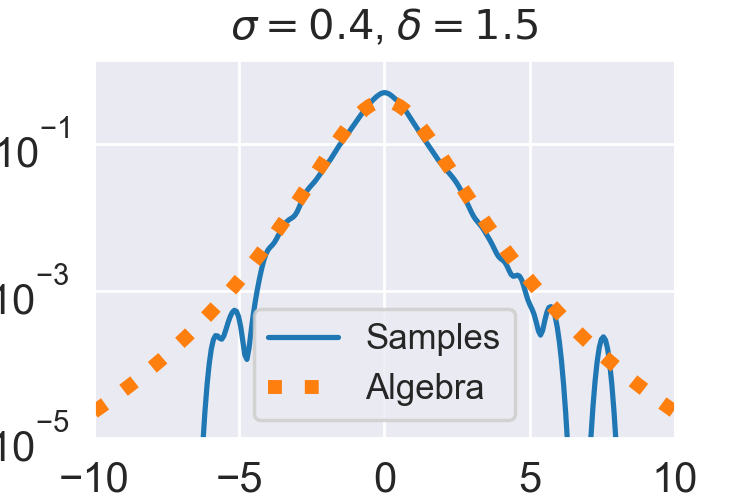
\includegraphics[width=0.32\textwidth]{figures/Kesten_0.40_1.5.png}
  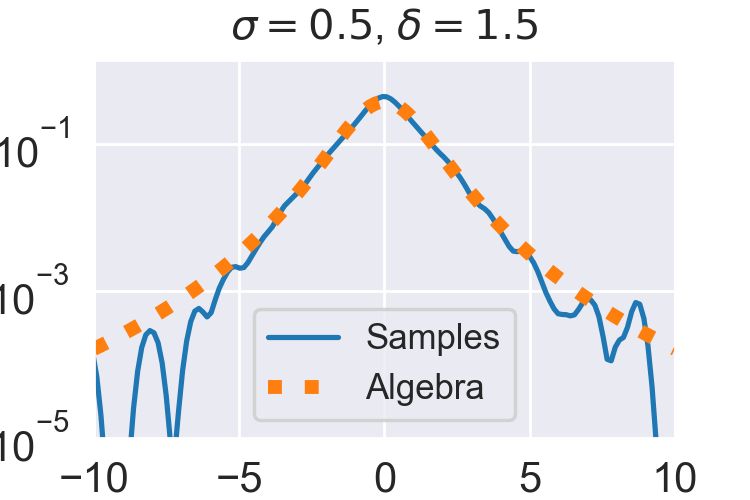
\includegraphics[width=0.32\textwidth]{figures/Kesten_0.50_1.5.png}
  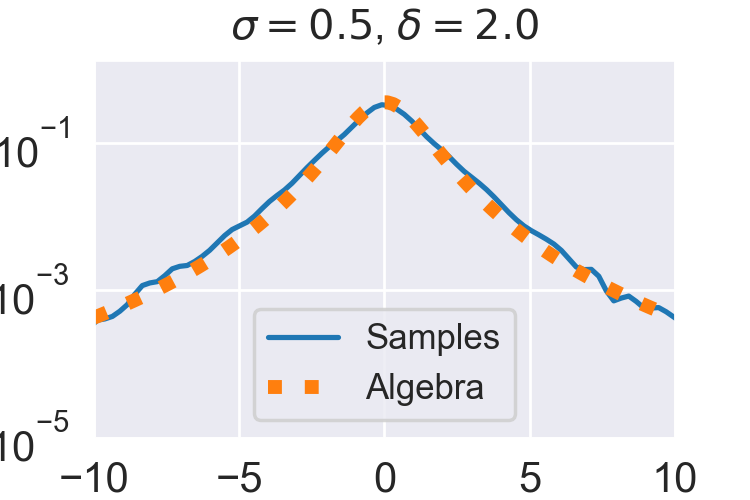
\includegraphics[width=0.32\textwidth]{figures/Kesten_0.50_2.png}
  \caption{\label{fig:SGD}Density of iterates of SGD vs. predicted tail behaviour}
\end{figure}

For inputs $X$ and labels $Y$ from a dataset $\mathcal{D}$, the least squares estimator for linear regression satisfies $\beta = \min_\beta \tfrac12 \mathbb{E}_{X,Y\sim\mathcal{D}}(Y - X\beta)^2$. To solve for this estimator, one can apply stochastic gradient descent (SGD) sampling over independent $X_k,Y_k\sim \mathcal{D}$ to obtain the sequence of iterations
\[
  \beta_{k+1} = (I - \delta X_k X_k^\top) \beta_k + \delta Y_k X_k
\]
for a step size $\delta > 0$. For large $\delta$, the iterates $\beta_k$ typically exhibit heavy-tailed fluctuations; in this regard, this sequence of iterates has been used as a simple model for more general stochastic optimization dynamics \citep{gurbuzbalaban2021heavy,hodgkinson2021multiplicative}. In particular, generalization performance has been tied to the heaviness of the tails in the iterates \cite{simsekli2019tail}. Here we use our algebra to predict the tail behaviour in a simple one-dimensional setting where $X_k \sim \mathcal{N}(0,\sigma^2)$ and $Y_k \sim \mathcal{N}(0,1)$. From classical theory \citep{buraczewski2016stochastic}, it is known that $X_k$ converges in distribution to a power law with tail exponent $\alpha > 0$ satisfying $\mathbb{E}|1 - \delta X_k^2|^\alpha = 1$. In \cref{fig:SGD}, we plot the density of the representative obtained using our algebra after $10^4$ iterations against a kernel density estimate of the first $10^6$ iterates when $\sigma \in \{0.4,0.5\}$ and $\delta \in \{1.5,2.0\}$. In all cases, the density obtained from the algebra provides a surprisingly close fit.



\subsection{Normal target}

Consider the toy example of a Normal target. This case is trivial for
Gaussian based methods and is oftentimes the initialization.
This lack of approximation gap in ADVI is seen in \Cref{fig:normal},
where we also see that GGA achieves similar approximation quality.
This is unsurprising as the GGA approximation in \Cref{tab:dist_list}
is also a Normal distribution.

\begin{figure}
  \centering
  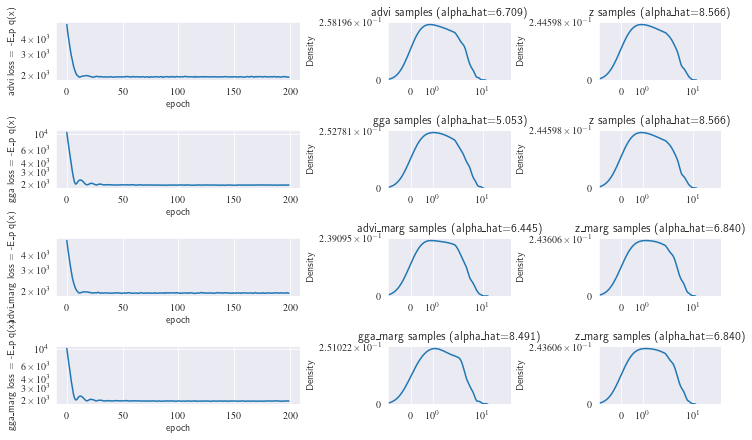
\includegraphics[width=1.0\textwidth]{figures/de_normal_sum.png}
  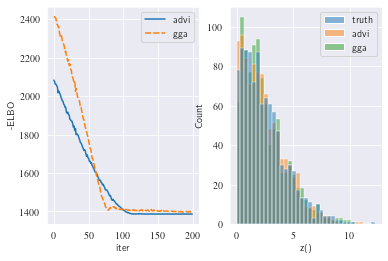
\includegraphics[width=.4\textwidth]{figures/vi_normal_sum.png}
  \caption{Density estimation and VI against a known normal target}
  \label{fig:normal}
\end{figure}


\subsection{Chi-square}

Now let $X_{ij} \sim N(0,1)$ and consider $tr X^\top X$.
Such quantities arise in the analysis of random projections.
It is important here to recognize that the power operation $X \mapsto X^2$ is not equivalent to the multiplication operation $X \mapsto X \otimes X$, as multiplication assumes independence.
\begin{figure}
  \centering
  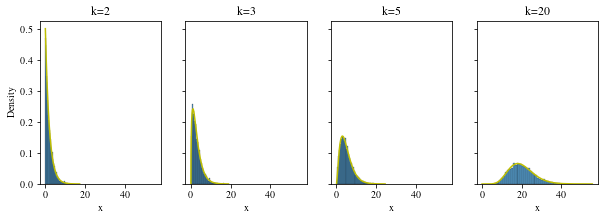
\includegraphics[width=\textwidth]{figures/jl-chi2.png}
  \caption{$5000$ samples of JL matrix trace (blue) vs GGA prediction (yellow)}
  \label{fig:jl_chi2}
\end{figure}



\section{Conclusion}\label{sec:hta:conclusion}

In this work, we have proposed a novel systematic approach for conducting tail inferential static analysis by implementing a three-parameter generalized Gamma algebra into a PPL compiler. Initial results are promising, showing that improved inference with simpler approximation families is possible when combined with tail metadata.
While already useful, the generalized Gamma algebra and its implementation currently has
some notable limitations:
\begin{itemize}[leftmargin=*]
  \item Since the algebra assumes independence, handling of dependencies between defined random variables must be conducted externally. This will inevitably require interoperability with a symbolic package to decompose complex expressions into operations on independent random variables.
  \item The GGA is formulated for univariate distributions only. Suitably defining multivariate tails is an open problem with interesting alternatives \citep{jaini2020tails,ftvi} all of which
        could extend GGA to higher dimensions.
  \item Conditioning is arguably the most important feature of a PPL and what distinguishes it from a glorified simulator. Exact marginalization in general is NP-hard \citep{koller2009probabilistic}, so treatment of conditional distributions using symbolic manipulations is a significant open problem, with some basic developments \cite{shan2017exact,cho2019disintegration}. Since only the tails are required in our setup, it may be possible to construct a dual algebra for operations under conditioning; this is left for future work.
  \item Compile-time static analysis only applicable to fixed model structure. While out of scope for our current work, open-universe models \citep{milch2010extending}
        and PPLs to support them \citep{bingham2019pyro} are an important research direction.
  \item The most significant omission to the algebra itself is classification of log-normal tails; while addition may be treated using \cite{gulisashvili2016tail} for example, multiplicative convolution with log-normal tails remains elusive.
  \item At present, reciprocals are approximated by assuming behaviour near zero. Reciprocals may be better treated by covering near-zero asymptotics separately.
\end{itemize}

The GGA provides a necessary first step into the static analysis of tails in
a probabilistic program.
As the above limitations are improved in future work and GGA becomes more broadly applicable,
we are excited to see how improved tail modelling will improve downstream PPL applications
as well as
other researchers will utilize GGA metadata to develop
novel PPL applications.

% \begin{ack}
% 	Use unnumbered first level headings for the acknowledgments. All acknowledgments
% 	go at the end of the paper before the list of references. Moreover, you are required to declare
% 	funding (financial activities supporting the submitted work) and competing interests (related financial activities outside the submitted work).
% 	More information about this disclosure can be found at: \url{https://neurips.cc/Conferences/2021/PaperInformation/FundingDisclosure}.

% 	Do {\bf not} include this section in the anonymized submission, only in the final paper. You can use the \texttt{ack} environment provided in the style file to autmoatically hide this section in the anonymized submission.
% \end{ack}

% \subsection{Limitations}

% \todo{Liam: Log-Normal insensitivity, edge case (see example)}

% The GGA is formulated for univariate distributions only. 

% {
% \small
% \bibliographystyle{unsrtnat}
% \bibliography{refs}
% }
%%%%%%%%%%%%%%%%%%%%%%%%%%%%%%%%%%%%%%%%%%%%%%%%%%%%%%%%%%%%
% \section*{Checklist}


% %%% BEGIN INSTRUCTIONS %%%
% The checklist follows the references.  Please
% read the checklist guidelines carefully for information on how to answer these
% questions.  For each question, change the default \answerTODO{} to \answerYes{},
% \answerNo{}, or \answerNA{}.  You are strongly encouraged to include a {\bf
% justification to your answer}, either by referencing the appropriate section of
% your paper or providing a brief inline description.  For example:
% \begin{itemize}
%   \item Did you include the license to the code and datasets? \answerYes{See Section~\ref{gen_inst}.}
%   \item Did you include the license to the code and datasets? \answerNo{The code and the data are proprietary.}
%   \item Did you include the license to the code and datasets? \answerNA{}
% \end{itemize}
% Please do not modify the questions and only use the provided macros for your
% answers.  Note that the Checklist section does not count towards the page
% limit.  In your paper, please delete this instructions block and only keep the
% Checklist section heading above along with the questions/answers below.
% %%% END INSTRUCTIONS %%%


% \begin{enumerate}

% \item For all authors...
% \begin{enumerate}
%   \item Do the main claims made in the abstract and introduction accurately reflect the paper's contributions and scope?
%     \answerYes{}
%   \item Did you describe the limitations of your work?
%     \answerYes{See \cref{sec:hta:conclusion}}
%   \item Did you discuss any potential negative societal impacts of your work?
%     \answerYes{See \cref{sec:hta:conclusion}}
%   \item Have you read the ethics review guidelines and ensured that your paper conforms to them?
%     \answerYes{}
% \end{enumerate}

% \item If you are including theoretical results...
% \begin{enumerate}
%   \item Did you state the full set of assumptions of all theoretical results?
%     \answerYes{Stated at start of \cref{sec:gga}}
% 	\item Did you include complete proofs of all theoretical results?
%     \answerYes{Most are deferred to supplementary materials}
% \end{enumerate}

% \item If you ran experiments...
% \begin{enumerate}
%   \item Did you include the code, data, and instructions needed to reproduce the main experimental results (either in the supplemental material or as a URL)?
%     \answerYes{See supplemental, a URL for code will be provided witn camera ready}
%   \item Did you specify all the training details (e.g., data splits, hyperparameters, how they were chosen)?
%     \answerYes{}
% 	\item Did you report error bars (e.g., with respect to the random seed after running experiments multiple times)?
%     \answerYes{Standard errors reported in parenthesis on \cref{tab:de} and \cref{tab:vi}}
% 	\item Did you include the total amount of compute and the type of resources used (e.g., type of GPUs, internal cluster, or cloud provider)?
%     \answerYes{See \cref{sec:hta:experiments}}
% \end{enumerate}

% \item If you are using existing assets (e.g., code, data, models) or curating/releasing new assets...
% \begin{enumerate}
%   \item If your work uses existing assets, did you cite the creators?
%     \answerYes{See citations of \citep{tehrani2020bean}}
%   \item Did you mention the license of the assets?
%     \answerYes{Licence included in code}
%   \item Did you include any new assets either in the supplemental material or as a URL?
%     \answerYes{See supplemental material}
%   \item Did you discuss whether and how consent was obtained from people whose data you're using/curating?
%     \answerNA{}
%   \item Did you discuss whether the data you are using/curating contains personally identifiable information or offensive content?
%     \answerNA{}
% \end{enumerate}

% \item If you used crowdsourcing or conducted research with human subjects...
% \begin{enumerate}
%   \item Did you include the full text of instructions given to participants and screenshots, if applicable?
%     \answerNA{}
%   \item Did you describe any potential participant risks, with links to Institutional Review Board (IRB) approvals, if applicable?
%     \answerNA{}
%   \item Did you include the estimated hourly wage paid to participants and the total amount spent on participant compensation?
%     \answerNA{}
% \end{enumerate}

% \end{enumerate}

%%%%%%%%%%%%%%%%%%%%%%%%%%%%%%%%%%%%%%%%%%%%%%%%%%%%%%%%%%%%
% \ifdefined\remappendix
% \newpage

% \appendix




% \fi
\end{document}
